\documentclass[twoside]{book}

% Packages required by doxygen
\usepackage{fixltx2e}
\usepackage{calc}
\usepackage{doxygen}
\usepackage[export]{adjustbox} % also loads graphicx
\usepackage{graphicx}
\usepackage[utf8]{inputenc}
\usepackage{makeidx}
\usepackage{multicol}
\usepackage{multirow}
\PassOptionsToPackage{warn}{textcomp}
\usepackage{textcomp}
\usepackage[nointegrals]{wasysym}
\usepackage[table]{xcolor}

% NLS support packages
\usepackage[french]{babel}

% Font selection
\usepackage[T1]{fontenc}
\usepackage[scaled=.90]{helvet}
\usepackage{courier}
\usepackage{amssymb}
\usepackage{sectsty}
\renewcommand{\familydefault}{\sfdefault}
\allsectionsfont{%
  \fontseries{bc}\selectfont%
  \color{darkgray}%
}
\renewcommand{\DoxyLabelFont}{%
  \fontseries{bc}\selectfont%
  \color{darkgray}%
}
\newcommand{\+}{\discretionary{\mbox{\scriptsize$\hookleftarrow$}}{}{}}

% Page & text layout
\usepackage{geometry}
\geometry{%
  a4paper,%
  top=2.5cm,%
  bottom=2.5cm,%
  left=2.5cm,%
  right=2.5cm%
}
\tolerance=750
\hfuzz=15pt
\hbadness=750
\setlength{\emergencystretch}{15pt}
\setlength{\parindent}{0cm}
\setlength{\parskip}{3ex plus 2ex minus 2ex}
\makeatletter
\renewcommand{\paragraph}{%
  \@startsection{paragraph}{4}{0ex}{-1.0ex}{1.0ex}{%
    \normalfont\normalsize\bfseries\SS@parafont%
  }%
}
\renewcommand{\subparagraph}{%
  \@startsection{subparagraph}{5}{0ex}{-1.0ex}{1.0ex}{%
    \normalfont\normalsize\bfseries\SS@subparafont%
  }%
}
\makeatother

% Headers & footers
\usepackage{fancyhdr}
\pagestyle{fancyplain}
\fancyhead[LE]{\fancyplain{}{\bfseries\thepage}}
\fancyhead[CE]{\fancyplain{}{}}
\fancyhead[RE]{\fancyplain{}{\bfseries\leftmark}}
\fancyhead[LO]{\fancyplain{}{\bfseries\rightmark}}
\fancyhead[CO]{\fancyplain{}{}}
\fancyhead[RO]{\fancyplain{}{\bfseries\thepage}}
\fancyfoot[LE]{\fancyplain{}{}}
\fancyfoot[CE]{\fancyplain{}{}}
\fancyfoot[RE]{\fancyplain{}{\bfseries\scriptsize Généré par Doxygen }}
\fancyfoot[LO]{\fancyplain{}{\bfseries\scriptsize Généré par Doxygen }}
\fancyfoot[CO]{\fancyplain{}{}}
\fancyfoot[RO]{\fancyplain{}{}}
\renewcommand{\footrulewidth}{0.4pt}
\renewcommand{\chaptermark}[1]{%
  \markboth{#1}{}%
}
\renewcommand{\sectionmark}[1]{%
  \markright{\thesection\ #1}%
}

% Indices & bibliography
\usepackage{natbib}
\usepackage[titles]{tocloft}
\setcounter{tocdepth}{3}
\setcounter{secnumdepth}{5}
\makeindex

% Hyperlinks (required, but should be loaded last)
\usepackage{ifpdf}
\ifpdf
  \usepackage[pdftex,pagebackref=true]{hyperref}
\else
  \usepackage[ps2pdf,pagebackref=true]{hyperref}
\fi
\hypersetup{%
  colorlinks=true,%
  linkcolor=blue,%
  citecolor=blue,%
  unicode%
}

% Custom commands
\newcommand{\clearemptydoublepage}{%
  \newpage{\pagestyle{empty}\cleardoublepage}%
}

\usepackage{caption}
\captionsetup{labelsep=space,justification=centering,font={bf},singlelinecheck=off,skip=4pt,position=top}

%===== C O N T E N T S =====

\begin{document}

% Titlepage & ToC
\hypersetup{pageanchor=false,
             bookmarksnumbered=true,
             pdfencoding=unicode
            }
\pagenumbering{alph}
\begin{titlepage}
\vspace*{7cm}
\begin{center}%
{\Large M\+B\+E\+S-\/decode \\[1ex]\large C\+U\+R\+R\+E\+N\+T\+\_\+\+V\+E\+R\+S\+I\+O\+N\+\_\+\+O\+F\+\_\+\+M\+B\+E\+S\+\_\+\+D\+E\+C\+O\+DE }\\
\vspace*{1cm}
{\large Généré par Doxygen 1.8.13}\\
\end{center}
\end{titlepage}
\clearemptydoublepage
\pagenumbering{roman}
\tableofcontents
\clearemptydoublepage
\pagenumbering{arabic}
\hypersetup{pageanchor=true}

%--- Begin generated contents ---
\chapter{Index hiérarchique}
\section{Hiérarchie des classes}
Cette liste d\textquotesingle{}héritage est classée approximativement par ordre alphabétique \+:\begin{DoxyCompactList}
\item \contentsline{section}{Kongsberg\+Attitude\+Entry}{\pageref{structKongsbergAttitudeEntry}}{}
\item \contentsline{section}{Kongsberg\+Header}{\pageref{structKongsbergHeader}}{}
\item \contentsline{section}{Kongsberg\+Position\+Datagram}{\pageref{structKongsbergPositionDatagram}}{}
\item \contentsline{section}{Mbes\+Parser}{\pageref{classMbesParser}}{}
\begin{DoxyCompactList}
\item \contentsline{section}{Kongsberg\+Parser}{\pageref{classKongsbergParser}}{}
\item \contentsline{section}{Xtf\+Parser}{\pageref{classXtfParser}}{}
\end{DoxyCompactList}
\item \contentsline{section}{Nmea\+Utils}{\pageref{classNmeaUtils}}{}
\item \contentsline{section}{S\+N\+P0}{\pageref{structSNP0}}{}
\item \contentsline{section}{S\+N\+P1}{\pageref{structSNP1}}{}
\item \contentsline{section}{Xtf\+Attitude\+Data}{\pageref{structXtfAttitudeData}}{}
\item \contentsline{section}{Xtf\+Beam\+X\+Y\+ZA}{\pageref{structXtfBeamXYZA}}{}
\item \contentsline{section}{Xtf\+Chan\+Info}{\pageref{structXtfChanInfo}}{}
\item \contentsline{section}{Xtf\+File\+Header}{\pageref{structXtfFileHeader}}{}
\item \contentsline{section}{Xtf\+Header\+Gyro}{\pageref{structXtfHeaderGyro}}{}
\item \contentsline{section}{Xtf\+Header\+Navigation\+\_\+type42}{\pageref{structXtfHeaderNavigation__type42}}{}
\item \contentsline{section}{Xtf\+Header\+Navigation\+\_\+type84}{\pageref{structXtfHeaderNavigation__type84}}{}
\item \contentsline{section}{Xtf\+High\+Speed\+Sensor}{\pageref{structXtfHighSpeedSensor}}{}
\item \contentsline{section}{Xtf\+Notes\+Header}{\pageref{structXtfNotesHeader}}{}
\item \contentsline{section}{Xtf\+Packet\+Header}{\pageref{structXtfPacketHeader}}{}
\item \contentsline{section}{Xtf\+Ping\+Chan\+Header}{\pageref{structXtfPingChanHeader}}{}
\item \contentsline{section}{Xtf\+Ping\+Header}{\pageref{structXtfPingHeader}}{}
\item \contentsline{section}{Xtf\+Pos\+Raw\+Navigation}{\pageref{structXtfPosRawNavigation}}{}
\item \contentsline{section}{Xtf\+Qps\+Mb\+Entry}{\pageref{structXtfQpsMbEntry}}{}
\item \contentsline{section}{Xtf\+Qps\+Multi\+Tx\+Entry}{\pageref{structXtfQpsMultiTxEntry}}{}
\item \contentsline{section}{Xtf\+Qps\+Single\+Beam}{\pageref{structXtfQpsSingleBeam}}{}
\item \contentsline{section}{Xtf\+Raw\+Custom\+Header}{\pageref{structXtfRawCustomHeader}}{}
\item \contentsline{section}{Xtf\+Raw\+Serial\+Header}{\pageref{structXtfRawSerialHeader}}{}
\end{DoxyCompactList}

\chapter{Index des classes}
\section{Liste des classes}
Liste des classes, structures, unions et interfaces avec une brève description \+:\begin{DoxyCompactList}
\item\contentsline{section}{\hyperlink{structKongsbergAttitudeEntry}{Kongsberg\+Attitude\+Entry} }{\pageref{structKongsbergAttitudeEntry}}{}
\item\contentsline{section}{\hyperlink{structKongsbergHeader}{Kongsberg\+Header} }{\pageref{structKongsbergHeader}}{}
\item\contentsline{section}{\hyperlink{classKongsbergParser}{Kongsberg\+Parser} }{\pageref{classKongsbergParser}}{}
\item\contentsline{section}{\hyperlink{structKongsbergPositionDatagram}{Kongsberg\+Position\+Datagram} }{\pageref{structKongsbergPositionDatagram}}{}
\item\contentsline{section}{\hyperlink{classMbesParser}{Mbes\+Parser} }{\pageref{classMbesParser}}{}
\item\contentsline{section}{\hyperlink{classNmeaUtils}{Nmea\+Utils} }{\pageref{classNmeaUtils}}{}
\item\contentsline{section}{\hyperlink{structSNP0}{S\+N\+P0} }{\pageref{structSNP0}}{}
\item\contentsline{section}{\hyperlink{structSNP1}{S\+N\+P1} }{\pageref{structSNP1}}{}
\item\contentsline{section}{\hyperlink{structXtfAttitudeData}{Xtf\+Attitude\+Data} }{\pageref{structXtfAttitudeData}}{}
\item\contentsline{section}{\hyperlink{structXtfBeamXYZA}{Xtf\+Beam\+X\+Y\+ZA} }{\pageref{structXtfBeamXYZA}}{}
\item\contentsline{section}{\hyperlink{structXtfChanInfo}{Xtf\+Chan\+Info} \\*Description des datagrammes pour le format X\+TF Référence\+: Triton Imaging, Inc }{\pageref{structXtfChanInfo}}{}
\item\contentsline{section}{\hyperlink{structXtfFileHeader}{Xtf\+File\+Header} }{\pageref{structXtfFileHeader}}{}
\item\contentsline{section}{\hyperlink{structXtfHeaderGyro}{Xtf\+Header\+Gyro} }{\pageref{structXtfHeaderGyro}}{}
\item\contentsline{section}{\hyperlink{structXtfHeaderNavigation__type42}{Xtf\+Header\+Navigation\+\_\+type42} }{\pageref{structXtfHeaderNavigation__type42}}{}
\item\contentsline{section}{\hyperlink{structXtfHeaderNavigation__type84}{Xtf\+Header\+Navigation\+\_\+type84} }{\pageref{structXtfHeaderNavigation__type84}}{}
\item\contentsline{section}{\hyperlink{structXtfHighSpeedSensor}{Xtf\+High\+Speed\+Sensor} }{\pageref{structXtfHighSpeedSensor}}{}
\item\contentsline{section}{\hyperlink{structXtfNotesHeader}{Xtf\+Notes\+Header} }{\pageref{structXtfNotesHeader}}{}
\item\contentsline{section}{\hyperlink{structXtfPacketHeader}{Xtf\+Packet\+Header} }{\pageref{structXtfPacketHeader}}{}
\item\contentsline{section}{\hyperlink{classXtfParser}{Xtf\+Parser} }{\pageref{classXtfParser}}{}
\item\contentsline{section}{\hyperlink{structXtfPingChanHeader}{Xtf\+Ping\+Chan\+Header} }{\pageref{structXtfPingChanHeader}}{}
\item\contentsline{section}{\hyperlink{structXtfPingHeader}{Xtf\+Ping\+Header} }{\pageref{structXtfPingHeader}}{}
\item\contentsline{section}{\hyperlink{structXtfPosRawNavigation}{Xtf\+Pos\+Raw\+Navigation} }{\pageref{structXtfPosRawNavigation}}{}
\item\contentsline{section}{\hyperlink{structXtfQpsMbEntry}{Xtf\+Qps\+Mb\+Entry} }{\pageref{structXtfQpsMbEntry}}{}
\item\contentsline{section}{\hyperlink{structXtfQpsMultiTxEntry}{Xtf\+Qps\+Multi\+Tx\+Entry} }{\pageref{structXtfQpsMultiTxEntry}}{}
\item\contentsline{section}{\hyperlink{structXtfQpsSingleBeam}{Xtf\+Qps\+Single\+Beam} }{\pageref{structXtfQpsSingleBeam}}{}
\item\contentsline{section}{\hyperlink{structXtfRawCustomHeader}{Xtf\+Raw\+Custom\+Header} }{\pageref{structXtfRawCustomHeader}}{}
\item\contentsline{section}{\hyperlink{structXtfRawSerialHeader}{Xtf\+Raw\+Serial\+Header} }{\pageref{structXtfRawSerialHeader}}{}
\end{DoxyCompactList}

\chapter{Index des fichiers}
\section{Liste des fichiers}
Liste de tous les fichiers avec une brève description \+:\begin{DoxyCompactList}
\item\contentsline{section}{src/datagrams/\hyperlink{MbesParser_8hpp}{Mbes\+Parser.\+hpp} }{\pageref{MbesParser_8hpp}}{}
\item\contentsline{section}{src/datagrams/kongsberg/\hyperlink{KongsbergParser_8hpp}{Kongsberg\+Parser.\+hpp} }{\pageref{KongsbergParser_8hpp}}{}
\item\contentsline{section}{src/datagrams/kongsberg/\hyperlink{KongsbergTypes_8hpp}{Kongsberg\+Types.\+hpp} }{\pageref{KongsbergTypes_8hpp}}{}
\item\contentsline{section}{src/datagrams/xtf/\hyperlink{XtfParser_8hpp}{Xtf\+Parser.\+hpp} }{\pageref{XtfParser_8hpp}}{}
\item\contentsline{section}{src/datagrams/xtf/\hyperlink{XtfTypes_8hpp}{Xtf\+Types.\+hpp} }{\pageref{XtfTypes_8hpp}}{}
\item\contentsline{section}{src/examples/\hyperlink{datagram-dump_8cpp}{datagram-\/dump.\+cpp} }{\pageref{datagram-dump_8cpp}}{}
\item\contentsline{section}{src/utils/\hyperlink{NmeaUtils_8hpp}{Nmea\+Utils.\+hpp} }{\pageref{NmeaUtils_8hpp}}{}
\item\contentsline{section}{src/utils/\hyperlink{StringUtils_8hpp}{String\+Utils.\+hpp} }{\pageref{StringUtils_8hpp}}{}
\item\contentsline{section}{src/utils/\hyperlink{TimeUtils_8hpp}{Time\+Utils.\+hpp} }{\pageref{TimeUtils_8hpp}}{}
\end{DoxyCompactList}

\chapter{Documentation des classes}
\hypertarget{structKongsbergAttitudeEntry}{}\section{Référence de la structure Kongsberg\+Attitude\+Entry}
\label{structKongsbergAttitudeEntry}\index{Kongsberg\+Attitude\+Entry@{Kongsberg\+Attitude\+Entry}}


{\ttfamily \#include $<$Kongsberg\+Parser.\+hpp$>$}

\subsection*{Attributs publics}
\begin{DoxyCompactItemize}
\item 
uint16\+\_\+t \hyperlink{structKongsbergAttitudeEntry_a9b6a73b3b1fa67ee696e2ec73c0fe837}{Num\+Entries}
\item 
uint16\+\_\+t \hyperlink{structKongsbergAttitudeEntry_a300a0518f2405865a960816e561680b1}{delta\+Time}
\item 
int16\+\_\+t \hyperlink{structKongsbergAttitudeEntry_a130bbc4115e74b4932ca5a9787e944e4}{roll}
\item 
int16\+\_\+t \hyperlink{structKongsbergAttitudeEntry_ab4995036069d41a73c8f0dc11a8766ee}{pitch}
\item 
int16\+\_\+t \hyperlink{structKongsbergAttitudeEntry_a95140a0fd7d9982f0fb6c47573d7a594}{heave}
\item 
int16\+\_\+t \hyperlink{structKongsbergAttitudeEntry_a7dc42f0fdc8852f1d39270b761925535}{heading}
\end{DoxyCompactItemize}


\subsection{Documentation des données membres}
\mbox{\Hypertarget{structKongsbergAttitudeEntry_a300a0518f2405865a960816e561680b1}\label{structKongsbergAttitudeEntry_a300a0518f2405865a960816e561680b1}} 
\index{Kongsberg\+Attitude\+Entry@{Kongsberg\+Attitude\+Entry}!delta\+Time@{delta\+Time}}
\index{delta\+Time@{delta\+Time}!Kongsberg\+Attitude\+Entry@{Kongsberg\+Attitude\+Entry}}
\subsubsection{\texorpdfstring{delta\+Time}{deltaTime}}
{\footnotesize\ttfamily uint16\+\_\+t Kongsberg\+Attitude\+Entry\+::delta\+Time}

\mbox{\Hypertarget{structKongsbergAttitudeEntry_a7dc42f0fdc8852f1d39270b761925535}\label{structKongsbergAttitudeEntry_a7dc42f0fdc8852f1d39270b761925535}} 
\index{Kongsberg\+Attitude\+Entry@{Kongsberg\+Attitude\+Entry}!heading@{heading}}
\index{heading@{heading}!Kongsberg\+Attitude\+Entry@{Kongsberg\+Attitude\+Entry}}
\subsubsection{\texorpdfstring{heading}{heading}}
{\footnotesize\ttfamily int16\+\_\+t Kongsberg\+Attitude\+Entry\+::heading}

\mbox{\Hypertarget{structKongsbergAttitudeEntry_a95140a0fd7d9982f0fb6c47573d7a594}\label{structKongsbergAttitudeEntry_a95140a0fd7d9982f0fb6c47573d7a594}} 
\index{Kongsberg\+Attitude\+Entry@{Kongsberg\+Attitude\+Entry}!heave@{heave}}
\index{heave@{heave}!Kongsberg\+Attitude\+Entry@{Kongsberg\+Attitude\+Entry}}
\subsubsection{\texorpdfstring{heave}{heave}}
{\footnotesize\ttfamily int16\+\_\+t Kongsberg\+Attitude\+Entry\+::heave}

\mbox{\Hypertarget{structKongsbergAttitudeEntry_a9b6a73b3b1fa67ee696e2ec73c0fe837}\label{structKongsbergAttitudeEntry_a9b6a73b3b1fa67ee696e2ec73c0fe837}} 
\index{Kongsberg\+Attitude\+Entry@{Kongsberg\+Attitude\+Entry}!Num\+Entries@{Num\+Entries}}
\index{Num\+Entries@{Num\+Entries}!Kongsberg\+Attitude\+Entry@{Kongsberg\+Attitude\+Entry}}
\subsubsection{\texorpdfstring{Num\+Entries}{NumEntries}}
{\footnotesize\ttfamily uint16\+\_\+t Kongsberg\+Attitude\+Entry\+::\+Num\+Entries}

\mbox{\Hypertarget{structKongsbergAttitudeEntry_ab4995036069d41a73c8f0dc11a8766ee}\label{structKongsbergAttitudeEntry_ab4995036069d41a73c8f0dc11a8766ee}} 
\index{Kongsberg\+Attitude\+Entry@{Kongsberg\+Attitude\+Entry}!pitch@{pitch}}
\index{pitch@{pitch}!Kongsberg\+Attitude\+Entry@{Kongsberg\+Attitude\+Entry}}
\subsubsection{\texorpdfstring{pitch}{pitch}}
{\footnotesize\ttfamily int16\+\_\+t Kongsberg\+Attitude\+Entry\+::pitch}

\mbox{\Hypertarget{structKongsbergAttitudeEntry_a130bbc4115e74b4932ca5a9787e944e4}\label{structKongsbergAttitudeEntry_a130bbc4115e74b4932ca5a9787e944e4}} 
\index{Kongsberg\+Attitude\+Entry@{Kongsberg\+Attitude\+Entry}!roll@{roll}}
\index{roll@{roll}!Kongsberg\+Attitude\+Entry@{Kongsberg\+Attitude\+Entry}}
\subsubsection{\texorpdfstring{roll}{roll}}
{\footnotesize\ttfamily int16\+\_\+t Kongsberg\+Attitude\+Entry\+::roll}



La documentation de cette structure a été générée à partir du fichier suivant \+:\begin{DoxyCompactItemize}
\item 
src/datagrams/kongsberg/\hyperlink{KongsbergParser_8hpp}{Kongsberg\+Parser.\+hpp}\end{DoxyCompactItemize}

\hypertarget{structKongsbergHeader}{}\section{Référence de la structure Kongsberg\+Header}
\label{structKongsbergHeader}\index{Kongsberg\+Header@{Kongsberg\+Header}}


{\ttfamily \#include $<$Kongsberg\+Parser.\+hpp$>$}

\subsection*{Attributs publics}
\begin{DoxyCompactItemize}
\item 
uint32\+\_\+t \hyperlink{structKongsbergHeader_a15e4621707e24d4904395d3a1e26a9fe}{size}
\item 
unsigned char \hyperlink{structKongsbergHeader_a919858cc5e98d8f3182091ea2fba2531}{stx}
\item 
unsigned char \hyperlink{structKongsbergHeader_a53429e4241d2b6f9163ece6ff6eae4d3}{type}
\item 
uint16\+\_\+t \hyperlink{structKongsbergHeader_a6ec045b8677927f8c7bfa7b71481e424}{model\+Number}
\item 
uint32\+\_\+t \hyperlink{structKongsbergHeader_a43b7d1f638a2264ee629faf5ff920326}{date}
\item 
uint32\+\_\+t \hyperlink{structKongsbergHeader_aa9701e6d9deaf91ce47631221b50ec6c}{time}
\item 
uint16\+\_\+t \hyperlink{structKongsbergHeader_a15fc213f2eecb5a01c9d042ea57fcdd7}{counter}
\item 
uint16\+\_\+t \hyperlink{structKongsbergHeader_afd878130f79841cefe289aeceb79f970}{serial\+Number}
\end{DoxyCompactItemize}


\subsection{Documentation des données membres}
\mbox{\Hypertarget{structKongsbergHeader_a15fc213f2eecb5a01c9d042ea57fcdd7}\label{structKongsbergHeader_a15fc213f2eecb5a01c9d042ea57fcdd7}} 
\index{Kongsberg\+Header@{Kongsberg\+Header}!counter@{counter}}
\index{counter@{counter}!Kongsberg\+Header@{Kongsberg\+Header}}
\subsubsection{\texorpdfstring{counter}{counter}}
{\footnotesize\ttfamily uint16\+\_\+t Kongsberg\+Header\+::counter}

\mbox{\Hypertarget{structKongsbergHeader_a43b7d1f638a2264ee629faf5ff920326}\label{structKongsbergHeader_a43b7d1f638a2264ee629faf5ff920326}} 
\index{Kongsberg\+Header@{Kongsberg\+Header}!date@{date}}
\index{date@{date}!Kongsberg\+Header@{Kongsberg\+Header}}
\subsubsection{\texorpdfstring{date}{date}}
{\footnotesize\ttfamily uint32\+\_\+t Kongsberg\+Header\+::date}

\mbox{\Hypertarget{structKongsbergHeader_a6ec045b8677927f8c7bfa7b71481e424}\label{structKongsbergHeader_a6ec045b8677927f8c7bfa7b71481e424}} 
\index{Kongsberg\+Header@{Kongsberg\+Header}!model\+Number@{model\+Number}}
\index{model\+Number@{model\+Number}!Kongsberg\+Header@{Kongsberg\+Header}}
\subsubsection{\texorpdfstring{model\+Number}{modelNumber}}
{\footnotesize\ttfamily uint16\+\_\+t Kongsberg\+Header\+::model\+Number}

\mbox{\Hypertarget{structKongsbergHeader_afd878130f79841cefe289aeceb79f970}\label{structKongsbergHeader_afd878130f79841cefe289aeceb79f970}} 
\index{Kongsberg\+Header@{Kongsberg\+Header}!serial\+Number@{serial\+Number}}
\index{serial\+Number@{serial\+Number}!Kongsberg\+Header@{Kongsberg\+Header}}
\subsubsection{\texorpdfstring{serial\+Number}{serialNumber}}
{\footnotesize\ttfamily uint16\+\_\+t Kongsberg\+Header\+::serial\+Number}

\mbox{\Hypertarget{structKongsbergHeader_a15e4621707e24d4904395d3a1e26a9fe}\label{structKongsbergHeader_a15e4621707e24d4904395d3a1e26a9fe}} 
\index{Kongsberg\+Header@{Kongsberg\+Header}!size@{size}}
\index{size@{size}!Kongsberg\+Header@{Kongsberg\+Header}}
\subsubsection{\texorpdfstring{size}{size}}
{\footnotesize\ttfamily uint32\+\_\+t Kongsberg\+Header\+::size}

\mbox{\Hypertarget{structKongsbergHeader_a919858cc5e98d8f3182091ea2fba2531}\label{structKongsbergHeader_a919858cc5e98d8f3182091ea2fba2531}} 
\index{Kongsberg\+Header@{Kongsberg\+Header}!stx@{stx}}
\index{stx@{stx}!Kongsberg\+Header@{Kongsberg\+Header}}
\subsubsection{\texorpdfstring{stx}{stx}}
{\footnotesize\ttfamily unsigned char Kongsberg\+Header\+::stx}

\mbox{\Hypertarget{structKongsbergHeader_aa9701e6d9deaf91ce47631221b50ec6c}\label{structKongsbergHeader_aa9701e6d9deaf91ce47631221b50ec6c}} 
\index{Kongsberg\+Header@{Kongsberg\+Header}!time@{time}}
\index{time@{time}!Kongsberg\+Header@{Kongsberg\+Header}}
\subsubsection{\texorpdfstring{time}{time}}
{\footnotesize\ttfamily uint32\+\_\+t Kongsberg\+Header\+::time}

\mbox{\Hypertarget{structKongsbergHeader_a53429e4241d2b6f9163ece6ff6eae4d3}\label{structKongsbergHeader_a53429e4241d2b6f9163ece6ff6eae4d3}} 
\index{Kongsberg\+Header@{Kongsberg\+Header}!type@{type}}
\index{type@{type}!Kongsberg\+Header@{Kongsberg\+Header}}
\subsubsection{\texorpdfstring{type}{type}}
{\footnotesize\ttfamily unsigned char Kongsberg\+Header\+::type}



La documentation de cette structure a été générée à partir du fichier suivant \+:\begin{DoxyCompactItemize}
\item 
src/datagrams/kongsberg/\hyperlink{KongsbergParser_8hpp}{Kongsberg\+Parser.\+hpp}\end{DoxyCompactItemize}

\hypertarget{classKongsbergParser}{}\section{Référence de la classe Kongsberg\+Parser}
\label{classKongsbergParser}\index{Kongsberg\+Parser@{Kongsberg\+Parser}}


{\ttfamily \#include $<$Kongsberg\+Parser.\+hpp$>$}



Graphe d\textquotesingle{}héritage de Kongsberg\+Parser\+:
\nopagebreak
\begin{figure}[H]
\begin{center}
\leavevmode
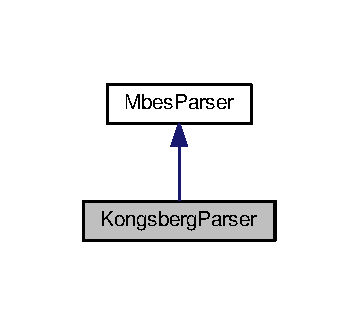
\includegraphics[width=172pt]{classKongsbergParser__inherit__graph}
\end{center}
\end{figure}


Graphe de collaboration de Kongsberg\+Parser\+:
\nopagebreak
\begin{figure}[H]
\begin{center}
\leavevmode
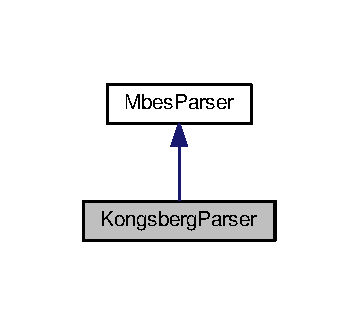
\includegraphics[width=172pt]{classKongsbergParser__coll__graph}
\end{center}
\end{figure}
\subsection*{Fonctions membres publiques}
\begin{DoxyCompactItemize}
\item 
\hyperlink{classKongsbergParser_a9a756a45d8d6ba1f83567685daf23f91}{Kongsberg\+Parser} ()
\item 
\hyperlink{classKongsbergParser_a7500ac454b264049e6f2078d914e86da}{$\sim$\+Kongsberg\+Parser} ()
\item 
void \hyperlink{classKongsbergParser_af7c31817a75fc4d153945f35f08b9d99}{parse} (std\+::string filename)
\item 
void \hyperlink{classKongsbergParser_aa241961b762eb4fed4702a337573d46d}{process\+Attitude} (uint64\+\_\+t micro\+Epoch, double heading, double pitch, double roll)
\item 
void \hyperlink{classKongsbergParser_a692580461f3e6d8f822cb84cf3ed6a3c}{process\+Position} (uint64\+\_\+t micro\+Epoch, double longitude, double latitude, double height)
\end{DoxyCompactItemize}
\subsection*{Fonctions membres privées}
\begin{DoxyCompactItemize}
\item 
void \hyperlink{classKongsbergParser_a4d2236cb102afd4eef21687f5032e7fa}{process\+Datagram} (\hyperlink{structKongsbergHeader}{Kongsberg\+Header} \&hdr, unsigned char $\ast$datagram)
\item 
void \hyperlink{classKongsbergParser_a4ece0df376ad28782f7a59d2557b42df}{process\+Depth} (\hyperlink{structKongsbergHeader}{Kongsberg\+Header} \&hdr, unsigned char $\ast$datagram)
\item 
void \hyperlink{classKongsbergParser_a9af87754001eb5c6fa6761146a78e29e}{process\+Water\+Height} (\hyperlink{structKongsbergHeader}{Kongsberg\+Header} \&hdr, unsigned char $\ast$datagram)
\item 
void \hyperlink{classKongsbergParser_a2404c01d8852893a2b93e68b2841ba66}{process\+Attitude\+Datagram} (\hyperlink{structKongsbergHeader}{Kongsberg\+Header} \&hdr, unsigned char $\ast$datagram)
\item 
void \hyperlink{classKongsbergParser_a2d81dc1b6ba8e7fd055add0009a87366}{process\+Position\+Datagram} (\hyperlink{structKongsbergHeader}{Kongsberg\+Header} \&hdr, unsigned char $\ast$datagram)
\item 
void \hyperlink{classKongsbergParser_a1edd36292b5098e2969fb3ecd0a88abb}{process\+Quality\+Factor} (\hyperlink{structKongsbergHeader}{Kongsberg\+Header} \&hdr, unsigned char $\ast$datagram)
\item 
void \hyperlink{classKongsbergParser_afa9fad0b7e76896ca18294c145353c87}{process\+Seabed\+Image\+Data} (\hyperlink{structKongsbergHeader}{Kongsberg\+Header} \&hdr, unsigned char $\ast$datagram)
\item 
long \hyperlink{classKongsbergParser_a916ac4169f44591ae5d768545f6081fc}{convert\+Time} (long datagram\+Date, long datagram\+Time)
\end{DoxyCompactItemize}


\subsection{Documentation des constructeurs et destructeur}
\mbox{\Hypertarget{classKongsbergParser_a9a756a45d8d6ba1f83567685daf23f91}\label{classKongsbergParser_a9a756a45d8d6ba1f83567685daf23f91}} 
\index{Kongsberg\+Parser@{Kongsberg\+Parser}!Kongsberg\+Parser@{Kongsberg\+Parser}}
\index{Kongsberg\+Parser@{Kongsberg\+Parser}!Kongsberg\+Parser@{Kongsberg\+Parser}}
\subsubsection{\texorpdfstring{Kongsberg\+Parser()}{KongsbergParser()}}
{\footnotesize\ttfamily Kongsberg\+Parser\+::\+Kongsberg\+Parser (\begin{DoxyParamCaption}{ }\end{DoxyParamCaption})}

\mbox{\Hypertarget{classKongsbergParser_a7500ac454b264049e6f2078d914e86da}\label{classKongsbergParser_a7500ac454b264049e6f2078d914e86da}} 
\index{Kongsberg\+Parser@{Kongsberg\+Parser}!````~Kongsberg\+Parser@{$\sim$\+Kongsberg\+Parser}}
\index{````~Kongsberg\+Parser@{$\sim$\+Kongsberg\+Parser}!Kongsberg\+Parser@{Kongsberg\+Parser}}
\subsubsection{\texorpdfstring{$\sim$\+Kongsberg\+Parser()}{~KongsbergParser()}}
{\footnotesize\ttfamily Kongsberg\+Parser\+::$\sim$\+Kongsberg\+Parser (\begin{DoxyParamCaption}{ }\end{DoxyParamCaption})}



\subsection{Documentation des fonctions membres}
\mbox{\Hypertarget{classKongsbergParser_a916ac4169f44591ae5d768545f6081fc}\label{classKongsbergParser_a916ac4169f44591ae5d768545f6081fc}} 
\index{Kongsberg\+Parser@{Kongsberg\+Parser}!convert\+Time@{convert\+Time}}
\index{convert\+Time@{convert\+Time}!Kongsberg\+Parser@{Kongsberg\+Parser}}
\subsubsection{\texorpdfstring{convert\+Time()}{convertTime()}}
{\footnotesize\ttfamily long Kongsberg\+Parser\+::convert\+Time (\begin{DoxyParamCaption}\item[{long}]{datagram\+Date,  }\item[{long}]{datagram\+Time }\end{DoxyParamCaption})\hspace{0.3cm}{\ttfamily [private]}}

\mbox{\Hypertarget{classKongsbergParser_af7c31817a75fc4d153945f35f08b9d99}\label{classKongsbergParser_af7c31817a75fc4d153945f35f08b9d99}} 
\index{Kongsberg\+Parser@{Kongsberg\+Parser}!parse@{parse}}
\index{parse@{parse}!Kongsberg\+Parser@{Kongsberg\+Parser}}
\subsubsection{\texorpdfstring{parse()}{parse()}}
{\footnotesize\ttfamily void Kongsberg\+Parser\+::parse (\begin{DoxyParamCaption}\item[{std\+::string}]{filename }\end{DoxyParamCaption})\hspace{0.3cm}{\ttfamily [virtual]}}



Réimplémentée à partir de \hyperlink{classMbesParser_a10e172520c1ca2b87dab51aef9e57c2a}{Mbes\+Parser}.

\mbox{\Hypertarget{classKongsbergParser_aa241961b762eb4fed4702a337573d46d}\label{classKongsbergParser_aa241961b762eb4fed4702a337573d46d}} 
\index{Kongsberg\+Parser@{Kongsberg\+Parser}!process\+Attitude@{process\+Attitude}}
\index{process\+Attitude@{process\+Attitude}!Kongsberg\+Parser@{Kongsberg\+Parser}}
\subsubsection{\texorpdfstring{process\+Attitude()}{processAttitude()}}
{\footnotesize\ttfamily void Kongsberg\+Parser\+::process\+Attitude (\begin{DoxyParamCaption}\item[{uint64\+\_\+t}]{micro\+Epoch,  }\item[{double}]{heading,  }\item[{double}]{pitch,  }\item[{double}]{roll }\end{DoxyParamCaption})\hspace{0.3cm}{\ttfamily [virtual]}}



Réimplémentée à partir de \hyperlink{classMbesParser_a347e78a8a1369c1ea6e63e7eea474b31}{Mbes\+Parser}.

\mbox{\Hypertarget{classKongsbergParser_a2404c01d8852893a2b93e68b2841ba66}\label{classKongsbergParser_a2404c01d8852893a2b93e68b2841ba66}} 
\index{Kongsberg\+Parser@{Kongsberg\+Parser}!process\+Attitude\+Datagram@{process\+Attitude\+Datagram}}
\index{process\+Attitude\+Datagram@{process\+Attitude\+Datagram}!Kongsberg\+Parser@{Kongsberg\+Parser}}
\subsubsection{\texorpdfstring{process\+Attitude\+Datagram()}{processAttitudeDatagram()}}
{\footnotesize\ttfamily void Kongsberg\+Parser\+::process\+Attitude\+Datagram (\begin{DoxyParamCaption}\item[{\hyperlink{structKongsbergHeader}{Kongsberg\+Header} \&}]{hdr,  }\item[{unsigned char $\ast$}]{datagram }\end{DoxyParamCaption})\hspace{0.3cm}{\ttfamily [private]}}

\mbox{\Hypertarget{classKongsbergParser_a4d2236cb102afd4eef21687f5032e7fa}\label{classKongsbergParser_a4d2236cb102afd4eef21687f5032e7fa}} 
\index{Kongsberg\+Parser@{Kongsberg\+Parser}!process\+Datagram@{process\+Datagram}}
\index{process\+Datagram@{process\+Datagram}!Kongsberg\+Parser@{Kongsberg\+Parser}}
\subsubsection{\texorpdfstring{process\+Datagram()}{processDatagram()}}
{\footnotesize\ttfamily void Kongsberg\+Parser\+::process\+Datagram (\begin{DoxyParamCaption}\item[{\hyperlink{structKongsbergHeader}{Kongsberg\+Header} \&}]{hdr,  }\item[{unsigned char $\ast$}]{datagram }\end{DoxyParamCaption})\hspace{0.3cm}{\ttfamily [private]}}

\mbox{\Hypertarget{classKongsbergParser_a4ece0df376ad28782f7a59d2557b42df}\label{classKongsbergParser_a4ece0df376ad28782f7a59d2557b42df}} 
\index{Kongsberg\+Parser@{Kongsberg\+Parser}!process\+Depth@{process\+Depth}}
\index{process\+Depth@{process\+Depth}!Kongsberg\+Parser@{Kongsberg\+Parser}}
\subsubsection{\texorpdfstring{process\+Depth()}{processDepth()}}
{\footnotesize\ttfamily void Kongsberg\+Parser\+::process\+Depth (\begin{DoxyParamCaption}\item[{\hyperlink{structKongsbergHeader}{Kongsberg\+Header} \&}]{hdr,  }\item[{unsigned char $\ast$}]{datagram }\end{DoxyParamCaption})\hspace{0.3cm}{\ttfamily [private]}}

\mbox{\Hypertarget{classKongsbergParser_a692580461f3e6d8f822cb84cf3ed6a3c}\label{classKongsbergParser_a692580461f3e6d8f822cb84cf3ed6a3c}} 
\index{Kongsberg\+Parser@{Kongsberg\+Parser}!process\+Position@{process\+Position}}
\index{process\+Position@{process\+Position}!Kongsberg\+Parser@{Kongsberg\+Parser}}
\subsubsection{\texorpdfstring{process\+Position()}{processPosition()}}
{\footnotesize\ttfamily void Kongsberg\+Parser\+::process\+Position (\begin{DoxyParamCaption}\item[{uint64\+\_\+t}]{micro\+Epoch,  }\item[{double}]{longitude,  }\item[{double}]{latitude,  }\item[{double}]{height }\end{DoxyParamCaption})\hspace{0.3cm}{\ttfamily [virtual]}}



Réimplémentée à partir de \hyperlink{classMbesParser_add86a02726482d3a8e2a8aaf7f4beefa}{Mbes\+Parser}.

\mbox{\Hypertarget{classKongsbergParser_a2d81dc1b6ba8e7fd055add0009a87366}\label{classKongsbergParser_a2d81dc1b6ba8e7fd055add0009a87366}} 
\index{Kongsberg\+Parser@{Kongsberg\+Parser}!process\+Position\+Datagram@{process\+Position\+Datagram}}
\index{process\+Position\+Datagram@{process\+Position\+Datagram}!Kongsberg\+Parser@{Kongsberg\+Parser}}
\subsubsection{\texorpdfstring{process\+Position\+Datagram()}{processPositionDatagram()}}
{\footnotesize\ttfamily void Kongsberg\+Parser\+::process\+Position\+Datagram (\begin{DoxyParamCaption}\item[{\hyperlink{structKongsbergHeader}{Kongsberg\+Header} \&}]{hdr,  }\item[{unsigned char $\ast$}]{datagram }\end{DoxyParamCaption})\hspace{0.3cm}{\ttfamily [private]}}

\mbox{\Hypertarget{classKongsbergParser_a1edd36292b5098e2969fb3ecd0a88abb}\label{classKongsbergParser_a1edd36292b5098e2969fb3ecd0a88abb}} 
\index{Kongsberg\+Parser@{Kongsberg\+Parser}!process\+Quality\+Factor@{process\+Quality\+Factor}}
\index{process\+Quality\+Factor@{process\+Quality\+Factor}!Kongsberg\+Parser@{Kongsberg\+Parser}}
\subsubsection{\texorpdfstring{process\+Quality\+Factor()}{processQualityFactor()}}
{\footnotesize\ttfamily void Kongsberg\+Parser\+::process\+Quality\+Factor (\begin{DoxyParamCaption}\item[{\hyperlink{structKongsbergHeader}{Kongsberg\+Header} \&}]{hdr,  }\item[{unsigned char $\ast$}]{datagram }\end{DoxyParamCaption})\hspace{0.3cm}{\ttfamily [private]}}

\mbox{\Hypertarget{classKongsbergParser_afa9fad0b7e76896ca18294c145353c87}\label{classKongsbergParser_afa9fad0b7e76896ca18294c145353c87}} 
\index{Kongsberg\+Parser@{Kongsberg\+Parser}!process\+Seabed\+Image\+Data@{process\+Seabed\+Image\+Data}}
\index{process\+Seabed\+Image\+Data@{process\+Seabed\+Image\+Data}!Kongsberg\+Parser@{Kongsberg\+Parser}}
\subsubsection{\texorpdfstring{process\+Seabed\+Image\+Data()}{processSeabedImageData()}}
{\footnotesize\ttfamily void Kongsberg\+Parser\+::process\+Seabed\+Image\+Data (\begin{DoxyParamCaption}\item[{\hyperlink{structKongsbergHeader}{Kongsberg\+Header} \&}]{hdr,  }\item[{unsigned char $\ast$}]{datagram }\end{DoxyParamCaption})\hspace{0.3cm}{\ttfamily [private]}}

\mbox{\Hypertarget{classKongsbergParser_a9af87754001eb5c6fa6761146a78e29e}\label{classKongsbergParser_a9af87754001eb5c6fa6761146a78e29e}} 
\index{Kongsberg\+Parser@{Kongsberg\+Parser}!process\+Water\+Height@{process\+Water\+Height}}
\index{process\+Water\+Height@{process\+Water\+Height}!Kongsberg\+Parser@{Kongsberg\+Parser}}
\subsubsection{\texorpdfstring{process\+Water\+Height()}{processWaterHeight()}}
{\footnotesize\ttfamily void Kongsberg\+Parser\+::process\+Water\+Height (\begin{DoxyParamCaption}\item[{\hyperlink{structKongsbergHeader}{Kongsberg\+Header} \&}]{hdr,  }\item[{unsigned char $\ast$}]{datagram }\end{DoxyParamCaption})\hspace{0.3cm}{\ttfamily [private]}}



La documentation de cette classe a été générée à partir du fichier suivant \+:\begin{DoxyCompactItemize}
\item 
src/datagrams/kongsberg/\hyperlink{KongsbergParser_8hpp}{Kongsberg\+Parser.\+hpp}\end{DoxyCompactItemize}

\hypertarget{structKongsbergPositionDatagram}{}\section{Référence de la structure Kongsberg\+Position\+Datagram}
\label{structKongsbergPositionDatagram}\index{Kongsberg\+Position\+Datagram@{Kongsberg\+Position\+Datagram}}


{\ttfamily \#include $<$Kongsberg\+Parser.\+hpp$>$}

\subsection*{Attributs publics}
\begin{DoxyCompactItemize}
\item 
int32\+\_\+t \hyperlink{structKongsbergPositionDatagram_af646b9ea92c5ed64681cba92ab239b2d}{lattitude}
\item 
int32\+\_\+t \hyperlink{structKongsbergPositionDatagram_ad04de5c214e7960cf367e27f17917018}{longitude}
\item 
uint16\+\_\+t \hyperlink{structKongsbergPositionDatagram_aa3f323f2c83d64f19e93dec2e2a13e02}{fix\+Quality}
\item 
uint16\+\_\+t \hyperlink{structKongsbergPositionDatagram_aa9c2f762a33122e51be19a03c352bbdb}{speed\+Over\+Ground}
\item 
uint16\+\_\+t \hyperlink{structKongsbergPositionDatagram_a28337f508d4203f0f2b1861f3a6dab2f}{course\+Over\+Ground}
\item 
uint16\+\_\+t \hyperlink{structKongsbergPositionDatagram_a79313e4f9ccce7eb4d445e34c09b8729}{heading\+Over\+Ground}
\item 
uint8\+\_\+t \hyperlink{structKongsbergPositionDatagram_abc78a2814969d748412fbbca3cd65d79}{position\+System\+Descriptor}
\item 
uint8\+\_\+t \hyperlink{structKongsbergPositionDatagram_abf735cc8022c20b00db5d9bbd208fc8e}{input\+Datagram\+Bytes}
\item 
char \hyperlink{structKongsbergPositionDatagram_a2135add2e5535a0a76e93292b358ecf7}{input\+Datagram} \mbox{[}$\,$\mbox{]}
\end{DoxyCompactItemize}


\subsection{Documentation des données membres}
\mbox{\Hypertarget{structKongsbergPositionDatagram_a28337f508d4203f0f2b1861f3a6dab2f}\label{structKongsbergPositionDatagram_a28337f508d4203f0f2b1861f3a6dab2f}} 
\index{Kongsberg\+Position\+Datagram@{Kongsberg\+Position\+Datagram}!course\+Over\+Ground@{course\+Over\+Ground}}
\index{course\+Over\+Ground@{course\+Over\+Ground}!Kongsberg\+Position\+Datagram@{Kongsberg\+Position\+Datagram}}
\subsubsection{\texorpdfstring{course\+Over\+Ground}{courseOverGround}}
{\footnotesize\ttfamily uint16\+\_\+t Kongsberg\+Position\+Datagram\+::course\+Over\+Ground}

\mbox{\Hypertarget{structKongsbergPositionDatagram_aa3f323f2c83d64f19e93dec2e2a13e02}\label{structKongsbergPositionDatagram_aa3f323f2c83d64f19e93dec2e2a13e02}} 
\index{Kongsberg\+Position\+Datagram@{Kongsberg\+Position\+Datagram}!fix\+Quality@{fix\+Quality}}
\index{fix\+Quality@{fix\+Quality}!Kongsberg\+Position\+Datagram@{Kongsberg\+Position\+Datagram}}
\subsubsection{\texorpdfstring{fix\+Quality}{fixQuality}}
{\footnotesize\ttfamily uint16\+\_\+t Kongsberg\+Position\+Datagram\+::fix\+Quality}

\mbox{\Hypertarget{structKongsbergPositionDatagram_a79313e4f9ccce7eb4d445e34c09b8729}\label{structKongsbergPositionDatagram_a79313e4f9ccce7eb4d445e34c09b8729}} 
\index{Kongsberg\+Position\+Datagram@{Kongsberg\+Position\+Datagram}!heading\+Over\+Ground@{heading\+Over\+Ground}}
\index{heading\+Over\+Ground@{heading\+Over\+Ground}!Kongsberg\+Position\+Datagram@{Kongsberg\+Position\+Datagram}}
\subsubsection{\texorpdfstring{heading\+Over\+Ground}{headingOverGround}}
{\footnotesize\ttfamily uint16\+\_\+t Kongsberg\+Position\+Datagram\+::heading\+Over\+Ground}

\mbox{\Hypertarget{structKongsbergPositionDatagram_a2135add2e5535a0a76e93292b358ecf7}\label{structKongsbergPositionDatagram_a2135add2e5535a0a76e93292b358ecf7}} 
\index{Kongsberg\+Position\+Datagram@{Kongsberg\+Position\+Datagram}!input\+Datagram@{input\+Datagram}}
\index{input\+Datagram@{input\+Datagram}!Kongsberg\+Position\+Datagram@{Kongsberg\+Position\+Datagram}}
\subsubsection{\texorpdfstring{input\+Datagram}{inputDatagram}}
{\footnotesize\ttfamily char Kongsberg\+Position\+Datagram\+::input\+Datagram\mbox{[}$\,$\mbox{]}}

\mbox{\Hypertarget{structKongsbergPositionDatagram_abf735cc8022c20b00db5d9bbd208fc8e}\label{structKongsbergPositionDatagram_abf735cc8022c20b00db5d9bbd208fc8e}} 
\index{Kongsberg\+Position\+Datagram@{Kongsberg\+Position\+Datagram}!input\+Datagram\+Bytes@{input\+Datagram\+Bytes}}
\index{input\+Datagram\+Bytes@{input\+Datagram\+Bytes}!Kongsberg\+Position\+Datagram@{Kongsberg\+Position\+Datagram}}
\subsubsection{\texorpdfstring{input\+Datagram\+Bytes}{inputDatagramBytes}}
{\footnotesize\ttfamily uint8\+\_\+t Kongsberg\+Position\+Datagram\+::input\+Datagram\+Bytes}

\mbox{\Hypertarget{structKongsbergPositionDatagram_af646b9ea92c5ed64681cba92ab239b2d}\label{structKongsbergPositionDatagram_af646b9ea92c5ed64681cba92ab239b2d}} 
\index{Kongsberg\+Position\+Datagram@{Kongsberg\+Position\+Datagram}!lattitude@{lattitude}}
\index{lattitude@{lattitude}!Kongsberg\+Position\+Datagram@{Kongsberg\+Position\+Datagram}}
\subsubsection{\texorpdfstring{lattitude}{lattitude}}
{\footnotesize\ttfamily int32\+\_\+t Kongsberg\+Position\+Datagram\+::lattitude}

\mbox{\Hypertarget{structKongsbergPositionDatagram_ad04de5c214e7960cf367e27f17917018}\label{structKongsbergPositionDatagram_ad04de5c214e7960cf367e27f17917018}} 
\index{Kongsberg\+Position\+Datagram@{Kongsberg\+Position\+Datagram}!longitude@{longitude}}
\index{longitude@{longitude}!Kongsberg\+Position\+Datagram@{Kongsberg\+Position\+Datagram}}
\subsubsection{\texorpdfstring{longitude}{longitude}}
{\footnotesize\ttfamily int32\+\_\+t Kongsberg\+Position\+Datagram\+::longitude}

\mbox{\Hypertarget{structKongsbergPositionDatagram_abc78a2814969d748412fbbca3cd65d79}\label{structKongsbergPositionDatagram_abc78a2814969d748412fbbca3cd65d79}} 
\index{Kongsberg\+Position\+Datagram@{Kongsberg\+Position\+Datagram}!position\+System\+Descriptor@{position\+System\+Descriptor}}
\index{position\+System\+Descriptor@{position\+System\+Descriptor}!Kongsberg\+Position\+Datagram@{Kongsberg\+Position\+Datagram}}
\subsubsection{\texorpdfstring{position\+System\+Descriptor}{positionSystemDescriptor}}
{\footnotesize\ttfamily uint8\+\_\+t Kongsberg\+Position\+Datagram\+::position\+System\+Descriptor}

\mbox{\Hypertarget{structKongsbergPositionDatagram_aa9c2f762a33122e51be19a03c352bbdb}\label{structKongsbergPositionDatagram_aa9c2f762a33122e51be19a03c352bbdb}} 
\index{Kongsberg\+Position\+Datagram@{Kongsberg\+Position\+Datagram}!speed\+Over\+Ground@{speed\+Over\+Ground}}
\index{speed\+Over\+Ground@{speed\+Over\+Ground}!Kongsberg\+Position\+Datagram@{Kongsberg\+Position\+Datagram}}
\subsubsection{\texorpdfstring{speed\+Over\+Ground}{speedOverGround}}
{\footnotesize\ttfamily uint16\+\_\+t Kongsberg\+Position\+Datagram\+::speed\+Over\+Ground}



La documentation de cette structure a été générée à partir du fichier suivant \+:\begin{DoxyCompactItemize}
\item 
src/datagrams/kongsberg/\hyperlink{KongsbergParser_8hpp}{Kongsberg\+Parser.\+hpp}\end{DoxyCompactItemize}

\hypertarget{classMbesParser}{}\section{Référence de la classe Mbes\+Parser}
\label{classMbesParser}\index{Mbes\+Parser@{Mbes\+Parser}}


{\ttfamily \#include $<$Mbes\+Parser.\+hpp$>$}



Graphe d\textquotesingle{}héritage de Mbes\+Parser\+:
\nopagebreak
\begin{figure}[H]
\begin{center}
\leavevmode
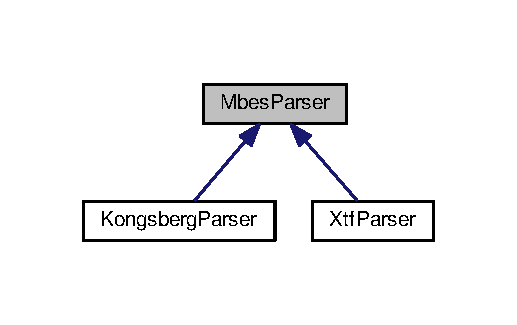
\includegraphics[width=248pt]{classMbesParser__inherit__graph}
\end{center}
\end{figure}
\subsection*{Fonctions membres publiques}
\begin{DoxyCompactItemize}
\item 
\hyperlink{classMbesParser_ac6ef7327a407484a528c0b1c0384db9f}{Mbes\+Parser} ()
\item 
virtual \hyperlink{classMbesParser_aa72a4049542622ecebba6aec01a1e763}{$\sim$\+Mbes\+Parser} ()
\item 
virtual void \hyperlink{classMbesParser_a10e172520c1ca2b87dab51aef9e57c2a}{parse} (std\+::string filename)
\item 
virtual void \hyperlink{classMbesParser_a347e78a8a1369c1ea6e63e7eea474b31}{process\+Attitude} (uint64\+\_\+t micro\+Epoch, double heading, double pitch, double roll)
\item 
virtual void \hyperlink{classMbesParser_add86a02726482d3a8e2a8aaf7f4beefa}{process\+Position} (uint64\+\_\+t micro\+Epoch, double longitude, double latitude, double height)
\item 
virtual void \hyperlink{classMbesParser_a9c099ea1003fff3c99991c37da1d40a6}{process\+Ping} (uint64\+\_\+t micro\+Epoch, long id, double beam\+Angle, double tilt\+Angle, double two\+Way\+Travel\+Time, uint32\+\_\+t quality, uint32\+\_\+t intensity)
\item 
virtual void \hyperlink{classMbesParser_ab6481abeb95b37b435a3bf2d705eba19}{process\+Swath\+Start} ()
\end{DoxyCompactItemize}


\subsection{Documentation des constructeurs et destructeur}
\mbox{\Hypertarget{classMbesParser_ac6ef7327a407484a528c0b1c0384db9f}\label{classMbesParser_ac6ef7327a407484a528c0b1c0384db9f}} 
\index{Mbes\+Parser@{Mbes\+Parser}!Mbes\+Parser@{Mbes\+Parser}}
\index{Mbes\+Parser@{Mbes\+Parser}!Mbes\+Parser@{Mbes\+Parser}}
\subsubsection{\texorpdfstring{Mbes\+Parser()}{MbesParser()}}
{\footnotesize\ttfamily Mbes\+Parser\+::\+Mbes\+Parser (\begin{DoxyParamCaption}{ }\end{DoxyParamCaption})}

\mbox{\Hypertarget{classMbesParser_aa72a4049542622ecebba6aec01a1e763}\label{classMbesParser_aa72a4049542622ecebba6aec01a1e763}} 
\index{Mbes\+Parser@{Mbes\+Parser}!````~Mbes\+Parser@{$\sim$\+Mbes\+Parser}}
\index{````~Mbes\+Parser@{$\sim$\+Mbes\+Parser}!Mbes\+Parser@{Mbes\+Parser}}
\subsubsection{\texorpdfstring{$\sim$\+Mbes\+Parser()}{~MbesParser()}}
{\footnotesize\ttfamily virtual Mbes\+Parser\+::$\sim$\+Mbes\+Parser (\begin{DoxyParamCaption}{ }\end{DoxyParamCaption})\hspace{0.3cm}{\ttfamily [inline]}, {\ttfamily [virtual]}}



\subsection{Documentation des fonctions membres}
\mbox{\Hypertarget{classMbesParser_a10e172520c1ca2b87dab51aef9e57c2a}\label{classMbesParser_a10e172520c1ca2b87dab51aef9e57c2a}} 
\index{Mbes\+Parser@{Mbes\+Parser}!parse@{parse}}
\index{parse@{parse}!Mbes\+Parser@{Mbes\+Parser}}
\subsubsection{\texorpdfstring{parse()}{parse()}}
{\footnotesize\ttfamily virtual void Mbes\+Parser\+::parse (\begin{DoxyParamCaption}\item[{std\+::string}]{filename }\end{DoxyParamCaption})\hspace{0.3cm}{\ttfamily [inline]}, {\ttfamily [virtual]}}



Réimplémentée dans \hyperlink{classKongsbergParser_af7c31817a75fc4d153945f35f08b9d99}{Kongsberg\+Parser}.

\mbox{\Hypertarget{classMbesParser_a347e78a8a1369c1ea6e63e7eea474b31}\label{classMbesParser_a347e78a8a1369c1ea6e63e7eea474b31}} 
\index{Mbes\+Parser@{Mbes\+Parser}!process\+Attitude@{process\+Attitude}}
\index{process\+Attitude@{process\+Attitude}!Mbes\+Parser@{Mbes\+Parser}}
\subsubsection{\texorpdfstring{process\+Attitude()}{processAttitude()}}
{\footnotesize\ttfamily virtual void Mbes\+Parser\+::process\+Attitude (\begin{DoxyParamCaption}\item[{uint64\+\_\+t}]{micro\+Epoch,  }\item[{double}]{heading,  }\item[{double}]{pitch,  }\item[{double}]{roll }\end{DoxyParamCaption})\hspace{0.3cm}{\ttfamily [inline]}, {\ttfamily [virtual]}}



Réimplémentée dans \hyperlink{classKongsbergParser_aa241961b762eb4fed4702a337573d46d}{Kongsberg\+Parser}.

\mbox{\Hypertarget{classMbesParser_a9c099ea1003fff3c99991c37da1d40a6}\label{classMbesParser_a9c099ea1003fff3c99991c37da1d40a6}} 
\index{Mbes\+Parser@{Mbes\+Parser}!process\+Ping@{process\+Ping}}
\index{process\+Ping@{process\+Ping}!Mbes\+Parser@{Mbes\+Parser}}
\subsubsection{\texorpdfstring{process\+Ping()}{processPing()}}
{\footnotesize\ttfamily virtual void Mbes\+Parser\+::process\+Ping (\begin{DoxyParamCaption}\item[{uint64\+\_\+t}]{micro\+Epoch,  }\item[{long}]{id,  }\item[{double}]{beam\+Angle,  }\item[{double}]{tilt\+Angle,  }\item[{double}]{two\+Way\+Travel\+Time,  }\item[{uint32\+\_\+t}]{quality,  }\item[{uint32\+\_\+t}]{intensity }\end{DoxyParamCaption})\hspace{0.3cm}{\ttfamily [inline]}, {\ttfamily [virtual]}}



Réimplémentée dans \hyperlink{classXtfParser_ae8932c52b4030f14acd8b4419037c3eb}{Xtf\+Parser}.

\mbox{\Hypertarget{classMbesParser_add86a02726482d3a8e2a8aaf7f4beefa}\label{classMbesParser_add86a02726482d3a8e2a8aaf7f4beefa}} 
\index{Mbes\+Parser@{Mbes\+Parser}!process\+Position@{process\+Position}}
\index{process\+Position@{process\+Position}!Mbes\+Parser@{Mbes\+Parser}}
\subsubsection{\texorpdfstring{process\+Position()}{processPosition()}}
{\footnotesize\ttfamily virtual void Mbes\+Parser\+::process\+Position (\begin{DoxyParamCaption}\item[{uint64\+\_\+t}]{micro\+Epoch,  }\item[{double}]{longitude,  }\item[{double}]{latitude,  }\item[{double}]{height }\end{DoxyParamCaption})\hspace{0.3cm}{\ttfamily [inline]}, {\ttfamily [virtual]}}



Réimplémentée dans \hyperlink{classKongsbergParser_a692580461f3e6d8f822cb84cf3ed6a3c}{Kongsberg\+Parser}, et \hyperlink{classXtfParser_abbb02ef84a6f01696fb1f6ed23d2bb5f}{Xtf\+Parser}.

\mbox{\Hypertarget{classMbesParser_ab6481abeb95b37b435a3bf2d705eba19}\label{classMbesParser_ab6481abeb95b37b435a3bf2d705eba19}} 
\index{Mbes\+Parser@{Mbes\+Parser}!process\+Swath\+Start@{process\+Swath\+Start}}
\index{process\+Swath\+Start@{process\+Swath\+Start}!Mbes\+Parser@{Mbes\+Parser}}
\subsubsection{\texorpdfstring{process\+Swath\+Start()}{processSwathStart()}}
{\footnotesize\ttfamily virtual void Mbes\+Parser\+::process\+Swath\+Start (\begin{DoxyParamCaption}{ }\end{DoxyParamCaption})\hspace{0.3cm}{\ttfamily [inline]}, {\ttfamily [virtual]}}



La documentation de cette classe a été générée à partir du fichier suivant \+:\begin{DoxyCompactItemize}
\item 
src/datagrams/\hyperlink{MbesParser_8hpp}{Mbes\+Parser.\+hpp}\end{DoxyCompactItemize}

\hypertarget{classNmeaUtils}{}\section{Référence de la classe Nmea\+Utils}
\label{classNmeaUtils}\index{Nmea\+Utils@{Nmea\+Utils}}


{\ttfamily \#include $<$Nmea\+Utils.\+hpp$>$}

\subsection*{Fonctions membres publiques statiques}
\begin{DoxyCompactItemize}
\item 
static double \hyperlink{classNmeaUtils_a35921c270ebfc026fd911ad8c18e8328}{extract\+Height\+From\+G\+GK} (std\+::string \&ggk\+String)
\begin{DoxyCompactList}\small\item\em extract\+Height\+From\+G\+GK Extracts ellipsoidal height from G\+GK \end{DoxyCompactList}\item 
static double \hyperlink{classNmeaUtils_a93ff32d3b56b1f032d801df2763d4f22}{extract\+Height\+From\+G\+GA} (std\+::string \&gga\+String)
\begin{DoxyCompactList}\small\item\em extract\+Height\+From\+G\+GA Extracts ellipsoidal height from G\+GA \end{DoxyCompactList}\end{DoxyCompactItemize}


\subsection{Documentation des fonctions membres}
\mbox{\Hypertarget{classNmeaUtils_a93ff32d3b56b1f032d801df2763d4f22}\label{classNmeaUtils_a93ff32d3b56b1f032d801df2763d4f22}} 
\index{Nmea\+Utils@{Nmea\+Utils}!extract\+Height\+From\+G\+GA@{extract\+Height\+From\+G\+GA}}
\index{extract\+Height\+From\+G\+GA@{extract\+Height\+From\+G\+GA}!Nmea\+Utils@{Nmea\+Utils}}
\subsubsection{\texorpdfstring{extract\+Height\+From\+G\+G\+A()}{extractHeightFromGGA()}}
{\footnotesize\ttfamily double Nmea\+Utils\+::extract\+Height\+From\+G\+GA (\begin{DoxyParamCaption}\item[{std\+::string \&}]{gga\+String }\end{DoxyParamCaption})\hspace{0.3cm}{\ttfamily [static]}}



extract\+Height\+From\+G\+GA Extracts ellipsoidal height from G\+GA 


\begin{DoxyParams}{Paramètres}
{\em gga\+String} & \\
\hline
\end{DoxyParams}
\begin{DoxyReturn}{Renvoie}

\end{DoxyReturn}
\mbox{\Hypertarget{classNmeaUtils_a35921c270ebfc026fd911ad8c18e8328}\label{classNmeaUtils_a35921c270ebfc026fd911ad8c18e8328}} 
\index{Nmea\+Utils@{Nmea\+Utils}!extract\+Height\+From\+G\+GK@{extract\+Height\+From\+G\+GK}}
\index{extract\+Height\+From\+G\+GK@{extract\+Height\+From\+G\+GK}!Nmea\+Utils@{Nmea\+Utils}}
\subsubsection{\texorpdfstring{extract\+Height\+From\+G\+G\+K()}{extractHeightFromGGK()}}
{\footnotesize\ttfamily double Nmea\+Utils\+::extract\+Height\+From\+G\+GK (\begin{DoxyParamCaption}\item[{std\+::string \&}]{ggk\+String }\end{DoxyParamCaption})\hspace{0.3cm}{\ttfamily [static]}}



extract\+Height\+From\+G\+GK Extracts ellipsoidal height from G\+GK 


\begin{DoxyParams}{Paramètres}
{\em ggk\+String} & \\
\hline
\end{DoxyParams}
\begin{DoxyReturn}{Renvoie}

\end{DoxyReturn}


La documentation de cette classe a été générée à partir du fichier suivant \+:\begin{DoxyCompactItemize}
\item 
src/utils/\hyperlink{NmeaUtils_8hpp}{Nmea\+Utils.\+hpp}\end{DoxyCompactItemize}

\hypertarget{structSNP0}{}\section{Référence de la structure S\+N\+P0}
\label{structSNP0}\index{S\+N\+P0@{S\+N\+P0}}


{\ttfamily \#include $<$Xtf\+Types.\+hpp$>$}

\subsection*{Attributs publics}
\begin{DoxyCompactItemize}
\item 
uint32\+\_\+t \hyperlink{structSNP0_ab0014708aadf0ad4b1a26ccef2191c24}{Id}
\item 
uint16\+\_\+t \hyperlink{structSNP0_a948d2af915700abd82c6c725da30c8a2}{Header\+Size}
\item 
uint16\+\_\+t \hyperlink{structSNP0_a40fa21d4ffa7a3e3beb0bc1c863eaa93}{Data\+Size}
\item 
uint32\+\_\+t \hyperlink{structSNP0_aea1f45b21957092849539ae85caeabba}{Ping\+Number}
\item 
uint32\+\_\+t \hyperlink{structSNP0_a0e5af36fb4c4a7ad4991d0fee39849f0}{Seconds}
\item 
uint32\+\_\+t \hyperlink{structSNP0_afd37fe6d7e52b61a9d011902b6742c19}{Millisec}
\item 
uint16\+\_\+t \hyperlink{structSNP0_af63465612e6fbbbd00438aa4fd407111}{Latency}
\item 
uint16\+\_\+t \hyperlink{structSNP0_ae80fe309155e6ca399ad5d4e3eb71ad9}{Sonar\+ID} \mbox{[}2\mbox{]}
\item 
uint16\+\_\+t \hyperlink{structSNP0_ad140e764420ebcdfdfe86e6b22045d70}{Sonar\+Model}
\item 
uint16\+\_\+t \hyperlink{structSNP0_a20f0a2401ebc774d708b7bbfaf9a891f}{Frequency}
\item 
uint16\+\_\+t \hyperlink{structSNP0_a34acd7f87f72ec98e040260e54fac986}{S\+Speed}
\item 
uint16\+\_\+t \hyperlink{structSNP0_aa2d1893b43ba99412fcf0c8a84f70e2b}{Sample\+Rate}
\item 
uint16\+\_\+t \hyperlink{structSNP0_a896fe8fc11f848e0e8fe1cb07ec465d2}{Ping\+Rate}
\item 
uint16\+\_\+t \hyperlink{structSNP0_ac2fa52ce9ce23989f60a52eea9570f8e}{Range}
\item 
uint16\+\_\+t \hyperlink{structSNP0_a1ee6f80141df06590712bc77aa6dcb85}{Power}
\item 
uint16\+\_\+t \hyperlink{structSNP0_aba161dd31bd98e9cc88304d1b227c6fb}{Gain}
\item 
uint16\+\_\+t \hyperlink{structSNP0_a56e19234d0745ef534a29bd314114dd1}{Pulse\+Width}
\item 
uint16\+\_\+t \hyperlink{structSNP0_abf8caba4fc96eec014c47047358d7727}{Spread}
\item 
uint16\+\_\+t \hyperlink{structSNP0_ac1b74212076ec40d2652abdff2ce2ad3}{Absorb}
\item 
uint16\+\_\+t \hyperlink{structSNP0_ab5b89bdac9c2bd9fdf71ab133ad53552}{Proj}
\item 
uint16\+\_\+t \hyperlink{structSNP0_a33535554e463b4cc78628e37b1acd0c4}{Proj\+Width}
\item 
uint16\+\_\+t \hyperlink{structSNP0_a2147bcebb42440050366b57709ad53e5}{Spacing\+Num}
\item 
uint16\+\_\+t \hyperlink{structSNP0_aaa687482640087e282cf75e26ee67d83}{Spacing\+Den}
\item 
int16\+\_\+t \hyperlink{structSNP0_a020495ec71e847c17c02a3643df5829b}{Proj\+Angle}
\item 
uint16\+\_\+t \hyperlink{structSNP0_a671b6f588d5aecfd2b9001899bcd9fff}{Min\+Range}
\item 
uint16\+\_\+t \hyperlink{structSNP0_ab4fe2a839a62b29dfd787fdc096d7948}{Max\+Range}
\item 
uint16\+\_\+t \hyperlink{structSNP0_aae9f0a30189d0282fc71c2b0f3ac2115}{Min\+Depth}
\item 
uint16\+\_\+t \hyperlink{structSNP0_abaaecae3da038633e9d1833699789632}{Max\+Depth}
\item 
uint16\+\_\+t \hyperlink{structSNP0_a5e467787df838b60faa5094f7348633e}{Filters}
\item 
uint8\+\_\+t \hyperlink{structSNP0_a57fc117609cb0851f2e09fe313605eb4}{b\+Flags} \mbox{[}2\mbox{]}
\item 
int16\+\_\+t \hyperlink{structSNP0_a0bc29ffc0f2d8ea4cceb392429fab0e3}{Head\+Temp}
\item 
uint16\+\_\+t \hyperlink{structSNP0_a801bf122ae734d79fe78d65b7a007f87}{Beam\+Cnt}
\end{DoxyCompactItemize}


\subsection{Documentation des données membres}
\mbox{\Hypertarget{structSNP0_ac1b74212076ec40d2652abdff2ce2ad3}\label{structSNP0_ac1b74212076ec40d2652abdff2ce2ad3}} 
\index{S\+N\+P0@{S\+N\+P0}!Absorb@{Absorb}}
\index{Absorb@{Absorb}!S\+N\+P0@{S\+N\+P0}}
\subsubsection{\texorpdfstring{Absorb}{Absorb}}
{\footnotesize\ttfamily uint16\+\_\+t S\+N\+P0\+::\+Absorb}

\mbox{\Hypertarget{structSNP0_a801bf122ae734d79fe78d65b7a007f87}\label{structSNP0_a801bf122ae734d79fe78d65b7a007f87}} 
\index{S\+N\+P0@{S\+N\+P0}!Beam\+Cnt@{Beam\+Cnt}}
\index{Beam\+Cnt@{Beam\+Cnt}!S\+N\+P0@{S\+N\+P0}}
\subsubsection{\texorpdfstring{Beam\+Cnt}{BeamCnt}}
{\footnotesize\ttfamily uint16\+\_\+t S\+N\+P0\+::\+Beam\+Cnt}

\mbox{\Hypertarget{structSNP0_a57fc117609cb0851f2e09fe313605eb4}\label{structSNP0_a57fc117609cb0851f2e09fe313605eb4}} 
\index{S\+N\+P0@{S\+N\+P0}!b\+Flags@{b\+Flags}}
\index{b\+Flags@{b\+Flags}!S\+N\+P0@{S\+N\+P0}}
\subsubsection{\texorpdfstring{b\+Flags}{bFlags}}
{\footnotesize\ttfamily uint8\+\_\+t S\+N\+P0\+::b\+Flags\mbox{[}2\mbox{]}}

\mbox{\Hypertarget{structSNP0_a40fa21d4ffa7a3e3beb0bc1c863eaa93}\label{structSNP0_a40fa21d4ffa7a3e3beb0bc1c863eaa93}} 
\index{S\+N\+P0@{S\+N\+P0}!Data\+Size@{Data\+Size}}
\index{Data\+Size@{Data\+Size}!S\+N\+P0@{S\+N\+P0}}
\subsubsection{\texorpdfstring{Data\+Size}{DataSize}}
{\footnotesize\ttfamily uint16\+\_\+t S\+N\+P0\+::\+Data\+Size}

\mbox{\Hypertarget{structSNP0_a5e467787df838b60faa5094f7348633e}\label{structSNP0_a5e467787df838b60faa5094f7348633e}} 
\index{S\+N\+P0@{S\+N\+P0}!Filters@{Filters}}
\index{Filters@{Filters}!S\+N\+P0@{S\+N\+P0}}
\subsubsection{\texorpdfstring{Filters}{Filters}}
{\footnotesize\ttfamily uint16\+\_\+t S\+N\+P0\+::\+Filters}

\mbox{\Hypertarget{structSNP0_a20f0a2401ebc774d708b7bbfaf9a891f}\label{structSNP0_a20f0a2401ebc774d708b7bbfaf9a891f}} 
\index{S\+N\+P0@{S\+N\+P0}!Frequency@{Frequency}}
\index{Frequency@{Frequency}!S\+N\+P0@{S\+N\+P0}}
\subsubsection{\texorpdfstring{Frequency}{Frequency}}
{\footnotesize\ttfamily uint16\+\_\+t S\+N\+P0\+::\+Frequency}

\mbox{\Hypertarget{structSNP0_aba161dd31bd98e9cc88304d1b227c6fb}\label{structSNP0_aba161dd31bd98e9cc88304d1b227c6fb}} 
\index{S\+N\+P0@{S\+N\+P0}!Gain@{Gain}}
\index{Gain@{Gain}!S\+N\+P0@{S\+N\+P0}}
\subsubsection{\texorpdfstring{Gain}{Gain}}
{\footnotesize\ttfamily uint16\+\_\+t S\+N\+P0\+::\+Gain}

\mbox{\Hypertarget{structSNP0_a948d2af915700abd82c6c725da30c8a2}\label{structSNP0_a948d2af915700abd82c6c725da30c8a2}} 
\index{S\+N\+P0@{S\+N\+P0}!Header\+Size@{Header\+Size}}
\index{Header\+Size@{Header\+Size}!S\+N\+P0@{S\+N\+P0}}
\subsubsection{\texorpdfstring{Header\+Size}{HeaderSize}}
{\footnotesize\ttfamily uint16\+\_\+t S\+N\+P0\+::\+Header\+Size}

\mbox{\Hypertarget{structSNP0_a0bc29ffc0f2d8ea4cceb392429fab0e3}\label{structSNP0_a0bc29ffc0f2d8ea4cceb392429fab0e3}} 
\index{S\+N\+P0@{S\+N\+P0}!Head\+Temp@{Head\+Temp}}
\index{Head\+Temp@{Head\+Temp}!S\+N\+P0@{S\+N\+P0}}
\subsubsection{\texorpdfstring{Head\+Temp}{HeadTemp}}
{\footnotesize\ttfamily int16\+\_\+t S\+N\+P0\+::\+Head\+Temp}

\mbox{\Hypertarget{structSNP0_ab0014708aadf0ad4b1a26ccef2191c24}\label{structSNP0_ab0014708aadf0ad4b1a26ccef2191c24}} 
\index{S\+N\+P0@{S\+N\+P0}!Id@{Id}}
\index{Id@{Id}!S\+N\+P0@{S\+N\+P0}}
\subsubsection{\texorpdfstring{Id}{Id}}
{\footnotesize\ttfamily uint32\+\_\+t S\+N\+P0\+::\+Id}

\mbox{\Hypertarget{structSNP0_af63465612e6fbbbd00438aa4fd407111}\label{structSNP0_af63465612e6fbbbd00438aa4fd407111}} 
\index{S\+N\+P0@{S\+N\+P0}!Latency@{Latency}}
\index{Latency@{Latency}!S\+N\+P0@{S\+N\+P0}}
\subsubsection{\texorpdfstring{Latency}{Latency}}
{\footnotesize\ttfamily uint16\+\_\+t S\+N\+P0\+::\+Latency}

\mbox{\Hypertarget{structSNP0_abaaecae3da038633e9d1833699789632}\label{structSNP0_abaaecae3da038633e9d1833699789632}} 
\index{S\+N\+P0@{S\+N\+P0}!Max\+Depth@{Max\+Depth}}
\index{Max\+Depth@{Max\+Depth}!S\+N\+P0@{S\+N\+P0}}
\subsubsection{\texorpdfstring{Max\+Depth}{MaxDepth}}
{\footnotesize\ttfamily uint16\+\_\+t S\+N\+P0\+::\+Max\+Depth}

\mbox{\Hypertarget{structSNP0_ab4fe2a839a62b29dfd787fdc096d7948}\label{structSNP0_ab4fe2a839a62b29dfd787fdc096d7948}} 
\index{S\+N\+P0@{S\+N\+P0}!Max\+Range@{Max\+Range}}
\index{Max\+Range@{Max\+Range}!S\+N\+P0@{S\+N\+P0}}
\subsubsection{\texorpdfstring{Max\+Range}{MaxRange}}
{\footnotesize\ttfamily uint16\+\_\+t S\+N\+P0\+::\+Max\+Range}

\mbox{\Hypertarget{structSNP0_afd37fe6d7e52b61a9d011902b6742c19}\label{structSNP0_afd37fe6d7e52b61a9d011902b6742c19}} 
\index{S\+N\+P0@{S\+N\+P0}!Millisec@{Millisec}}
\index{Millisec@{Millisec}!S\+N\+P0@{S\+N\+P0}}
\subsubsection{\texorpdfstring{Millisec}{Millisec}}
{\footnotesize\ttfamily uint32\+\_\+t S\+N\+P0\+::\+Millisec}

\mbox{\Hypertarget{structSNP0_aae9f0a30189d0282fc71c2b0f3ac2115}\label{structSNP0_aae9f0a30189d0282fc71c2b0f3ac2115}} 
\index{S\+N\+P0@{S\+N\+P0}!Min\+Depth@{Min\+Depth}}
\index{Min\+Depth@{Min\+Depth}!S\+N\+P0@{S\+N\+P0}}
\subsubsection{\texorpdfstring{Min\+Depth}{MinDepth}}
{\footnotesize\ttfamily uint16\+\_\+t S\+N\+P0\+::\+Min\+Depth}

\mbox{\Hypertarget{structSNP0_a671b6f588d5aecfd2b9001899bcd9fff}\label{structSNP0_a671b6f588d5aecfd2b9001899bcd9fff}} 
\index{S\+N\+P0@{S\+N\+P0}!Min\+Range@{Min\+Range}}
\index{Min\+Range@{Min\+Range}!S\+N\+P0@{S\+N\+P0}}
\subsubsection{\texorpdfstring{Min\+Range}{MinRange}}
{\footnotesize\ttfamily uint16\+\_\+t S\+N\+P0\+::\+Min\+Range}

\mbox{\Hypertarget{structSNP0_aea1f45b21957092849539ae85caeabba}\label{structSNP0_aea1f45b21957092849539ae85caeabba}} 
\index{S\+N\+P0@{S\+N\+P0}!Ping\+Number@{Ping\+Number}}
\index{Ping\+Number@{Ping\+Number}!S\+N\+P0@{S\+N\+P0}}
\subsubsection{\texorpdfstring{Ping\+Number}{PingNumber}}
{\footnotesize\ttfamily uint32\+\_\+t S\+N\+P0\+::\+Ping\+Number}

\mbox{\Hypertarget{structSNP0_a896fe8fc11f848e0e8fe1cb07ec465d2}\label{structSNP0_a896fe8fc11f848e0e8fe1cb07ec465d2}} 
\index{S\+N\+P0@{S\+N\+P0}!Ping\+Rate@{Ping\+Rate}}
\index{Ping\+Rate@{Ping\+Rate}!S\+N\+P0@{S\+N\+P0}}
\subsubsection{\texorpdfstring{Ping\+Rate}{PingRate}}
{\footnotesize\ttfamily uint16\+\_\+t S\+N\+P0\+::\+Ping\+Rate}

\mbox{\Hypertarget{structSNP0_a1ee6f80141df06590712bc77aa6dcb85}\label{structSNP0_a1ee6f80141df06590712bc77aa6dcb85}} 
\index{S\+N\+P0@{S\+N\+P0}!Power@{Power}}
\index{Power@{Power}!S\+N\+P0@{S\+N\+P0}}
\subsubsection{\texorpdfstring{Power}{Power}}
{\footnotesize\ttfamily uint16\+\_\+t S\+N\+P0\+::\+Power}

\mbox{\Hypertarget{structSNP0_ab5b89bdac9c2bd9fdf71ab133ad53552}\label{structSNP0_ab5b89bdac9c2bd9fdf71ab133ad53552}} 
\index{S\+N\+P0@{S\+N\+P0}!Proj@{Proj}}
\index{Proj@{Proj}!S\+N\+P0@{S\+N\+P0}}
\subsubsection{\texorpdfstring{Proj}{Proj}}
{\footnotesize\ttfamily uint16\+\_\+t S\+N\+P0\+::\+Proj}

\mbox{\Hypertarget{structSNP0_a020495ec71e847c17c02a3643df5829b}\label{structSNP0_a020495ec71e847c17c02a3643df5829b}} 
\index{S\+N\+P0@{S\+N\+P0}!Proj\+Angle@{Proj\+Angle}}
\index{Proj\+Angle@{Proj\+Angle}!S\+N\+P0@{S\+N\+P0}}
\subsubsection{\texorpdfstring{Proj\+Angle}{ProjAngle}}
{\footnotesize\ttfamily int16\+\_\+t S\+N\+P0\+::\+Proj\+Angle}

\mbox{\Hypertarget{structSNP0_a33535554e463b4cc78628e37b1acd0c4}\label{structSNP0_a33535554e463b4cc78628e37b1acd0c4}} 
\index{S\+N\+P0@{S\+N\+P0}!Proj\+Width@{Proj\+Width}}
\index{Proj\+Width@{Proj\+Width}!S\+N\+P0@{S\+N\+P0}}
\subsubsection{\texorpdfstring{Proj\+Width}{ProjWidth}}
{\footnotesize\ttfamily uint16\+\_\+t S\+N\+P0\+::\+Proj\+Width}

\mbox{\Hypertarget{structSNP0_a56e19234d0745ef534a29bd314114dd1}\label{structSNP0_a56e19234d0745ef534a29bd314114dd1}} 
\index{S\+N\+P0@{S\+N\+P0}!Pulse\+Width@{Pulse\+Width}}
\index{Pulse\+Width@{Pulse\+Width}!S\+N\+P0@{S\+N\+P0}}
\subsubsection{\texorpdfstring{Pulse\+Width}{PulseWidth}}
{\footnotesize\ttfamily uint16\+\_\+t S\+N\+P0\+::\+Pulse\+Width}

\mbox{\Hypertarget{structSNP0_ac2fa52ce9ce23989f60a52eea9570f8e}\label{structSNP0_ac2fa52ce9ce23989f60a52eea9570f8e}} 
\index{S\+N\+P0@{S\+N\+P0}!Range@{Range}}
\index{Range@{Range}!S\+N\+P0@{S\+N\+P0}}
\subsubsection{\texorpdfstring{Range}{Range}}
{\footnotesize\ttfamily uint16\+\_\+t S\+N\+P0\+::\+Range}

\mbox{\Hypertarget{structSNP0_aa2d1893b43ba99412fcf0c8a84f70e2b}\label{structSNP0_aa2d1893b43ba99412fcf0c8a84f70e2b}} 
\index{S\+N\+P0@{S\+N\+P0}!Sample\+Rate@{Sample\+Rate}}
\index{Sample\+Rate@{Sample\+Rate}!S\+N\+P0@{S\+N\+P0}}
\subsubsection{\texorpdfstring{Sample\+Rate}{SampleRate}}
{\footnotesize\ttfamily uint16\+\_\+t S\+N\+P0\+::\+Sample\+Rate}

\mbox{\Hypertarget{structSNP0_a0e5af36fb4c4a7ad4991d0fee39849f0}\label{structSNP0_a0e5af36fb4c4a7ad4991d0fee39849f0}} 
\index{S\+N\+P0@{S\+N\+P0}!Seconds@{Seconds}}
\index{Seconds@{Seconds}!S\+N\+P0@{S\+N\+P0}}
\subsubsection{\texorpdfstring{Seconds}{Seconds}}
{\footnotesize\ttfamily uint32\+\_\+t S\+N\+P0\+::\+Seconds}

\mbox{\Hypertarget{structSNP0_ae80fe309155e6ca399ad5d4e3eb71ad9}\label{structSNP0_ae80fe309155e6ca399ad5d4e3eb71ad9}} 
\index{S\+N\+P0@{S\+N\+P0}!Sonar\+ID@{Sonar\+ID}}
\index{Sonar\+ID@{Sonar\+ID}!S\+N\+P0@{S\+N\+P0}}
\subsubsection{\texorpdfstring{Sonar\+ID}{SonarID}}
{\footnotesize\ttfamily uint16\+\_\+t S\+N\+P0\+::\+Sonar\+ID\mbox{[}2\mbox{]}}

\mbox{\Hypertarget{structSNP0_ad140e764420ebcdfdfe86e6b22045d70}\label{structSNP0_ad140e764420ebcdfdfe86e6b22045d70}} 
\index{S\+N\+P0@{S\+N\+P0}!Sonar\+Model@{Sonar\+Model}}
\index{Sonar\+Model@{Sonar\+Model}!S\+N\+P0@{S\+N\+P0}}
\subsubsection{\texorpdfstring{Sonar\+Model}{SonarModel}}
{\footnotesize\ttfamily uint16\+\_\+t S\+N\+P0\+::\+Sonar\+Model}

\mbox{\Hypertarget{structSNP0_aaa687482640087e282cf75e26ee67d83}\label{structSNP0_aaa687482640087e282cf75e26ee67d83}} 
\index{S\+N\+P0@{S\+N\+P0}!Spacing\+Den@{Spacing\+Den}}
\index{Spacing\+Den@{Spacing\+Den}!S\+N\+P0@{S\+N\+P0}}
\subsubsection{\texorpdfstring{Spacing\+Den}{SpacingDen}}
{\footnotesize\ttfamily uint16\+\_\+t S\+N\+P0\+::\+Spacing\+Den}

\mbox{\Hypertarget{structSNP0_a2147bcebb42440050366b57709ad53e5}\label{structSNP0_a2147bcebb42440050366b57709ad53e5}} 
\index{S\+N\+P0@{S\+N\+P0}!Spacing\+Num@{Spacing\+Num}}
\index{Spacing\+Num@{Spacing\+Num}!S\+N\+P0@{S\+N\+P0}}
\subsubsection{\texorpdfstring{Spacing\+Num}{SpacingNum}}
{\footnotesize\ttfamily uint16\+\_\+t S\+N\+P0\+::\+Spacing\+Num}

\mbox{\Hypertarget{structSNP0_abf8caba4fc96eec014c47047358d7727}\label{structSNP0_abf8caba4fc96eec014c47047358d7727}} 
\index{S\+N\+P0@{S\+N\+P0}!Spread@{Spread}}
\index{Spread@{Spread}!S\+N\+P0@{S\+N\+P0}}
\subsubsection{\texorpdfstring{Spread}{Spread}}
{\footnotesize\ttfamily uint16\+\_\+t S\+N\+P0\+::\+Spread}

\mbox{\Hypertarget{structSNP0_a34acd7f87f72ec98e040260e54fac986}\label{structSNP0_a34acd7f87f72ec98e040260e54fac986}} 
\index{S\+N\+P0@{S\+N\+P0}!S\+Speed@{S\+Speed}}
\index{S\+Speed@{S\+Speed}!S\+N\+P0@{S\+N\+P0}}
\subsubsection{\texorpdfstring{S\+Speed}{SSpeed}}
{\footnotesize\ttfamily uint16\+\_\+t S\+N\+P0\+::\+S\+Speed}



La documentation de cette structure a été générée à partir du fichier suivant \+:\begin{DoxyCompactItemize}
\item 
src/datagrams/xtf/\hyperlink{XtfTypes_8hpp}{Xtf\+Types.\+hpp}\end{DoxyCompactItemize}

\hypertarget{structSNP1}{}\section{Référence de la structure S\+N\+P1}
\label{structSNP1}\index{S\+N\+P1@{S\+N\+P1}}


{\ttfamily \#include $<$Xtf\+Types.\+hpp$>$}

\subsection*{Attributs publics}
\begin{DoxyCompactItemize}
\item 
uint32\+\_\+t \hyperlink{structSNP1_ae831f0f3db4684dc376a024baeb78177}{ID}
\item 
uint16\+\_\+t \hyperlink{structSNP1_adbfcf4adc5b40b66c93b6ba29614e676}{Header\+Size}
\item 
uint16\+\_\+t \hyperlink{structSNP1_a410d96cbff9feb7a9a86dd79db7f3222}{Data\+Size}
\item 
uint32\+\_\+t \hyperlink{structSNP1_acf218e8c904b3fd1070a2d1953fbab97}{Ping\+Number}
\item 
uint16\+\_\+t \hyperlink{structSNP1_ade91373e79d5eb32e5a0bbb8b9832b72}{Beam}
\item 
uint16\+\_\+t \hyperlink{structSNP1_a56b038e82536d0cd2f6f65dac10b76aa}{Snip\+Samples}
\item 
uint16\+\_\+t \hyperlink{structSNP1_a7143f99165c37cbb26caa5c92955f1fa}{Gain\+Start}
\item 
uint16\+\_\+t \hyperlink{structSNP1_ade59225835d0a113e80f1d1f3f2f00e4}{Gain\+End}
\item 
uint16\+\_\+t \hyperlink{structSNP1_a2bcf51d775dc18ca4dac4920215770ca}{Frag\+Offset}
\item 
uint16\+\_\+t \hyperlink{structSNP1_a2568a5fb3306a9fd1f5fad4f11430676}{Frag\+Samples}
\end{DoxyCompactItemize}


\subsection{Documentation des données membres}
\mbox{\Hypertarget{structSNP1_ade91373e79d5eb32e5a0bbb8b9832b72}\label{structSNP1_ade91373e79d5eb32e5a0bbb8b9832b72}} 
\index{S\+N\+P1@{S\+N\+P1}!Beam@{Beam}}
\index{Beam@{Beam}!S\+N\+P1@{S\+N\+P1}}
\subsubsection{\texorpdfstring{Beam}{Beam}}
{\footnotesize\ttfamily uint16\+\_\+t S\+N\+P1\+::\+Beam}

\mbox{\Hypertarget{structSNP1_a410d96cbff9feb7a9a86dd79db7f3222}\label{structSNP1_a410d96cbff9feb7a9a86dd79db7f3222}} 
\index{S\+N\+P1@{S\+N\+P1}!Data\+Size@{Data\+Size}}
\index{Data\+Size@{Data\+Size}!S\+N\+P1@{S\+N\+P1}}
\subsubsection{\texorpdfstring{Data\+Size}{DataSize}}
{\footnotesize\ttfamily uint16\+\_\+t S\+N\+P1\+::\+Data\+Size}

\mbox{\Hypertarget{structSNP1_a2bcf51d775dc18ca4dac4920215770ca}\label{structSNP1_a2bcf51d775dc18ca4dac4920215770ca}} 
\index{S\+N\+P1@{S\+N\+P1}!Frag\+Offset@{Frag\+Offset}}
\index{Frag\+Offset@{Frag\+Offset}!S\+N\+P1@{S\+N\+P1}}
\subsubsection{\texorpdfstring{Frag\+Offset}{FragOffset}}
{\footnotesize\ttfamily uint16\+\_\+t S\+N\+P1\+::\+Frag\+Offset}

\mbox{\Hypertarget{structSNP1_a2568a5fb3306a9fd1f5fad4f11430676}\label{structSNP1_a2568a5fb3306a9fd1f5fad4f11430676}} 
\index{S\+N\+P1@{S\+N\+P1}!Frag\+Samples@{Frag\+Samples}}
\index{Frag\+Samples@{Frag\+Samples}!S\+N\+P1@{S\+N\+P1}}
\subsubsection{\texorpdfstring{Frag\+Samples}{FragSamples}}
{\footnotesize\ttfamily uint16\+\_\+t S\+N\+P1\+::\+Frag\+Samples}

\mbox{\Hypertarget{structSNP1_ade59225835d0a113e80f1d1f3f2f00e4}\label{structSNP1_ade59225835d0a113e80f1d1f3f2f00e4}} 
\index{S\+N\+P1@{S\+N\+P1}!Gain\+End@{Gain\+End}}
\index{Gain\+End@{Gain\+End}!S\+N\+P1@{S\+N\+P1}}
\subsubsection{\texorpdfstring{Gain\+End}{GainEnd}}
{\footnotesize\ttfamily uint16\+\_\+t S\+N\+P1\+::\+Gain\+End}

\mbox{\Hypertarget{structSNP1_a7143f99165c37cbb26caa5c92955f1fa}\label{structSNP1_a7143f99165c37cbb26caa5c92955f1fa}} 
\index{S\+N\+P1@{S\+N\+P1}!Gain\+Start@{Gain\+Start}}
\index{Gain\+Start@{Gain\+Start}!S\+N\+P1@{S\+N\+P1}}
\subsubsection{\texorpdfstring{Gain\+Start}{GainStart}}
{\footnotesize\ttfamily uint16\+\_\+t S\+N\+P1\+::\+Gain\+Start}

\mbox{\Hypertarget{structSNP1_adbfcf4adc5b40b66c93b6ba29614e676}\label{structSNP1_adbfcf4adc5b40b66c93b6ba29614e676}} 
\index{S\+N\+P1@{S\+N\+P1}!Header\+Size@{Header\+Size}}
\index{Header\+Size@{Header\+Size}!S\+N\+P1@{S\+N\+P1}}
\subsubsection{\texorpdfstring{Header\+Size}{HeaderSize}}
{\footnotesize\ttfamily uint16\+\_\+t S\+N\+P1\+::\+Header\+Size}

\mbox{\Hypertarget{structSNP1_ae831f0f3db4684dc376a024baeb78177}\label{structSNP1_ae831f0f3db4684dc376a024baeb78177}} 
\index{S\+N\+P1@{S\+N\+P1}!ID@{ID}}
\index{ID@{ID}!S\+N\+P1@{S\+N\+P1}}
\subsubsection{\texorpdfstring{ID}{ID}}
{\footnotesize\ttfamily uint32\+\_\+t S\+N\+P1\+::\+ID}

\mbox{\Hypertarget{structSNP1_acf218e8c904b3fd1070a2d1953fbab97}\label{structSNP1_acf218e8c904b3fd1070a2d1953fbab97}} 
\index{S\+N\+P1@{S\+N\+P1}!Ping\+Number@{Ping\+Number}}
\index{Ping\+Number@{Ping\+Number}!S\+N\+P1@{S\+N\+P1}}
\subsubsection{\texorpdfstring{Ping\+Number}{PingNumber}}
{\footnotesize\ttfamily uint32\+\_\+t S\+N\+P1\+::\+Ping\+Number}

\mbox{\Hypertarget{structSNP1_a56b038e82536d0cd2f6f65dac10b76aa}\label{structSNP1_a56b038e82536d0cd2f6f65dac10b76aa}} 
\index{S\+N\+P1@{S\+N\+P1}!Snip\+Samples@{Snip\+Samples}}
\index{Snip\+Samples@{Snip\+Samples}!S\+N\+P1@{S\+N\+P1}}
\subsubsection{\texorpdfstring{Snip\+Samples}{SnipSamples}}
{\footnotesize\ttfamily uint16\+\_\+t S\+N\+P1\+::\+Snip\+Samples}



La documentation de cette structure a été générée à partir du fichier suivant \+:\begin{DoxyCompactItemize}
\item 
src/datagrams/xtf/\hyperlink{XtfTypes_8hpp}{Xtf\+Types.\+hpp}\end{DoxyCompactItemize}

\hypertarget{structXtfAttitudeData}{}\section{Référence de la structure Xtf\+Attitude\+Data}
\label{structXtfAttitudeData}\index{Xtf\+Attitude\+Data@{Xtf\+Attitude\+Data}}


{\ttfamily \#include $<$Xtf\+Types.\+hpp$>$}

\subsection*{Attributs publics}
\begin{DoxyCompactItemize}
\item 
uint32\+\_\+t \hyperlink{structXtfAttitudeData_a4d7429c51fbd9386ad742862f629bf4d}{Reserved2} \mbox{[}2\mbox{]}
\item 
uint32\+\_\+t \hyperlink{structXtfAttitudeData_ae30d080da0e06e1f781e333790a9bbed}{Epoch\+Microseconds}
\item 
uint32\+\_\+t \hyperlink{structXtfAttitudeData_aba5b0d9369962e937c499352401c0aca}{Source\+Epoch}
\item 
float \hyperlink{structXtfAttitudeData_a187d277443c20add0be09444b09cc346}{Pitch}
\item 
float \hyperlink{structXtfAttitudeData_ad4c9c8aba4035270630b7efd68f23aaa}{Roll}
\item 
float \hyperlink{structXtfAttitudeData_a0c71f93b7bcc063e5ca0e99308e2d8e6}{Heave}
\item 
float \hyperlink{structXtfAttitudeData_a543750e10a76ab1c4ec14b01944ce88b}{Yaw}
\item 
uint32\+\_\+t \hyperlink{structXtfAttitudeData_a6c645e54581fa6862945a61f1b9d5835}{Time\+Tag}
\item 
float \hyperlink{structXtfAttitudeData_a0f8aaa0cd7b5fc2fefc5194ecddb7369}{Heading}
\item 
uint16\+\_\+t \hyperlink{structXtfAttitudeData_a0bc829e938549a56028144b0e333db8f}{Year}
\item 
uint8\+\_\+t \hyperlink{structXtfAttitudeData_af2376b38a8fdd143653be99b0a236a2f}{Month}
\item 
uint8\+\_\+t \hyperlink{structXtfAttitudeData_af456e437ceff9b17d11656ee65aeab3d}{Day}
\item 
uint8\+\_\+t \hyperlink{structXtfAttitudeData_a5e1e347929369bacad93ac79a9ca3cac}{Hour}
\item 
uint8\+\_\+t \hyperlink{structXtfAttitudeData_ad9785a42ff80131ceaa1377dd50331ee}{Minutes}
\item 
uint8\+\_\+t \hyperlink{structXtfAttitudeData_ad2bce9f21b583985ffe27b3b774986bc}{Seconds}
\item 
uint16\+\_\+t \hyperlink{structXtfAttitudeData_af8d8d8ed1210c5de8412199298c21a54}{Milliseconds}
\item 
uint8\+\_\+t \hyperlink{structXtfAttitudeData_a57ce34d53da4342f02a514c02fa46905}{Reserved3} \mbox{[}1\mbox{]}
\end{DoxyCompactItemize}


\subsection{Documentation des données membres}
\mbox{\Hypertarget{structXtfAttitudeData_af456e437ceff9b17d11656ee65aeab3d}\label{structXtfAttitudeData_af456e437ceff9b17d11656ee65aeab3d}} 
\index{Xtf\+Attitude\+Data@{Xtf\+Attitude\+Data}!Day@{Day}}
\index{Day@{Day}!Xtf\+Attitude\+Data@{Xtf\+Attitude\+Data}}
\subsubsection{\texorpdfstring{Day}{Day}}
{\footnotesize\ttfamily uint8\+\_\+t Xtf\+Attitude\+Data\+::\+Day}

\mbox{\Hypertarget{structXtfAttitudeData_ae30d080da0e06e1f781e333790a9bbed}\label{structXtfAttitudeData_ae30d080da0e06e1f781e333790a9bbed}} 
\index{Xtf\+Attitude\+Data@{Xtf\+Attitude\+Data}!Epoch\+Microseconds@{Epoch\+Microseconds}}
\index{Epoch\+Microseconds@{Epoch\+Microseconds}!Xtf\+Attitude\+Data@{Xtf\+Attitude\+Data}}
\subsubsection{\texorpdfstring{Epoch\+Microseconds}{EpochMicroseconds}}
{\footnotesize\ttfamily uint32\+\_\+t Xtf\+Attitude\+Data\+::\+Epoch\+Microseconds}

\mbox{\Hypertarget{structXtfAttitudeData_a0f8aaa0cd7b5fc2fefc5194ecddb7369}\label{structXtfAttitudeData_a0f8aaa0cd7b5fc2fefc5194ecddb7369}} 
\index{Xtf\+Attitude\+Data@{Xtf\+Attitude\+Data}!Heading@{Heading}}
\index{Heading@{Heading}!Xtf\+Attitude\+Data@{Xtf\+Attitude\+Data}}
\subsubsection{\texorpdfstring{Heading}{Heading}}
{\footnotesize\ttfamily float Xtf\+Attitude\+Data\+::\+Heading}

\mbox{\Hypertarget{structXtfAttitudeData_a0c71f93b7bcc063e5ca0e99308e2d8e6}\label{structXtfAttitudeData_a0c71f93b7bcc063e5ca0e99308e2d8e6}} 
\index{Xtf\+Attitude\+Data@{Xtf\+Attitude\+Data}!Heave@{Heave}}
\index{Heave@{Heave}!Xtf\+Attitude\+Data@{Xtf\+Attitude\+Data}}
\subsubsection{\texorpdfstring{Heave}{Heave}}
{\footnotesize\ttfamily float Xtf\+Attitude\+Data\+::\+Heave}

\mbox{\Hypertarget{structXtfAttitudeData_a5e1e347929369bacad93ac79a9ca3cac}\label{structXtfAttitudeData_a5e1e347929369bacad93ac79a9ca3cac}} 
\index{Xtf\+Attitude\+Data@{Xtf\+Attitude\+Data}!Hour@{Hour}}
\index{Hour@{Hour}!Xtf\+Attitude\+Data@{Xtf\+Attitude\+Data}}
\subsubsection{\texorpdfstring{Hour}{Hour}}
{\footnotesize\ttfamily uint8\+\_\+t Xtf\+Attitude\+Data\+::\+Hour}

\mbox{\Hypertarget{structXtfAttitudeData_af8d8d8ed1210c5de8412199298c21a54}\label{structXtfAttitudeData_af8d8d8ed1210c5de8412199298c21a54}} 
\index{Xtf\+Attitude\+Data@{Xtf\+Attitude\+Data}!Milliseconds@{Milliseconds}}
\index{Milliseconds@{Milliseconds}!Xtf\+Attitude\+Data@{Xtf\+Attitude\+Data}}
\subsubsection{\texorpdfstring{Milliseconds}{Milliseconds}}
{\footnotesize\ttfamily uint16\+\_\+t Xtf\+Attitude\+Data\+::\+Milliseconds}

\mbox{\Hypertarget{structXtfAttitudeData_ad9785a42ff80131ceaa1377dd50331ee}\label{structXtfAttitudeData_ad9785a42ff80131ceaa1377dd50331ee}} 
\index{Xtf\+Attitude\+Data@{Xtf\+Attitude\+Data}!Minutes@{Minutes}}
\index{Minutes@{Minutes}!Xtf\+Attitude\+Data@{Xtf\+Attitude\+Data}}
\subsubsection{\texorpdfstring{Minutes}{Minutes}}
{\footnotesize\ttfamily uint8\+\_\+t Xtf\+Attitude\+Data\+::\+Minutes}

\mbox{\Hypertarget{structXtfAttitudeData_af2376b38a8fdd143653be99b0a236a2f}\label{structXtfAttitudeData_af2376b38a8fdd143653be99b0a236a2f}} 
\index{Xtf\+Attitude\+Data@{Xtf\+Attitude\+Data}!Month@{Month}}
\index{Month@{Month}!Xtf\+Attitude\+Data@{Xtf\+Attitude\+Data}}
\subsubsection{\texorpdfstring{Month}{Month}}
{\footnotesize\ttfamily uint8\+\_\+t Xtf\+Attitude\+Data\+::\+Month}

\mbox{\Hypertarget{structXtfAttitudeData_a187d277443c20add0be09444b09cc346}\label{structXtfAttitudeData_a187d277443c20add0be09444b09cc346}} 
\index{Xtf\+Attitude\+Data@{Xtf\+Attitude\+Data}!Pitch@{Pitch}}
\index{Pitch@{Pitch}!Xtf\+Attitude\+Data@{Xtf\+Attitude\+Data}}
\subsubsection{\texorpdfstring{Pitch}{Pitch}}
{\footnotesize\ttfamily float Xtf\+Attitude\+Data\+::\+Pitch}

\mbox{\Hypertarget{structXtfAttitudeData_a4d7429c51fbd9386ad742862f629bf4d}\label{structXtfAttitudeData_a4d7429c51fbd9386ad742862f629bf4d}} 
\index{Xtf\+Attitude\+Data@{Xtf\+Attitude\+Data}!Reserved2@{Reserved2}}
\index{Reserved2@{Reserved2}!Xtf\+Attitude\+Data@{Xtf\+Attitude\+Data}}
\subsubsection{\texorpdfstring{Reserved2}{Reserved2}}
{\footnotesize\ttfamily uint32\+\_\+t Xtf\+Attitude\+Data\+::\+Reserved2\mbox{[}2\mbox{]}}

\mbox{\Hypertarget{structXtfAttitudeData_a57ce34d53da4342f02a514c02fa46905}\label{structXtfAttitudeData_a57ce34d53da4342f02a514c02fa46905}} 
\index{Xtf\+Attitude\+Data@{Xtf\+Attitude\+Data}!Reserved3@{Reserved3}}
\index{Reserved3@{Reserved3}!Xtf\+Attitude\+Data@{Xtf\+Attitude\+Data}}
\subsubsection{\texorpdfstring{Reserved3}{Reserved3}}
{\footnotesize\ttfamily uint8\+\_\+t Xtf\+Attitude\+Data\+::\+Reserved3\mbox{[}1\mbox{]}}

\mbox{\Hypertarget{structXtfAttitudeData_ad4c9c8aba4035270630b7efd68f23aaa}\label{structXtfAttitudeData_ad4c9c8aba4035270630b7efd68f23aaa}} 
\index{Xtf\+Attitude\+Data@{Xtf\+Attitude\+Data}!Roll@{Roll}}
\index{Roll@{Roll}!Xtf\+Attitude\+Data@{Xtf\+Attitude\+Data}}
\subsubsection{\texorpdfstring{Roll}{Roll}}
{\footnotesize\ttfamily float Xtf\+Attitude\+Data\+::\+Roll}

\mbox{\Hypertarget{structXtfAttitudeData_ad2bce9f21b583985ffe27b3b774986bc}\label{structXtfAttitudeData_ad2bce9f21b583985ffe27b3b774986bc}} 
\index{Xtf\+Attitude\+Data@{Xtf\+Attitude\+Data}!Seconds@{Seconds}}
\index{Seconds@{Seconds}!Xtf\+Attitude\+Data@{Xtf\+Attitude\+Data}}
\subsubsection{\texorpdfstring{Seconds}{Seconds}}
{\footnotesize\ttfamily uint8\+\_\+t Xtf\+Attitude\+Data\+::\+Seconds}

\mbox{\Hypertarget{structXtfAttitudeData_aba5b0d9369962e937c499352401c0aca}\label{structXtfAttitudeData_aba5b0d9369962e937c499352401c0aca}} 
\index{Xtf\+Attitude\+Data@{Xtf\+Attitude\+Data}!Source\+Epoch@{Source\+Epoch}}
\index{Source\+Epoch@{Source\+Epoch}!Xtf\+Attitude\+Data@{Xtf\+Attitude\+Data}}
\subsubsection{\texorpdfstring{Source\+Epoch}{SourceEpoch}}
{\footnotesize\ttfamily uint32\+\_\+t Xtf\+Attitude\+Data\+::\+Source\+Epoch}

\mbox{\Hypertarget{structXtfAttitudeData_a6c645e54581fa6862945a61f1b9d5835}\label{structXtfAttitudeData_a6c645e54581fa6862945a61f1b9d5835}} 
\index{Xtf\+Attitude\+Data@{Xtf\+Attitude\+Data}!Time\+Tag@{Time\+Tag}}
\index{Time\+Tag@{Time\+Tag}!Xtf\+Attitude\+Data@{Xtf\+Attitude\+Data}}
\subsubsection{\texorpdfstring{Time\+Tag}{TimeTag}}
{\footnotesize\ttfamily uint32\+\_\+t Xtf\+Attitude\+Data\+::\+Time\+Tag}

\mbox{\Hypertarget{structXtfAttitudeData_a543750e10a76ab1c4ec14b01944ce88b}\label{structXtfAttitudeData_a543750e10a76ab1c4ec14b01944ce88b}} 
\index{Xtf\+Attitude\+Data@{Xtf\+Attitude\+Data}!Yaw@{Yaw}}
\index{Yaw@{Yaw}!Xtf\+Attitude\+Data@{Xtf\+Attitude\+Data}}
\subsubsection{\texorpdfstring{Yaw}{Yaw}}
{\footnotesize\ttfamily float Xtf\+Attitude\+Data\+::\+Yaw}

\mbox{\Hypertarget{structXtfAttitudeData_a0bc829e938549a56028144b0e333db8f}\label{structXtfAttitudeData_a0bc829e938549a56028144b0e333db8f}} 
\index{Xtf\+Attitude\+Data@{Xtf\+Attitude\+Data}!Year@{Year}}
\index{Year@{Year}!Xtf\+Attitude\+Data@{Xtf\+Attitude\+Data}}
\subsubsection{\texorpdfstring{Year}{Year}}
{\footnotesize\ttfamily uint16\+\_\+t Xtf\+Attitude\+Data\+::\+Year}



La documentation de cette structure a été générée à partir du fichier suivant \+:\begin{DoxyCompactItemize}
\item 
src/datagrams/xtf/\hyperlink{XtfTypes_8hpp}{Xtf\+Types.\+hpp}\end{DoxyCompactItemize}

\hypertarget{structXtfBeamXYZA}{}\section{Référence de la structure Xtf\+Beam\+X\+Y\+ZA}
\label{structXtfBeamXYZA}\index{Xtf\+Beam\+X\+Y\+ZA@{Xtf\+Beam\+X\+Y\+ZA}}


{\ttfamily \#include $<$Xtf\+Types.\+hpp$>$}

\subsection*{Attributs publics}
\begin{DoxyCompactItemize}
\item 
double \hyperlink{structXtfBeamXYZA_ad312d13d5f31628658eef6013a9871d7}{d\+Pos\+Offset\+TrX}
\item 
double \hyperlink{structXtfBeamXYZA_a781a9fcc382d276f8ea7f58b2e5c2331}{d\+Pos\+Offset\+TrY}
\item 
float \hyperlink{structXtfBeamXYZA_a3dab3d8e0e760a39c42d6180b136a38a}{f\+Depth}
\item 
double \hyperlink{structXtfBeamXYZA_a9023068b34ca1ef06aea47a38a96ef5e}{d\+Time}
\item 
short \hyperlink{structXtfBeamXYZA_a42b84ad0c8ca312979b22999f65391ab}{us\+Ampl}
\item 
uint8\+\_\+t \hyperlink{structXtfBeamXYZA_a0a54860def9608dd1511ca338e02bc96}{uc\+Quality}
\end{DoxyCompactItemize}


\subsection{Documentation des données membres}
\mbox{\Hypertarget{structXtfBeamXYZA_ad312d13d5f31628658eef6013a9871d7}\label{structXtfBeamXYZA_ad312d13d5f31628658eef6013a9871d7}} 
\index{Xtf\+Beam\+X\+Y\+ZA@{Xtf\+Beam\+X\+Y\+ZA}!d\+Pos\+Offset\+TrX@{d\+Pos\+Offset\+TrX}}
\index{d\+Pos\+Offset\+TrX@{d\+Pos\+Offset\+TrX}!Xtf\+Beam\+X\+Y\+ZA@{Xtf\+Beam\+X\+Y\+ZA}}
\subsubsection{\texorpdfstring{d\+Pos\+Offset\+TrX}{dPosOffsetTrX}}
{\footnotesize\ttfamily double Xtf\+Beam\+X\+Y\+Z\+A\+::d\+Pos\+Offset\+TrX}

\mbox{\Hypertarget{structXtfBeamXYZA_a781a9fcc382d276f8ea7f58b2e5c2331}\label{structXtfBeamXYZA_a781a9fcc382d276f8ea7f58b2e5c2331}} 
\index{Xtf\+Beam\+X\+Y\+ZA@{Xtf\+Beam\+X\+Y\+ZA}!d\+Pos\+Offset\+TrY@{d\+Pos\+Offset\+TrY}}
\index{d\+Pos\+Offset\+TrY@{d\+Pos\+Offset\+TrY}!Xtf\+Beam\+X\+Y\+ZA@{Xtf\+Beam\+X\+Y\+ZA}}
\subsubsection{\texorpdfstring{d\+Pos\+Offset\+TrY}{dPosOffsetTrY}}
{\footnotesize\ttfamily double Xtf\+Beam\+X\+Y\+Z\+A\+::d\+Pos\+Offset\+TrY}

\mbox{\Hypertarget{structXtfBeamXYZA_a9023068b34ca1ef06aea47a38a96ef5e}\label{structXtfBeamXYZA_a9023068b34ca1ef06aea47a38a96ef5e}} 
\index{Xtf\+Beam\+X\+Y\+ZA@{Xtf\+Beam\+X\+Y\+ZA}!d\+Time@{d\+Time}}
\index{d\+Time@{d\+Time}!Xtf\+Beam\+X\+Y\+ZA@{Xtf\+Beam\+X\+Y\+ZA}}
\subsubsection{\texorpdfstring{d\+Time}{dTime}}
{\footnotesize\ttfamily double Xtf\+Beam\+X\+Y\+Z\+A\+::d\+Time}

\mbox{\Hypertarget{structXtfBeamXYZA_a3dab3d8e0e760a39c42d6180b136a38a}\label{structXtfBeamXYZA_a3dab3d8e0e760a39c42d6180b136a38a}} 
\index{Xtf\+Beam\+X\+Y\+ZA@{Xtf\+Beam\+X\+Y\+ZA}!f\+Depth@{f\+Depth}}
\index{f\+Depth@{f\+Depth}!Xtf\+Beam\+X\+Y\+ZA@{Xtf\+Beam\+X\+Y\+ZA}}
\subsubsection{\texorpdfstring{f\+Depth}{fDepth}}
{\footnotesize\ttfamily float Xtf\+Beam\+X\+Y\+Z\+A\+::f\+Depth}

\mbox{\Hypertarget{structXtfBeamXYZA_a0a54860def9608dd1511ca338e02bc96}\label{structXtfBeamXYZA_a0a54860def9608dd1511ca338e02bc96}} 
\index{Xtf\+Beam\+X\+Y\+ZA@{Xtf\+Beam\+X\+Y\+ZA}!uc\+Quality@{uc\+Quality}}
\index{uc\+Quality@{uc\+Quality}!Xtf\+Beam\+X\+Y\+ZA@{Xtf\+Beam\+X\+Y\+ZA}}
\subsubsection{\texorpdfstring{uc\+Quality}{ucQuality}}
{\footnotesize\ttfamily uint8\+\_\+t Xtf\+Beam\+X\+Y\+Z\+A\+::uc\+Quality}

\mbox{\Hypertarget{structXtfBeamXYZA_a42b84ad0c8ca312979b22999f65391ab}\label{structXtfBeamXYZA_a42b84ad0c8ca312979b22999f65391ab}} 
\index{Xtf\+Beam\+X\+Y\+ZA@{Xtf\+Beam\+X\+Y\+ZA}!us\+Ampl@{us\+Ampl}}
\index{us\+Ampl@{us\+Ampl}!Xtf\+Beam\+X\+Y\+ZA@{Xtf\+Beam\+X\+Y\+ZA}}
\subsubsection{\texorpdfstring{us\+Ampl}{usAmpl}}
{\footnotesize\ttfamily short Xtf\+Beam\+X\+Y\+Z\+A\+::us\+Ampl}



La documentation de cette structure a été générée à partir du fichier suivant \+:\begin{DoxyCompactItemize}
\item 
src/datagrams/xtf/\hyperlink{XtfTypes_8hpp}{Xtf\+Types.\+hpp}\end{DoxyCompactItemize}

\hypertarget{structXtfChanInfo}{}\section{Référence de la structure Xtf\+Chan\+Info}
\label{structXtfChanInfo}\index{Xtf\+Chan\+Info@{Xtf\+Chan\+Info}}


Description des datagrammes pour le format X\+TF Référence\+: Triton Imaging, Inc.  




{\ttfamily \#include $<$Xtf\+Types.\+hpp$>$}

\subsection*{Attributs publics}
\begin{DoxyCompactItemize}
\item 
uint8\+\_\+t \hyperlink{structXtfChanInfo_af42e4c36965fc0efc6f318eae8543544}{Type\+Of\+Channel}
\item 
uint8\+\_\+t \hyperlink{structXtfChanInfo_a02056d912b401e40bd7941672a810c53}{Sub\+Channel\+Number}
\item 
uint16\+\_\+t \hyperlink{structXtfChanInfo_a4c4ef5b9d40e1b2ab67aad28b1e70d87}{Correction\+Flags}
\item 
uint16\+\_\+t \hyperlink{structXtfChanInfo_ad91cf319970450f2bfe4d0e3c89f126b}{Uni\+Polar}
\item 
uint16\+\_\+t \hyperlink{structXtfChanInfo_af86ec7b731ff897f7f05488390e0b764}{Bytes\+Per\+Sample}
\item 
uint32\+\_\+t \hyperlink{structXtfChanInfo_a23af16239a5bf74cdd845ec79924a499}{Reserved}
\item 
char \hyperlink{structXtfChanInfo_a37dbfffb78630b3df5c9a0018a3598de}{Channel\+Name} \mbox{[}16\mbox{]}
\item 
float \hyperlink{structXtfChanInfo_ab766670e0c7144c4c414b3f3bd2495d2}{Volt\+Scale}
\item 
float \hyperlink{structXtfChanInfo_a273eaa4002fa23b55f0487c95943e1b2}{Frequency}
\item 
float \hyperlink{structXtfChanInfo_af99ab70887b6253e81765e68cb87c731}{Horiz\+Beam\+Angle}
\item 
float \hyperlink{structXtfChanInfo_a6ea9bfb24ab594155f37f96ad805aabb}{Tilt\+Angle}
\item 
float \hyperlink{structXtfChanInfo_a9354d8fb4f2e0e24133e42779d9af1cc}{Beam\+Width}
\item 
float \hyperlink{structXtfChanInfo_a27eea536347fd61c1062a322d7d42a59}{OffsetX}
\item 
float \hyperlink{structXtfChanInfo_ab402aa93a4f7e970bb86ea7bc3077a8f}{OffsetY}
\item 
float \hyperlink{structXtfChanInfo_adf025ca392e5a738f0fbaeed19c5d5a9}{OffsetZ}
\item 
float \hyperlink{structXtfChanInfo_a1afc35991df2ca8fc588b75591fb8ba4}{Offset\+Yaw}
\item 
float \hyperlink{structXtfChanInfo_a60971c46937975d659f86539f21a1da5}{Offset\+Pitch}
\item 
float \hyperlink{structXtfChanInfo_afab796ec26755e5a2d4f0172886e38be}{Offset\+Roll}
\item 
uint16\+\_\+t \hyperlink{structXtfChanInfo_a63dafece54dc5dbc76298e86472902a7}{Beams\+Per\+Array}
\item 
char \hyperlink{structXtfChanInfo_a5cc2ab244998f4ff00c27ff54f4b86ae}{Reserved\+Area2} \mbox{[}54\mbox{]}
\end{DoxyCompactItemize}


\subsection{Description détaillée}
Description des datagrammes pour le format X\+TF Référence\+: Triton Imaging, Inc. 

e\+Xtended Triton Format (X\+TF) Rev. 40 (9/22/2015) Auteurs\+: Jérémy Viau Trudel,Guillaume Morissette

Copyright 2017 © Centre Interdisciplinaire de développement en Cartographie des Océans (C\+I\+D\+CO), Tous droits réservés 

\subsection{Documentation des données membres}
\mbox{\Hypertarget{structXtfChanInfo_a63dafece54dc5dbc76298e86472902a7}\label{structXtfChanInfo_a63dafece54dc5dbc76298e86472902a7}} 
\index{Xtf\+Chan\+Info@{Xtf\+Chan\+Info}!Beams\+Per\+Array@{Beams\+Per\+Array}}
\index{Beams\+Per\+Array@{Beams\+Per\+Array}!Xtf\+Chan\+Info@{Xtf\+Chan\+Info}}
\subsubsection{\texorpdfstring{Beams\+Per\+Array}{BeamsPerArray}}
{\footnotesize\ttfamily uint16\+\_\+t Xtf\+Chan\+Info\+::\+Beams\+Per\+Array}

\mbox{\Hypertarget{structXtfChanInfo_a9354d8fb4f2e0e24133e42779d9af1cc}\label{structXtfChanInfo_a9354d8fb4f2e0e24133e42779d9af1cc}} 
\index{Xtf\+Chan\+Info@{Xtf\+Chan\+Info}!Beam\+Width@{Beam\+Width}}
\index{Beam\+Width@{Beam\+Width}!Xtf\+Chan\+Info@{Xtf\+Chan\+Info}}
\subsubsection{\texorpdfstring{Beam\+Width}{BeamWidth}}
{\footnotesize\ttfamily float Xtf\+Chan\+Info\+::\+Beam\+Width}

\mbox{\Hypertarget{structXtfChanInfo_af86ec7b731ff897f7f05488390e0b764}\label{structXtfChanInfo_af86ec7b731ff897f7f05488390e0b764}} 
\index{Xtf\+Chan\+Info@{Xtf\+Chan\+Info}!Bytes\+Per\+Sample@{Bytes\+Per\+Sample}}
\index{Bytes\+Per\+Sample@{Bytes\+Per\+Sample}!Xtf\+Chan\+Info@{Xtf\+Chan\+Info}}
\subsubsection{\texorpdfstring{Bytes\+Per\+Sample}{BytesPerSample}}
{\footnotesize\ttfamily uint16\+\_\+t Xtf\+Chan\+Info\+::\+Bytes\+Per\+Sample}

\mbox{\Hypertarget{structXtfChanInfo_a37dbfffb78630b3df5c9a0018a3598de}\label{structXtfChanInfo_a37dbfffb78630b3df5c9a0018a3598de}} 
\index{Xtf\+Chan\+Info@{Xtf\+Chan\+Info}!Channel\+Name@{Channel\+Name}}
\index{Channel\+Name@{Channel\+Name}!Xtf\+Chan\+Info@{Xtf\+Chan\+Info}}
\subsubsection{\texorpdfstring{Channel\+Name}{ChannelName}}
{\footnotesize\ttfamily char Xtf\+Chan\+Info\+::\+Channel\+Name\mbox{[}16\mbox{]}}

\mbox{\Hypertarget{structXtfChanInfo_a4c4ef5b9d40e1b2ab67aad28b1e70d87}\label{structXtfChanInfo_a4c4ef5b9d40e1b2ab67aad28b1e70d87}} 
\index{Xtf\+Chan\+Info@{Xtf\+Chan\+Info}!Correction\+Flags@{Correction\+Flags}}
\index{Correction\+Flags@{Correction\+Flags}!Xtf\+Chan\+Info@{Xtf\+Chan\+Info}}
\subsubsection{\texorpdfstring{Correction\+Flags}{CorrectionFlags}}
{\footnotesize\ttfamily uint16\+\_\+t Xtf\+Chan\+Info\+::\+Correction\+Flags}

\mbox{\Hypertarget{structXtfChanInfo_a273eaa4002fa23b55f0487c95943e1b2}\label{structXtfChanInfo_a273eaa4002fa23b55f0487c95943e1b2}} 
\index{Xtf\+Chan\+Info@{Xtf\+Chan\+Info}!Frequency@{Frequency}}
\index{Frequency@{Frequency}!Xtf\+Chan\+Info@{Xtf\+Chan\+Info}}
\subsubsection{\texorpdfstring{Frequency}{Frequency}}
{\footnotesize\ttfamily float Xtf\+Chan\+Info\+::\+Frequency}

\mbox{\Hypertarget{structXtfChanInfo_af99ab70887b6253e81765e68cb87c731}\label{structXtfChanInfo_af99ab70887b6253e81765e68cb87c731}} 
\index{Xtf\+Chan\+Info@{Xtf\+Chan\+Info}!Horiz\+Beam\+Angle@{Horiz\+Beam\+Angle}}
\index{Horiz\+Beam\+Angle@{Horiz\+Beam\+Angle}!Xtf\+Chan\+Info@{Xtf\+Chan\+Info}}
\subsubsection{\texorpdfstring{Horiz\+Beam\+Angle}{HorizBeamAngle}}
{\footnotesize\ttfamily float Xtf\+Chan\+Info\+::\+Horiz\+Beam\+Angle}

\mbox{\Hypertarget{structXtfChanInfo_a60971c46937975d659f86539f21a1da5}\label{structXtfChanInfo_a60971c46937975d659f86539f21a1da5}} 
\index{Xtf\+Chan\+Info@{Xtf\+Chan\+Info}!Offset\+Pitch@{Offset\+Pitch}}
\index{Offset\+Pitch@{Offset\+Pitch}!Xtf\+Chan\+Info@{Xtf\+Chan\+Info}}
\subsubsection{\texorpdfstring{Offset\+Pitch}{OffsetPitch}}
{\footnotesize\ttfamily float Xtf\+Chan\+Info\+::\+Offset\+Pitch}

\mbox{\Hypertarget{structXtfChanInfo_afab796ec26755e5a2d4f0172886e38be}\label{structXtfChanInfo_afab796ec26755e5a2d4f0172886e38be}} 
\index{Xtf\+Chan\+Info@{Xtf\+Chan\+Info}!Offset\+Roll@{Offset\+Roll}}
\index{Offset\+Roll@{Offset\+Roll}!Xtf\+Chan\+Info@{Xtf\+Chan\+Info}}
\subsubsection{\texorpdfstring{Offset\+Roll}{OffsetRoll}}
{\footnotesize\ttfamily float Xtf\+Chan\+Info\+::\+Offset\+Roll}

\mbox{\Hypertarget{structXtfChanInfo_a27eea536347fd61c1062a322d7d42a59}\label{structXtfChanInfo_a27eea536347fd61c1062a322d7d42a59}} 
\index{Xtf\+Chan\+Info@{Xtf\+Chan\+Info}!OffsetX@{OffsetX}}
\index{OffsetX@{OffsetX}!Xtf\+Chan\+Info@{Xtf\+Chan\+Info}}
\subsubsection{\texorpdfstring{OffsetX}{OffsetX}}
{\footnotesize\ttfamily float Xtf\+Chan\+Info\+::\+OffsetX}

\mbox{\Hypertarget{structXtfChanInfo_ab402aa93a4f7e970bb86ea7bc3077a8f}\label{structXtfChanInfo_ab402aa93a4f7e970bb86ea7bc3077a8f}} 
\index{Xtf\+Chan\+Info@{Xtf\+Chan\+Info}!OffsetY@{OffsetY}}
\index{OffsetY@{OffsetY}!Xtf\+Chan\+Info@{Xtf\+Chan\+Info}}
\subsubsection{\texorpdfstring{OffsetY}{OffsetY}}
{\footnotesize\ttfamily float Xtf\+Chan\+Info\+::\+OffsetY}

\mbox{\Hypertarget{structXtfChanInfo_a1afc35991df2ca8fc588b75591fb8ba4}\label{structXtfChanInfo_a1afc35991df2ca8fc588b75591fb8ba4}} 
\index{Xtf\+Chan\+Info@{Xtf\+Chan\+Info}!Offset\+Yaw@{Offset\+Yaw}}
\index{Offset\+Yaw@{Offset\+Yaw}!Xtf\+Chan\+Info@{Xtf\+Chan\+Info}}
\subsubsection{\texorpdfstring{Offset\+Yaw}{OffsetYaw}}
{\footnotesize\ttfamily float Xtf\+Chan\+Info\+::\+Offset\+Yaw}

\mbox{\Hypertarget{structXtfChanInfo_adf025ca392e5a738f0fbaeed19c5d5a9}\label{structXtfChanInfo_adf025ca392e5a738f0fbaeed19c5d5a9}} 
\index{Xtf\+Chan\+Info@{Xtf\+Chan\+Info}!OffsetZ@{OffsetZ}}
\index{OffsetZ@{OffsetZ}!Xtf\+Chan\+Info@{Xtf\+Chan\+Info}}
\subsubsection{\texorpdfstring{OffsetZ}{OffsetZ}}
{\footnotesize\ttfamily float Xtf\+Chan\+Info\+::\+OffsetZ}

\mbox{\Hypertarget{structXtfChanInfo_a23af16239a5bf74cdd845ec79924a499}\label{structXtfChanInfo_a23af16239a5bf74cdd845ec79924a499}} 
\index{Xtf\+Chan\+Info@{Xtf\+Chan\+Info}!Reserved@{Reserved}}
\index{Reserved@{Reserved}!Xtf\+Chan\+Info@{Xtf\+Chan\+Info}}
\subsubsection{\texorpdfstring{Reserved}{Reserved}}
{\footnotesize\ttfamily uint32\+\_\+t Xtf\+Chan\+Info\+::\+Reserved}

\mbox{\Hypertarget{structXtfChanInfo_a5cc2ab244998f4ff00c27ff54f4b86ae}\label{structXtfChanInfo_a5cc2ab244998f4ff00c27ff54f4b86ae}} 
\index{Xtf\+Chan\+Info@{Xtf\+Chan\+Info}!Reserved\+Area2@{Reserved\+Area2}}
\index{Reserved\+Area2@{Reserved\+Area2}!Xtf\+Chan\+Info@{Xtf\+Chan\+Info}}
\subsubsection{\texorpdfstring{Reserved\+Area2}{ReservedArea2}}
{\footnotesize\ttfamily char Xtf\+Chan\+Info\+::\+Reserved\+Area2\mbox{[}54\mbox{]}}

\mbox{\Hypertarget{structXtfChanInfo_a02056d912b401e40bd7941672a810c53}\label{structXtfChanInfo_a02056d912b401e40bd7941672a810c53}} 
\index{Xtf\+Chan\+Info@{Xtf\+Chan\+Info}!Sub\+Channel\+Number@{Sub\+Channel\+Number}}
\index{Sub\+Channel\+Number@{Sub\+Channel\+Number}!Xtf\+Chan\+Info@{Xtf\+Chan\+Info}}
\subsubsection{\texorpdfstring{Sub\+Channel\+Number}{SubChannelNumber}}
{\footnotesize\ttfamily uint8\+\_\+t Xtf\+Chan\+Info\+::\+Sub\+Channel\+Number}

\mbox{\Hypertarget{structXtfChanInfo_a6ea9bfb24ab594155f37f96ad805aabb}\label{structXtfChanInfo_a6ea9bfb24ab594155f37f96ad805aabb}} 
\index{Xtf\+Chan\+Info@{Xtf\+Chan\+Info}!Tilt\+Angle@{Tilt\+Angle}}
\index{Tilt\+Angle@{Tilt\+Angle}!Xtf\+Chan\+Info@{Xtf\+Chan\+Info}}
\subsubsection{\texorpdfstring{Tilt\+Angle}{TiltAngle}}
{\footnotesize\ttfamily float Xtf\+Chan\+Info\+::\+Tilt\+Angle}

\mbox{\Hypertarget{structXtfChanInfo_af42e4c36965fc0efc6f318eae8543544}\label{structXtfChanInfo_af42e4c36965fc0efc6f318eae8543544}} 
\index{Xtf\+Chan\+Info@{Xtf\+Chan\+Info}!Type\+Of\+Channel@{Type\+Of\+Channel}}
\index{Type\+Of\+Channel@{Type\+Of\+Channel}!Xtf\+Chan\+Info@{Xtf\+Chan\+Info}}
\subsubsection{\texorpdfstring{Type\+Of\+Channel}{TypeOfChannel}}
{\footnotesize\ttfamily uint8\+\_\+t Xtf\+Chan\+Info\+::\+Type\+Of\+Channel}

\mbox{\Hypertarget{structXtfChanInfo_ad91cf319970450f2bfe4d0e3c89f126b}\label{structXtfChanInfo_ad91cf319970450f2bfe4d0e3c89f126b}} 
\index{Xtf\+Chan\+Info@{Xtf\+Chan\+Info}!Uni\+Polar@{Uni\+Polar}}
\index{Uni\+Polar@{Uni\+Polar}!Xtf\+Chan\+Info@{Xtf\+Chan\+Info}}
\subsubsection{\texorpdfstring{Uni\+Polar}{UniPolar}}
{\footnotesize\ttfamily uint16\+\_\+t Xtf\+Chan\+Info\+::\+Uni\+Polar}

\mbox{\Hypertarget{structXtfChanInfo_ab766670e0c7144c4c414b3f3bd2495d2}\label{structXtfChanInfo_ab766670e0c7144c4c414b3f3bd2495d2}} 
\index{Xtf\+Chan\+Info@{Xtf\+Chan\+Info}!Volt\+Scale@{Volt\+Scale}}
\index{Volt\+Scale@{Volt\+Scale}!Xtf\+Chan\+Info@{Xtf\+Chan\+Info}}
\subsubsection{\texorpdfstring{Volt\+Scale}{VoltScale}}
{\footnotesize\ttfamily float Xtf\+Chan\+Info\+::\+Volt\+Scale}



La documentation de cette structure a été générée à partir du fichier suivant \+:\begin{DoxyCompactItemize}
\item 
src/datagrams/xtf/\hyperlink{XtfTypes_8hpp}{Xtf\+Types.\+hpp}\end{DoxyCompactItemize}

\hypertarget{structXtfFileHeader}{}\section{Référence de la structure Xtf\+File\+Header}
\label{structXtfFileHeader}\index{Xtf\+File\+Header@{Xtf\+File\+Header}}


{\ttfamily \#include $<$Xtf\+Types.\+hpp$>$}



Graphe de collaboration de Xtf\+File\+Header\+:
\nopagebreak
\begin{figure}[H]
\begin{center}
\leavevmode
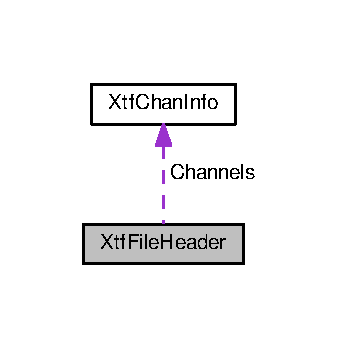
\includegraphics[width=164pt]{structXtfFileHeader__coll__graph}
\end{center}
\end{figure}
\subsection*{Attributs publics}
\begin{DoxyCompactItemize}
\item 
uint8\+\_\+t \hyperlink{structXtfFileHeader_a4316f8ddfc7a8aedc2ab48c57985cead}{File\+Format}
\item 
uint8\+\_\+t \hyperlink{structXtfFileHeader_a6f3eec78f338aa8f78a914d5e11eb954}{System\+Type}
\item 
char \hyperlink{structXtfFileHeader_a6c80b9e5aad45b5d9fa6473fd032ac18}{Recording\+Program\+Name} \mbox{[}8\mbox{]}
\item 
char \hyperlink{structXtfFileHeader_a5082997e4ac14d21f4a23bb33b1586a6}{Recording\+Program\+Version} \mbox{[}8\mbox{]}
\item 
char \hyperlink{structXtfFileHeader_ac6fbf63597b953a9bb4550cb6328714b}{Sonar\+Name} \mbox{[}16\mbox{]}
\item 
uint16\+\_\+t \hyperlink{structXtfFileHeader_a5fab4bc57578ce290587de30618a44be}{Sonar\+Type}
\item 
char \hyperlink{structXtfFileHeader_aa28fc6fe135e8f48ccb029d5af2e69a2}{Note\+String} \mbox{[}64\mbox{]}
\item 
char \hyperlink{structXtfFileHeader_ad14ce2faf476f95467619c8c6f67950d}{This\+File\+Name} \mbox{[}64\mbox{]}
\item 
uint16\+\_\+t \hyperlink{structXtfFileHeader_aa39461695c29091c125e9044ee6d89e8}{Nav\+Units}
\item 
uint16\+\_\+t \hyperlink{structXtfFileHeader_ab6f5f727287c8a02037cce63c5460ee1}{Number\+Of\+Sonar\+Channels}
\item 
uint16\+\_\+t \hyperlink{structXtfFileHeader_afea2149b1bf036eeed83ad103ec113a6}{Number\+Of\+Bathymetry\+Channels}
\item 
uint8\+\_\+t \hyperlink{structXtfFileHeader_a646498f4f1a07044827eee631b0c2643}{Number\+Of\+Snippet\+Channels}
\item 
uint8\+\_\+t \hyperlink{structXtfFileHeader_aeabf307d9c414577ace662cdadf3a0c3}{Number\+Of\+Forward\+Look\+Arrays}
\item 
uint16\+\_\+t \hyperlink{structXtfFileHeader_a603e8d0b78f105511178e866215c810a}{Number\+Of\+Echo\+Strength\+Channels}
\item 
uint8\+\_\+t \hyperlink{structXtfFileHeader_aca1155f0ad5bef9dadeadea7a39e2fd3}{Number\+Of\+Interferometry\+Channels}
\item 
uint8\+\_\+t \hyperlink{structXtfFileHeader_a7f71f2c11c7e7272f220495e8a622392}{Reserved1}
\item 
uint16\+\_\+t \hyperlink{structXtfFileHeader_ace47ee611ec4a68588f721b1b26e5e63}{Reserved2}
\item 
float \hyperlink{structXtfFileHeader_a6dbc0fdd85b3ced392a65effe583db3c}{Reference\+Point\+Height}
\item 
int8\+\_\+t \hyperlink{structXtfFileHeader_a08292e23bcee9ccbd738b098b288a919}{Projection\+Type} \mbox{[}12\mbox{]}
\item 
int8\+\_\+t \hyperlink{structXtfFileHeader_a634012d11a96a64b7844c105b44217bd}{Spheriod\+Type} \mbox{[}10\mbox{]}
\item 
int32\+\_\+t \hyperlink{structXtfFileHeader_a95cdc67cec15641bda7bc0addff5d414}{Navigation\+Latency}
\item 
float \hyperlink{structXtfFileHeader_a7b21704f379ce25117d694702045189c}{OriginY}
\item 
float \hyperlink{structXtfFileHeader_ab6e7da58bba25e17870f4666b5e07295}{OriginX}
\item 
float \hyperlink{structXtfFileHeader_a0d0cfe9d842a9445410d9f886b949927}{Nav\+OffsetY}
\item 
float \hyperlink{structXtfFileHeader_a49b9918649649708dae07261ea8f5a45}{Nav\+OffsetX}
\item 
float \hyperlink{structXtfFileHeader_aefb0b8f6ce50f860ede9943514738625}{Nav\+OffsetZ}
\item 
float \hyperlink{structXtfFileHeader_a22edd45c713124b52942185cfb4fa175}{Nav\+Offset\+Yaw}
\item 
float \hyperlink{structXtfFileHeader_ab3a315b69d166ce5e04d7e400cd0aed1}{M\+R\+U\+OffsetY}
\item 
float \hyperlink{structXtfFileHeader_aa5b7faae3076acae008aff436374d6e1}{M\+R\+U\+OffsetX}
\item 
float \hyperlink{structXtfFileHeader_a3094ed9e03b37b0924f46feae06f3c33}{M\+R\+U\+OffsetZ}
\item 
float \hyperlink{structXtfFileHeader_a70e48d6a8d5f2b869039e6a0a8839374}{M\+R\+U\+Offset\+Yaw}
\item 
float \hyperlink{structXtfFileHeader_aaadb5b9e13ee540523ad9806b75ca2ac}{M\+R\+U\+Offset\+Pitch}
\item 
float \hyperlink{structXtfFileHeader_a50244f5a0b3f6c96008a4de47c8c5ad1}{M\+R\+U\+Offset\+Roll}
\item 
\hyperlink{structXtfChanInfo}{Xtf\+Chan\+Info} \hyperlink{structXtfFileHeader_ab8e7fea8570e605686c319d86d99f1bc}{Channels} \mbox{[}6\mbox{]}
\end{DoxyCompactItemize}


\subsection{Documentation des données membres}
\mbox{\Hypertarget{structXtfFileHeader_ab8e7fea8570e605686c319d86d99f1bc}\label{structXtfFileHeader_ab8e7fea8570e605686c319d86d99f1bc}} 
\index{Xtf\+File\+Header@{Xtf\+File\+Header}!Channels@{Channels}}
\index{Channels@{Channels}!Xtf\+File\+Header@{Xtf\+File\+Header}}
\subsubsection{\texorpdfstring{Channels}{Channels}}
{\footnotesize\ttfamily \hyperlink{structXtfChanInfo}{Xtf\+Chan\+Info} Xtf\+File\+Header\+::\+Channels\mbox{[}6\mbox{]}}

\mbox{\Hypertarget{structXtfFileHeader_a4316f8ddfc7a8aedc2ab48c57985cead}\label{structXtfFileHeader_a4316f8ddfc7a8aedc2ab48c57985cead}} 
\index{Xtf\+File\+Header@{Xtf\+File\+Header}!File\+Format@{File\+Format}}
\index{File\+Format@{File\+Format}!Xtf\+File\+Header@{Xtf\+File\+Header}}
\subsubsection{\texorpdfstring{File\+Format}{FileFormat}}
{\footnotesize\ttfamily uint8\+\_\+t Xtf\+File\+Header\+::\+File\+Format}

\mbox{\Hypertarget{structXtfFileHeader_aaadb5b9e13ee540523ad9806b75ca2ac}\label{structXtfFileHeader_aaadb5b9e13ee540523ad9806b75ca2ac}} 
\index{Xtf\+File\+Header@{Xtf\+File\+Header}!M\+R\+U\+Offset\+Pitch@{M\+R\+U\+Offset\+Pitch}}
\index{M\+R\+U\+Offset\+Pitch@{M\+R\+U\+Offset\+Pitch}!Xtf\+File\+Header@{Xtf\+File\+Header}}
\subsubsection{\texorpdfstring{M\+R\+U\+Offset\+Pitch}{MRUOffsetPitch}}
{\footnotesize\ttfamily float Xtf\+File\+Header\+::\+M\+R\+U\+Offset\+Pitch}

\mbox{\Hypertarget{structXtfFileHeader_a50244f5a0b3f6c96008a4de47c8c5ad1}\label{structXtfFileHeader_a50244f5a0b3f6c96008a4de47c8c5ad1}} 
\index{Xtf\+File\+Header@{Xtf\+File\+Header}!M\+R\+U\+Offset\+Roll@{M\+R\+U\+Offset\+Roll}}
\index{M\+R\+U\+Offset\+Roll@{M\+R\+U\+Offset\+Roll}!Xtf\+File\+Header@{Xtf\+File\+Header}}
\subsubsection{\texorpdfstring{M\+R\+U\+Offset\+Roll}{MRUOffsetRoll}}
{\footnotesize\ttfamily float Xtf\+File\+Header\+::\+M\+R\+U\+Offset\+Roll}

\mbox{\Hypertarget{structXtfFileHeader_aa5b7faae3076acae008aff436374d6e1}\label{structXtfFileHeader_aa5b7faae3076acae008aff436374d6e1}} 
\index{Xtf\+File\+Header@{Xtf\+File\+Header}!M\+R\+U\+OffsetX@{M\+R\+U\+OffsetX}}
\index{M\+R\+U\+OffsetX@{M\+R\+U\+OffsetX}!Xtf\+File\+Header@{Xtf\+File\+Header}}
\subsubsection{\texorpdfstring{M\+R\+U\+OffsetX}{MRUOffsetX}}
{\footnotesize\ttfamily float Xtf\+File\+Header\+::\+M\+R\+U\+OffsetX}

\mbox{\Hypertarget{structXtfFileHeader_ab3a315b69d166ce5e04d7e400cd0aed1}\label{structXtfFileHeader_ab3a315b69d166ce5e04d7e400cd0aed1}} 
\index{Xtf\+File\+Header@{Xtf\+File\+Header}!M\+R\+U\+OffsetY@{M\+R\+U\+OffsetY}}
\index{M\+R\+U\+OffsetY@{M\+R\+U\+OffsetY}!Xtf\+File\+Header@{Xtf\+File\+Header}}
\subsubsection{\texorpdfstring{M\+R\+U\+OffsetY}{MRUOffsetY}}
{\footnotesize\ttfamily float Xtf\+File\+Header\+::\+M\+R\+U\+OffsetY}

\mbox{\Hypertarget{structXtfFileHeader_a70e48d6a8d5f2b869039e6a0a8839374}\label{structXtfFileHeader_a70e48d6a8d5f2b869039e6a0a8839374}} 
\index{Xtf\+File\+Header@{Xtf\+File\+Header}!M\+R\+U\+Offset\+Yaw@{M\+R\+U\+Offset\+Yaw}}
\index{M\+R\+U\+Offset\+Yaw@{M\+R\+U\+Offset\+Yaw}!Xtf\+File\+Header@{Xtf\+File\+Header}}
\subsubsection{\texorpdfstring{M\+R\+U\+Offset\+Yaw}{MRUOffsetYaw}}
{\footnotesize\ttfamily float Xtf\+File\+Header\+::\+M\+R\+U\+Offset\+Yaw}

\mbox{\Hypertarget{structXtfFileHeader_a3094ed9e03b37b0924f46feae06f3c33}\label{structXtfFileHeader_a3094ed9e03b37b0924f46feae06f3c33}} 
\index{Xtf\+File\+Header@{Xtf\+File\+Header}!M\+R\+U\+OffsetZ@{M\+R\+U\+OffsetZ}}
\index{M\+R\+U\+OffsetZ@{M\+R\+U\+OffsetZ}!Xtf\+File\+Header@{Xtf\+File\+Header}}
\subsubsection{\texorpdfstring{M\+R\+U\+OffsetZ}{MRUOffsetZ}}
{\footnotesize\ttfamily float Xtf\+File\+Header\+::\+M\+R\+U\+OffsetZ}

\mbox{\Hypertarget{structXtfFileHeader_a95cdc67cec15641bda7bc0addff5d414}\label{structXtfFileHeader_a95cdc67cec15641bda7bc0addff5d414}} 
\index{Xtf\+File\+Header@{Xtf\+File\+Header}!Navigation\+Latency@{Navigation\+Latency}}
\index{Navigation\+Latency@{Navigation\+Latency}!Xtf\+File\+Header@{Xtf\+File\+Header}}
\subsubsection{\texorpdfstring{Navigation\+Latency}{NavigationLatency}}
{\footnotesize\ttfamily int32\+\_\+t Xtf\+File\+Header\+::\+Navigation\+Latency}

\mbox{\Hypertarget{structXtfFileHeader_a49b9918649649708dae07261ea8f5a45}\label{structXtfFileHeader_a49b9918649649708dae07261ea8f5a45}} 
\index{Xtf\+File\+Header@{Xtf\+File\+Header}!Nav\+OffsetX@{Nav\+OffsetX}}
\index{Nav\+OffsetX@{Nav\+OffsetX}!Xtf\+File\+Header@{Xtf\+File\+Header}}
\subsubsection{\texorpdfstring{Nav\+OffsetX}{NavOffsetX}}
{\footnotesize\ttfamily float Xtf\+File\+Header\+::\+Nav\+OffsetX}

\mbox{\Hypertarget{structXtfFileHeader_a0d0cfe9d842a9445410d9f886b949927}\label{structXtfFileHeader_a0d0cfe9d842a9445410d9f886b949927}} 
\index{Xtf\+File\+Header@{Xtf\+File\+Header}!Nav\+OffsetY@{Nav\+OffsetY}}
\index{Nav\+OffsetY@{Nav\+OffsetY}!Xtf\+File\+Header@{Xtf\+File\+Header}}
\subsubsection{\texorpdfstring{Nav\+OffsetY}{NavOffsetY}}
{\footnotesize\ttfamily float Xtf\+File\+Header\+::\+Nav\+OffsetY}

\mbox{\Hypertarget{structXtfFileHeader_a22edd45c713124b52942185cfb4fa175}\label{structXtfFileHeader_a22edd45c713124b52942185cfb4fa175}} 
\index{Xtf\+File\+Header@{Xtf\+File\+Header}!Nav\+Offset\+Yaw@{Nav\+Offset\+Yaw}}
\index{Nav\+Offset\+Yaw@{Nav\+Offset\+Yaw}!Xtf\+File\+Header@{Xtf\+File\+Header}}
\subsubsection{\texorpdfstring{Nav\+Offset\+Yaw}{NavOffsetYaw}}
{\footnotesize\ttfamily float Xtf\+File\+Header\+::\+Nav\+Offset\+Yaw}

\mbox{\Hypertarget{structXtfFileHeader_aefb0b8f6ce50f860ede9943514738625}\label{structXtfFileHeader_aefb0b8f6ce50f860ede9943514738625}} 
\index{Xtf\+File\+Header@{Xtf\+File\+Header}!Nav\+OffsetZ@{Nav\+OffsetZ}}
\index{Nav\+OffsetZ@{Nav\+OffsetZ}!Xtf\+File\+Header@{Xtf\+File\+Header}}
\subsubsection{\texorpdfstring{Nav\+OffsetZ}{NavOffsetZ}}
{\footnotesize\ttfamily float Xtf\+File\+Header\+::\+Nav\+OffsetZ}

\mbox{\Hypertarget{structXtfFileHeader_aa39461695c29091c125e9044ee6d89e8}\label{structXtfFileHeader_aa39461695c29091c125e9044ee6d89e8}} 
\index{Xtf\+File\+Header@{Xtf\+File\+Header}!Nav\+Units@{Nav\+Units}}
\index{Nav\+Units@{Nav\+Units}!Xtf\+File\+Header@{Xtf\+File\+Header}}
\subsubsection{\texorpdfstring{Nav\+Units}{NavUnits}}
{\footnotesize\ttfamily uint16\+\_\+t Xtf\+File\+Header\+::\+Nav\+Units}

\mbox{\Hypertarget{structXtfFileHeader_aa28fc6fe135e8f48ccb029d5af2e69a2}\label{structXtfFileHeader_aa28fc6fe135e8f48ccb029d5af2e69a2}} 
\index{Xtf\+File\+Header@{Xtf\+File\+Header}!Note\+String@{Note\+String}}
\index{Note\+String@{Note\+String}!Xtf\+File\+Header@{Xtf\+File\+Header}}
\subsubsection{\texorpdfstring{Note\+String}{NoteString}}
{\footnotesize\ttfamily char Xtf\+File\+Header\+::\+Note\+String\mbox{[}64\mbox{]}}

\mbox{\Hypertarget{structXtfFileHeader_afea2149b1bf036eeed83ad103ec113a6}\label{structXtfFileHeader_afea2149b1bf036eeed83ad103ec113a6}} 
\index{Xtf\+File\+Header@{Xtf\+File\+Header}!Number\+Of\+Bathymetry\+Channels@{Number\+Of\+Bathymetry\+Channels}}
\index{Number\+Of\+Bathymetry\+Channels@{Number\+Of\+Bathymetry\+Channels}!Xtf\+File\+Header@{Xtf\+File\+Header}}
\subsubsection{\texorpdfstring{Number\+Of\+Bathymetry\+Channels}{NumberOfBathymetryChannels}}
{\footnotesize\ttfamily uint16\+\_\+t Xtf\+File\+Header\+::\+Number\+Of\+Bathymetry\+Channels}

\mbox{\Hypertarget{structXtfFileHeader_a603e8d0b78f105511178e866215c810a}\label{structXtfFileHeader_a603e8d0b78f105511178e866215c810a}} 
\index{Xtf\+File\+Header@{Xtf\+File\+Header}!Number\+Of\+Echo\+Strength\+Channels@{Number\+Of\+Echo\+Strength\+Channels}}
\index{Number\+Of\+Echo\+Strength\+Channels@{Number\+Of\+Echo\+Strength\+Channels}!Xtf\+File\+Header@{Xtf\+File\+Header}}
\subsubsection{\texorpdfstring{Number\+Of\+Echo\+Strength\+Channels}{NumberOfEchoStrengthChannels}}
{\footnotesize\ttfamily uint16\+\_\+t Xtf\+File\+Header\+::\+Number\+Of\+Echo\+Strength\+Channels}

\mbox{\Hypertarget{structXtfFileHeader_aeabf307d9c414577ace662cdadf3a0c3}\label{structXtfFileHeader_aeabf307d9c414577ace662cdadf3a0c3}} 
\index{Xtf\+File\+Header@{Xtf\+File\+Header}!Number\+Of\+Forward\+Look\+Arrays@{Number\+Of\+Forward\+Look\+Arrays}}
\index{Number\+Of\+Forward\+Look\+Arrays@{Number\+Of\+Forward\+Look\+Arrays}!Xtf\+File\+Header@{Xtf\+File\+Header}}
\subsubsection{\texorpdfstring{Number\+Of\+Forward\+Look\+Arrays}{NumberOfForwardLookArrays}}
{\footnotesize\ttfamily uint8\+\_\+t Xtf\+File\+Header\+::\+Number\+Of\+Forward\+Look\+Arrays}

\mbox{\Hypertarget{structXtfFileHeader_aca1155f0ad5bef9dadeadea7a39e2fd3}\label{structXtfFileHeader_aca1155f0ad5bef9dadeadea7a39e2fd3}} 
\index{Xtf\+File\+Header@{Xtf\+File\+Header}!Number\+Of\+Interferometry\+Channels@{Number\+Of\+Interferometry\+Channels}}
\index{Number\+Of\+Interferometry\+Channels@{Number\+Of\+Interferometry\+Channels}!Xtf\+File\+Header@{Xtf\+File\+Header}}
\subsubsection{\texorpdfstring{Number\+Of\+Interferometry\+Channels}{NumberOfInterferometryChannels}}
{\footnotesize\ttfamily uint8\+\_\+t Xtf\+File\+Header\+::\+Number\+Of\+Interferometry\+Channels}

\mbox{\Hypertarget{structXtfFileHeader_a646498f4f1a07044827eee631b0c2643}\label{structXtfFileHeader_a646498f4f1a07044827eee631b0c2643}} 
\index{Xtf\+File\+Header@{Xtf\+File\+Header}!Number\+Of\+Snippet\+Channels@{Number\+Of\+Snippet\+Channels}}
\index{Number\+Of\+Snippet\+Channels@{Number\+Of\+Snippet\+Channels}!Xtf\+File\+Header@{Xtf\+File\+Header}}
\subsubsection{\texorpdfstring{Number\+Of\+Snippet\+Channels}{NumberOfSnippetChannels}}
{\footnotesize\ttfamily uint8\+\_\+t Xtf\+File\+Header\+::\+Number\+Of\+Snippet\+Channels}

\mbox{\Hypertarget{structXtfFileHeader_ab6f5f727287c8a02037cce63c5460ee1}\label{structXtfFileHeader_ab6f5f727287c8a02037cce63c5460ee1}} 
\index{Xtf\+File\+Header@{Xtf\+File\+Header}!Number\+Of\+Sonar\+Channels@{Number\+Of\+Sonar\+Channels}}
\index{Number\+Of\+Sonar\+Channels@{Number\+Of\+Sonar\+Channels}!Xtf\+File\+Header@{Xtf\+File\+Header}}
\subsubsection{\texorpdfstring{Number\+Of\+Sonar\+Channels}{NumberOfSonarChannels}}
{\footnotesize\ttfamily uint16\+\_\+t Xtf\+File\+Header\+::\+Number\+Of\+Sonar\+Channels}

\mbox{\Hypertarget{structXtfFileHeader_ab6e7da58bba25e17870f4666b5e07295}\label{structXtfFileHeader_ab6e7da58bba25e17870f4666b5e07295}} 
\index{Xtf\+File\+Header@{Xtf\+File\+Header}!OriginX@{OriginX}}
\index{OriginX@{OriginX}!Xtf\+File\+Header@{Xtf\+File\+Header}}
\subsubsection{\texorpdfstring{OriginX}{OriginX}}
{\footnotesize\ttfamily float Xtf\+File\+Header\+::\+OriginX}

\mbox{\Hypertarget{structXtfFileHeader_a7b21704f379ce25117d694702045189c}\label{structXtfFileHeader_a7b21704f379ce25117d694702045189c}} 
\index{Xtf\+File\+Header@{Xtf\+File\+Header}!OriginY@{OriginY}}
\index{OriginY@{OriginY}!Xtf\+File\+Header@{Xtf\+File\+Header}}
\subsubsection{\texorpdfstring{OriginY}{OriginY}}
{\footnotesize\ttfamily float Xtf\+File\+Header\+::\+OriginY}

\mbox{\Hypertarget{structXtfFileHeader_a08292e23bcee9ccbd738b098b288a919}\label{structXtfFileHeader_a08292e23bcee9ccbd738b098b288a919}} 
\index{Xtf\+File\+Header@{Xtf\+File\+Header}!Projection\+Type@{Projection\+Type}}
\index{Projection\+Type@{Projection\+Type}!Xtf\+File\+Header@{Xtf\+File\+Header}}
\subsubsection{\texorpdfstring{Projection\+Type}{ProjectionType}}
{\footnotesize\ttfamily int8\+\_\+t Xtf\+File\+Header\+::\+Projection\+Type\mbox{[}12\mbox{]}}

\mbox{\Hypertarget{structXtfFileHeader_a6c80b9e5aad45b5d9fa6473fd032ac18}\label{structXtfFileHeader_a6c80b9e5aad45b5d9fa6473fd032ac18}} 
\index{Xtf\+File\+Header@{Xtf\+File\+Header}!Recording\+Program\+Name@{Recording\+Program\+Name}}
\index{Recording\+Program\+Name@{Recording\+Program\+Name}!Xtf\+File\+Header@{Xtf\+File\+Header}}
\subsubsection{\texorpdfstring{Recording\+Program\+Name}{RecordingProgramName}}
{\footnotesize\ttfamily char Xtf\+File\+Header\+::\+Recording\+Program\+Name\mbox{[}8\mbox{]}}

\mbox{\Hypertarget{structXtfFileHeader_a5082997e4ac14d21f4a23bb33b1586a6}\label{structXtfFileHeader_a5082997e4ac14d21f4a23bb33b1586a6}} 
\index{Xtf\+File\+Header@{Xtf\+File\+Header}!Recording\+Program\+Version@{Recording\+Program\+Version}}
\index{Recording\+Program\+Version@{Recording\+Program\+Version}!Xtf\+File\+Header@{Xtf\+File\+Header}}
\subsubsection{\texorpdfstring{Recording\+Program\+Version}{RecordingProgramVersion}}
{\footnotesize\ttfamily char Xtf\+File\+Header\+::\+Recording\+Program\+Version\mbox{[}8\mbox{]}}

\mbox{\Hypertarget{structXtfFileHeader_a6dbc0fdd85b3ced392a65effe583db3c}\label{structXtfFileHeader_a6dbc0fdd85b3ced392a65effe583db3c}} 
\index{Xtf\+File\+Header@{Xtf\+File\+Header}!Reference\+Point\+Height@{Reference\+Point\+Height}}
\index{Reference\+Point\+Height@{Reference\+Point\+Height}!Xtf\+File\+Header@{Xtf\+File\+Header}}
\subsubsection{\texorpdfstring{Reference\+Point\+Height}{ReferencePointHeight}}
{\footnotesize\ttfamily float Xtf\+File\+Header\+::\+Reference\+Point\+Height}

\mbox{\Hypertarget{structXtfFileHeader_a7f71f2c11c7e7272f220495e8a622392}\label{structXtfFileHeader_a7f71f2c11c7e7272f220495e8a622392}} 
\index{Xtf\+File\+Header@{Xtf\+File\+Header}!Reserved1@{Reserved1}}
\index{Reserved1@{Reserved1}!Xtf\+File\+Header@{Xtf\+File\+Header}}
\subsubsection{\texorpdfstring{Reserved1}{Reserved1}}
{\footnotesize\ttfamily uint8\+\_\+t Xtf\+File\+Header\+::\+Reserved1}

\mbox{\Hypertarget{structXtfFileHeader_ace47ee611ec4a68588f721b1b26e5e63}\label{structXtfFileHeader_ace47ee611ec4a68588f721b1b26e5e63}} 
\index{Xtf\+File\+Header@{Xtf\+File\+Header}!Reserved2@{Reserved2}}
\index{Reserved2@{Reserved2}!Xtf\+File\+Header@{Xtf\+File\+Header}}
\subsubsection{\texorpdfstring{Reserved2}{Reserved2}}
{\footnotesize\ttfamily uint16\+\_\+t Xtf\+File\+Header\+::\+Reserved2}

\mbox{\Hypertarget{structXtfFileHeader_ac6fbf63597b953a9bb4550cb6328714b}\label{structXtfFileHeader_ac6fbf63597b953a9bb4550cb6328714b}} 
\index{Xtf\+File\+Header@{Xtf\+File\+Header}!Sonar\+Name@{Sonar\+Name}}
\index{Sonar\+Name@{Sonar\+Name}!Xtf\+File\+Header@{Xtf\+File\+Header}}
\subsubsection{\texorpdfstring{Sonar\+Name}{SonarName}}
{\footnotesize\ttfamily char Xtf\+File\+Header\+::\+Sonar\+Name\mbox{[}16\mbox{]}}

\mbox{\Hypertarget{structXtfFileHeader_a5fab4bc57578ce290587de30618a44be}\label{structXtfFileHeader_a5fab4bc57578ce290587de30618a44be}} 
\index{Xtf\+File\+Header@{Xtf\+File\+Header}!Sonar\+Type@{Sonar\+Type}}
\index{Sonar\+Type@{Sonar\+Type}!Xtf\+File\+Header@{Xtf\+File\+Header}}
\subsubsection{\texorpdfstring{Sonar\+Type}{SonarType}}
{\footnotesize\ttfamily uint16\+\_\+t Xtf\+File\+Header\+::\+Sonar\+Type}

\mbox{\Hypertarget{structXtfFileHeader_a634012d11a96a64b7844c105b44217bd}\label{structXtfFileHeader_a634012d11a96a64b7844c105b44217bd}} 
\index{Xtf\+File\+Header@{Xtf\+File\+Header}!Spheriod\+Type@{Spheriod\+Type}}
\index{Spheriod\+Type@{Spheriod\+Type}!Xtf\+File\+Header@{Xtf\+File\+Header}}
\subsubsection{\texorpdfstring{Spheriod\+Type}{SpheriodType}}
{\footnotesize\ttfamily int8\+\_\+t Xtf\+File\+Header\+::\+Spheriod\+Type\mbox{[}10\mbox{]}}

\mbox{\Hypertarget{structXtfFileHeader_a6f3eec78f338aa8f78a914d5e11eb954}\label{structXtfFileHeader_a6f3eec78f338aa8f78a914d5e11eb954}} 
\index{Xtf\+File\+Header@{Xtf\+File\+Header}!System\+Type@{System\+Type}}
\index{System\+Type@{System\+Type}!Xtf\+File\+Header@{Xtf\+File\+Header}}
\subsubsection{\texorpdfstring{System\+Type}{SystemType}}
{\footnotesize\ttfamily uint8\+\_\+t Xtf\+File\+Header\+::\+System\+Type}

\mbox{\Hypertarget{structXtfFileHeader_ad14ce2faf476f95467619c8c6f67950d}\label{structXtfFileHeader_ad14ce2faf476f95467619c8c6f67950d}} 
\index{Xtf\+File\+Header@{Xtf\+File\+Header}!This\+File\+Name@{This\+File\+Name}}
\index{This\+File\+Name@{This\+File\+Name}!Xtf\+File\+Header@{Xtf\+File\+Header}}
\subsubsection{\texorpdfstring{This\+File\+Name}{ThisFileName}}
{\footnotesize\ttfamily char Xtf\+File\+Header\+::\+This\+File\+Name\mbox{[}64\mbox{]}}



La documentation de cette structure a été générée à partir du fichier suivant \+:\begin{DoxyCompactItemize}
\item 
src/datagrams/xtf/\hyperlink{XtfTypes_8hpp}{Xtf\+Types.\+hpp}\end{DoxyCompactItemize}

\hypertarget{structXtfHeaderGyro}{}\section{Référence de la structure Xtf\+Header\+Gyro}
\label{structXtfHeaderGyro}\index{Xtf\+Header\+Gyro@{Xtf\+Header\+Gyro}}


{\ttfamily \#include $<$Xtf\+Types.\+hpp$>$}

\subsection*{Attributs publics}
\begin{DoxyCompactItemize}
\item 
uint16\+\_\+t \hyperlink{structXtfHeaderGyro_a0c3ec12cdab19969fef3b141a98ec362}{Magic\+Number}
\item 
uint8\+\_\+t \hyperlink{structXtfHeaderGyro_ab28e7efcda9242b4bdb08557b16beb90}{Header\+Type}
\item 
uint8\+\_\+t \hyperlink{structXtfHeaderGyro_a85940ad89d69a78b55a3428577a3b21c}{Reserved} \mbox{[}7\mbox{]}
\item 
uint32\+\_\+t \hyperlink{structXtfHeaderGyro_a25420e37b193405adaed1b85ee7dc333}{Num\+Bytes\+This\+Record}
\item 
uint16\+\_\+t \hyperlink{structXtfHeaderGyro_aec617ad1ae79153ed3ad307d5aec9227}{Year}
\item 
uint8\+\_\+t \hyperlink{structXtfHeaderGyro_a7822067786a415fc90162384d72efff3}{Month}
\item 
uint8\+\_\+t \hyperlink{structXtfHeaderGyro_ad963020beeee806b7c5b8f82d9dd5715}{Day}
\item 
uint8\+\_\+t \hyperlink{structXtfHeaderGyro_a85f39f92d2f7ebb061b4cf601d8d9bfe}{Hour}
\item 
uint8\+\_\+t \hyperlink{structXtfHeaderGyro_a45f17b015a2311abbee3b6d22394c847}{Minute}
\item 
uint8\+\_\+t \hyperlink{structXtfHeaderGyro_ad741b6ad2d21952b9a5e202a2094790f}{Second}
\item 
uint32\+\_\+t \hyperlink{structXtfHeaderGyro_a1f17dc26ed56dd39571ab7659d728ac0}{Microseconds}
\item 
uint32\+\_\+t \hyperlink{structXtfHeaderGyro_a9ff2dd72393e49ab1fce01c1aae9e8c1}{Source\+Epoch}
\item 
uint32\+\_\+t \hyperlink{structXtfHeaderGyro_acca62eccaf3ac7899aac8414d8063b95}{Time\+Tag}
\item 
float \hyperlink{structXtfHeaderGyro_a069ec7f3085ca15e4e22e6d499c28244}{Gyro}
\item 
uint8\+\_\+t \hyperlink{structXtfHeaderGyro_af5a9a099f4f8950c1d77aeac02540dd7}{Time\+Flag}
\item 
uint8\+\_\+t \hyperlink{structXtfHeaderGyro_a567afc36a3461856d6563cd4249d68c0}{Reserved1} \mbox{[}26\mbox{]}
\end{DoxyCompactItemize}


\subsection{Documentation des données membres}
\mbox{\Hypertarget{structXtfHeaderGyro_ad963020beeee806b7c5b8f82d9dd5715}\label{structXtfHeaderGyro_ad963020beeee806b7c5b8f82d9dd5715}} 
\index{Xtf\+Header\+Gyro@{Xtf\+Header\+Gyro}!Day@{Day}}
\index{Day@{Day}!Xtf\+Header\+Gyro@{Xtf\+Header\+Gyro}}
\subsubsection{\texorpdfstring{Day}{Day}}
{\footnotesize\ttfamily uint8\+\_\+t Xtf\+Header\+Gyro\+::\+Day}

\mbox{\Hypertarget{structXtfHeaderGyro_a069ec7f3085ca15e4e22e6d499c28244}\label{structXtfHeaderGyro_a069ec7f3085ca15e4e22e6d499c28244}} 
\index{Xtf\+Header\+Gyro@{Xtf\+Header\+Gyro}!Gyro@{Gyro}}
\index{Gyro@{Gyro}!Xtf\+Header\+Gyro@{Xtf\+Header\+Gyro}}
\subsubsection{\texorpdfstring{Gyro}{Gyro}}
{\footnotesize\ttfamily float Xtf\+Header\+Gyro\+::\+Gyro}

\mbox{\Hypertarget{structXtfHeaderGyro_ab28e7efcda9242b4bdb08557b16beb90}\label{structXtfHeaderGyro_ab28e7efcda9242b4bdb08557b16beb90}} 
\index{Xtf\+Header\+Gyro@{Xtf\+Header\+Gyro}!Header\+Type@{Header\+Type}}
\index{Header\+Type@{Header\+Type}!Xtf\+Header\+Gyro@{Xtf\+Header\+Gyro}}
\subsubsection{\texorpdfstring{Header\+Type}{HeaderType}}
{\footnotesize\ttfamily uint8\+\_\+t Xtf\+Header\+Gyro\+::\+Header\+Type}

\mbox{\Hypertarget{structXtfHeaderGyro_a85f39f92d2f7ebb061b4cf601d8d9bfe}\label{structXtfHeaderGyro_a85f39f92d2f7ebb061b4cf601d8d9bfe}} 
\index{Xtf\+Header\+Gyro@{Xtf\+Header\+Gyro}!Hour@{Hour}}
\index{Hour@{Hour}!Xtf\+Header\+Gyro@{Xtf\+Header\+Gyro}}
\subsubsection{\texorpdfstring{Hour}{Hour}}
{\footnotesize\ttfamily uint8\+\_\+t Xtf\+Header\+Gyro\+::\+Hour}

\mbox{\Hypertarget{structXtfHeaderGyro_a0c3ec12cdab19969fef3b141a98ec362}\label{structXtfHeaderGyro_a0c3ec12cdab19969fef3b141a98ec362}} 
\index{Xtf\+Header\+Gyro@{Xtf\+Header\+Gyro}!Magic\+Number@{Magic\+Number}}
\index{Magic\+Number@{Magic\+Number}!Xtf\+Header\+Gyro@{Xtf\+Header\+Gyro}}
\subsubsection{\texorpdfstring{Magic\+Number}{MagicNumber}}
{\footnotesize\ttfamily uint16\+\_\+t Xtf\+Header\+Gyro\+::\+Magic\+Number}

\mbox{\Hypertarget{structXtfHeaderGyro_a1f17dc26ed56dd39571ab7659d728ac0}\label{structXtfHeaderGyro_a1f17dc26ed56dd39571ab7659d728ac0}} 
\index{Xtf\+Header\+Gyro@{Xtf\+Header\+Gyro}!Microseconds@{Microseconds}}
\index{Microseconds@{Microseconds}!Xtf\+Header\+Gyro@{Xtf\+Header\+Gyro}}
\subsubsection{\texorpdfstring{Microseconds}{Microseconds}}
{\footnotesize\ttfamily uint32\+\_\+t Xtf\+Header\+Gyro\+::\+Microseconds}

\mbox{\Hypertarget{structXtfHeaderGyro_a45f17b015a2311abbee3b6d22394c847}\label{structXtfHeaderGyro_a45f17b015a2311abbee3b6d22394c847}} 
\index{Xtf\+Header\+Gyro@{Xtf\+Header\+Gyro}!Minute@{Minute}}
\index{Minute@{Minute}!Xtf\+Header\+Gyro@{Xtf\+Header\+Gyro}}
\subsubsection{\texorpdfstring{Minute}{Minute}}
{\footnotesize\ttfamily uint8\+\_\+t Xtf\+Header\+Gyro\+::\+Minute}

\mbox{\Hypertarget{structXtfHeaderGyro_a7822067786a415fc90162384d72efff3}\label{structXtfHeaderGyro_a7822067786a415fc90162384d72efff3}} 
\index{Xtf\+Header\+Gyro@{Xtf\+Header\+Gyro}!Month@{Month}}
\index{Month@{Month}!Xtf\+Header\+Gyro@{Xtf\+Header\+Gyro}}
\subsubsection{\texorpdfstring{Month}{Month}}
{\footnotesize\ttfamily uint8\+\_\+t Xtf\+Header\+Gyro\+::\+Month}

\mbox{\Hypertarget{structXtfHeaderGyro_a25420e37b193405adaed1b85ee7dc333}\label{structXtfHeaderGyro_a25420e37b193405adaed1b85ee7dc333}} 
\index{Xtf\+Header\+Gyro@{Xtf\+Header\+Gyro}!Num\+Bytes\+This\+Record@{Num\+Bytes\+This\+Record}}
\index{Num\+Bytes\+This\+Record@{Num\+Bytes\+This\+Record}!Xtf\+Header\+Gyro@{Xtf\+Header\+Gyro}}
\subsubsection{\texorpdfstring{Num\+Bytes\+This\+Record}{NumBytesThisRecord}}
{\footnotesize\ttfamily uint32\+\_\+t Xtf\+Header\+Gyro\+::\+Num\+Bytes\+This\+Record}

\mbox{\Hypertarget{structXtfHeaderGyro_a85940ad89d69a78b55a3428577a3b21c}\label{structXtfHeaderGyro_a85940ad89d69a78b55a3428577a3b21c}} 
\index{Xtf\+Header\+Gyro@{Xtf\+Header\+Gyro}!Reserved@{Reserved}}
\index{Reserved@{Reserved}!Xtf\+Header\+Gyro@{Xtf\+Header\+Gyro}}
\subsubsection{\texorpdfstring{Reserved}{Reserved}}
{\footnotesize\ttfamily uint8\+\_\+t Xtf\+Header\+Gyro\+::\+Reserved\mbox{[}7\mbox{]}}

\mbox{\Hypertarget{structXtfHeaderGyro_a567afc36a3461856d6563cd4249d68c0}\label{structXtfHeaderGyro_a567afc36a3461856d6563cd4249d68c0}} 
\index{Xtf\+Header\+Gyro@{Xtf\+Header\+Gyro}!Reserved1@{Reserved1}}
\index{Reserved1@{Reserved1}!Xtf\+Header\+Gyro@{Xtf\+Header\+Gyro}}
\subsubsection{\texorpdfstring{Reserved1}{Reserved1}}
{\footnotesize\ttfamily uint8\+\_\+t Xtf\+Header\+Gyro\+::\+Reserved1\mbox{[}26\mbox{]}}

\mbox{\Hypertarget{structXtfHeaderGyro_ad741b6ad2d21952b9a5e202a2094790f}\label{structXtfHeaderGyro_ad741b6ad2d21952b9a5e202a2094790f}} 
\index{Xtf\+Header\+Gyro@{Xtf\+Header\+Gyro}!Second@{Second}}
\index{Second@{Second}!Xtf\+Header\+Gyro@{Xtf\+Header\+Gyro}}
\subsubsection{\texorpdfstring{Second}{Second}}
{\footnotesize\ttfamily uint8\+\_\+t Xtf\+Header\+Gyro\+::\+Second}

\mbox{\Hypertarget{structXtfHeaderGyro_a9ff2dd72393e49ab1fce01c1aae9e8c1}\label{structXtfHeaderGyro_a9ff2dd72393e49ab1fce01c1aae9e8c1}} 
\index{Xtf\+Header\+Gyro@{Xtf\+Header\+Gyro}!Source\+Epoch@{Source\+Epoch}}
\index{Source\+Epoch@{Source\+Epoch}!Xtf\+Header\+Gyro@{Xtf\+Header\+Gyro}}
\subsubsection{\texorpdfstring{Source\+Epoch}{SourceEpoch}}
{\footnotesize\ttfamily uint32\+\_\+t Xtf\+Header\+Gyro\+::\+Source\+Epoch}

\mbox{\Hypertarget{structXtfHeaderGyro_af5a9a099f4f8950c1d77aeac02540dd7}\label{structXtfHeaderGyro_af5a9a099f4f8950c1d77aeac02540dd7}} 
\index{Xtf\+Header\+Gyro@{Xtf\+Header\+Gyro}!Time\+Flag@{Time\+Flag}}
\index{Time\+Flag@{Time\+Flag}!Xtf\+Header\+Gyro@{Xtf\+Header\+Gyro}}
\subsubsection{\texorpdfstring{Time\+Flag}{TimeFlag}}
{\footnotesize\ttfamily uint8\+\_\+t Xtf\+Header\+Gyro\+::\+Time\+Flag}

\mbox{\Hypertarget{structXtfHeaderGyro_acca62eccaf3ac7899aac8414d8063b95}\label{structXtfHeaderGyro_acca62eccaf3ac7899aac8414d8063b95}} 
\index{Xtf\+Header\+Gyro@{Xtf\+Header\+Gyro}!Time\+Tag@{Time\+Tag}}
\index{Time\+Tag@{Time\+Tag}!Xtf\+Header\+Gyro@{Xtf\+Header\+Gyro}}
\subsubsection{\texorpdfstring{Time\+Tag}{TimeTag}}
{\footnotesize\ttfamily uint32\+\_\+t Xtf\+Header\+Gyro\+::\+Time\+Tag}

\mbox{\Hypertarget{structXtfHeaderGyro_aec617ad1ae79153ed3ad307d5aec9227}\label{structXtfHeaderGyro_aec617ad1ae79153ed3ad307d5aec9227}} 
\index{Xtf\+Header\+Gyro@{Xtf\+Header\+Gyro}!Year@{Year}}
\index{Year@{Year}!Xtf\+Header\+Gyro@{Xtf\+Header\+Gyro}}
\subsubsection{\texorpdfstring{Year}{Year}}
{\footnotesize\ttfamily uint16\+\_\+t Xtf\+Header\+Gyro\+::\+Year}



La documentation de cette structure a été générée à partir du fichier suivant \+:\begin{DoxyCompactItemize}
\item 
src/datagrams/xtf/\hyperlink{XtfTypes_8hpp}{Xtf\+Types.\+hpp}\end{DoxyCompactItemize}

\hypertarget{structXtfHeaderNavigation__type42}{}\section{Référence de la structure Xtf\+Header\+Navigation\+\_\+type42}
\label{structXtfHeaderNavigation__type42}\index{Xtf\+Header\+Navigation\+\_\+type42@{Xtf\+Header\+Navigation\+\_\+type42}}


{\ttfamily \#include $<$Xtf\+Types.\+hpp$>$}

\subsection*{Attributs publics}
\begin{DoxyCompactItemize}
\item 
uint16\+\_\+t \hyperlink{structXtfHeaderNavigation__type42_abd77970d2f172855cca6431c58d73cdf}{Magic\+Number}
\item 
uint8\+\_\+t \hyperlink{structXtfHeaderNavigation__type42_ae1d4cf5c81e5531928d5a21995ff2ef9}{Header\+Type}
\item 
uint8\+\_\+t \hyperlink{structXtfHeaderNavigation__type42_aa4b5d2746d6a3ca2b31befc7b3093d15}{Reserved} \mbox{[}7\mbox{]}
\item 
uint32\+\_\+t \hyperlink{structXtfHeaderNavigation__type42_a67c9b86f18b1b4d7b59e44949e86c1f0}{Num\+Bytes\+This\+Record}
\item 
uint16\+\_\+t \hyperlink{structXtfHeaderNavigation__type42_adc35d4b1ece422574a91829b3330a266}{Year}
\item 
uint8\+\_\+t \hyperlink{structXtfHeaderNavigation__type42_a385fba14ef74fe1f0487fa2bdb59ec9a}{Month}
\item 
uint8\+\_\+t \hyperlink{structXtfHeaderNavigation__type42_a7c70b71cc00baad0a1bc00ecb129c024}{Day}
\item 
uint8\+\_\+t \hyperlink{structXtfHeaderNavigation__type42_a6525083696ba2e06651009fbf05763e9}{Hour}
\item 
uint8\+\_\+t \hyperlink{structXtfHeaderNavigation__type42_a9277d358b25eefd262a8458de5a0b03d}{Minute}
\item 
uint8\+\_\+t \hyperlink{structXtfHeaderNavigation__type42_a82406f8d6f9c3ca70a7930a21a4c13a9}{Second}
\item 
uint32\+\_\+t \hyperlink{structXtfHeaderNavigation__type42_abaff8116ae9d1ae8219051b8b401daeb}{Microseconds}
\item 
uint32\+\_\+t \hyperlink{structXtfHeaderNavigation__type42_a546065eb5e81337ae20c3e5c8ca7d464}{Source\+Epoch}
\item 
uint32\+\_\+t \hyperlink{structXtfHeaderNavigation__type42_acfee8cdd16d7c8cf60b7ac45063201d2}{Time\+Tag}
\item 
double \hyperlink{structXtfHeaderNavigation__type42_af9a5d74604bb99d0038debce509d439b}{Raw\+Y\+Coordinate}
\item 
double \hyperlink{structXtfHeaderNavigation__type42_a6937fe7ddbe379b406a5dc8c0e0abff7}{Raw\+X\+Coordinate}
\item 
double \hyperlink{structXtfHeaderNavigation__type42_a983c6ce2d445facd41f9730460dea053}{Raw\+Altitude}
\item 
uint8\+\_\+t \hyperlink{structXtfHeaderNavigation__type42_a4c21a09dc13268493d80343352ebe9fe}{Time\+Flag}
\item 
uint8\+\_\+t \hyperlink{structXtfHeaderNavigation__type42_a1acbbea606cb7213d43633fd6459da27}{Reserved1} \mbox{[}6\mbox{]}
\end{DoxyCompactItemize}


\subsection{Documentation des données membres}
\mbox{\Hypertarget{structXtfHeaderNavigation__type42_a7c70b71cc00baad0a1bc00ecb129c024}\label{structXtfHeaderNavigation__type42_a7c70b71cc00baad0a1bc00ecb129c024}} 
\index{Xtf\+Header\+Navigation\+\_\+type42@{Xtf\+Header\+Navigation\+\_\+type42}!Day@{Day}}
\index{Day@{Day}!Xtf\+Header\+Navigation\+\_\+type42@{Xtf\+Header\+Navigation\+\_\+type42}}
\subsubsection{\texorpdfstring{Day}{Day}}
{\footnotesize\ttfamily uint8\+\_\+t Xtf\+Header\+Navigation\+\_\+type42\+::\+Day}

\mbox{\Hypertarget{structXtfHeaderNavigation__type42_ae1d4cf5c81e5531928d5a21995ff2ef9}\label{structXtfHeaderNavigation__type42_ae1d4cf5c81e5531928d5a21995ff2ef9}} 
\index{Xtf\+Header\+Navigation\+\_\+type42@{Xtf\+Header\+Navigation\+\_\+type42}!Header\+Type@{Header\+Type}}
\index{Header\+Type@{Header\+Type}!Xtf\+Header\+Navigation\+\_\+type42@{Xtf\+Header\+Navigation\+\_\+type42}}
\subsubsection{\texorpdfstring{Header\+Type}{HeaderType}}
{\footnotesize\ttfamily uint8\+\_\+t Xtf\+Header\+Navigation\+\_\+type42\+::\+Header\+Type}

\mbox{\Hypertarget{structXtfHeaderNavigation__type42_a6525083696ba2e06651009fbf05763e9}\label{structXtfHeaderNavigation__type42_a6525083696ba2e06651009fbf05763e9}} 
\index{Xtf\+Header\+Navigation\+\_\+type42@{Xtf\+Header\+Navigation\+\_\+type42}!Hour@{Hour}}
\index{Hour@{Hour}!Xtf\+Header\+Navigation\+\_\+type42@{Xtf\+Header\+Navigation\+\_\+type42}}
\subsubsection{\texorpdfstring{Hour}{Hour}}
{\footnotesize\ttfamily uint8\+\_\+t Xtf\+Header\+Navigation\+\_\+type42\+::\+Hour}

\mbox{\Hypertarget{structXtfHeaderNavigation__type42_abd77970d2f172855cca6431c58d73cdf}\label{structXtfHeaderNavigation__type42_abd77970d2f172855cca6431c58d73cdf}} 
\index{Xtf\+Header\+Navigation\+\_\+type42@{Xtf\+Header\+Navigation\+\_\+type42}!Magic\+Number@{Magic\+Number}}
\index{Magic\+Number@{Magic\+Number}!Xtf\+Header\+Navigation\+\_\+type42@{Xtf\+Header\+Navigation\+\_\+type42}}
\subsubsection{\texorpdfstring{Magic\+Number}{MagicNumber}}
{\footnotesize\ttfamily uint16\+\_\+t Xtf\+Header\+Navigation\+\_\+type42\+::\+Magic\+Number}

\mbox{\Hypertarget{structXtfHeaderNavigation__type42_abaff8116ae9d1ae8219051b8b401daeb}\label{structXtfHeaderNavigation__type42_abaff8116ae9d1ae8219051b8b401daeb}} 
\index{Xtf\+Header\+Navigation\+\_\+type42@{Xtf\+Header\+Navigation\+\_\+type42}!Microseconds@{Microseconds}}
\index{Microseconds@{Microseconds}!Xtf\+Header\+Navigation\+\_\+type42@{Xtf\+Header\+Navigation\+\_\+type42}}
\subsubsection{\texorpdfstring{Microseconds}{Microseconds}}
{\footnotesize\ttfamily uint32\+\_\+t Xtf\+Header\+Navigation\+\_\+type42\+::\+Microseconds}

\mbox{\Hypertarget{structXtfHeaderNavigation__type42_a9277d358b25eefd262a8458de5a0b03d}\label{structXtfHeaderNavigation__type42_a9277d358b25eefd262a8458de5a0b03d}} 
\index{Xtf\+Header\+Navigation\+\_\+type42@{Xtf\+Header\+Navigation\+\_\+type42}!Minute@{Minute}}
\index{Minute@{Minute}!Xtf\+Header\+Navigation\+\_\+type42@{Xtf\+Header\+Navigation\+\_\+type42}}
\subsubsection{\texorpdfstring{Minute}{Minute}}
{\footnotesize\ttfamily uint8\+\_\+t Xtf\+Header\+Navigation\+\_\+type42\+::\+Minute}

\mbox{\Hypertarget{structXtfHeaderNavigation__type42_a385fba14ef74fe1f0487fa2bdb59ec9a}\label{structXtfHeaderNavigation__type42_a385fba14ef74fe1f0487fa2bdb59ec9a}} 
\index{Xtf\+Header\+Navigation\+\_\+type42@{Xtf\+Header\+Navigation\+\_\+type42}!Month@{Month}}
\index{Month@{Month}!Xtf\+Header\+Navigation\+\_\+type42@{Xtf\+Header\+Navigation\+\_\+type42}}
\subsubsection{\texorpdfstring{Month}{Month}}
{\footnotesize\ttfamily uint8\+\_\+t Xtf\+Header\+Navigation\+\_\+type42\+::\+Month}

\mbox{\Hypertarget{structXtfHeaderNavigation__type42_a67c9b86f18b1b4d7b59e44949e86c1f0}\label{structXtfHeaderNavigation__type42_a67c9b86f18b1b4d7b59e44949e86c1f0}} 
\index{Xtf\+Header\+Navigation\+\_\+type42@{Xtf\+Header\+Navigation\+\_\+type42}!Num\+Bytes\+This\+Record@{Num\+Bytes\+This\+Record}}
\index{Num\+Bytes\+This\+Record@{Num\+Bytes\+This\+Record}!Xtf\+Header\+Navigation\+\_\+type42@{Xtf\+Header\+Navigation\+\_\+type42}}
\subsubsection{\texorpdfstring{Num\+Bytes\+This\+Record}{NumBytesThisRecord}}
{\footnotesize\ttfamily uint32\+\_\+t Xtf\+Header\+Navigation\+\_\+type42\+::\+Num\+Bytes\+This\+Record}

\mbox{\Hypertarget{structXtfHeaderNavigation__type42_a983c6ce2d445facd41f9730460dea053}\label{structXtfHeaderNavigation__type42_a983c6ce2d445facd41f9730460dea053}} 
\index{Xtf\+Header\+Navigation\+\_\+type42@{Xtf\+Header\+Navigation\+\_\+type42}!Raw\+Altitude@{Raw\+Altitude}}
\index{Raw\+Altitude@{Raw\+Altitude}!Xtf\+Header\+Navigation\+\_\+type42@{Xtf\+Header\+Navigation\+\_\+type42}}
\subsubsection{\texorpdfstring{Raw\+Altitude}{RawAltitude}}
{\footnotesize\ttfamily double Xtf\+Header\+Navigation\+\_\+type42\+::\+Raw\+Altitude}

\mbox{\Hypertarget{structXtfHeaderNavigation__type42_a6937fe7ddbe379b406a5dc8c0e0abff7}\label{structXtfHeaderNavigation__type42_a6937fe7ddbe379b406a5dc8c0e0abff7}} 
\index{Xtf\+Header\+Navigation\+\_\+type42@{Xtf\+Header\+Navigation\+\_\+type42}!Raw\+X\+Coordinate@{Raw\+X\+Coordinate}}
\index{Raw\+X\+Coordinate@{Raw\+X\+Coordinate}!Xtf\+Header\+Navigation\+\_\+type42@{Xtf\+Header\+Navigation\+\_\+type42}}
\subsubsection{\texorpdfstring{Raw\+X\+Coordinate}{RawXCoordinate}}
{\footnotesize\ttfamily double Xtf\+Header\+Navigation\+\_\+type42\+::\+Raw\+X\+Coordinate}

\mbox{\Hypertarget{structXtfHeaderNavigation__type42_af9a5d74604bb99d0038debce509d439b}\label{structXtfHeaderNavigation__type42_af9a5d74604bb99d0038debce509d439b}} 
\index{Xtf\+Header\+Navigation\+\_\+type42@{Xtf\+Header\+Navigation\+\_\+type42}!Raw\+Y\+Coordinate@{Raw\+Y\+Coordinate}}
\index{Raw\+Y\+Coordinate@{Raw\+Y\+Coordinate}!Xtf\+Header\+Navigation\+\_\+type42@{Xtf\+Header\+Navigation\+\_\+type42}}
\subsubsection{\texorpdfstring{Raw\+Y\+Coordinate}{RawYCoordinate}}
{\footnotesize\ttfamily double Xtf\+Header\+Navigation\+\_\+type42\+::\+Raw\+Y\+Coordinate}

\mbox{\Hypertarget{structXtfHeaderNavigation__type42_aa4b5d2746d6a3ca2b31befc7b3093d15}\label{structXtfHeaderNavigation__type42_aa4b5d2746d6a3ca2b31befc7b3093d15}} 
\index{Xtf\+Header\+Navigation\+\_\+type42@{Xtf\+Header\+Navigation\+\_\+type42}!Reserved@{Reserved}}
\index{Reserved@{Reserved}!Xtf\+Header\+Navigation\+\_\+type42@{Xtf\+Header\+Navigation\+\_\+type42}}
\subsubsection{\texorpdfstring{Reserved}{Reserved}}
{\footnotesize\ttfamily uint8\+\_\+t Xtf\+Header\+Navigation\+\_\+type42\+::\+Reserved\mbox{[}7\mbox{]}}

\mbox{\Hypertarget{structXtfHeaderNavigation__type42_a1acbbea606cb7213d43633fd6459da27}\label{structXtfHeaderNavigation__type42_a1acbbea606cb7213d43633fd6459da27}} 
\index{Xtf\+Header\+Navigation\+\_\+type42@{Xtf\+Header\+Navigation\+\_\+type42}!Reserved1@{Reserved1}}
\index{Reserved1@{Reserved1}!Xtf\+Header\+Navigation\+\_\+type42@{Xtf\+Header\+Navigation\+\_\+type42}}
\subsubsection{\texorpdfstring{Reserved1}{Reserved1}}
{\footnotesize\ttfamily uint8\+\_\+t Xtf\+Header\+Navigation\+\_\+type42\+::\+Reserved1\mbox{[}6\mbox{]}}

\mbox{\Hypertarget{structXtfHeaderNavigation__type42_a82406f8d6f9c3ca70a7930a21a4c13a9}\label{structXtfHeaderNavigation__type42_a82406f8d6f9c3ca70a7930a21a4c13a9}} 
\index{Xtf\+Header\+Navigation\+\_\+type42@{Xtf\+Header\+Navigation\+\_\+type42}!Second@{Second}}
\index{Second@{Second}!Xtf\+Header\+Navigation\+\_\+type42@{Xtf\+Header\+Navigation\+\_\+type42}}
\subsubsection{\texorpdfstring{Second}{Second}}
{\footnotesize\ttfamily uint8\+\_\+t Xtf\+Header\+Navigation\+\_\+type42\+::\+Second}

\mbox{\Hypertarget{structXtfHeaderNavigation__type42_a546065eb5e81337ae20c3e5c8ca7d464}\label{structXtfHeaderNavigation__type42_a546065eb5e81337ae20c3e5c8ca7d464}} 
\index{Xtf\+Header\+Navigation\+\_\+type42@{Xtf\+Header\+Navigation\+\_\+type42}!Source\+Epoch@{Source\+Epoch}}
\index{Source\+Epoch@{Source\+Epoch}!Xtf\+Header\+Navigation\+\_\+type42@{Xtf\+Header\+Navigation\+\_\+type42}}
\subsubsection{\texorpdfstring{Source\+Epoch}{SourceEpoch}}
{\footnotesize\ttfamily uint32\+\_\+t Xtf\+Header\+Navigation\+\_\+type42\+::\+Source\+Epoch}

\mbox{\Hypertarget{structXtfHeaderNavigation__type42_a4c21a09dc13268493d80343352ebe9fe}\label{structXtfHeaderNavigation__type42_a4c21a09dc13268493d80343352ebe9fe}} 
\index{Xtf\+Header\+Navigation\+\_\+type42@{Xtf\+Header\+Navigation\+\_\+type42}!Time\+Flag@{Time\+Flag}}
\index{Time\+Flag@{Time\+Flag}!Xtf\+Header\+Navigation\+\_\+type42@{Xtf\+Header\+Navigation\+\_\+type42}}
\subsubsection{\texorpdfstring{Time\+Flag}{TimeFlag}}
{\footnotesize\ttfamily uint8\+\_\+t Xtf\+Header\+Navigation\+\_\+type42\+::\+Time\+Flag}

\mbox{\Hypertarget{structXtfHeaderNavigation__type42_acfee8cdd16d7c8cf60b7ac45063201d2}\label{structXtfHeaderNavigation__type42_acfee8cdd16d7c8cf60b7ac45063201d2}} 
\index{Xtf\+Header\+Navigation\+\_\+type42@{Xtf\+Header\+Navigation\+\_\+type42}!Time\+Tag@{Time\+Tag}}
\index{Time\+Tag@{Time\+Tag}!Xtf\+Header\+Navigation\+\_\+type42@{Xtf\+Header\+Navigation\+\_\+type42}}
\subsubsection{\texorpdfstring{Time\+Tag}{TimeTag}}
{\footnotesize\ttfamily uint32\+\_\+t Xtf\+Header\+Navigation\+\_\+type42\+::\+Time\+Tag}

\mbox{\Hypertarget{structXtfHeaderNavigation__type42_adc35d4b1ece422574a91829b3330a266}\label{structXtfHeaderNavigation__type42_adc35d4b1ece422574a91829b3330a266}} 
\index{Xtf\+Header\+Navigation\+\_\+type42@{Xtf\+Header\+Navigation\+\_\+type42}!Year@{Year}}
\index{Year@{Year}!Xtf\+Header\+Navigation\+\_\+type42@{Xtf\+Header\+Navigation\+\_\+type42}}
\subsubsection{\texorpdfstring{Year}{Year}}
{\footnotesize\ttfamily uint16\+\_\+t Xtf\+Header\+Navigation\+\_\+type42\+::\+Year}



La documentation de cette structure a été générée à partir du fichier suivant \+:\begin{DoxyCompactItemize}
\item 
src/datagrams/xtf/\hyperlink{XtfTypes_8hpp}{Xtf\+Types.\+hpp}\end{DoxyCompactItemize}

\hypertarget{structXtfHeaderNavigation__type84}{}\section{Référence de la structure Xtf\+Header\+Navigation\+\_\+type84}
\label{structXtfHeaderNavigation__type84}\index{Xtf\+Header\+Navigation\+\_\+type84@{Xtf\+Header\+Navigation\+\_\+type84}}


{\ttfamily \#include $<$Xtf\+Types.\+hpp$>$}

\subsection*{Attributs publics}
\begin{DoxyCompactItemize}
\item 
uint16\+\_\+t \hyperlink{structXtfHeaderNavigation__type84_a913f22ffd5a68da23e996c78495c39ca}{Magic\+Number}
\item 
uint8\+\_\+t \hyperlink{structXtfHeaderNavigation__type84_a6564c2a521ecfcb49796fc34d739e75e}{Header\+Type}
\item 
uint8\+\_\+t \hyperlink{structXtfHeaderNavigation__type84_ae0ad86a3549f20d2653135966dbbd5ce}{Reserved} \mbox{[}7\mbox{]}
\item 
uint32\+\_\+t \hyperlink{structXtfHeaderNavigation__type84_a499983e091f29b040fe594efcbfcb94c}{Num\+Bytes\+This\+Record}
\item 
uint16\+\_\+t \hyperlink{structXtfHeaderNavigation__type84_af0440a4e0cf1b51ca5a3c0a97aaf1f84}{Year}
\item 
uint8\+\_\+t \hyperlink{structXtfHeaderNavigation__type84_a6aa281198d28726d8f3d18f79f9549f4}{Month}
\item 
uint8\+\_\+t \hyperlink{structXtfHeaderNavigation__type84_a89c8ff900b57babca7da3a4f3dfca1af}{Day}
\item 
uint8\+\_\+t \hyperlink{structXtfHeaderNavigation__type84_ab31ad7215320c3aaec08a6ccdeedeebe}{Hour}
\item 
uint8\+\_\+t \hyperlink{structXtfHeaderNavigation__type84_aa73f97b43d52b7ecd5ce0cefa759dee6}{Minute}
\item 
uint8\+\_\+t \hyperlink{structXtfHeaderNavigation__type84_ae29e79a746e8010a3f75053b1c5de291}{Second}
\item 
uint32\+\_\+t \hyperlink{structXtfHeaderNavigation__type84_acdc6842246552eb92e04d80424a2d362}{Microseconds}
\item 
uint32\+\_\+t \hyperlink{structXtfHeaderNavigation__type84_ab207f508242911b8d0a2f94d2cddd5ef}{Source\+Epoch}
\item 
uint32\+\_\+t \hyperlink{structXtfHeaderNavigation__type84_a039ab479d55a17636ddb57e5cebe19f1}{Time\+Tag}
\item 
float \hyperlink{structXtfHeaderNavigation__type84_a69efafddcc4a5bc39b411f2b206c068a}{Gyro}
\item 
uint8\+\_\+t \hyperlink{structXtfHeaderNavigation__type84_adc0449d4b446a8b280b49662a7d4309d}{Time\+Flag}
\item 
uint8\+\_\+t \hyperlink{structXtfHeaderNavigation__type84_a9ee623cc0ec9dae428d5533337b59fb2}{Reserved1} \mbox{[}26\mbox{]}
\end{DoxyCompactItemize}


\subsection{Documentation des données membres}
\mbox{\Hypertarget{structXtfHeaderNavigation__type84_a89c8ff900b57babca7da3a4f3dfca1af}\label{structXtfHeaderNavigation__type84_a89c8ff900b57babca7da3a4f3dfca1af}} 
\index{Xtf\+Header\+Navigation\+\_\+type84@{Xtf\+Header\+Navigation\+\_\+type84}!Day@{Day}}
\index{Day@{Day}!Xtf\+Header\+Navigation\+\_\+type84@{Xtf\+Header\+Navigation\+\_\+type84}}
\subsubsection{\texorpdfstring{Day}{Day}}
{\footnotesize\ttfamily uint8\+\_\+t Xtf\+Header\+Navigation\+\_\+type84\+::\+Day}

\mbox{\Hypertarget{structXtfHeaderNavigation__type84_a69efafddcc4a5bc39b411f2b206c068a}\label{structXtfHeaderNavigation__type84_a69efafddcc4a5bc39b411f2b206c068a}} 
\index{Xtf\+Header\+Navigation\+\_\+type84@{Xtf\+Header\+Navigation\+\_\+type84}!Gyro@{Gyro}}
\index{Gyro@{Gyro}!Xtf\+Header\+Navigation\+\_\+type84@{Xtf\+Header\+Navigation\+\_\+type84}}
\subsubsection{\texorpdfstring{Gyro}{Gyro}}
{\footnotesize\ttfamily float Xtf\+Header\+Navigation\+\_\+type84\+::\+Gyro}

\mbox{\Hypertarget{structXtfHeaderNavigation__type84_a6564c2a521ecfcb49796fc34d739e75e}\label{structXtfHeaderNavigation__type84_a6564c2a521ecfcb49796fc34d739e75e}} 
\index{Xtf\+Header\+Navigation\+\_\+type84@{Xtf\+Header\+Navigation\+\_\+type84}!Header\+Type@{Header\+Type}}
\index{Header\+Type@{Header\+Type}!Xtf\+Header\+Navigation\+\_\+type84@{Xtf\+Header\+Navigation\+\_\+type84}}
\subsubsection{\texorpdfstring{Header\+Type}{HeaderType}}
{\footnotesize\ttfamily uint8\+\_\+t Xtf\+Header\+Navigation\+\_\+type84\+::\+Header\+Type}

\mbox{\Hypertarget{structXtfHeaderNavigation__type84_ab31ad7215320c3aaec08a6ccdeedeebe}\label{structXtfHeaderNavigation__type84_ab31ad7215320c3aaec08a6ccdeedeebe}} 
\index{Xtf\+Header\+Navigation\+\_\+type84@{Xtf\+Header\+Navigation\+\_\+type84}!Hour@{Hour}}
\index{Hour@{Hour}!Xtf\+Header\+Navigation\+\_\+type84@{Xtf\+Header\+Navigation\+\_\+type84}}
\subsubsection{\texorpdfstring{Hour}{Hour}}
{\footnotesize\ttfamily uint8\+\_\+t Xtf\+Header\+Navigation\+\_\+type84\+::\+Hour}

\mbox{\Hypertarget{structXtfHeaderNavigation__type84_a913f22ffd5a68da23e996c78495c39ca}\label{structXtfHeaderNavigation__type84_a913f22ffd5a68da23e996c78495c39ca}} 
\index{Xtf\+Header\+Navigation\+\_\+type84@{Xtf\+Header\+Navigation\+\_\+type84}!Magic\+Number@{Magic\+Number}}
\index{Magic\+Number@{Magic\+Number}!Xtf\+Header\+Navigation\+\_\+type84@{Xtf\+Header\+Navigation\+\_\+type84}}
\subsubsection{\texorpdfstring{Magic\+Number}{MagicNumber}}
{\footnotesize\ttfamily uint16\+\_\+t Xtf\+Header\+Navigation\+\_\+type84\+::\+Magic\+Number}

\mbox{\Hypertarget{structXtfHeaderNavigation__type84_acdc6842246552eb92e04d80424a2d362}\label{structXtfHeaderNavigation__type84_acdc6842246552eb92e04d80424a2d362}} 
\index{Xtf\+Header\+Navigation\+\_\+type84@{Xtf\+Header\+Navigation\+\_\+type84}!Microseconds@{Microseconds}}
\index{Microseconds@{Microseconds}!Xtf\+Header\+Navigation\+\_\+type84@{Xtf\+Header\+Navigation\+\_\+type84}}
\subsubsection{\texorpdfstring{Microseconds}{Microseconds}}
{\footnotesize\ttfamily uint32\+\_\+t Xtf\+Header\+Navigation\+\_\+type84\+::\+Microseconds}

\mbox{\Hypertarget{structXtfHeaderNavigation__type84_aa73f97b43d52b7ecd5ce0cefa759dee6}\label{structXtfHeaderNavigation__type84_aa73f97b43d52b7ecd5ce0cefa759dee6}} 
\index{Xtf\+Header\+Navigation\+\_\+type84@{Xtf\+Header\+Navigation\+\_\+type84}!Minute@{Minute}}
\index{Minute@{Minute}!Xtf\+Header\+Navigation\+\_\+type84@{Xtf\+Header\+Navigation\+\_\+type84}}
\subsubsection{\texorpdfstring{Minute}{Minute}}
{\footnotesize\ttfamily uint8\+\_\+t Xtf\+Header\+Navigation\+\_\+type84\+::\+Minute}

\mbox{\Hypertarget{structXtfHeaderNavigation__type84_a6aa281198d28726d8f3d18f79f9549f4}\label{structXtfHeaderNavigation__type84_a6aa281198d28726d8f3d18f79f9549f4}} 
\index{Xtf\+Header\+Navigation\+\_\+type84@{Xtf\+Header\+Navigation\+\_\+type84}!Month@{Month}}
\index{Month@{Month}!Xtf\+Header\+Navigation\+\_\+type84@{Xtf\+Header\+Navigation\+\_\+type84}}
\subsubsection{\texorpdfstring{Month}{Month}}
{\footnotesize\ttfamily uint8\+\_\+t Xtf\+Header\+Navigation\+\_\+type84\+::\+Month}

\mbox{\Hypertarget{structXtfHeaderNavigation__type84_a499983e091f29b040fe594efcbfcb94c}\label{structXtfHeaderNavigation__type84_a499983e091f29b040fe594efcbfcb94c}} 
\index{Xtf\+Header\+Navigation\+\_\+type84@{Xtf\+Header\+Navigation\+\_\+type84}!Num\+Bytes\+This\+Record@{Num\+Bytes\+This\+Record}}
\index{Num\+Bytes\+This\+Record@{Num\+Bytes\+This\+Record}!Xtf\+Header\+Navigation\+\_\+type84@{Xtf\+Header\+Navigation\+\_\+type84}}
\subsubsection{\texorpdfstring{Num\+Bytes\+This\+Record}{NumBytesThisRecord}}
{\footnotesize\ttfamily uint32\+\_\+t Xtf\+Header\+Navigation\+\_\+type84\+::\+Num\+Bytes\+This\+Record}

\mbox{\Hypertarget{structXtfHeaderNavigation__type84_ae0ad86a3549f20d2653135966dbbd5ce}\label{structXtfHeaderNavigation__type84_ae0ad86a3549f20d2653135966dbbd5ce}} 
\index{Xtf\+Header\+Navigation\+\_\+type84@{Xtf\+Header\+Navigation\+\_\+type84}!Reserved@{Reserved}}
\index{Reserved@{Reserved}!Xtf\+Header\+Navigation\+\_\+type84@{Xtf\+Header\+Navigation\+\_\+type84}}
\subsubsection{\texorpdfstring{Reserved}{Reserved}}
{\footnotesize\ttfamily uint8\+\_\+t Xtf\+Header\+Navigation\+\_\+type84\+::\+Reserved\mbox{[}7\mbox{]}}

\mbox{\Hypertarget{structXtfHeaderNavigation__type84_a9ee623cc0ec9dae428d5533337b59fb2}\label{structXtfHeaderNavigation__type84_a9ee623cc0ec9dae428d5533337b59fb2}} 
\index{Xtf\+Header\+Navigation\+\_\+type84@{Xtf\+Header\+Navigation\+\_\+type84}!Reserved1@{Reserved1}}
\index{Reserved1@{Reserved1}!Xtf\+Header\+Navigation\+\_\+type84@{Xtf\+Header\+Navigation\+\_\+type84}}
\subsubsection{\texorpdfstring{Reserved1}{Reserved1}}
{\footnotesize\ttfamily uint8\+\_\+t Xtf\+Header\+Navigation\+\_\+type84\+::\+Reserved1\mbox{[}26\mbox{]}}

\mbox{\Hypertarget{structXtfHeaderNavigation__type84_ae29e79a746e8010a3f75053b1c5de291}\label{structXtfHeaderNavigation__type84_ae29e79a746e8010a3f75053b1c5de291}} 
\index{Xtf\+Header\+Navigation\+\_\+type84@{Xtf\+Header\+Navigation\+\_\+type84}!Second@{Second}}
\index{Second@{Second}!Xtf\+Header\+Navigation\+\_\+type84@{Xtf\+Header\+Navigation\+\_\+type84}}
\subsubsection{\texorpdfstring{Second}{Second}}
{\footnotesize\ttfamily uint8\+\_\+t Xtf\+Header\+Navigation\+\_\+type84\+::\+Second}

\mbox{\Hypertarget{structXtfHeaderNavigation__type84_ab207f508242911b8d0a2f94d2cddd5ef}\label{structXtfHeaderNavigation__type84_ab207f508242911b8d0a2f94d2cddd5ef}} 
\index{Xtf\+Header\+Navigation\+\_\+type84@{Xtf\+Header\+Navigation\+\_\+type84}!Source\+Epoch@{Source\+Epoch}}
\index{Source\+Epoch@{Source\+Epoch}!Xtf\+Header\+Navigation\+\_\+type84@{Xtf\+Header\+Navigation\+\_\+type84}}
\subsubsection{\texorpdfstring{Source\+Epoch}{SourceEpoch}}
{\footnotesize\ttfamily uint32\+\_\+t Xtf\+Header\+Navigation\+\_\+type84\+::\+Source\+Epoch}

\mbox{\Hypertarget{structXtfHeaderNavigation__type84_adc0449d4b446a8b280b49662a7d4309d}\label{structXtfHeaderNavigation__type84_adc0449d4b446a8b280b49662a7d4309d}} 
\index{Xtf\+Header\+Navigation\+\_\+type84@{Xtf\+Header\+Navigation\+\_\+type84}!Time\+Flag@{Time\+Flag}}
\index{Time\+Flag@{Time\+Flag}!Xtf\+Header\+Navigation\+\_\+type84@{Xtf\+Header\+Navigation\+\_\+type84}}
\subsubsection{\texorpdfstring{Time\+Flag}{TimeFlag}}
{\footnotesize\ttfamily uint8\+\_\+t Xtf\+Header\+Navigation\+\_\+type84\+::\+Time\+Flag}

\mbox{\Hypertarget{structXtfHeaderNavigation__type84_a039ab479d55a17636ddb57e5cebe19f1}\label{structXtfHeaderNavigation__type84_a039ab479d55a17636ddb57e5cebe19f1}} 
\index{Xtf\+Header\+Navigation\+\_\+type84@{Xtf\+Header\+Navigation\+\_\+type84}!Time\+Tag@{Time\+Tag}}
\index{Time\+Tag@{Time\+Tag}!Xtf\+Header\+Navigation\+\_\+type84@{Xtf\+Header\+Navigation\+\_\+type84}}
\subsubsection{\texorpdfstring{Time\+Tag}{TimeTag}}
{\footnotesize\ttfamily uint32\+\_\+t Xtf\+Header\+Navigation\+\_\+type84\+::\+Time\+Tag}

\mbox{\Hypertarget{structXtfHeaderNavigation__type84_af0440a4e0cf1b51ca5a3c0a97aaf1f84}\label{structXtfHeaderNavigation__type84_af0440a4e0cf1b51ca5a3c0a97aaf1f84}} 
\index{Xtf\+Header\+Navigation\+\_\+type84@{Xtf\+Header\+Navigation\+\_\+type84}!Year@{Year}}
\index{Year@{Year}!Xtf\+Header\+Navigation\+\_\+type84@{Xtf\+Header\+Navigation\+\_\+type84}}
\subsubsection{\texorpdfstring{Year}{Year}}
{\footnotesize\ttfamily uint16\+\_\+t Xtf\+Header\+Navigation\+\_\+type84\+::\+Year}



La documentation de cette structure a été générée à partir du fichier suivant \+:\begin{DoxyCompactItemize}
\item 
src/datagrams/xtf/\hyperlink{XtfTypes_8hpp}{Xtf\+Types.\+hpp}\end{DoxyCompactItemize}

\hypertarget{structXtfHighSpeedSensor}{}\section{Référence de la structure Xtf\+High\+Speed\+Sensor}
\label{structXtfHighSpeedSensor}\index{Xtf\+High\+Speed\+Sensor@{Xtf\+High\+Speed\+Sensor}}


{\ttfamily \#include $<$Xtf\+Types.\+hpp$>$}

\subsection*{Attributs publics}
\begin{DoxyCompactItemize}
\item 
uint16\+\_\+t \hyperlink{structXtfHighSpeedSensor_ae32f2797cf01638b074bee15db0a5f77}{Magic\+Number}
\item 
uint8\+\_\+t \hyperlink{structXtfHighSpeedSensor_ae4740771a9002bb14f154279cf126262}{Header\+Type}
\item 
uint8\+\_\+t \hyperlink{structXtfHighSpeedSensor_a68d29497b9ec65a059e0f9e27a3b0c4d}{Sub\+Channel\+Number}
\item 
uint16\+\_\+t \hyperlink{structXtfHighSpeedSensor_af3a6fe6cba7a4fef51e4ecf6bc7fe8ad}{Num\+Chans\+To\+Follow}
\item 
uint16\+\_\+t \hyperlink{structXtfHighSpeedSensor_a2d163f84d520460fdda3e1d4439df765}{Reserved1} \mbox{[}2\mbox{]}
\item 
uint32\+\_\+t \hyperlink{structXtfHighSpeedSensor_af26bfd776e8ead6c7ae0dc0f4c84c5d4}{Num\+Bytes\+This\+Record}
\item 
uint16\+\_\+t \hyperlink{structXtfHighSpeedSensor_aca83e58646383cb49983443c17fd17f1}{Year}
\item 
uint8\+\_\+t \hyperlink{structXtfHighSpeedSensor_a4a06334dd7c569a3b5458c4da6b28043}{Month}
\item 
uint8\+\_\+t \hyperlink{structXtfHighSpeedSensor_ab320dc8e3f72356c8407930b9dbd9c30}{Day}
\item 
uint8\+\_\+t \hyperlink{structXtfHighSpeedSensor_a7eaaeeee7f6f3dce7cace5c930092dd2}{Hour}
\item 
uint8\+\_\+t \hyperlink{structXtfHighSpeedSensor_a94c043fa90b1b2374acdf723055245c5}{Minute}
\item 
uint8\+\_\+t \hyperlink{structXtfHighSpeedSensor_a971f97edb3a9c93b34dfbea528630643}{Second}
\item 
uint8\+\_\+t \hyperlink{structXtfHighSpeedSensor_a50758a19940e602e10e476f850ae7018}{H\+Seconds}
\item 
uint32\+\_\+t \hyperlink{structXtfHighSpeedSensor_a53a8fb36f82a430ff92bcc3486becbd1}{Num\+Sensor\+Bytes}
\item 
uint32\+\_\+t \hyperlink{structXtfHighSpeedSensor_a560af7e480e5d5f3c621c1ffec74a044}{Relative\+Bathy\+Ping\+Num}
\item 
uint8\+\_\+t \hyperlink{structXtfHighSpeedSensor_a59e39063c0aa58cbd2c2963fe1918844}{Reserved3} \mbox{[}34\mbox{]}
\end{DoxyCompactItemize}


\subsection{Documentation des données membres}
\mbox{\Hypertarget{structXtfHighSpeedSensor_ab320dc8e3f72356c8407930b9dbd9c30}\label{structXtfHighSpeedSensor_ab320dc8e3f72356c8407930b9dbd9c30}} 
\index{Xtf\+High\+Speed\+Sensor@{Xtf\+High\+Speed\+Sensor}!Day@{Day}}
\index{Day@{Day}!Xtf\+High\+Speed\+Sensor@{Xtf\+High\+Speed\+Sensor}}
\subsubsection{\texorpdfstring{Day}{Day}}
{\footnotesize\ttfamily uint8\+\_\+t Xtf\+High\+Speed\+Sensor\+::\+Day}

\mbox{\Hypertarget{structXtfHighSpeedSensor_ae4740771a9002bb14f154279cf126262}\label{structXtfHighSpeedSensor_ae4740771a9002bb14f154279cf126262}} 
\index{Xtf\+High\+Speed\+Sensor@{Xtf\+High\+Speed\+Sensor}!Header\+Type@{Header\+Type}}
\index{Header\+Type@{Header\+Type}!Xtf\+High\+Speed\+Sensor@{Xtf\+High\+Speed\+Sensor}}
\subsubsection{\texorpdfstring{Header\+Type}{HeaderType}}
{\footnotesize\ttfamily uint8\+\_\+t Xtf\+High\+Speed\+Sensor\+::\+Header\+Type}

\mbox{\Hypertarget{structXtfHighSpeedSensor_a7eaaeeee7f6f3dce7cace5c930092dd2}\label{structXtfHighSpeedSensor_a7eaaeeee7f6f3dce7cace5c930092dd2}} 
\index{Xtf\+High\+Speed\+Sensor@{Xtf\+High\+Speed\+Sensor}!Hour@{Hour}}
\index{Hour@{Hour}!Xtf\+High\+Speed\+Sensor@{Xtf\+High\+Speed\+Sensor}}
\subsubsection{\texorpdfstring{Hour}{Hour}}
{\footnotesize\ttfamily uint8\+\_\+t Xtf\+High\+Speed\+Sensor\+::\+Hour}

\mbox{\Hypertarget{structXtfHighSpeedSensor_a50758a19940e602e10e476f850ae7018}\label{structXtfHighSpeedSensor_a50758a19940e602e10e476f850ae7018}} 
\index{Xtf\+High\+Speed\+Sensor@{Xtf\+High\+Speed\+Sensor}!H\+Seconds@{H\+Seconds}}
\index{H\+Seconds@{H\+Seconds}!Xtf\+High\+Speed\+Sensor@{Xtf\+High\+Speed\+Sensor}}
\subsubsection{\texorpdfstring{H\+Seconds}{HSeconds}}
{\footnotesize\ttfamily uint8\+\_\+t Xtf\+High\+Speed\+Sensor\+::\+H\+Seconds}

\mbox{\Hypertarget{structXtfHighSpeedSensor_ae32f2797cf01638b074bee15db0a5f77}\label{structXtfHighSpeedSensor_ae32f2797cf01638b074bee15db0a5f77}} 
\index{Xtf\+High\+Speed\+Sensor@{Xtf\+High\+Speed\+Sensor}!Magic\+Number@{Magic\+Number}}
\index{Magic\+Number@{Magic\+Number}!Xtf\+High\+Speed\+Sensor@{Xtf\+High\+Speed\+Sensor}}
\subsubsection{\texorpdfstring{Magic\+Number}{MagicNumber}}
{\footnotesize\ttfamily uint16\+\_\+t Xtf\+High\+Speed\+Sensor\+::\+Magic\+Number}

\mbox{\Hypertarget{structXtfHighSpeedSensor_a94c043fa90b1b2374acdf723055245c5}\label{structXtfHighSpeedSensor_a94c043fa90b1b2374acdf723055245c5}} 
\index{Xtf\+High\+Speed\+Sensor@{Xtf\+High\+Speed\+Sensor}!Minute@{Minute}}
\index{Minute@{Minute}!Xtf\+High\+Speed\+Sensor@{Xtf\+High\+Speed\+Sensor}}
\subsubsection{\texorpdfstring{Minute}{Minute}}
{\footnotesize\ttfamily uint8\+\_\+t Xtf\+High\+Speed\+Sensor\+::\+Minute}

\mbox{\Hypertarget{structXtfHighSpeedSensor_a4a06334dd7c569a3b5458c4da6b28043}\label{structXtfHighSpeedSensor_a4a06334dd7c569a3b5458c4da6b28043}} 
\index{Xtf\+High\+Speed\+Sensor@{Xtf\+High\+Speed\+Sensor}!Month@{Month}}
\index{Month@{Month}!Xtf\+High\+Speed\+Sensor@{Xtf\+High\+Speed\+Sensor}}
\subsubsection{\texorpdfstring{Month}{Month}}
{\footnotesize\ttfamily uint8\+\_\+t Xtf\+High\+Speed\+Sensor\+::\+Month}

\mbox{\Hypertarget{structXtfHighSpeedSensor_af26bfd776e8ead6c7ae0dc0f4c84c5d4}\label{structXtfHighSpeedSensor_af26bfd776e8ead6c7ae0dc0f4c84c5d4}} 
\index{Xtf\+High\+Speed\+Sensor@{Xtf\+High\+Speed\+Sensor}!Num\+Bytes\+This\+Record@{Num\+Bytes\+This\+Record}}
\index{Num\+Bytes\+This\+Record@{Num\+Bytes\+This\+Record}!Xtf\+High\+Speed\+Sensor@{Xtf\+High\+Speed\+Sensor}}
\subsubsection{\texorpdfstring{Num\+Bytes\+This\+Record}{NumBytesThisRecord}}
{\footnotesize\ttfamily uint32\+\_\+t Xtf\+High\+Speed\+Sensor\+::\+Num\+Bytes\+This\+Record}

\mbox{\Hypertarget{structXtfHighSpeedSensor_af3a6fe6cba7a4fef51e4ecf6bc7fe8ad}\label{structXtfHighSpeedSensor_af3a6fe6cba7a4fef51e4ecf6bc7fe8ad}} 
\index{Xtf\+High\+Speed\+Sensor@{Xtf\+High\+Speed\+Sensor}!Num\+Chans\+To\+Follow@{Num\+Chans\+To\+Follow}}
\index{Num\+Chans\+To\+Follow@{Num\+Chans\+To\+Follow}!Xtf\+High\+Speed\+Sensor@{Xtf\+High\+Speed\+Sensor}}
\subsubsection{\texorpdfstring{Num\+Chans\+To\+Follow}{NumChansToFollow}}
{\footnotesize\ttfamily uint16\+\_\+t Xtf\+High\+Speed\+Sensor\+::\+Num\+Chans\+To\+Follow}

\mbox{\Hypertarget{structXtfHighSpeedSensor_a53a8fb36f82a430ff92bcc3486becbd1}\label{structXtfHighSpeedSensor_a53a8fb36f82a430ff92bcc3486becbd1}} 
\index{Xtf\+High\+Speed\+Sensor@{Xtf\+High\+Speed\+Sensor}!Num\+Sensor\+Bytes@{Num\+Sensor\+Bytes}}
\index{Num\+Sensor\+Bytes@{Num\+Sensor\+Bytes}!Xtf\+High\+Speed\+Sensor@{Xtf\+High\+Speed\+Sensor}}
\subsubsection{\texorpdfstring{Num\+Sensor\+Bytes}{NumSensorBytes}}
{\footnotesize\ttfamily uint32\+\_\+t Xtf\+High\+Speed\+Sensor\+::\+Num\+Sensor\+Bytes}

\mbox{\Hypertarget{structXtfHighSpeedSensor_a560af7e480e5d5f3c621c1ffec74a044}\label{structXtfHighSpeedSensor_a560af7e480e5d5f3c621c1ffec74a044}} 
\index{Xtf\+High\+Speed\+Sensor@{Xtf\+High\+Speed\+Sensor}!Relative\+Bathy\+Ping\+Num@{Relative\+Bathy\+Ping\+Num}}
\index{Relative\+Bathy\+Ping\+Num@{Relative\+Bathy\+Ping\+Num}!Xtf\+High\+Speed\+Sensor@{Xtf\+High\+Speed\+Sensor}}
\subsubsection{\texorpdfstring{Relative\+Bathy\+Ping\+Num}{RelativeBathyPingNum}}
{\footnotesize\ttfamily uint32\+\_\+t Xtf\+High\+Speed\+Sensor\+::\+Relative\+Bathy\+Ping\+Num}

\mbox{\Hypertarget{structXtfHighSpeedSensor_a2d163f84d520460fdda3e1d4439df765}\label{structXtfHighSpeedSensor_a2d163f84d520460fdda3e1d4439df765}} 
\index{Xtf\+High\+Speed\+Sensor@{Xtf\+High\+Speed\+Sensor}!Reserved1@{Reserved1}}
\index{Reserved1@{Reserved1}!Xtf\+High\+Speed\+Sensor@{Xtf\+High\+Speed\+Sensor}}
\subsubsection{\texorpdfstring{Reserved1}{Reserved1}}
{\footnotesize\ttfamily uint16\+\_\+t Xtf\+High\+Speed\+Sensor\+::\+Reserved1\mbox{[}2\mbox{]}}

\mbox{\Hypertarget{structXtfHighSpeedSensor_a59e39063c0aa58cbd2c2963fe1918844}\label{structXtfHighSpeedSensor_a59e39063c0aa58cbd2c2963fe1918844}} 
\index{Xtf\+High\+Speed\+Sensor@{Xtf\+High\+Speed\+Sensor}!Reserved3@{Reserved3}}
\index{Reserved3@{Reserved3}!Xtf\+High\+Speed\+Sensor@{Xtf\+High\+Speed\+Sensor}}
\subsubsection{\texorpdfstring{Reserved3}{Reserved3}}
{\footnotesize\ttfamily uint8\+\_\+t Xtf\+High\+Speed\+Sensor\+::\+Reserved3\mbox{[}34\mbox{]}}

\mbox{\Hypertarget{structXtfHighSpeedSensor_a971f97edb3a9c93b34dfbea528630643}\label{structXtfHighSpeedSensor_a971f97edb3a9c93b34dfbea528630643}} 
\index{Xtf\+High\+Speed\+Sensor@{Xtf\+High\+Speed\+Sensor}!Second@{Second}}
\index{Second@{Second}!Xtf\+High\+Speed\+Sensor@{Xtf\+High\+Speed\+Sensor}}
\subsubsection{\texorpdfstring{Second}{Second}}
{\footnotesize\ttfamily uint8\+\_\+t Xtf\+High\+Speed\+Sensor\+::\+Second}

\mbox{\Hypertarget{structXtfHighSpeedSensor_a68d29497b9ec65a059e0f9e27a3b0c4d}\label{structXtfHighSpeedSensor_a68d29497b9ec65a059e0f9e27a3b0c4d}} 
\index{Xtf\+High\+Speed\+Sensor@{Xtf\+High\+Speed\+Sensor}!Sub\+Channel\+Number@{Sub\+Channel\+Number}}
\index{Sub\+Channel\+Number@{Sub\+Channel\+Number}!Xtf\+High\+Speed\+Sensor@{Xtf\+High\+Speed\+Sensor}}
\subsubsection{\texorpdfstring{Sub\+Channel\+Number}{SubChannelNumber}}
{\footnotesize\ttfamily uint8\+\_\+t Xtf\+High\+Speed\+Sensor\+::\+Sub\+Channel\+Number}

\mbox{\Hypertarget{structXtfHighSpeedSensor_aca83e58646383cb49983443c17fd17f1}\label{structXtfHighSpeedSensor_aca83e58646383cb49983443c17fd17f1}} 
\index{Xtf\+High\+Speed\+Sensor@{Xtf\+High\+Speed\+Sensor}!Year@{Year}}
\index{Year@{Year}!Xtf\+High\+Speed\+Sensor@{Xtf\+High\+Speed\+Sensor}}
\subsubsection{\texorpdfstring{Year}{Year}}
{\footnotesize\ttfamily uint16\+\_\+t Xtf\+High\+Speed\+Sensor\+::\+Year}



La documentation de cette structure a été générée à partir du fichier suivant \+:\begin{DoxyCompactItemize}
\item 
src/datagrams/xtf/\hyperlink{XtfTypes_8hpp}{Xtf\+Types.\+hpp}\end{DoxyCompactItemize}

\hypertarget{structXtfNotesHeader}{}\section{Référence de la structure Xtf\+Notes\+Header}
\label{structXtfNotesHeader}\index{Xtf\+Notes\+Header@{Xtf\+Notes\+Header}}


{\ttfamily \#include $<$Xtf\+Types.\+hpp$>$}

\subsection*{Attributs publics}
\begin{DoxyCompactItemize}
\item 
uint16\+\_\+t \hyperlink{structXtfNotesHeader_ac477d6252e2175b05d09c4a10cd201c9}{Year}
\item 
uint8\+\_\+t \hyperlink{structXtfNotesHeader_a9a08c1c3dbb90d828650b16f56b08038}{Month}
\item 
uint8\+\_\+t \hyperlink{structXtfNotesHeader_a452e13e60fe670cfbb9b0baec34be932}{Day}
\item 
uint8\+\_\+t \hyperlink{structXtfNotesHeader_aad6af8709c5938ecf5a8df6e2234b3e6}{Hour}
\item 
uint8\+\_\+t \hyperlink{structXtfNotesHeader_a92c8de248511799df78712504f7ac3eb}{Minute}
\item 
uint8\+\_\+t \hyperlink{structXtfNotesHeader_a6ae594b3f7e1d0dad52eb58cb3c6b5d7}{Second}
\item 
uint8\+\_\+t \hyperlink{structXtfNotesHeader_a357cbac6ea7aba3cdff77414fd6058b2}{Reserved\+Bytes} \mbox{[}35\mbox{]}
\item 
char \hyperlink{structXtfNotesHeader_a160e2e2be10c157275a008d8e3f4de66}{Notes\+Text} \mbox{[}200\mbox{]}
\end{DoxyCompactItemize}


\subsection{Documentation des données membres}
\mbox{\Hypertarget{structXtfNotesHeader_a452e13e60fe670cfbb9b0baec34be932}\label{structXtfNotesHeader_a452e13e60fe670cfbb9b0baec34be932}} 
\index{Xtf\+Notes\+Header@{Xtf\+Notes\+Header}!Day@{Day}}
\index{Day@{Day}!Xtf\+Notes\+Header@{Xtf\+Notes\+Header}}
\subsubsection{\texorpdfstring{Day}{Day}}
{\footnotesize\ttfamily uint8\+\_\+t Xtf\+Notes\+Header\+::\+Day}

\mbox{\Hypertarget{structXtfNotesHeader_aad6af8709c5938ecf5a8df6e2234b3e6}\label{structXtfNotesHeader_aad6af8709c5938ecf5a8df6e2234b3e6}} 
\index{Xtf\+Notes\+Header@{Xtf\+Notes\+Header}!Hour@{Hour}}
\index{Hour@{Hour}!Xtf\+Notes\+Header@{Xtf\+Notes\+Header}}
\subsubsection{\texorpdfstring{Hour}{Hour}}
{\footnotesize\ttfamily uint8\+\_\+t Xtf\+Notes\+Header\+::\+Hour}

\mbox{\Hypertarget{structXtfNotesHeader_a92c8de248511799df78712504f7ac3eb}\label{structXtfNotesHeader_a92c8de248511799df78712504f7ac3eb}} 
\index{Xtf\+Notes\+Header@{Xtf\+Notes\+Header}!Minute@{Minute}}
\index{Minute@{Minute}!Xtf\+Notes\+Header@{Xtf\+Notes\+Header}}
\subsubsection{\texorpdfstring{Minute}{Minute}}
{\footnotesize\ttfamily uint8\+\_\+t Xtf\+Notes\+Header\+::\+Minute}

\mbox{\Hypertarget{structXtfNotesHeader_a9a08c1c3dbb90d828650b16f56b08038}\label{structXtfNotesHeader_a9a08c1c3dbb90d828650b16f56b08038}} 
\index{Xtf\+Notes\+Header@{Xtf\+Notes\+Header}!Month@{Month}}
\index{Month@{Month}!Xtf\+Notes\+Header@{Xtf\+Notes\+Header}}
\subsubsection{\texorpdfstring{Month}{Month}}
{\footnotesize\ttfamily uint8\+\_\+t Xtf\+Notes\+Header\+::\+Month}

\mbox{\Hypertarget{structXtfNotesHeader_a160e2e2be10c157275a008d8e3f4de66}\label{structXtfNotesHeader_a160e2e2be10c157275a008d8e3f4de66}} 
\index{Xtf\+Notes\+Header@{Xtf\+Notes\+Header}!Notes\+Text@{Notes\+Text}}
\index{Notes\+Text@{Notes\+Text}!Xtf\+Notes\+Header@{Xtf\+Notes\+Header}}
\subsubsection{\texorpdfstring{Notes\+Text}{NotesText}}
{\footnotesize\ttfamily char Xtf\+Notes\+Header\+::\+Notes\+Text\mbox{[}200\mbox{]}}

\mbox{\Hypertarget{structXtfNotesHeader_a357cbac6ea7aba3cdff77414fd6058b2}\label{structXtfNotesHeader_a357cbac6ea7aba3cdff77414fd6058b2}} 
\index{Xtf\+Notes\+Header@{Xtf\+Notes\+Header}!Reserved\+Bytes@{Reserved\+Bytes}}
\index{Reserved\+Bytes@{Reserved\+Bytes}!Xtf\+Notes\+Header@{Xtf\+Notes\+Header}}
\subsubsection{\texorpdfstring{Reserved\+Bytes}{ReservedBytes}}
{\footnotesize\ttfamily uint8\+\_\+t Xtf\+Notes\+Header\+::\+Reserved\+Bytes\mbox{[}35\mbox{]}}

\mbox{\Hypertarget{structXtfNotesHeader_a6ae594b3f7e1d0dad52eb58cb3c6b5d7}\label{structXtfNotesHeader_a6ae594b3f7e1d0dad52eb58cb3c6b5d7}} 
\index{Xtf\+Notes\+Header@{Xtf\+Notes\+Header}!Second@{Second}}
\index{Second@{Second}!Xtf\+Notes\+Header@{Xtf\+Notes\+Header}}
\subsubsection{\texorpdfstring{Second}{Second}}
{\footnotesize\ttfamily uint8\+\_\+t Xtf\+Notes\+Header\+::\+Second}

\mbox{\Hypertarget{structXtfNotesHeader_ac477d6252e2175b05d09c4a10cd201c9}\label{structXtfNotesHeader_ac477d6252e2175b05d09c4a10cd201c9}} 
\index{Xtf\+Notes\+Header@{Xtf\+Notes\+Header}!Year@{Year}}
\index{Year@{Year}!Xtf\+Notes\+Header@{Xtf\+Notes\+Header}}
\subsubsection{\texorpdfstring{Year}{Year}}
{\footnotesize\ttfamily uint16\+\_\+t Xtf\+Notes\+Header\+::\+Year}



La documentation de cette structure a été générée à partir du fichier suivant \+:\begin{DoxyCompactItemize}
\item 
src/datagrams/xtf/\hyperlink{XtfTypes_8hpp}{Xtf\+Types.\+hpp}\end{DoxyCompactItemize}

\hypertarget{structXtfPacketHeader}{}\section{Référence de la structure Xtf\+Packet\+Header}
\label{structXtfPacketHeader}\index{Xtf\+Packet\+Header@{Xtf\+Packet\+Header}}


{\ttfamily \#include $<$Xtf\+Types.\+hpp$>$}

\subsection*{Attributs publics}
\begin{DoxyCompactItemize}
\item 
uint16\+\_\+t \hyperlink{structXtfPacketHeader_a718557ab2cc6dba1ba9763295df98724}{Magic\+Number}
\item 
uint8\+\_\+t \hyperlink{structXtfPacketHeader_a8f14a50bcbebc022e8a38b006e3f1f9f}{Header\+Type}
\item 
uint8\+\_\+t \hyperlink{structXtfPacketHeader_a0c29c4c2486356df904d93e6f2403879}{Sub\+Channel\+Number}
\item 
uint16\+\_\+t \hyperlink{structXtfPacketHeader_a87801fcee3b6ee34115acf36efc41563}{Num\+Chans\+To\+Follow}
\item 
uint16\+\_\+t \hyperlink{structXtfPacketHeader_a74c2e93e14249f898a6dfaf3c4f2a56c}{Reserved1} \mbox{[}2\mbox{]}
\item 
uint32\+\_\+t \hyperlink{structXtfPacketHeader_a070b1178c23543bdbf39de4ae04c7434}{Num\+Bytes\+This\+Record}
\end{DoxyCompactItemize}


\subsection{Documentation des données membres}
\mbox{\Hypertarget{structXtfPacketHeader_a8f14a50bcbebc022e8a38b006e3f1f9f}\label{structXtfPacketHeader_a8f14a50bcbebc022e8a38b006e3f1f9f}} 
\index{Xtf\+Packet\+Header@{Xtf\+Packet\+Header}!Header\+Type@{Header\+Type}}
\index{Header\+Type@{Header\+Type}!Xtf\+Packet\+Header@{Xtf\+Packet\+Header}}
\subsubsection{\texorpdfstring{Header\+Type}{HeaderType}}
{\footnotesize\ttfamily uint8\+\_\+t Xtf\+Packet\+Header\+::\+Header\+Type}

\mbox{\Hypertarget{structXtfPacketHeader_a718557ab2cc6dba1ba9763295df98724}\label{structXtfPacketHeader_a718557ab2cc6dba1ba9763295df98724}} 
\index{Xtf\+Packet\+Header@{Xtf\+Packet\+Header}!Magic\+Number@{Magic\+Number}}
\index{Magic\+Number@{Magic\+Number}!Xtf\+Packet\+Header@{Xtf\+Packet\+Header}}
\subsubsection{\texorpdfstring{Magic\+Number}{MagicNumber}}
{\footnotesize\ttfamily uint16\+\_\+t Xtf\+Packet\+Header\+::\+Magic\+Number}

\mbox{\Hypertarget{structXtfPacketHeader_a070b1178c23543bdbf39de4ae04c7434}\label{structXtfPacketHeader_a070b1178c23543bdbf39de4ae04c7434}} 
\index{Xtf\+Packet\+Header@{Xtf\+Packet\+Header}!Num\+Bytes\+This\+Record@{Num\+Bytes\+This\+Record}}
\index{Num\+Bytes\+This\+Record@{Num\+Bytes\+This\+Record}!Xtf\+Packet\+Header@{Xtf\+Packet\+Header}}
\subsubsection{\texorpdfstring{Num\+Bytes\+This\+Record}{NumBytesThisRecord}}
{\footnotesize\ttfamily uint32\+\_\+t Xtf\+Packet\+Header\+::\+Num\+Bytes\+This\+Record}

\mbox{\Hypertarget{structXtfPacketHeader_a87801fcee3b6ee34115acf36efc41563}\label{structXtfPacketHeader_a87801fcee3b6ee34115acf36efc41563}} 
\index{Xtf\+Packet\+Header@{Xtf\+Packet\+Header}!Num\+Chans\+To\+Follow@{Num\+Chans\+To\+Follow}}
\index{Num\+Chans\+To\+Follow@{Num\+Chans\+To\+Follow}!Xtf\+Packet\+Header@{Xtf\+Packet\+Header}}
\subsubsection{\texorpdfstring{Num\+Chans\+To\+Follow}{NumChansToFollow}}
{\footnotesize\ttfamily uint16\+\_\+t Xtf\+Packet\+Header\+::\+Num\+Chans\+To\+Follow}

\mbox{\Hypertarget{structXtfPacketHeader_a74c2e93e14249f898a6dfaf3c4f2a56c}\label{structXtfPacketHeader_a74c2e93e14249f898a6dfaf3c4f2a56c}} 
\index{Xtf\+Packet\+Header@{Xtf\+Packet\+Header}!Reserved1@{Reserved1}}
\index{Reserved1@{Reserved1}!Xtf\+Packet\+Header@{Xtf\+Packet\+Header}}
\subsubsection{\texorpdfstring{Reserved1}{Reserved1}}
{\footnotesize\ttfamily uint16\+\_\+t Xtf\+Packet\+Header\+::\+Reserved1\mbox{[}2\mbox{]}}

\mbox{\Hypertarget{structXtfPacketHeader_a0c29c4c2486356df904d93e6f2403879}\label{structXtfPacketHeader_a0c29c4c2486356df904d93e6f2403879}} 
\index{Xtf\+Packet\+Header@{Xtf\+Packet\+Header}!Sub\+Channel\+Number@{Sub\+Channel\+Number}}
\index{Sub\+Channel\+Number@{Sub\+Channel\+Number}!Xtf\+Packet\+Header@{Xtf\+Packet\+Header}}
\subsubsection{\texorpdfstring{Sub\+Channel\+Number}{SubChannelNumber}}
{\footnotesize\ttfamily uint8\+\_\+t Xtf\+Packet\+Header\+::\+Sub\+Channel\+Number}



La documentation de cette structure a été générée à partir du fichier suivant \+:\begin{DoxyCompactItemize}
\item 
src/datagrams/xtf/\hyperlink{XtfTypes_8hpp}{Xtf\+Types.\+hpp}\end{DoxyCompactItemize}

\hypertarget{classXtfParser}{}\section{Référence de la classe Xtf\+Parser}
\label{classXtfParser}\index{Xtf\+Parser@{Xtf\+Parser}}


{\ttfamily \#include $<$Xtf\+Parser.\+hpp$>$}



Graphe d\textquotesingle{}héritage de Xtf\+Parser\+:
\nopagebreak
\begin{figure}[H]
\begin{center}
\leavevmode
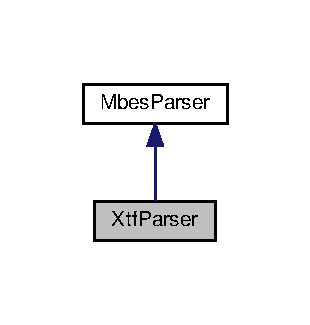
\includegraphics[width=149pt]{classXtfParser__inherit__graph}
\end{center}
\end{figure}


Graphe de collaboration de Xtf\+Parser\+:
\nopagebreak
\begin{figure}[H]
\begin{center}
\leavevmode
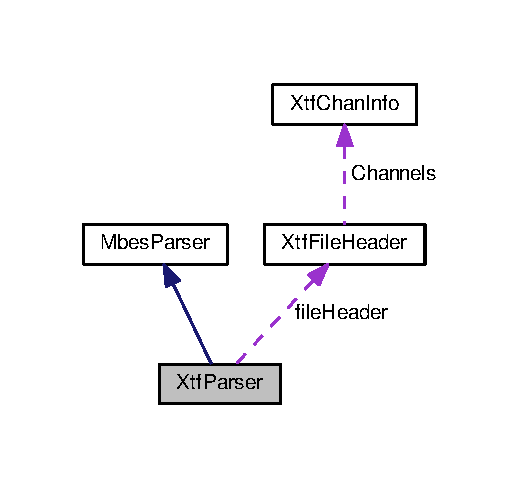
\includegraphics[width=251pt]{classXtfParser__coll__graph}
\end{center}
\end{figure}
\subsection*{Fonctions membres publiques}
\begin{DoxyCompactItemize}
\item 
\hyperlink{classXtfParser_a7de4082b13254ad7db07a6b2d5ec1580}{Xtf\+Parser} ()
\item 
\hyperlink{classXtfParser_a97fd350f03421815e5371142da30d440}{$\sim$\+Xtf\+Parser} ()
\item 
void \hyperlink{classXtfParser_ab123eca9033ded892f7dab148257db12}{parse} (std\+::string \&filename)
\item 
int \hyperlink{classXtfParser_a9d9d875429479e3d837860365f120969}{get\+Total\+Number\+Of\+Channels} ()
\item 
void \hyperlink{classXtfParser_ae8932c52b4030f14acd8b4419037c3eb}{process\+Ping} (uint64\+\_\+t micro\+Epoch, long id, double beam\+Angle, double tilt\+Angle, double two\+Way\+Travel\+Time, uint32\+\_\+t quality, uint32\+\_\+t intensity)
\item 
void \hyperlink{classXtfParser_a0fd79d938b6556f028330bba8513a32f}{process\+Attitude} (uint64\+\_\+t micro\+Epoch, float heading, float pitch, float roll)
\item 
void \hyperlink{classXtfParser_abbb02ef84a6f01696fb1f6ed23d2bb5f}{process\+Position} (uint64\+\_\+t micro\+Epoch, double longitude, double latitude, double height)
\item 
void \hyperlink{classXtfParser_a27d3b28415cd8e7f52bbc94fa39d9533}{process\+Swath\+Start} (double sound\+Velocity)
\end{DoxyCompactItemize}
\subsection*{Fonctions membres protégées}
\begin{DoxyCompactItemize}
\item 
void \hyperlink{classXtfParser_a7115b43a3325220a4119f1f1c087a83b}{process\+Packet\+Header} (\hyperlink{structXtfPacketHeader}{Xtf\+Packet\+Header} \&hdr)
\item 
void \hyperlink{classXtfParser_a5fde05f1fd275c683f445f3cb9384757}{process\+Packet} (\hyperlink{structXtfPacketHeader}{Xtf\+Packet\+Header} \&hdr, unsigned char $\ast$packet)
\item 
void \hyperlink{classXtfParser_a933ceba950e674e638b7d60629883668}{process\+Ping\+Header} (\hyperlink{structXtfPingHeader}{Xtf\+Ping\+Header} \&hdr)
\item 
void \hyperlink{classXtfParser_ad8c238e6c7e5f6ede01abbd42cf252ac}{process\+File\+Header} (\hyperlink{structXtfFileHeader}{Xtf\+File\+Header} \&hdr)
\item 
void \hyperlink{classXtfParser_a56bb25e017d5139f837b3ca24d98085f}{process\+Chan\+Info} (\hyperlink{structXtfChanInfo}{Xtf\+Chan\+Info} \&c)
\end{DoxyCompactItemize}
\subsection*{Attributs protégés}
\begin{DoxyCompactItemize}
\item 
\hyperlink{structXtfFileHeader}{Xtf\+File\+Header} \hyperlink{classXtfParser_a6ae47b7023578a93dfecbf3035fd9918}{file\+Header}
\end{DoxyCompactItemize}


\subsection{Description détaillée}
\begin{DoxyAuthor}{Auteur}
Guillaume Morissette
\end{DoxyAuthor}
Lit un fichier X\+TF et appelle un ensemble de callbacks pour chacun des types de datagrammes Par defaut, les callbacks ne font qu\textquotesingle{}imprimer les informations de celui-\/ci. Une application pourra surcharger celles-\/ci afin d\textquotesingle{}effectuer des operations specialisees. 

\subsection{Documentation des constructeurs et destructeur}
\mbox{\Hypertarget{classXtfParser_a7de4082b13254ad7db07a6b2d5ec1580}\label{classXtfParser_a7de4082b13254ad7db07a6b2d5ec1580}} 
\index{Xtf\+Parser@{Xtf\+Parser}!Xtf\+Parser@{Xtf\+Parser}}
\index{Xtf\+Parser@{Xtf\+Parser}!Xtf\+Parser@{Xtf\+Parser}}
\subsubsection{\texorpdfstring{Xtf\+Parser()}{XtfParser()}}
{\footnotesize\ttfamily Xtf\+Parser\+::\+Xtf\+Parser (\begin{DoxyParamCaption}{ }\end{DoxyParamCaption})}

\mbox{\Hypertarget{classXtfParser_a97fd350f03421815e5371142da30d440}\label{classXtfParser_a97fd350f03421815e5371142da30d440}} 
\index{Xtf\+Parser@{Xtf\+Parser}!````~Xtf\+Parser@{$\sim$\+Xtf\+Parser}}
\index{````~Xtf\+Parser@{$\sim$\+Xtf\+Parser}!Xtf\+Parser@{Xtf\+Parser}}
\subsubsection{\texorpdfstring{$\sim$\+Xtf\+Parser()}{~XtfParser()}}
{\footnotesize\ttfamily Xtf\+Parser\+::$\sim$\+Xtf\+Parser (\begin{DoxyParamCaption}{ }\end{DoxyParamCaption})}



\subsection{Documentation des fonctions membres}
\mbox{\Hypertarget{classXtfParser_a9d9d875429479e3d837860365f120969}\label{classXtfParser_a9d9d875429479e3d837860365f120969}} 
\index{Xtf\+Parser@{Xtf\+Parser}!get\+Total\+Number\+Of\+Channels@{get\+Total\+Number\+Of\+Channels}}
\index{get\+Total\+Number\+Of\+Channels@{get\+Total\+Number\+Of\+Channels}!Xtf\+Parser@{Xtf\+Parser}}
\subsubsection{\texorpdfstring{get\+Total\+Number\+Of\+Channels()}{getTotalNumberOfChannels()}}
{\footnotesize\ttfamily int Xtf\+Parser\+::get\+Total\+Number\+Of\+Channels (\begin{DoxyParamCaption}{ }\end{DoxyParamCaption})}

\mbox{\Hypertarget{classXtfParser_ab123eca9033ded892f7dab148257db12}\label{classXtfParser_ab123eca9033ded892f7dab148257db12}} 
\index{Xtf\+Parser@{Xtf\+Parser}!parse@{parse}}
\index{parse@{parse}!Xtf\+Parser@{Xtf\+Parser}}
\subsubsection{\texorpdfstring{parse()}{parse()}}
{\footnotesize\ttfamily void Xtf\+Parser\+::parse (\begin{DoxyParamCaption}\item[{std\+::string \&}]{filename }\end{DoxyParamCaption})}

\mbox{\Hypertarget{classXtfParser_a0fd79d938b6556f028330bba8513a32f}\label{classXtfParser_a0fd79d938b6556f028330bba8513a32f}} 
\index{Xtf\+Parser@{Xtf\+Parser}!process\+Attitude@{process\+Attitude}}
\index{process\+Attitude@{process\+Attitude}!Xtf\+Parser@{Xtf\+Parser}}
\subsubsection{\texorpdfstring{process\+Attitude()}{processAttitude()}}
{\footnotesize\ttfamily void Xtf\+Parser\+::process\+Attitude (\begin{DoxyParamCaption}\item[{uint64\+\_\+t}]{micro\+Epoch,  }\item[{float}]{heading,  }\item[{float}]{pitch,  }\item[{float}]{roll }\end{DoxyParamCaption})}

\mbox{\Hypertarget{classXtfParser_a56bb25e017d5139f837b3ca24d98085f}\label{classXtfParser_a56bb25e017d5139f837b3ca24d98085f}} 
\index{Xtf\+Parser@{Xtf\+Parser}!process\+Chan\+Info@{process\+Chan\+Info}}
\index{process\+Chan\+Info@{process\+Chan\+Info}!Xtf\+Parser@{Xtf\+Parser}}
\subsubsection{\texorpdfstring{process\+Chan\+Info()}{processChanInfo()}}
{\footnotesize\ttfamily void Xtf\+Parser\+::process\+Chan\+Info (\begin{DoxyParamCaption}\item[{\hyperlink{structXtfChanInfo}{Xtf\+Chan\+Info} \&}]{c }\end{DoxyParamCaption})\hspace{0.3cm}{\ttfamily [protected]}}

\mbox{\Hypertarget{classXtfParser_ad8c238e6c7e5f6ede01abbd42cf252ac}\label{classXtfParser_ad8c238e6c7e5f6ede01abbd42cf252ac}} 
\index{Xtf\+Parser@{Xtf\+Parser}!process\+File\+Header@{process\+File\+Header}}
\index{process\+File\+Header@{process\+File\+Header}!Xtf\+Parser@{Xtf\+Parser}}
\subsubsection{\texorpdfstring{process\+File\+Header()}{processFileHeader()}}
{\footnotesize\ttfamily void Xtf\+Parser\+::process\+File\+Header (\begin{DoxyParamCaption}\item[{\hyperlink{structXtfFileHeader}{Xtf\+File\+Header} \&}]{hdr }\end{DoxyParamCaption})\hspace{0.3cm}{\ttfamily [protected]}}

\mbox{\Hypertarget{classXtfParser_a5fde05f1fd275c683f445f3cb9384757}\label{classXtfParser_a5fde05f1fd275c683f445f3cb9384757}} 
\index{Xtf\+Parser@{Xtf\+Parser}!process\+Packet@{process\+Packet}}
\index{process\+Packet@{process\+Packet}!Xtf\+Parser@{Xtf\+Parser}}
\subsubsection{\texorpdfstring{process\+Packet()}{processPacket()}}
{\footnotesize\ttfamily void Xtf\+Parser\+::process\+Packet (\begin{DoxyParamCaption}\item[{\hyperlink{structXtfPacketHeader}{Xtf\+Packet\+Header} \&}]{hdr,  }\item[{unsigned char $\ast$}]{packet }\end{DoxyParamCaption})\hspace{0.3cm}{\ttfamily [protected]}}

\mbox{\Hypertarget{classXtfParser_a7115b43a3325220a4119f1f1c087a83b}\label{classXtfParser_a7115b43a3325220a4119f1f1c087a83b}} 
\index{Xtf\+Parser@{Xtf\+Parser}!process\+Packet\+Header@{process\+Packet\+Header}}
\index{process\+Packet\+Header@{process\+Packet\+Header}!Xtf\+Parser@{Xtf\+Parser}}
\subsubsection{\texorpdfstring{process\+Packet\+Header()}{processPacketHeader()}}
{\footnotesize\ttfamily void Xtf\+Parser\+::process\+Packet\+Header (\begin{DoxyParamCaption}\item[{\hyperlink{structXtfPacketHeader}{Xtf\+Packet\+Header} \&}]{hdr }\end{DoxyParamCaption})\hspace{0.3cm}{\ttfamily [protected]}}

\mbox{\Hypertarget{classXtfParser_ae8932c52b4030f14acd8b4419037c3eb}\label{classXtfParser_ae8932c52b4030f14acd8b4419037c3eb}} 
\index{Xtf\+Parser@{Xtf\+Parser}!process\+Ping@{process\+Ping}}
\index{process\+Ping@{process\+Ping}!Xtf\+Parser@{Xtf\+Parser}}
\subsubsection{\texorpdfstring{process\+Ping()}{processPing()}}
{\footnotesize\ttfamily void Xtf\+Parser\+::process\+Ping (\begin{DoxyParamCaption}\item[{uint64\+\_\+t}]{micro\+Epoch,  }\item[{long}]{id,  }\item[{double}]{beam\+Angle,  }\item[{double}]{tilt\+Angle,  }\item[{double}]{two\+Way\+Travel\+Time,  }\item[{uint32\+\_\+t}]{quality,  }\item[{uint32\+\_\+t}]{intensity }\end{DoxyParamCaption})\hspace{0.3cm}{\ttfamily [virtual]}}



Réimplémentée à partir de \hyperlink{classMbesParser_a9c099ea1003fff3c99991c37da1d40a6}{Mbes\+Parser}.

\mbox{\Hypertarget{classXtfParser_a933ceba950e674e638b7d60629883668}\label{classXtfParser_a933ceba950e674e638b7d60629883668}} 
\index{Xtf\+Parser@{Xtf\+Parser}!process\+Ping\+Header@{process\+Ping\+Header}}
\index{process\+Ping\+Header@{process\+Ping\+Header}!Xtf\+Parser@{Xtf\+Parser}}
\subsubsection{\texorpdfstring{process\+Ping\+Header()}{processPingHeader()}}
{\footnotesize\ttfamily void Xtf\+Parser\+::process\+Ping\+Header (\begin{DoxyParamCaption}\item[{\hyperlink{structXtfPingHeader}{Xtf\+Ping\+Header} \&}]{hdr }\end{DoxyParamCaption})\hspace{0.3cm}{\ttfamily [protected]}}

\mbox{\Hypertarget{classXtfParser_abbb02ef84a6f01696fb1f6ed23d2bb5f}\label{classXtfParser_abbb02ef84a6f01696fb1f6ed23d2bb5f}} 
\index{Xtf\+Parser@{Xtf\+Parser}!process\+Position@{process\+Position}}
\index{process\+Position@{process\+Position}!Xtf\+Parser@{Xtf\+Parser}}
\subsubsection{\texorpdfstring{process\+Position()}{processPosition()}}
{\footnotesize\ttfamily void Xtf\+Parser\+::process\+Position (\begin{DoxyParamCaption}\item[{uint64\+\_\+t}]{micro\+Epoch,  }\item[{double}]{longitude,  }\item[{double}]{latitude,  }\item[{double}]{height }\end{DoxyParamCaption})\hspace{0.3cm}{\ttfamily [virtual]}}



Réimplémentée à partir de \hyperlink{classMbesParser_add86a02726482d3a8e2a8aaf7f4beefa}{Mbes\+Parser}.

\mbox{\Hypertarget{classXtfParser_a27d3b28415cd8e7f52bbc94fa39d9533}\label{classXtfParser_a27d3b28415cd8e7f52bbc94fa39d9533}} 
\index{Xtf\+Parser@{Xtf\+Parser}!process\+Swath\+Start@{process\+Swath\+Start}}
\index{process\+Swath\+Start@{process\+Swath\+Start}!Xtf\+Parser@{Xtf\+Parser}}
\subsubsection{\texorpdfstring{process\+Swath\+Start()}{processSwathStart()}}
{\footnotesize\ttfamily void Xtf\+Parser\+::process\+Swath\+Start (\begin{DoxyParamCaption}\item[{double}]{sound\+Velocity }\end{DoxyParamCaption})}



\subsection{Documentation des données membres}
\mbox{\Hypertarget{classXtfParser_a6ae47b7023578a93dfecbf3035fd9918}\label{classXtfParser_a6ae47b7023578a93dfecbf3035fd9918}} 
\index{Xtf\+Parser@{Xtf\+Parser}!file\+Header@{file\+Header}}
\index{file\+Header@{file\+Header}!Xtf\+Parser@{Xtf\+Parser}}
\subsubsection{\texorpdfstring{file\+Header}{fileHeader}}
{\footnotesize\ttfamily \hyperlink{structXtfFileHeader}{Xtf\+File\+Header} Xtf\+Parser\+::file\+Header\hspace{0.3cm}{\ttfamily [protected]}}



La documentation de cette classe a été générée à partir du fichier suivant \+:\begin{DoxyCompactItemize}
\item 
src/datagrams/xtf/\hyperlink{XtfParser_8hpp}{Xtf\+Parser.\+hpp}\end{DoxyCompactItemize}

\hypertarget{structXtfPingChanHeader}{}\section{Référence de la structure Xtf\+Ping\+Chan\+Header}
\label{structXtfPingChanHeader}\index{Xtf\+Ping\+Chan\+Header@{Xtf\+Ping\+Chan\+Header}}


{\ttfamily \#include $<$Xtf\+Types.\+hpp$>$}

\subsection*{Attributs publics}
\begin{DoxyCompactItemize}
\item 
uint16\+\_\+t \hyperlink{structXtfPingChanHeader_ab2103654e24128c1f6541de84a8b9fb6}{Channel\+Number}
\item 
uint16\+\_\+t \hyperlink{structXtfPingChanHeader_a882db6e8a67ea919da17d890b2986022}{Downsample\+Method}
\item 
float \hyperlink{structXtfPingChanHeader_ac1fa5b82e755e59106e63cc1151404e4}{Slant\+Range}
\item 
float \hyperlink{structXtfPingChanHeader_a05befa73f6c02c6e7a4b8b647323bc1a}{Ground\+Range}
\item 
float \hyperlink{structXtfPingChanHeader_a667a4f19b2afb8cca48765d4a34d4906}{Time\+Delay}
\item 
float \hyperlink{structXtfPingChanHeader_ac74621607feab6bb035f0593941168d5}{Time\+Duration}
\item 
float \hyperlink{structXtfPingChanHeader_aca227333ab99ec454d585674bf5ef2ab}{Seconds\+Per\+Ping}
\item 
uint16\+\_\+t \hyperlink{structXtfPingChanHeader_a901e35315fbd81de608627ccb1303a6b}{Processing\+Flags}
\item 
uint16\+\_\+t \hyperlink{structXtfPingChanHeader_a13a02d3eef47befb893aa28194388034}{Frequency}
\item 
uint16\+\_\+t \hyperlink{structXtfPingChanHeader_a52b9bb8252b294545cc790e7e3970fd8}{Initial\+Gain\+Code}
\item 
uint16\+\_\+t \hyperlink{structXtfPingChanHeader_aa60ed3a085d6df63e764dcdc8856cf09}{Gain\+Code}
\item 
uint16\+\_\+t \hyperlink{structXtfPingChanHeader_a999a25f718223c0406f897570adb864f}{Band\+Width}
\item 
uint32\+\_\+t \hyperlink{structXtfPingChanHeader_a155ecf1c56f503251d95f5dd518447a3}{Contact\+Number}
\item 
uint16\+\_\+t \hyperlink{structXtfPingChanHeader_ac5295a152c2918a4a6b03716c381532b}{Contact\+Classification}
\item 
uint8\+\_\+t \hyperlink{structXtfPingChanHeader_afbbf1dcb5a945ab1d534a012fc0773d5}{Contact\+Sub\+Number}
\item 
uint8\+\_\+t \hyperlink{structXtfPingChanHeader_adbdbbb9f0ab433cabfedd9e1b36938b7}{Contact\+Type}
\item 
uint32\+\_\+t \hyperlink{structXtfPingChanHeader_a6aaaa540e66aaaddcb56e152c91a8652}{Num\+Samples}
\item 
uint16\+\_\+t \hyperlink{structXtfPingChanHeader_a969098397e500698a856a6ee0ba754f8}{Millivolt\+Scale}
\item 
float \hyperlink{structXtfPingChanHeader_ae570c68d6b2688a2aafd9650db9f0b96}{Contact\+Time\+Off\+Track}
\item 
uint8\+\_\+t \hyperlink{structXtfPingChanHeader_a38117b0c4bf9f9d29c8fb141eaa6ab42}{Contact\+Close\+Number}
\item 
uint8\+\_\+t \hyperlink{structXtfPingChanHeader_ad02669fb0f9899028661efc979734cfd}{Reserved2}
\item 
float \hyperlink{structXtfPingChanHeader_a7b52780ea2ec665924e2afedb8c47810}{Fixed\+V\+S\+OP}
\item 
int16\+\_\+t \hyperlink{structXtfPingChanHeader_a7f1b535bf81c110abea3862c6cf71e6b}{Weight}
\item 
uint8\+\_\+t \hyperlink{structXtfPingChanHeader_a56a6ea21690593dd164b0276fc988d94}{Reserved\+Space} \mbox{[}4\mbox{]}
\end{DoxyCompactItemize}


\subsection{Documentation des données membres}
\mbox{\Hypertarget{structXtfPingChanHeader_a999a25f718223c0406f897570adb864f}\label{structXtfPingChanHeader_a999a25f718223c0406f897570adb864f}} 
\index{Xtf\+Ping\+Chan\+Header@{Xtf\+Ping\+Chan\+Header}!Band\+Width@{Band\+Width}}
\index{Band\+Width@{Band\+Width}!Xtf\+Ping\+Chan\+Header@{Xtf\+Ping\+Chan\+Header}}
\subsubsection{\texorpdfstring{Band\+Width}{BandWidth}}
{\footnotesize\ttfamily uint16\+\_\+t Xtf\+Ping\+Chan\+Header\+::\+Band\+Width}

\mbox{\Hypertarget{structXtfPingChanHeader_ab2103654e24128c1f6541de84a8b9fb6}\label{structXtfPingChanHeader_ab2103654e24128c1f6541de84a8b9fb6}} 
\index{Xtf\+Ping\+Chan\+Header@{Xtf\+Ping\+Chan\+Header}!Channel\+Number@{Channel\+Number}}
\index{Channel\+Number@{Channel\+Number}!Xtf\+Ping\+Chan\+Header@{Xtf\+Ping\+Chan\+Header}}
\subsubsection{\texorpdfstring{Channel\+Number}{ChannelNumber}}
{\footnotesize\ttfamily uint16\+\_\+t Xtf\+Ping\+Chan\+Header\+::\+Channel\+Number}

\mbox{\Hypertarget{structXtfPingChanHeader_ac5295a152c2918a4a6b03716c381532b}\label{structXtfPingChanHeader_ac5295a152c2918a4a6b03716c381532b}} 
\index{Xtf\+Ping\+Chan\+Header@{Xtf\+Ping\+Chan\+Header}!Contact\+Classification@{Contact\+Classification}}
\index{Contact\+Classification@{Contact\+Classification}!Xtf\+Ping\+Chan\+Header@{Xtf\+Ping\+Chan\+Header}}
\subsubsection{\texorpdfstring{Contact\+Classification}{ContactClassification}}
{\footnotesize\ttfamily uint16\+\_\+t Xtf\+Ping\+Chan\+Header\+::\+Contact\+Classification}

\mbox{\Hypertarget{structXtfPingChanHeader_a38117b0c4bf9f9d29c8fb141eaa6ab42}\label{structXtfPingChanHeader_a38117b0c4bf9f9d29c8fb141eaa6ab42}} 
\index{Xtf\+Ping\+Chan\+Header@{Xtf\+Ping\+Chan\+Header}!Contact\+Close\+Number@{Contact\+Close\+Number}}
\index{Contact\+Close\+Number@{Contact\+Close\+Number}!Xtf\+Ping\+Chan\+Header@{Xtf\+Ping\+Chan\+Header}}
\subsubsection{\texorpdfstring{Contact\+Close\+Number}{ContactCloseNumber}}
{\footnotesize\ttfamily uint8\+\_\+t Xtf\+Ping\+Chan\+Header\+::\+Contact\+Close\+Number}

\mbox{\Hypertarget{structXtfPingChanHeader_a155ecf1c56f503251d95f5dd518447a3}\label{structXtfPingChanHeader_a155ecf1c56f503251d95f5dd518447a3}} 
\index{Xtf\+Ping\+Chan\+Header@{Xtf\+Ping\+Chan\+Header}!Contact\+Number@{Contact\+Number}}
\index{Contact\+Number@{Contact\+Number}!Xtf\+Ping\+Chan\+Header@{Xtf\+Ping\+Chan\+Header}}
\subsubsection{\texorpdfstring{Contact\+Number}{ContactNumber}}
{\footnotesize\ttfamily uint32\+\_\+t Xtf\+Ping\+Chan\+Header\+::\+Contact\+Number}

\mbox{\Hypertarget{structXtfPingChanHeader_afbbf1dcb5a945ab1d534a012fc0773d5}\label{structXtfPingChanHeader_afbbf1dcb5a945ab1d534a012fc0773d5}} 
\index{Xtf\+Ping\+Chan\+Header@{Xtf\+Ping\+Chan\+Header}!Contact\+Sub\+Number@{Contact\+Sub\+Number}}
\index{Contact\+Sub\+Number@{Contact\+Sub\+Number}!Xtf\+Ping\+Chan\+Header@{Xtf\+Ping\+Chan\+Header}}
\subsubsection{\texorpdfstring{Contact\+Sub\+Number}{ContactSubNumber}}
{\footnotesize\ttfamily uint8\+\_\+t Xtf\+Ping\+Chan\+Header\+::\+Contact\+Sub\+Number}

\mbox{\Hypertarget{structXtfPingChanHeader_ae570c68d6b2688a2aafd9650db9f0b96}\label{structXtfPingChanHeader_ae570c68d6b2688a2aafd9650db9f0b96}} 
\index{Xtf\+Ping\+Chan\+Header@{Xtf\+Ping\+Chan\+Header}!Contact\+Time\+Off\+Track@{Contact\+Time\+Off\+Track}}
\index{Contact\+Time\+Off\+Track@{Contact\+Time\+Off\+Track}!Xtf\+Ping\+Chan\+Header@{Xtf\+Ping\+Chan\+Header}}
\subsubsection{\texorpdfstring{Contact\+Time\+Off\+Track}{ContactTimeOffTrack}}
{\footnotesize\ttfamily float Xtf\+Ping\+Chan\+Header\+::\+Contact\+Time\+Off\+Track}

\mbox{\Hypertarget{structXtfPingChanHeader_adbdbbb9f0ab433cabfedd9e1b36938b7}\label{structXtfPingChanHeader_adbdbbb9f0ab433cabfedd9e1b36938b7}} 
\index{Xtf\+Ping\+Chan\+Header@{Xtf\+Ping\+Chan\+Header}!Contact\+Type@{Contact\+Type}}
\index{Contact\+Type@{Contact\+Type}!Xtf\+Ping\+Chan\+Header@{Xtf\+Ping\+Chan\+Header}}
\subsubsection{\texorpdfstring{Contact\+Type}{ContactType}}
{\footnotesize\ttfamily uint8\+\_\+t Xtf\+Ping\+Chan\+Header\+::\+Contact\+Type}

\mbox{\Hypertarget{structXtfPingChanHeader_a882db6e8a67ea919da17d890b2986022}\label{structXtfPingChanHeader_a882db6e8a67ea919da17d890b2986022}} 
\index{Xtf\+Ping\+Chan\+Header@{Xtf\+Ping\+Chan\+Header}!Downsample\+Method@{Downsample\+Method}}
\index{Downsample\+Method@{Downsample\+Method}!Xtf\+Ping\+Chan\+Header@{Xtf\+Ping\+Chan\+Header}}
\subsubsection{\texorpdfstring{Downsample\+Method}{DownsampleMethod}}
{\footnotesize\ttfamily uint16\+\_\+t Xtf\+Ping\+Chan\+Header\+::\+Downsample\+Method}

\mbox{\Hypertarget{structXtfPingChanHeader_a7b52780ea2ec665924e2afedb8c47810}\label{structXtfPingChanHeader_a7b52780ea2ec665924e2afedb8c47810}} 
\index{Xtf\+Ping\+Chan\+Header@{Xtf\+Ping\+Chan\+Header}!Fixed\+V\+S\+OP@{Fixed\+V\+S\+OP}}
\index{Fixed\+V\+S\+OP@{Fixed\+V\+S\+OP}!Xtf\+Ping\+Chan\+Header@{Xtf\+Ping\+Chan\+Header}}
\subsubsection{\texorpdfstring{Fixed\+V\+S\+OP}{FixedVSOP}}
{\footnotesize\ttfamily float Xtf\+Ping\+Chan\+Header\+::\+Fixed\+V\+S\+OP}

\mbox{\Hypertarget{structXtfPingChanHeader_a13a02d3eef47befb893aa28194388034}\label{structXtfPingChanHeader_a13a02d3eef47befb893aa28194388034}} 
\index{Xtf\+Ping\+Chan\+Header@{Xtf\+Ping\+Chan\+Header}!Frequency@{Frequency}}
\index{Frequency@{Frequency}!Xtf\+Ping\+Chan\+Header@{Xtf\+Ping\+Chan\+Header}}
\subsubsection{\texorpdfstring{Frequency}{Frequency}}
{\footnotesize\ttfamily uint16\+\_\+t Xtf\+Ping\+Chan\+Header\+::\+Frequency}

\mbox{\Hypertarget{structXtfPingChanHeader_aa60ed3a085d6df63e764dcdc8856cf09}\label{structXtfPingChanHeader_aa60ed3a085d6df63e764dcdc8856cf09}} 
\index{Xtf\+Ping\+Chan\+Header@{Xtf\+Ping\+Chan\+Header}!Gain\+Code@{Gain\+Code}}
\index{Gain\+Code@{Gain\+Code}!Xtf\+Ping\+Chan\+Header@{Xtf\+Ping\+Chan\+Header}}
\subsubsection{\texorpdfstring{Gain\+Code}{GainCode}}
{\footnotesize\ttfamily uint16\+\_\+t Xtf\+Ping\+Chan\+Header\+::\+Gain\+Code}

\mbox{\Hypertarget{structXtfPingChanHeader_a05befa73f6c02c6e7a4b8b647323bc1a}\label{structXtfPingChanHeader_a05befa73f6c02c6e7a4b8b647323bc1a}} 
\index{Xtf\+Ping\+Chan\+Header@{Xtf\+Ping\+Chan\+Header}!Ground\+Range@{Ground\+Range}}
\index{Ground\+Range@{Ground\+Range}!Xtf\+Ping\+Chan\+Header@{Xtf\+Ping\+Chan\+Header}}
\subsubsection{\texorpdfstring{Ground\+Range}{GroundRange}}
{\footnotesize\ttfamily float Xtf\+Ping\+Chan\+Header\+::\+Ground\+Range}

\mbox{\Hypertarget{structXtfPingChanHeader_a52b9bb8252b294545cc790e7e3970fd8}\label{structXtfPingChanHeader_a52b9bb8252b294545cc790e7e3970fd8}} 
\index{Xtf\+Ping\+Chan\+Header@{Xtf\+Ping\+Chan\+Header}!Initial\+Gain\+Code@{Initial\+Gain\+Code}}
\index{Initial\+Gain\+Code@{Initial\+Gain\+Code}!Xtf\+Ping\+Chan\+Header@{Xtf\+Ping\+Chan\+Header}}
\subsubsection{\texorpdfstring{Initial\+Gain\+Code}{InitialGainCode}}
{\footnotesize\ttfamily uint16\+\_\+t Xtf\+Ping\+Chan\+Header\+::\+Initial\+Gain\+Code}

\mbox{\Hypertarget{structXtfPingChanHeader_a969098397e500698a856a6ee0ba754f8}\label{structXtfPingChanHeader_a969098397e500698a856a6ee0ba754f8}} 
\index{Xtf\+Ping\+Chan\+Header@{Xtf\+Ping\+Chan\+Header}!Millivolt\+Scale@{Millivolt\+Scale}}
\index{Millivolt\+Scale@{Millivolt\+Scale}!Xtf\+Ping\+Chan\+Header@{Xtf\+Ping\+Chan\+Header}}
\subsubsection{\texorpdfstring{Millivolt\+Scale}{MillivoltScale}}
{\footnotesize\ttfamily uint16\+\_\+t Xtf\+Ping\+Chan\+Header\+::\+Millivolt\+Scale}

\mbox{\Hypertarget{structXtfPingChanHeader_a6aaaa540e66aaaddcb56e152c91a8652}\label{structXtfPingChanHeader_a6aaaa540e66aaaddcb56e152c91a8652}} 
\index{Xtf\+Ping\+Chan\+Header@{Xtf\+Ping\+Chan\+Header}!Num\+Samples@{Num\+Samples}}
\index{Num\+Samples@{Num\+Samples}!Xtf\+Ping\+Chan\+Header@{Xtf\+Ping\+Chan\+Header}}
\subsubsection{\texorpdfstring{Num\+Samples}{NumSamples}}
{\footnotesize\ttfamily uint32\+\_\+t Xtf\+Ping\+Chan\+Header\+::\+Num\+Samples}

\mbox{\Hypertarget{structXtfPingChanHeader_a901e35315fbd81de608627ccb1303a6b}\label{structXtfPingChanHeader_a901e35315fbd81de608627ccb1303a6b}} 
\index{Xtf\+Ping\+Chan\+Header@{Xtf\+Ping\+Chan\+Header}!Processing\+Flags@{Processing\+Flags}}
\index{Processing\+Flags@{Processing\+Flags}!Xtf\+Ping\+Chan\+Header@{Xtf\+Ping\+Chan\+Header}}
\subsubsection{\texorpdfstring{Processing\+Flags}{ProcessingFlags}}
{\footnotesize\ttfamily uint16\+\_\+t Xtf\+Ping\+Chan\+Header\+::\+Processing\+Flags}

\mbox{\Hypertarget{structXtfPingChanHeader_ad02669fb0f9899028661efc979734cfd}\label{structXtfPingChanHeader_ad02669fb0f9899028661efc979734cfd}} 
\index{Xtf\+Ping\+Chan\+Header@{Xtf\+Ping\+Chan\+Header}!Reserved2@{Reserved2}}
\index{Reserved2@{Reserved2}!Xtf\+Ping\+Chan\+Header@{Xtf\+Ping\+Chan\+Header}}
\subsubsection{\texorpdfstring{Reserved2}{Reserved2}}
{\footnotesize\ttfamily uint8\+\_\+t Xtf\+Ping\+Chan\+Header\+::\+Reserved2}

\mbox{\Hypertarget{structXtfPingChanHeader_a56a6ea21690593dd164b0276fc988d94}\label{structXtfPingChanHeader_a56a6ea21690593dd164b0276fc988d94}} 
\index{Xtf\+Ping\+Chan\+Header@{Xtf\+Ping\+Chan\+Header}!Reserved\+Space@{Reserved\+Space}}
\index{Reserved\+Space@{Reserved\+Space}!Xtf\+Ping\+Chan\+Header@{Xtf\+Ping\+Chan\+Header}}
\subsubsection{\texorpdfstring{Reserved\+Space}{ReservedSpace}}
{\footnotesize\ttfamily uint8\+\_\+t Xtf\+Ping\+Chan\+Header\+::\+Reserved\+Space\mbox{[}4\mbox{]}}

\mbox{\Hypertarget{structXtfPingChanHeader_aca227333ab99ec454d585674bf5ef2ab}\label{structXtfPingChanHeader_aca227333ab99ec454d585674bf5ef2ab}} 
\index{Xtf\+Ping\+Chan\+Header@{Xtf\+Ping\+Chan\+Header}!Seconds\+Per\+Ping@{Seconds\+Per\+Ping}}
\index{Seconds\+Per\+Ping@{Seconds\+Per\+Ping}!Xtf\+Ping\+Chan\+Header@{Xtf\+Ping\+Chan\+Header}}
\subsubsection{\texorpdfstring{Seconds\+Per\+Ping}{SecondsPerPing}}
{\footnotesize\ttfamily float Xtf\+Ping\+Chan\+Header\+::\+Seconds\+Per\+Ping}

\mbox{\Hypertarget{structXtfPingChanHeader_ac1fa5b82e755e59106e63cc1151404e4}\label{structXtfPingChanHeader_ac1fa5b82e755e59106e63cc1151404e4}} 
\index{Xtf\+Ping\+Chan\+Header@{Xtf\+Ping\+Chan\+Header}!Slant\+Range@{Slant\+Range}}
\index{Slant\+Range@{Slant\+Range}!Xtf\+Ping\+Chan\+Header@{Xtf\+Ping\+Chan\+Header}}
\subsubsection{\texorpdfstring{Slant\+Range}{SlantRange}}
{\footnotesize\ttfamily float Xtf\+Ping\+Chan\+Header\+::\+Slant\+Range}

\mbox{\Hypertarget{structXtfPingChanHeader_a667a4f19b2afb8cca48765d4a34d4906}\label{structXtfPingChanHeader_a667a4f19b2afb8cca48765d4a34d4906}} 
\index{Xtf\+Ping\+Chan\+Header@{Xtf\+Ping\+Chan\+Header}!Time\+Delay@{Time\+Delay}}
\index{Time\+Delay@{Time\+Delay}!Xtf\+Ping\+Chan\+Header@{Xtf\+Ping\+Chan\+Header}}
\subsubsection{\texorpdfstring{Time\+Delay}{TimeDelay}}
{\footnotesize\ttfamily float Xtf\+Ping\+Chan\+Header\+::\+Time\+Delay}

\mbox{\Hypertarget{structXtfPingChanHeader_ac74621607feab6bb035f0593941168d5}\label{structXtfPingChanHeader_ac74621607feab6bb035f0593941168d5}} 
\index{Xtf\+Ping\+Chan\+Header@{Xtf\+Ping\+Chan\+Header}!Time\+Duration@{Time\+Duration}}
\index{Time\+Duration@{Time\+Duration}!Xtf\+Ping\+Chan\+Header@{Xtf\+Ping\+Chan\+Header}}
\subsubsection{\texorpdfstring{Time\+Duration}{TimeDuration}}
{\footnotesize\ttfamily float Xtf\+Ping\+Chan\+Header\+::\+Time\+Duration}

\mbox{\Hypertarget{structXtfPingChanHeader_a7f1b535bf81c110abea3862c6cf71e6b}\label{structXtfPingChanHeader_a7f1b535bf81c110abea3862c6cf71e6b}} 
\index{Xtf\+Ping\+Chan\+Header@{Xtf\+Ping\+Chan\+Header}!Weight@{Weight}}
\index{Weight@{Weight}!Xtf\+Ping\+Chan\+Header@{Xtf\+Ping\+Chan\+Header}}
\subsubsection{\texorpdfstring{Weight}{Weight}}
{\footnotesize\ttfamily int16\+\_\+t Xtf\+Ping\+Chan\+Header\+::\+Weight}



La documentation de cette structure a été générée à partir du fichier suivant \+:\begin{DoxyCompactItemize}
\item 
src/datagrams/xtf/\hyperlink{XtfTypes_8hpp}{Xtf\+Types.\+hpp}\end{DoxyCompactItemize}

\hypertarget{structXtfPingHeader}{}\section{Référence de la structure Xtf\+Ping\+Header}
\label{structXtfPingHeader}\index{Xtf\+Ping\+Header@{Xtf\+Ping\+Header}}


{\ttfamily \#include $<$Xtf\+Types.\+hpp$>$}

\subsection*{Attributs publics}
\begin{DoxyCompactItemize}
\item 
uint16\+\_\+t \hyperlink{structXtfPingHeader_a9cda24d1b0cc5ace7b9cba5b1f0caf85}{Year}
\item 
uint8\+\_\+t \hyperlink{structXtfPingHeader_a4886fadcf6fd6d13db542d07f7e23269}{Month}
\item 
uint8\+\_\+t \hyperlink{structXtfPingHeader_a94f7114684926ee407d7168a7d2bb104}{Day}
\item 
uint8\+\_\+t \hyperlink{structXtfPingHeader_acbf30dd1ebd8416ca4cc969f117c0854}{Hour}
\item 
uint8\+\_\+t \hyperlink{structXtfPingHeader_a3f34dac271fc6b2ed5618f49cd642d15}{Minute}
\item 
uint8\+\_\+t \hyperlink{structXtfPingHeader_a83d68cd9692b973fcd4412b319c9b1a8}{Second}
\item 
uint8\+\_\+t \hyperlink{structXtfPingHeader_ae1ac0020439ea0fb39f73c8689ae8791}{H\+Seconds}
\item 
uint16\+\_\+t \hyperlink{structXtfPingHeader_a8c3cd4f05edeb7de12307c7a7136ce33}{Julian\+Day}
\item 
uint32\+\_\+t \hyperlink{structXtfPingHeader_ad3ce92406211b07295786dbb6187d2a6}{Event\+Number}
\item 
uint32\+\_\+t \hyperlink{structXtfPingHeader_a22617daf03da6c0378d3832fe2275f58}{Ping\+Number}
\item 
float \hyperlink{structXtfPingHeader_a99d4cbd7eb9c74bb4a8fd2d85da1a499}{Sound\+Velocity}
\item 
float \hyperlink{structXtfPingHeader_a2da14eac074067bdb52d0e3cb8702dc4}{Ocean\+Tide}
\item 
uint32\+\_\+t \hyperlink{structXtfPingHeader_a412ddd8940a44731043661b69d6eb256}{Reserved2}
\item 
float \hyperlink{structXtfPingHeader_a0ebdbaa7e8dbe0107a023c03a18fd7b1}{Conductivity\+Freq}
\item 
float \hyperlink{structXtfPingHeader_a474ada8be75ec65928f154e7cc55faf2}{Temperature\+Freq}
\item 
float \hyperlink{structXtfPingHeader_a0e7f321d1c8f5020bb5932ce0eb00a44}{Pressure\+Freq}
\item 
float \hyperlink{structXtfPingHeader_aff7f3cea88f9e025ac02f74d55f19a0e}{Pressure\+Temp}
\item 
float \hyperlink{structXtfPingHeader_afe76e708e756c0d0332b8cca8634fa07}{Conductivity}
\item 
float \hyperlink{structXtfPingHeader_a995d67006342ba9fcf7f8dda3bf9ebaa}{Water\+Temperature}
\item 
float \hyperlink{structXtfPingHeader_a8a4d7151530b03a30c933898eff394fa}{Pressure}
\item 
float \hyperlink{structXtfPingHeader_a73b3838aec39b4a81fb9108534c626a6}{Computed\+Sound\+Velocity}
\item 
float \hyperlink{structXtfPingHeader_a04ee3c6b70d1500696574c067b095835}{MagX}
\item 
float \hyperlink{structXtfPingHeader_a54c4d16e15bc7c6b849474aa8fe17ea7}{MagY}
\item 
float \hyperlink{structXtfPingHeader_a32157ba735745ecc7db8d07f0e4a3f1a}{MagZ}
\item 
float \hyperlink{structXtfPingHeader_a86b13c0947d7c8e847c4cbabd19d66d0}{Aux\+Val1}
\item 
float \hyperlink{structXtfPingHeader_a4780de3bd4667ed9c3a9ea94523f0fae}{Aux\+Val2}
\item 
float \hyperlink{structXtfPingHeader_ac9d0ef6484b8f7eb4afa728ed168b41a}{Aux\+Val3}
\item 
float \hyperlink{structXtfPingHeader_ad64af804c96db0af3cc2648b6d8a4573}{Aux\+Val4}
\item 
float \hyperlink{structXtfPingHeader_ab4b11a1d4eae6b4d935b3d54855f1195}{Aux\+Val5}
\item 
float \hyperlink{structXtfPingHeader_a81c53a2d0484e494d9b891352334afce}{Aux\+Val6}
\item 
float \hyperlink{structXtfPingHeader_afaad7bea39b9b67d331b199243f1b23c}{Speed\+Log}
\item 
float \hyperlink{structXtfPingHeader_a8d889b3bd1af85962f4b0e3164fc715a}{Turbidity}
\item 
float \hyperlink{structXtfPingHeader_aab430dc0ebca788807b2dbdfdcd9d29f}{Ship\+Speed}
\item 
float \hyperlink{structXtfPingHeader_a2c7ec394192377c85013bf0519cd0e35}{Ship\+Gyro}
\item 
double \hyperlink{structXtfPingHeader_ab1a8a86c74041b26c3c57414a4334471}{Ship\+Ycoordinate}
\item 
double \hyperlink{structXtfPingHeader_ad0b2b9ce11483ac7cb2dae940adc2494}{Ship\+Xcoordinate}
\item 
uint16\+\_\+t \hyperlink{structXtfPingHeader_a91637a56cb34850d47f7affdff9ae967}{Ship\+Altitude}
\item 
uint16\+\_\+t \hyperlink{structXtfPingHeader_acfd6401290226590c1689128d1cd6c6a}{Ship\+Depth}
\item 
uint8\+\_\+t \hyperlink{structXtfPingHeader_a0acfacef5b080e9daaf0372fb2de0e8b}{Fix\+Time\+Hour}
\item 
uint8\+\_\+t \hyperlink{structXtfPingHeader_ab083bd57394263b12397c8998803c8d3}{Fix\+Time\+Minute}
\item 
uint8\+\_\+t \hyperlink{structXtfPingHeader_af0f1df7af2780f44a761088e39275f77}{Fix\+Time\+Second}
\item 
uint8\+\_\+t \hyperlink{structXtfPingHeader_a02193e8b01a4440498c2405bb239e39e}{Fix\+Time\+Hsecond}
\item 
float \hyperlink{structXtfPingHeader_a55322e3af7f8895c8fc493644715d21d}{Sensor\+Speed}
\item 
float \hyperlink{structXtfPingHeader_a52d43640d8029af34ec7bad88dc19bfd}{KP}
\item 
double \hyperlink{structXtfPingHeader_a2d51d2bd0532584e772d3a9d4fa4d09c}{Sensor\+Ycoordinate}
\item 
double \hyperlink{structXtfPingHeader_ac492dc2fe343118cad441c37c9c9e1d9}{Sensor\+Xcoordinate}
\item 
uint16\+\_\+t \hyperlink{structXtfPingHeader_a34f81bc6328cf5b2ca6fc95a5218c225}{Sonar\+Status}
\item 
uint16\+\_\+t \hyperlink{structXtfPingHeader_ab4d9254168e925706b8f086e1e4b0052}{Range\+To\+Fish}
\item 
uint16\+\_\+t \hyperlink{structXtfPingHeader_ac80b2d492aa47cde1d5f2e5ee2ef4d2b}{Bearing\+To\+Fish}
\item 
uint16\+\_\+t \hyperlink{structXtfPingHeader_a2aedefaeb24eb43b69e0499a8ad40ebc}{Cable\+Out}
\item 
float \hyperlink{structXtfPingHeader_aa495554086770426cfc8b906b54d6150}{Layback}
\item 
float \hyperlink{structXtfPingHeader_acdc978a55b0a9d8b1bc3180e86b203d3}{Cable\+Tension}
\item 
float \hyperlink{structXtfPingHeader_a5fb2a907631646b772c4795d09efa298}{Sensor\+Depth}
\item 
float \hyperlink{structXtfPingHeader_a9b6bd368e97d2d3e00ce5bba7abf30d0}{Sensor\+Primary\+Altitude}
\item 
float \hyperlink{structXtfPingHeader_a3c60c1f42c53e3533c08a93a3fee027b}{Sensor\+Aux\+Altitude}
\item 
float \hyperlink{structXtfPingHeader_aa3dbc632d9429a3638b3ebffeb8f2e64}{Sensor\+Pitch}
\item 
float \hyperlink{structXtfPingHeader_a0aa89112bcb5a598ea575adb63e392c5}{Sensor\+Roll}
\item 
float \hyperlink{structXtfPingHeader_af8dc29cd8b8989d596433139b3fd66a1}{Sensor\+Heading}
\item 
float \hyperlink{structXtfPingHeader_a82e649a277ebefc678002f2f35a9ed1a}{Heave}
\item 
float \hyperlink{structXtfPingHeader_a705d9bcf0415f5c2138b83e0d865b528}{Yaw}
\item 
uint32\+\_\+t \hyperlink{structXtfPingHeader_ad60f19c7449cfb2569dddcbb93da7042}{Attitude\+Time\+Tag}
\item 
float \hyperlink{structXtfPingHeader_a48229392bb4ccc8bdc35e8f2a19cc363}{D\+OT}
\item 
uint32\+\_\+t \hyperlink{structXtfPingHeader_a5475582e52b52f56416b5a4ee93b5e92}{Nav\+Fix\+Milliseconds}
\item 
uint8\+\_\+t \hyperlink{structXtfPingHeader_ac7e8ed5281deee113f91b7339e0babbd}{Computer\+Clock\+Hour}
\item 
uint8\+\_\+t \hyperlink{structXtfPingHeader_a4ffa1e429080763b4e405cdc389af671}{Computer\+Clock\+Minute}
\item 
uint8\+\_\+t \hyperlink{structXtfPingHeader_a3953292e24a019093dfa8a423b803268}{Computer\+Clock\+Second}
\item 
uint8\+\_\+t \hyperlink{structXtfPingHeader_a5f864caca5f651aaf4377c2609d9dab7}{Computer\+Clock\+Hsec}
\item 
short \hyperlink{structXtfPingHeader_a84994ace0bc0e1c776355d7739b9f93d}{Fish\+Position\+DeltaX}
\item 
short \hyperlink{structXtfPingHeader_a100011d222312bc4177490e6b36f9de4}{Fish\+Position\+DeltaY}
\item 
unsigned char \hyperlink{structXtfPingHeader_a7990fd8fa82298bc812014a14cad74ff}{Fish\+Position\+Error\+Code}
\item 
unsigned int \hyperlink{structXtfPingHeader_a5a03b90aab99da9f6b2ff3cb384fd859}{Optional\+Offsey}
\item 
uint8\+\_\+t \hyperlink{structXtfPingHeader_a29adedb19cbbd3f9096038bc8e8c7bb4}{Cable\+Out\+Hundredths}
\item 
uint8\+\_\+t \hyperlink{structXtfPingHeader_ab2405648890a0cc720da8bf0adbecd0f}{Reserved\+Space2} \mbox{[}6\mbox{]}
\end{DoxyCompactItemize}


\subsection{Documentation des données membres}
\mbox{\Hypertarget{structXtfPingHeader_ad60f19c7449cfb2569dddcbb93da7042}\label{structXtfPingHeader_ad60f19c7449cfb2569dddcbb93da7042}} 
\index{Xtf\+Ping\+Header@{Xtf\+Ping\+Header}!Attitude\+Time\+Tag@{Attitude\+Time\+Tag}}
\index{Attitude\+Time\+Tag@{Attitude\+Time\+Tag}!Xtf\+Ping\+Header@{Xtf\+Ping\+Header}}
\subsubsection{\texorpdfstring{Attitude\+Time\+Tag}{AttitudeTimeTag}}
{\footnotesize\ttfamily uint32\+\_\+t Xtf\+Ping\+Header\+::\+Attitude\+Time\+Tag}

\mbox{\Hypertarget{structXtfPingHeader_a86b13c0947d7c8e847c4cbabd19d66d0}\label{structXtfPingHeader_a86b13c0947d7c8e847c4cbabd19d66d0}} 
\index{Xtf\+Ping\+Header@{Xtf\+Ping\+Header}!Aux\+Val1@{Aux\+Val1}}
\index{Aux\+Val1@{Aux\+Val1}!Xtf\+Ping\+Header@{Xtf\+Ping\+Header}}
\subsubsection{\texorpdfstring{Aux\+Val1}{AuxVal1}}
{\footnotesize\ttfamily float Xtf\+Ping\+Header\+::\+Aux\+Val1}

\mbox{\Hypertarget{structXtfPingHeader_a4780de3bd4667ed9c3a9ea94523f0fae}\label{structXtfPingHeader_a4780de3bd4667ed9c3a9ea94523f0fae}} 
\index{Xtf\+Ping\+Header@{Xtf\+Ping\+Header}!Aux\+Val2@{Aux\+Val2}}
\index{Aux\+Val2@{Aux\+Val2}!Xtf\+Ping\+Header@{Xtf\+Ping\+Header}}
\subsubsection{\texorpdfstring{Aux\+Val2}{AuxVal2}}
{\footnotesize\ttfamily float Xtf\+Ping\+Header\+::\+Aux\+Val2}

\mbox{\Hypertarget{structXtfPingHeader_ac9d0ef6484b8f7eb4afa728ed168b41a}\label{structXtfPingHeader_ac9d0ef6484b8f7eb4afa728ed168b41a}} 
\index{Xtf\+Ping\+Header@{Xtf\+Ping\+Header}!Aux\+Val3@{Aux\+Val3}}
\index{Aux\+Val3@{Aux\+Val3}!Xtf\+Ping\+Header@{Xtf\+Ping\+Header}}
\subsubsection{\texorpdfstring{Aux\+Val3}{AuxVal3}}
{\footnotesize\ttfamily float Xtf\+Ping\+Header\+::\+Aux\+Val3}

\mbox{\Hypertarget{structXtfPingHeader_ad64af804c96db0af3cc2648b6d8a4573}\label{structXtfPingHeader_ad64af804c96db0af3cc2648b6d8a4573}} 
\index{Xtf\+Ping\+Header@{Xtf\+Ping\+Header}!Aux\+Val4@{Aux\+Val4}}
\index{Aux\+Val4@{Aux\+Val4}!Xtf\+Ping\+Header@{Xtf\+Ping\+Header}}
\subsubsection{\texorpdfstring{Aux\+Val4}{AuxVal4}}
{\footnotesize\ttfamily float Xtf\+Ping\+Header\+::\+Aux\+Val4}

\mbox{\Hypertarget{structXtfPingHeader_ab4b11a1d4eae6b4d935b3d54855f1195}\label{structXtfPingHeader_ab4b11a1d4eae6b4d935b3d54855f1195}} 
\index{Xtf\+Ping\+Header@{Xtf\+Ping\+Header}!Aux\+Val5@{Aux\+Val5}}
\index{Aux\+Val5@{Aux\+Val5}!Xtf\+Ping\+Header@{Xtf\+Ping\+Header}}
\subsubsection{\texorpdfstring{Aux\+Val5}{AuxVal5}}
{\footnotesize\ttfamily float Xtf\+Ping\+Header\+::\+Aux\+Val5}

\mbox{\Hypertarget{structXtfPingHeader_a81c53a2d0484e494d9b891352334afce}\label{structXtfPingHeader_a81c53a2d0484e494d9b891352334afce}} 
\index{Xtf\+Ping\+Header@{Xtf\+Ping\+Header}!Aux\+Val6@{Aux\+Val6}}
\index{Aux\+Val6@{Aux\+Val6}!Xtf\+Ping\+Header@{Xtf\+Ping\+Header}}
\subsubsection{\texorpdfstring{Aux\+Val6}{AuxVal6}}
{\footnotesize\ttfamily float Xtf\+Ping\+Header\+::\+Aux\+Val6}

\mbox{\Hypertarget{structXtfPingHeader_ac80b2d492aa47cde1d5f2e5ee2ef4d2b}\label{structXtfPingHeader_ac80b2d492aa47cde1d5f2e5ee2ef4d2b}} 
\index{Xtf\+Ping\+Header@{Xtf\+Ping\+Header}!Bearing\+To\+Fish@{Bearing\+To\+Fish}}
\index{Bearing\+To\+Fish@{Bearing\+To\+Fish}!Xtf\+Ping\+Header@{Xtf\+Ping\+Header}}
\subsubsection{\texorpdfstring{Bearing\+To\+Fish}{BearingToFish}}
{\footnotesize\ttfamily uint16\+\_\+t Xtf\+Ping\+Header\+::\+Bearing\+To\+Fish}

\mbox{\Hypertarget{structXtfPingHeader_a2aedefaeb24eb43b69e0499a8ad40ebc}\label{structXtfPingHeader_a2aedefaeb24eb43b69e0499a8ad40ebc}} 
\index{Xtf\+Ping\+Header@{Xtf\+Ping\+Header}!Cable\+Out@{Cable\+Out}}
\index{Cable\+Out@{Cable\+Out}!Xtf\+Ping\+Header@{Xtf\+Ping\+Header}}
\subsubsection{\texorpdfstring{Cable\+Out}{CableOut}}
{\footnotesize\ttfamily uint16\+\_\+t Xtf\+Ping\+Header\+::\+Cable\+Out}

\mbox{\Hypertarget{structXtfPingHeader_a29adedb19cbbd3f9096038bc8e8c7bb4}\label{structXtfPingHeader_a29adedb19cbbd3f9096038bc8e8c7bb4}} 
\index{Xtf\+Ping\+Header@{Xtf\+Ping\+Header}!Cable\+Out\+Hundredths@{Cable\+Out\+Hundredths}}
\index{Cable\+Out\+Hundredths@{Cable\+Out\+Hundredths}!Xtf\+Ping\+Header@{Xtf\+Ping\+Header}}
\subsubsection{\texorpdfstring{Cable\+Out\+Hundredths}{CableOutHundredths}}
{\footnotesize\ttfamily uint8\+\_\+t Xtf\+Ping\+Header\+::\+Cable\+Out\+Hundredths}

\mbox{\Hypertarget{structXtfPingHeader_acdc978a55b0a9d8b1bc3180e86b203d3}\label{structXtfPingHeader_acdc978a55b0a9d8b1bc3180e86b203d3}} 
\index{Xtf\+Ping\+Header@{Xtf\+Ping\+Header}!Cable\+Tension@{Cable\+Tension}}
\index{Cable\+Tension@{Cable\+Tension}!Xtf\+Ping\+Header@{Xtf\+Ping\+Header}}
\subsubsection{\texorpdfstring{Cable\+Tension}{CableTension}}
{\footnotesize\ttfamily float Xtf\+Ping\+Header\+::\+Cable\+Tension}

\mbox{\Hypertarget{structXtfPingHeader_a73b3838aec39b4a81fb9108534c626a6}\label{structXtfPingHeader_a73b3838aec39b4a81fb9108534c626a6}} 
\index{Xtf\+Ping\+Header@{Xtf\+Ping\+Header}!Computed\+Sound\+Velocity@{Computed\+Sound\+Velocity}}
\index{Computed\+Sound\+Velocity@{Computed\+Sound\+Velocity}!Xtf\+Ping\+Header@{Xtf\+Ping\+Header}}
\subsubsection{\texorpdfstring{Computed\+Sound\+Velocity}{ComputedSoundVelocity}}
{\footnotesize\ttfamily float Xtf\+Ping\+Header\+::\+Computed\+Sound\+Velocity}

\mbox{\Hypertarget{structXtfPingHeader_ac7e8ed5281deee113f91b7339e0babbd}\label{structXtfPingHeader_ac7e8ed5281deee113f91b7339e0babbd}} 
\index{Xtf\+Ping\+Header@{Xtf\+Ping\+Header}!Computer\+Clock\+Hour@{Computer\+Clock\+Hour}}
\index{Computer\+Clock\+Hour@{Computer\+Clock\+Hour}!Xtf\+Ping\+Header@{Xtf\+Ping\+Header}}
\subsubsection{\texorpdfstring{Computer\+Clock\+Hour}{ComputerClockHour}}
{\footnotesize\ttfamily uint8\+\_\+t Xtf\+Ping\+Header\+::\+Computer\+Clock\+Hour}

\mbox{\Hypertarget{structXtfPingHeader_a5f864caca5f651aaf4377c2609d9dab7}\label{structXtfPingHeader_a5f864caca5f651aaf4377c2609d9dab7}} 
\index{Xtf\+Ping\+Header@{Xtf\+Ping\+Header}!Computer\+Clock\+Hsec@{Computer\+Clock\+Hsec}}
\index{Computer\+Clock\+Hsec@{Computer\+Clock\+Hsec}!Xtf\+Ping\+Header@{Xtf\+Ping\+Header}}
\subsubsection{\texorpdfstring{Computer\+Clock\+Hsec}{ComputerClockHsec}}
{\footnotesize\ttfamily uint8\+\_\+t Xtf\+Ping\+Header\+::\+Computer\+Clock\+Hsec}

\mbox{\Hypertarget{structXtfPingHeader_a4ffa1e429080763b4e405cdc389af671}\label{structXtfPingHeader_a4ffa1e429080763b4e405cdc389af671}} 
\index{Xtf\+Ping\+Header@{Xtf\+Ping\+Header}!Computer\+Clock\+Minute@{Computer\+Clock\+Minute}}
\index{Computer\+Clock\+Minute@{Computer\+Clock\+Minute}!Xtf\+Ping\+Header@{Xtf\+Ping\+Header}}
\subsubsection{\texorpdfstring{Computer\+Clock\+Minute}{ComputerClockMinute}}
{\footnotesize\ttfamily uint8\+\_\+t Xtf\+Ping\+Header\+::\+Computer\+Clock\+Minute}

\mbox{\Hypertarget{structXtfPingHeader_a3953292e24a019093dfa8a423b803268}\label{structXtfPingHeader_a3953292e24a019093dfa8a423b803268}} 
\index{Xtf\+Ping\+Header@{Xtf\+Ping\+Header}!Computer\+Clock\+Second@{Computer\+Clock\+Second}}
\index{Computer\+Clock\+Second@{Computer\+Clock\+Second}!Xtf\+Ping\+Header@{Xtf\+Ping\+Header}}
\subsubsection{\texorpdfstring{Computer\+Clock\+Second}{ComputerClockSecond}}
{\footnotesize\ttfamily uint8\+\_\+t Xtf\+Ping\+Header\+::\+Computer\+Clock\+Second}

\mbox{\Hypertarget{structXtfPingHeader_afe76e708e756c0d0332b8cca8634fa07}\label{structXtfPingHeader_afe76e708e756c0d0332b8cca8634fa07}} 
\index{Xtf\+Ping\+Header@{Xtf\+Ping\+Header}!Conductivity@{Conductivity}}
\index{Conductivity@{Conductivity}!Xtf\+Ping\+Header@{Xtf\+Ping\+Header}}
\subsubsection{\texorpdfstring{Conductivity}{Conductivity}}
{\footnotesize\ttfamily float Xtf\+Ping\+Header\+::\+Conductivity}

\mbox{\Hypertarget{structXtfPingHeader_a0ebdbaa7e8dbe0107a023c03a18fd7b1}\label{structXtfPingHeader_a0ebdbaa7e8dbe0107a023c03a18fd7b1}} 
\index{Xtf\+Ping\+Header@{Xtf\+Ping\+Header}!Conductivity\+Freq@{Conductivity\+Freq}}
\index{Conductivity\+Freq@{Conductivity\+Freq}!Xtf\+Ping\+Header@{Xtf\+Ping\+Header}}
\subsubsection{\texorpdfstring{Conductivity\+Freq}{ConductivityFreq}}
{\footnotesize\ttfamily float Xtf\+Ping\+Header\+::\+Conductivity\+Freq}

\mbox{\Hypertarget{structXtfPingHeader_a94f7114684926ee407d7168a7d2bb104}\label{structXtfPingHeader_a94f7114684926ee407d7168a7d2bb104}} 
\index{Xtf\+Ping\+Header@{Xtf\+Ping\+Header}!Day@{Day}}
\index{Day@{Day}!Xtf\+Ping\+Header@{Xtf\+Ping\+Header}}
\subsubsection{\texorpdfstring{Day}{Day}}
{\footnotesize\ttfamily uint8\+\_\+t Xtf\+Ping\+Header\+::\+Day}

\mbox{\Hypertarget{structXtfPingHeader_a48229392bb4ccc8bdc35e8f2a19cc363}\label{structXtfPingHeader_a48229392bb4ccc8bdc35e8f2a19cc363}} 
\index{Xtf\+Ping\+Header@{Xtf\+Ping\+Header}!D\+OT@{D\+OT}}
\index{D\+OT@{D\+OT}!Xtf\+Ping\+Header@{Xtf\+Ping\+Header}}
\subsubsection{\texorpdfstring{D\+OT}{DOT}}
{\footnotesize\ttfamily float Xtf\+Ping\+Header\+::\+D\+OT}

\mbox{\Hypertarget{structXtfPingHeader_ad3ce92406211b07295786dbb6187d2a6}\label{structXtfPingHeader_ad3ce92406211b07295786dbb6187d2a6}} 
\index{Xtf\+Ping\+Header@{Xtf\+Ping\+Header}!Event\+Number@{Event\+Number}}
\index{Event\+Number@{Event\+Number}!Xtf\+Ping\+Header@{Xtf\+Ping\+Header}}
\subsubsection{\texorpdfstring{Event\+Number}{EventNumber}}
{\footnotesize\ttfamily uint32\+\_\+t Xtf\+Ping\+Header\+::\+Event\+Number}

\mbox{\Hypertarget{structXtfPingHeader_a84994ace0bc0e1c776355d7739b9f93d}\label{structXtfPingHeader_a84994ace0bc0e1c776355d7739b9f93d}} 
\index{Xtf\+Ping\+Header@{Xtf\+Ping\+Header}!Fish\+Position\+DeltaX@{Fish\+Position\+DeltaX}}
\index{Fish\+Position\+DeltaX@{Fish\+Position\+DeltaX}!Xtf\+Ping\+Header@{Xtf\+Ping\+Header}}
\subsubsection{\texorpdfstring{Fish\+Position\+DeltaX}{FishPositionDeltaX}}
{\footnotesize\ttfamily short Xtf\+Ping\+Header\+::\+Fish\+Position\+DeltaX}

\mbox{\Hypertarget{structXtfPingHeader_a100011d222312bc4177490e6b36f9de4}\label{structXtfPingHeader_a100011d222312bc4177490e6b36f9de4}} 
\index{Xtf\+Ping\+Header@{Xtf\+Ping\+Header}!Fish\+Position\+DeltaY@{Fish\+Position\+DeltaY}}
\index{Fish\+Position\+DeltaY@{Fish\+Position\+DeltaY}!Xtf\+Ping\+Header@{Xtf\+Ping\+Header}}
\subsubsection{\texorpdfstring{Fish\+Position\+DeltaY}{FishPositionDeltaY}}
{\footnotesize\ttfamily short Xtf\+Ping\+Header\+::\+Fish\+Position\+DeltaY}

\mbox{\Hypertarget{structXtfPingHeader_a7990fd8fa82298bc812014a14cad74ff}\label{structXtfPingHeader_a7990fd8fa82298bc812014a14cad74ff}} 
\index{Xtf\+Ping\+Header@{Xtf\+Ping\+Header}!Fish\+Position\+Error\+Code@{Fish\+Position\+Error\+Code}}
\index{Fish\+Position\+Error\+Code@{Fish\+Position\+Error\+Code}!Xtf\+Ping\+Header@{Xtf\+Ping\+Header}}
\subsubsection{\texorpdfstring{Fish\+Position\+Error\+Code}{FishPositionErrorCode}}
{\footnotesize\ttfamily unsigned char Xtf\+Ping\+Header\+::\+Fish\+Position\+Error\+Code}

\mbox{\Hypertarget{structXtfPingHeader_a0acfacef5b080e9daaf0372fb2de0e8b}\label{structXtfPingHeader_a0acfacef5b080e9daaf0372fb2de0e8b}} 
\index{Xtf\+Ping\+Header@{Xtf\+Ping\+Header}!Fix\+Time\+Hour@{Fix\+Time\+Hour}}
\index{Fix\+Time\+Hour@{Fix\+Time\+Hour}!Xtf\+Ping\+Header@{Xtf\+Ping\+Header}}
\subsubsection{\texorpdfstring{Fix\+Time\+Hour}{FixTimeHour}}
{\footnotesize\ttfamily uint8\+\_\+t Xtf\+Ping\+Header\+::\+Fix\+Time\+Hour}

\mbox{\Hypertarget{structXtfPingHeader_a02193e8b01a4440498c2405bb239e39e}\label{structXtfPingHeader_a02193e8b01a4440498c2405bb239e39e}} 
\index{Xtf\+Ping\+Header@{Xtf\+Ping\+Header}!Fix\+Time\+Hsecond@{Fix\+Time\+Hsecond}}
\index{Fix\+Time\+Hsecond@{Fix\+Time\+Hsecond}!Xtf\+Ping\+Header@{Xtf\+Ping\+Header}}
\subsubsection{\texorpdfstring{Fix\+Time\+Hsecond}{FixTimeHsecond}}
{\footnotesize\ttfamily uint8\+\_\+t Xtf\+Ping\+Header\+::\+Fix\+Time\+Hsecond}

\mbox{\Hypertarget{structXtfPingHeader_ab083bd57394263b12397c8998803c8d3}\label{structXtfPingHeader_ab083bd57394263b12397c8998803c8d3}} 
\index{Xtf\+Ping\+Header@{Xtf\+Ping\+Header}!Fix\+Time\+Minute@{Fix\+Time\+Minute}}
\index{Fix\+Time\+Minute@{Fix\+Time\+Minute}!Xtf\+Ping\+Header@{Xtf\+Ping\+Header}}
\subsubsection{\texorpdfstring{Fix\+Time\+Minute}{FixTimeMinute}}
{\footnotesize\ttfamily uint8\+\_\+t Xtf\+Ping\+Header\+::\+Fix\+Time\+Minute}

\mbox{\Hypertarget{structXtfPingHeader_af0f1df7af2780f44a761088e39275f77}\label{structXtfPingHeader_af0f1df7af2780f44a761088e39275f77}} 
\index{Xtf\+Ping\+Header@{Xtf\+Ping\+Header}!Fix\+Time\+Second@{Fix\+Time\+Second}}
\index{Fix\+Time\+Second@{Fix\+Time\+Second}!Xtf\+Ping\+Header@{Xtf\+Ping\+Header}}
\subsubsection{\texorpdfstring{Fix\+Time\+Second}{FixTimeSecond}}
{\footnotesize\ttfamily uint8\+\_\+t Xtf\+Ping\+Header\+::\+Fix\+Time\+Second}

\mbox{\Hypertarget{structXtfPingHeader_a82e649a277ebefc678002f2f35a9ed1a}\label{structXtfPingHeader_a82e649a277ebefc678002f2f35a9ed1a}} 
\index{Xtf\+Ping\+Header@{Xtf\+Ping\+Header}!Heave@{Heave}}
\index{Heave@{Heave}!Xtf\+Ping\+Header@{Xtf\+Ping\+Header}}
\subsubsection{\texorpdfstring{Heave}{Heave}}
{\footnotesize\ttfamily float Xtf\+Ping\+Header\+::\+Heave}

\mbox{\Hypertarget{structXtfPingHeader_acbf30dd1ebd8416ca4cc969f117c0854}\label{structXtfPingHeader_acbf30dd1ebd8416ca4cc969f117c0854}} 
\index{Xtf\+Ping\+Header@{Xtf\+Ping\+Header}!Hour@{Hour}}
\index{Hour@{Hour}!Xtf\+Ping\+Header@{Xtf\+Ping\+Header}}
\subsubsection{\texorpdfstring{Hour}{Hour}}
{\footnotesize\ttfamily uint8\+\_\+t Xtf\+Ping\+Header\+::\+Hour}

\mbox{\Hypertarget{structXtfPingHeader_ae1ac0020439ea0fb39f73c8689ae8791}\label{structXtfPingHeader_ae1ac0020439ea0fb39f73c8689ae8791}} 
\index{Xtf\+Ping\+Header@{Xtf\+Ping\+Header}!H\+Seconds@{H\+Seconds}}
\index{H\+Seconds@{H\+Seconds}!Xtf\+Ping\+Header@{Xtf\+Ping\+Header}}
\subsubsection{\texorpdfstring{H\+Seconds}{HSeconds}}
{\footnotesize\ttfamily uint8\+\_\+t Xtf\+Ping\+Header\+::\+H\+Seconds}

\mbox{\Hypertarget{structXtfPingHeader_a8c3cd4f05edeb7de12307c7a7136ce33}\label{structXtfPingHeader_a8c3cd4f05edeb7de12307c7a7136ce33}} 
\index{Xtf\+Ping\+Header@{Xtf\+Ping\+Header}!Julian\+Day@{Julian\+Day}}
\index{Julian\+Day@{Julian\+Day}!Xtf\+Ping\+Header@{Xtf\+Ping\+Header}}
\subsubsection{\texorpdfstring{Julian\+Day}{JulianDay}}
{\footnotesize\ttfamily uint16\+\_\+t Xtf\+Ping\+Header\+::\+Julian\+Day}

\mbox{\Hypertarget{structXtfPingHeader_a52d43640d8029af34ec7bad88dc19bfd}\label{structXtfPingHeader_a52d43640d8029af34ec7bad88dc19bfd}} 
\index{Xtf\+Ping\+Header@{Xtf\+Ping\+Header}!KP@{KP}}
\index{KP@{KP}!Xtf\+Ping\+Header@{Xtf\+Ping\+Header}}
\subsubsection{\texorpdfstring{KP}{KP}}
{\footnotesize\ttfamily float Xtf\+Ping\+Header\+::\+KP}

\mbox{\Hypertarget{structXtfPingHeader_aa495554086770426cfc8b906b54d6150}\label{structXtfPingHeader_aa495554086770426cfc8b906b54d6150}} 
\index{Xtf\+Ping\+Header@{Xtf\+Ping\+Header}!Layback@{Layback}}
\index{Layback@{Layback}!Xtf\+Ping\+Header@{Xtf\+Ping\+Header}}
\subsubsection{\texorpdfstring{Layback}{Layback}}
{\footnotesize\ttfamily float Xtf\+Ping\+Header\+::\+Layback}

\mbox{\Hypertarget{structXtfPingHeader_a04ee3c6b70d1500696574c067b095835}\label{structXtfPingHeader_a04ee3c6b70d1500696574c067b095835}} 
\index{Xtf\+Ping\+Header@{Xtf\+Ping\+Header}!MagX@{MagX}}
\index{MagX@{MagX}!Xtf\+Ping\+Header@{Xtf\+Ping\+Header}}
\subsubsection{\texorpdfstring{MagX}{MagX}}
{\footnotesize\ttfamily float Xtf\+Ping\+Header\+::\+MagX}

\mbox{\Hypertarget{structXtfPingHeader_a54c4d16e15bc7c6b849474aa8fe17ea7}\label{structXtfPingHeader_a54c4d16e15bc7c6b849474aa8fe17ea7}} 
\index{Xtf\+Ping\+Header@{Xtf\+Ping\+Header}!MagY@{MagY}}
\index{MagY@{MagY}!Xtf\+Ping\+Header@{Xtf\+Ping\+Header}}
\subsubsection{\texorpdfstring{MagY}{MagY}}
{\footnotesize\ttfamily float Xtf\+Ping\+Header\+::\+MagY}

\mbox{\Hypertarget{structXtfPingHeader_a32157ba735745ecc7db8d07f0e4a3f1a}\label{structXtfPingHeader_a32157ba735745ecc7db8d07f0e4a3f1a}} 
\index{Xtf\+Ping\+Header@{Xtf\+Ping\+Header}!MagZ@{MagZ}}
\index{MagZ@{MagZ}!Xtf\+Ping\+Header@{Xtf\+Ping\+Header}}
\subsubsection{\texorpdfstring{MagZ}{MagZ}}
{\footnotesize\ttfamily float Xtf\+Ping\+Header\+::\+MagZ}

\mbox{\Hypertarget{structXtfPingHeader_a3f34dac271fc6b2ed5618f49cd642d15}\label{structXtfPingHeader_a3f34dac271fc6b2ed5618f49cd642d15}} 
\index{Xtf\+Ping\+Header@{Xtf\+Ping\+Header}!Minute@{Minute}}
\index{Minute@{Minute}!Xtf\+Ping\+Header@{Xtf\+Ping\+Header}}
\subsubsection{\texorpdfstring{Minute}{Minute}}
{\footnotesize\ttfamily uint8\+\_\+t Xtf\+Ping\+Header\+::\+Minute}

\mbox{\Hypertarget{structXtfPingHeader_a4886fadcf6fd6d13db542d07f7e23269}\label{structXtfPingHeader_a4886fadcf6fd6d13db542d07f7e23269}} 
\index{Xtf\+Ping\+Header@{Xtf\+Ping\+Header}!Month@{Month}}
\index{Month@{Month}!Xtf\+Ping\+Header@{Xtf\+Ping\+Header}}
\subsubsection{\texorpdfstring{Month}{Month}}
{\footnotesize\ttfamily uint8\+\_\+t Xtf\+Ping\+Header\+::\+Month}

\mbox{\Hypertarget{structXtfPingHeader_a5475582e52b52f56416b5a4ee93b5e92}\label{structXtfPingHeader_a5475582e52b52f56416b5a4ee93b5e92}} 
\index{Xtf\+Ping\+Header@{Xtf\+Ping\+Header}!Nav\+Fix\+Milliseconds@{Nav\+Fix\+Milliseconds}}
\index{Nav\+Fix\+Milliseconds@{Nav\+Fix\+Milliseconds}!Xtf\+Ping\+Header@{Xtf\+Ping\+Header}}
\subsubsection{\texorpdfstring{Nav\+Fix\+Milliseconds}{NavFixMilliseconds}}
{\footnotesize\ttfamily uint32\+\_\+t Xtf\+Ping\+Header\+::\+Nav\+Fix\+Milliseconds}

\mbox{\Hypertarget{structXtfPingHeader_a2da14eac074067bdb52d0e3cb8702dc4}\label{structXtfPingHeader_a2da14eac074067bdb52d0e3cb8702dc4}} 
\index{Xtf\+Ping\+Header@{Xtf\+Ping\+Header}!Ocean\+Tide@{Ocean\+Tide}}
\index{Ocean\+Tide@{Ocean\+Tide}!Xtf\+Ping\+Header@{Xtf\+Ping\+Header}}
\subsubsection{\texorpdfstring{Ocean\+Tide}{OceanTide}}
{\footnotesize\ttfamily float Xtf\+Ping\+Header\+::\+Ocean\+Tide}

\mbox{\Hypertarget{structXtfPingHeader_a5a03b90aab99da9f6b2ff3cb384fd859}\label{structXtfPingHeader_a5a03b90aab99da9f6b2ff3cb384fd859}} 
\index{Xtf\+Ping\+Header@{Xtf\+Ping\+Header}!Optional\+Offsey@{Optional\+Offsey}}
\index{Optional\+Offsey@{Optional\+Offsey}!Xtf\+Ping\+Header@{Xtf\+Ping\+Header}}
\subsubsection{\texorpdfstring{Optional\+Offsey}{OptionalOffsey}}
{\footnotesize\ttfamily unsigned int Xtf\+Ping\+Header\+::\+Optional\+Offsey}

\mbox{\Hypertarget{structXtfPingHeader_a22617daf03da6c0378d3832fe2275f58}\label{structXtfPingHeader_a22617daf03da6c0378d3832fe2275f58}} 
\index{Xtf\+Ping\+Header@{Xtf\+Ping\+Header}!Ping\+Number@{Ping\+Number}}
\index{Ping\+Number@{Ping\+Number}!Xtf\+Ping\+Header@{Xtf\+Ping\+Header}}
\subsubsection{\texorpdfstring{Ping\+Number}{PingNumber}}
{\footnotesize\ttfamily uint32\+\_\+t Xtf\+Ping\+Header\+::\+Ping\+Number}

\mbox{\Hypertarget{structXtfPingHeader_a8a4d7151530b03a30c933898eff394fa}\label{structXtfPingHeader_a8a4d7151530b03a30c933898eff394fa}} 
\index{Xtf\+Ping\+Header@{Xtf\+Ping\+Header}!Pressure@{Pressure}}
\index{Pressure@{Pressure}!Xtf\+Ping\+Header@{Xtf\+Ping\+Header}}
\subsubsection{\texorpdfstring{Pressure}{Pressure}}
{\footnotesize\ttfamily float Xtf\+Ping\+Header\+::\+Pressure}

\mbox{\Hypertarget{structXtfPingHeader_a0e7f321d1c8f5020bb5932ce0eb00a44}\label{structXtfPingHeader_a0e7f321d1c8f5020bb5932ce0eb00a44}} 
\index{Xtf\+Ping\+Header@{Xtf\+Ping\+Header}!Pressure\+Freq@{Pressure\+Freq}}
\index{Pressure\+Freq@{Pressure\+Freq}!Xtf\+Ping\+Header@{Xtf\+Ping\+Header}}
\subsubsection{\texorpdfstring{Pressure\+Freq}{PressureFreq}}
{\footnotesize\ttfamily float Xtf\+Ping\+Header\+::\+Pressure\+Freq}

\mbox{\Hypertarget{structXtfPingHeader_aff7f3cea88f9e025ac02f74d55f19a0e}\label{structXtfPingHeader_aff7f3cea88f9e025ac02f74d55f19a0e}} 
\index{Xtf\+Ping\+Header@{Xtf\+Ping\+Header}!Pressure\+Temp@{Pressure\+Temp}}
\index{Pressure\+Temp@{Pressure\+Temp}!Xtf\+Ping\+Header@{Xtf\+Ping\+Header}}
\subsubsection{\texorpdfstring{Pressure\+Temp}{PressureTemp}}
{\footnotesize\ttfamily float Xtf\+Ping\+Header\+::\+Pressure\+Temp}

\mbox{\Hypertarget{structXtfPingHeader_ab4d9254168e925706b8f086e1e4b0052}\label{structXtfPingHeader_ab4d9254168e925706b8f086e1e4b0052}} 
\index{Xtf\+Ping\+Header@{Xtf\+Ping\+Header}!Range\+To\+Fish@{Range\+To\+Fish}}
\index{Range\+To\+Fish@{Range\+To\+Fish}!Xtf\+Ping\+Header@{Xtf\+Ping\+Header}}
\subsubsection{\texorpdfstring{Range\+To\+Fish}{RangeToFish}}
{\footnotesize\ttfamily uint16\+\_\+t Xtf\+Ping\+Header\+::\+Range\+To\+Fish}

\mbox{\Hypertarget{structXtfPingHeader_a412ddd8940a44731043661b69d6eb256}\label{structXtfPingHeader_a412ddd8940a44731043661b69d6eb256}} 
\index{Xtf\+Ping\+Header@{Xtf\+Ping\+Header}!Reserved2@{Reserved2}}
\index{Reserved2@{Reserved2}!Xtf\+Ping\+Header@{Xtf\+Ping\+Header}}
\subsubsection{\texorpdfstring{Reserved2}{Reserved2}}
{\footnotesize\ttfamily uint32\+\_\+t Xtf\+Ping\+Header\+::\+Reserved2}

\mbox{\Hypertarget{structXtfPingHeader_ab2405648890a0cc720da8bf0adbecd0f}\label{structXtfPingHeader_ab2405648890a0cc720da8bf0adbecd0f}} 
\index{Xtf\+Ping\+Header@{Xtf\+Ping\+Header}!Reserved\+Space2@{Reserved\+Space2}}
\index{Reserved\+Space2@{Reserved\+Space2}!Xtf\+Ping\+Header@{Xtf\+Ping\+Header}}
\subsubsection{\texorpdfstring{Reserved\+Space2}{ReservedSpace2}}
{\footnotesize\ttfamily uint8\+\_\+t Xtf\+Ping\+Header\+::\+Reserved\+Space2\mbox{[}6\mbox{]}}

\mbox{\Hypertarget{structXtfPingHeader_a83d68cd9692b973fcd4412b319c9b1a8}\label{structXtfPingHeader_a83d68cd9692b973fcd4412b319c9b1a8}} 
\index{Xtf\+Ping\+Header@{Xtf\+Ping\+Header}!Second@{Second}}
\index{Second@{Second}!Xtf\+Ping\+Header@{Xtf\+Ping\+Header}}
\subsubsection{\texorpdfstring{Second}{Second}}
{\footnotesize\ttfamily uint8\+\_\+t Xtf\+Ping\+Header\+::\+Second}

\mbox{\Hypertarget{structXtfPingHeader_a3c60c1f42c53e3533c08a93a3fee027b}\label{structXtfPingHeader_a3c60c1f42c53e3533c08a93a3fee027b}} 
\index{Xtf\+Ping\+Header@{Xtf\+Ping\+Header}!Sensor\+Aux\+Altitude@{Sensor\+Aux\+Altitude}}
\index{Sensor\+Aux\+Altitude@{Sensor\+Aux\+Altitude}!Xtf\+Ping\+Header@{Xtf\+Ping\+Header}}
\subsubsection{\texorpdfstring{Sensor\+Aux\+Altitude}{SensorAuxAltitude}}
{\footnotesize\ttfamily float Xtf\+Ping\+Header\+::\+Sensor\+Aux\+Altitude}

\mbox{\Hypertarget{structXtfPingHeader_a5fb2a907631646b772c4795d09efa298}\label{structXtfPingHeader_a5fb2a907631646b772c4795d09efa298}} 
\index{Xtf\+Ping\+Header@{Xtf\+Ping\+Header}!Sensor\+Depth@{Sensor\+Depth}}
\index{Sensor\+Depth@{Sensor\+Depth}!Xtf\+Ping\+Header@{Xtf\+Ping\+Header}}
\subsubsection{\texorpdfstring{Sensor\+Depth}{SensorDepth}}
{\footnotesize\ttfamily float Xtf\+Ping\+Header\+::\+Sensor\+Depth}

\mbox{\Hypertarget{structXtfPingHeader_af8dc29cd8b8989d596433139b3fd66a1}\label{structXtfPingHeader_af8dc29cd8b8989d596433139b3fd66a1}} 
\index{Xtf\+Ping\+Header@{Xtf\+Ping\+Header}!Sensor\+Heading@{Sensor\+Heading}}
\index{Sensor\+Heading@{Sensor\+Heading}!Xtf\+Ping\+Header@{Xtf\+Ping\+Header}}
\subsubsection{\texorpdfstring{Sensor\+Heading}{SensorHeading}}
{\footnotesize\ttfamily float Xtf\+Ping\+Header\+::\+Sensor\+Heading}

\mbox{\Hypertarget{structXtfPingHeader_aa3dbc632d9429a3638b3ebffeb8f2e64}\label{structXtfPingHeader_aa3dbc632d9429a3638b3ebffeb8f2e64}} 
\index{Xtf\+Ping\+Header@{Xtf\+Ping\+Header}!Sensor\+Pitch@{Sensor\+Pitch}}
\index{Sensor\+Pitch@{Sensor\+Pitch}!Xtf\+Ping\+Header@{Xtf\+Ping\+Header}}
\subsubsection{\texorpdfstring{Sensor\+Pitch}{SensorPitch}}
{\footnotesize\ttfamily float Xtf\+Ping\+Header\+::\+Sensor\+Pitch}

\mbox{\Hypertarget{structXtfPingHeader_a9b6bd368e97d2d3e00ce5bba7abf30d0}\label{structXtfPingHeader_a9b6bd368e97d2d3e00ce5bba7abf30d0}} 
\index{Xtf\+Ping\+Header@{Xtf\+Ping\+Header}!Sensor\+Primary\+Altitude@{Sensor\+Primary\+Altitude}}
\index{Sensor\+Primary\+Altitude@{Sensor\+Primary\+Altitude}!Xtf\+Ping\+Header@{Xtf\+Ping\+Header}}
\subsubsection{\texorpdfstring{Sensor\+Primary\+Altitude}{SensorPrimaryAltitude}}
{\footnotesize\ttfamily float Xtf\+Ping\+Header\+::\+Sensor\+Primary\+Altitude}

\mbox{\Hypertarget{structXtfPingHeader_a0aa89112bcb5a598ea575adb63e392c5}\label{structXtfPingHeader_a0aa89112bcb5a598ea575adb63e392c5}} 
\index{Xtf\+Ping\+Header@{Xtf\+Ping\+Header}!Sensor\+Roll@{Sensor\+Roll}}
\index{Sensor\+Roll@{Sensor\+Roll}!Xtf\+Ping\+Header@{Xtf\+Ping\+Header}}
\subsubsection{\texorpdfstring{Sensor\+Roll}{SensorRoll}}
{\footnotesize\ttfamily float Xtf\+Ping\+Header\+::\+Sensor\+Roll}

\mbox{\Hypertarget{structXtfPingHeader_a55322e3af7f8895c8fc493644715d21d}\label{structXtfPingHeader_a55322e3af7f8895c8fc493644715d21d}} 
\index{Xtf\+Ping\+Header@{Xtf\+Ping\+Header}!Sensor\+Speed@{Sensor\+Speed}}
\index{Sensor\+Speed@{Sensor\+Speed}!Xtf\+Ping\+Header@{Xtf\+Ping\+Header}}
\subsubsection{\texorpdfstring{Sensor\+Speed}{SensorSpeed}}
{\footnotesize\ttfamily float Xtf\+Ping\+Header\+::\+Sensor\+Speed}

\mbox{\Hypertarget{structXtfPingHeader_ac492dc2fe343118cad441c37c9c9e1d9}\label{structXtfPingHeader_ac492dc2fe343118cad441c37c9c9e1d9}} 
\index{Xtf\+Ping\+Header@{Xtf\+Ping\+Header}!Sensor\+Xcoordinate@{Sensor\+Xcoordinate}}
\index{Sensor\+Xcoordinate@{Sensor\+Xcoordinate}!Xtf\+Ping\+Header@{Xtf\+Ping\+Header}}
\subsubsection{\texorpdfstring{Sensor\+Xcoordinate}{SensorXcoordinate}}
{\footnotesize\ttfamily double Xtf\+Ping\+Header\+::\+Sensor\+Xcoordinate}

\mbox{\Hypertarget{structXtfPingHeader_a2d51d2bd0532584e772d3a9d4fa4d09c}\label{structXtfPingHeader_a2d51d2bd0532584e772d3a9d4fa4d09c}} 
\index{Xtf\+Ping\+Header@{Xtf\+Ping\+Header}!Sensor\+Ycoordinate@{Sensor\+Ycoordinate}}
\index{Sensor\+Ycoordinate@{Sensor\+Ycoordinate}!Xtf\+Ping\+Header@{Xtf\+Ping\+Header}}
\subsubsection{\texorpdfstring{Sensor\+Ycoordinate}{SensorYcoordinate}}
{\footnotesize\ttfamily double Xtf\+Ping\+Header\+::\+Sensor\+Ycoordinate}

\mbox{\Hypertarget{structXtfPingHeader_a91637a56cb34850d47f7affdff9ae967}\label{structXtfPingHeader_a91637a56cb34850d47f7affdff9ae967}} 
\index{Xtf\+Ping\+Header@{Xtf\+Ping\+Header}!Ship\+Altitude@{Ship\+Altitude}}
\index{Ship\+Altitude@{Ship\+Altitude}!Xtf\+Ping\+Header@{Xtf\+Ping\+Header}}
\subsubsection{\texorpdfstring{Ship\+Altitude}{ShipAltitude}}
{\footnotesize\ttfamily uint16\+\_\+t Xtf\+Ping\+Header\+::\+Ship\+Altitude}

\mbox{\Hypertarget{structXtfPingHeader_acfd6401290226590c1689128d1cd6c6a}\label{structXtfPingHeader_acfd6401290226590c1689128d1cd6c6a}} 
\index{Xtf\+Ping\+Header@{Xtf\+Ping\+Header}!Ship\+Depth@{Ship\+Depth}}
\index{Ship\+Depth@{Ship\+Depth}!Xtf\+Ping\+Header@{Xtf\+Ping\+Header}}
\subsubsection{\texorpdfstring{Ship\+Depth}{ShipDepth}}
{\footnotesize\ttfamily uint16\+\_\+t Xtf\+Ping\+Header\+::\+Ship\+Depth}

\mbox{\Hypertarget{structXtfPingHeader_a2c7ec394192377c85013bf0519cd0e35}\label{structXtfPingHeader_a2c7ec394192377c85013bf0519cd0e35}} 
\index{Xtf\+Ping\+Header@{Xtf\+Ping\+Header}!Ship\+Gyro@{Ship\+Gyro}}
\index{Ship\+Gyro@{Ship\+Gyro}!Xtf\+Ping\+Header@{Xtf\+Ping\+Header}}
\subsubsection{\texorpdfstring{Ship\+Gyro}{ShipGyro}}
{\footnotesize\ttfamily float Xtf\+Ping\+Header\+::\+Ship\+Gyro}

\mbox{\Hypertarget{structXtfPingHeader_aab430dc0ebca788807b2dbdfdcd9d29f}\label{structXtfPingHeader_aab430dc0ebca788807b2dbdfdcd9d29f}} 
\index{Xtf\+Ping\+Header@{Xtf\+Ping\+Header}!Ship\+Speed@{Ship\+Speed}}
\index{Ship\+Speed@{Ship\+Speed}!Xtf\+Ping\+Header@{Xtf\+Ping\+Header}}
\subsubsection{\texorpdfstring{Ship\+Speed}{ShipSpeed}}
{\footnotesize\ttfamily float Xtf\+Ping\+Header\+::\+Ship\+Speed}

\mbox{\Hypertarget{structXtfPingHeader_ad0b2b9ce11483ac7cb2dae940adc2494}\label{structXtfPingHeader_ad0b2b9ce11483ac7cb2dae940adc2494}} 
\index{Xtf\+Ping\+Header@{Xtf\+Ping\+Header}!Ship\+Xcoordinate@{Ship\+Xcoordinate}}
\index{Ship\+Xcoordinate@{Ship\+Xcoordinate}!Xtf\+Ping\+Header@{Xtf\+Ping\+Header}}
\subsubsection{\texorpdfstring{Ship\+Xcoordinate}{ShipXcoordinate}}
{\footnotesize\ttfamily double Xtf\+Ping\+Header\+::\+Ship\+Xcoordinate}

\mbox{\Hypertarget{structXtfPingHeader_ab1a8a86c74041b26c3c57414a4334471}\label{structXtfPingHeader_ab1a8a86c74041b26c3c57414a4334471}} 
\index{Xtf\+Ping\+Header@{Xtf\+Ping\+Header}!Ship\+Ycoordinate@{Ship\+Ycoordinate}}
\index{Ship\+Ycoordinate@{Ship\+Ycoordinate}!Xtf\+Ping\+Header@{Xtf\+Ping\+Header}}
\subsubsection{\texorpdfstring{Ship\+Ycoordinate}{ShipYcoordinate}}
{\footnotesize\ttfamily double Xtf\+Ping\+Header\+::\+Ship\+Ycoordinate}

\mbox{\Hypertarget{structXtfPingHeader_a34f81bc6328cf5b2ca6fc95a5218c225}\label{structXtfPingHeader_a34f81bc6328cf5b2ca6fc95a5218c225}} 
\index{Xtf\+Ping\+Header@{Xtf\+Ping\+Header}!Sonar\+Status@{Sonar\+Status}}
\index{Sonar\+Status@{Sonar\+Status}!Xtf\+Ping\+Header@{Xtf\+Ping\+Header}}
\subsubsection{\texorpdfstring{Sonar\+Status}{SonarStatus}}
{\footnotesize\ttfamily uint16\+\_\+t Xtf\+Ping\+Header\+::\+Sonar\+Status}

\mbox{\Hypertarget{structXtfPingHeader_a99d4cbd7eb9c74bb4a8fd2d85da1a499}\label{structXtfPingHeader_a99d4cbd7eb9c74bb4a8fd2d85da1a499}} 
\index{Xtf\+Ping\+Header@{Xtf\+Ping\+Header}!Sound\+Velocity@{Sound\+Velocity}}
\index{Sound\+Velocity@{Sound\+Velocity}!Xtf\+Ping\+Header@{Xtf\+Ping\+Header}}
\subsubsection{\texorpdfstring{Sound\+Velocity}{SoundVelocity}}
{\footnotesize\ttfamily float Xtf\+Ping\+Header\+::\+Sound\+Velocity}

\mbox{\Hypertarget{structXtfPingHeader_afaad7bea39b9b67d331b199243f1b23c}\label{structXtfPingHeader_afaad7bea39b9b67d331b199243f1b23c}} 
\index{Xtf\+Ping\+Header@{Xtf\+Ping\+Header}!Speed\+Log@{Speed\+Log}}
\index{Speed\+Log@{Speed\+Log}!Xtf\+Ping\+Header@{Xtf\+Ping\+Header}}
\subsubsection{\texorpdfstring{Speed\+Log}{SpeedLog}}
{\footnotesize\ttfamily float Xtf\+Ping\+Header\+::\+Speed\+Log}

\mbox{\Hypertarget{structXtfPingHeader_a474ada8be75ec65928f154e7cc55faf2}\label{structXtfPingHeader_a474ada8be75ec65928f154e7cc55faf2}} 
\index{Xtf\+Ping\+Header@{Xtf\+Ping\+Header}!Temperature\+Freq@{Temperature\+Freq}}
\index{Temperature\+Freq@{Temperature\+Freq}!Xtf\+Ping\+Header@{Xtf\+Ping\+Header}}
\subsubsection{\texorpdfstring{Temperature\+Freq}{TemperatureFreq}}
{\footnotesize\ttfamily float Xtf\+Ping\+Header\+::\+Temperature\+Freq}

\mbox{\Hypertarget{structXtfPingHeader_a8d889b3bd1af85962f4b0e3164fc715a}\label{structXtfPingHeader_a8d889b3bd1af85962f4b0e3164fc715a}} 
\index{Xtf\+Ping\+Header@{Xtf\+Ping\+Header}!Turbidity@{Turbidity}}
\index{Turbidity@{Turbidity}!Xtf\+Ping\+Header@{Xtf\+Ping\+Header}}
\subsubsection{\texorpdfstring{Turbidity}{Turbidity}}
{\footnotesize\ttfamily float Xtf\+Ping\+Header\+::\+Turbidity}

\mbox{\Hypertarget{structXtfPingHeader_a995d67006342ba9fcf7f8dda3bf9ebaa}\label{structXtfPingHeader_a995d67006342ba9fcf7f8dda3bf9ebaa}} 
\index{Xtf\+Ping\+Header@{Xtf\+Ping\+Header}!Water\+Temperature@{Water\+Temperature}}
\index{Water\+Temperature@{Water\+Temperature}!Xtf\+Ping\+Header@{Xtf\+Ping\+Header}}
\subsubsection{\texorpdfstring{Water\+Temperature}{WaterTemperature}}
{\footnotesize\ttfamily float Xtf\+Ping\+Header\+::\+Water\+Temperature}

\mbox{\Hypertarget{structXtfPingHeader_a705d9bcf0415f5c2138b83e0d865b528}\label{structXtfPingHeader_a705d9bcf0415f5c2138b83e0d865b528}} 
\index{Xtf\+Ping\+Header@{Xtf\+Ping\+Header}!Yaw@{Yaw}}
\index{Yaw@{Yaw}!Xtf\+Ping\+Header@{Xtf\+Ping\+Header}}
\subsubsection{\texorpdfstring{Yaw}{Yaw}}
{\footnotesize\ttfamily float Xtf\+Ping\+Header\+::\+Yaw}

\mbox{\Hypertarget{structXtfPingHeader_a9cda24d1b0cc5ace7b9cba5b1f0caf85}\label{structXtfPingHeader_a9cda24d1b0cc5ace7b9cba5b1f0caf85}} 
\index{Xtf\+Ping\+Header@{Xtf\+Ping\+Header}!Year@{Year}}
\index{Year@{Year}!Xtf\+Ping\+Header@{Xtf\+Ping\+Header}}
\subsubsection{\texorpdfstring{Year}{Year}}
{\footnotesize\ttfamily uint16\+\_\+t Xtf\+Ping\+Header\+::\+Year}



La documentation de cette structure a été générée à partir du fichier suivant \+:\begin{DoxyCompactItemize}
\item 
src/datagrams/xtf/\hyperlink{XtfTypes_8hpp}{Xtf\+Types.\+hpp}\end{DoxyCompactItemize}

\hypertarget{structXtfPosRawNavigation}{}\section{Référence de la structure Xtf\+Pos\+Raw\+Navigation}
\label{structXtfPosRawNavigation}\index{Xtf\+Pos\+Raw\+Navigation@{Xtf\+Pos\+Raw\+Navigation}}


{\ttfamily \#include $<$Xtf\+Types.\+hpp$>$}

\subsection*{Attributs publics}
\begin{DoxyCompactItemize}
\item 
uint16\+\_\+t \hyperlink{structXtfPosRawNavigation_a2e0d32b5ebb8153b10b8865aadcbfc6a}{Year}
\item 
uint8\+\_\+t \hyperlink{structXtfPosRawNavigation_aa92e448530742a582e18d7c0af232df5}{Month}
\item 
uint8\+\_\+t \hyperlink{structXtfPosRawNavigation_aacc1cb8b7ff1a394a4921f2a0074f551}{Day}
\item 
uint8\+\_\+t \hyperlink{structXtfPosRawNavigation_a4e1507a38ce886aaad5a7f7025257a0d}{Hour}
\item 
uint8\+\_\+t \hyperlink{structXtfPosRawNavigation_a6c1b24898daf661f2485b30f84aa3329}{Minutes}
\item 
uint8\+\_\+t \hyperlink{structXtfPosRawNavigation_a937a58d418bc71b387192b164a2f494e}{Seconds}
\item 
uint16\+\_\+t \hyperlink{structXtfPosRawNavigation_a1c8375adbb055a89897c520de70386a3}{Micro\+Seconds}
\item 
double \hyperlink{structXtfPosRawNavigation_a27bba05bee4b9c2e926d76e69d90c479}{Raw\+Ycoordinate}
\item 
double \hyperlink{structXtfPosRawNavigation_a9ef5a7b17a396d5843f20e1c85035ec2}{Raw\+Xcoordinate}
\item 
double \hyperlink{structXtfPosRawNavigation_a0ad1cb103827d5e9473b10b67112fe4f}{Raw\+Altitude}
\item 
float \hyperlink{structXtfPosRawNavigation_a02d49574ae879f39c041d69551b5cc9b}{Pitch}
\item 
float \hyperlink{structXtfPosRawNavigation_ae1eb8013f24fb9b940a03ae939322d41}{Roll}
\item 
float \hyperlink{structXtfPosRawNavigation_a67afcea99ed07a3669c8f8654f394c69}{Heave}
\item 
float \hyperlink{structXtfPosRawNavigation_acf44ce9e0c1d5db57cbf6ba2dec44f4d}{Heading}
\item 
uint8\+\_\+t \hyperlink{structXtfPosRawNavigation_a2295c52a487d25358abecc90613f8b25}{Reserved2}
\end{DoxyCompactItemize}


\subsection{Documentation des données membres}
\mbox{\Hypertarget{structXtfPosRawNavigation_aacc1cb8b7ff1a394a4921f2a0074f551}\label{structXtfPosRawNavigation_aacc1cb8b7ff1a394a4921f2a0074f551}} 
\index{Xtf\+Pos\+Raw\+Navigation@{Xtf\+Pos\+Raw\+Navigation}!Day@{Day}}
\index{Day@{Day}!Xtf\+Pos\+Raw\+Navigation@{Xtf\+Pos\+Raw\+Navigation}}
\subsubsection{\texorpdfstring{Day}{Day}}
{\footnotesize\ttfamily uint8\+\_\+t Xtf\+Pos\+Raw\+Navigation\+::\+Day}

\mbox{\Hypertarget{structXtfPosRawNavigation_acf44ce9e0c1d5db57cbf6ba2dec44f4d}\label{structXtfPosRawNavigation_acf44ce9e0c1d5db57cbf6ba2dec44f4d}} 
\index{Xtf\+Pos\+Raw\+Navigation@{Xtf\+Pos\+Raw\+Navigation}!Heading@{Heading}}
\index{Heading@{Heading}!Xtf\+Pos\+Raw\+Navigation@{Xtf\+Pos\+Raw\+Navigation}}
\subsubsection{\texorpdfstring{Heading}{Heading}}
{\footnotesize\ttfamily float Xtf\+Pos\+Raw\+Navigation\+::\+Heading}

\mbox{\Hypertarget{structXtfPosRawNavigation_a67afcea99ed07a3669c8f8654f394c69}\label{structXtfPosRawNavigation_a67afcea99ed07a3669c8f8654f394c69}} 
\index{Xtf\+Pos\+Raw\+Navigation@{Xtf\+Pos\+Raw\+Navigation}!Heave@{Heave}}
\index{Heave@{Heave}!Xtf\+Pos\+Raw\+Navigation@{Xtf\+Pos\+Raw\+Navigation}}
\subsubsection{\texorpdfstring{Heave}{Heave}}
{\footnotesize\ttfamily float Xtf\+Pos\+Raw\+Navigation\+::\+Heave}

\mbox{\Hypertarget{structXtfPosRawNavigation_a4e1507a38ce886aaad5a7f7025257a0d}\label{structXtfPosRawNavigation_a4e1507a38ce886aaad5a7f7025257a0d}} 
\index{Xtf\+Pos\+Raw\+Navigation@{Xtf\+Pos\+Raw\+Navigation}!Hour@{Hour}}
\index{Hour@{Hour}!Xtf\+Pos\+Raw\+Navigation@{Xtf\+Pos\+Raw\+Navigation}}
\subsubsection{\texorpdfstring{Hour}{Hour}}
{\footnotesize\ttfamily uint8\+\_\+t Xtf\+Pos\+Raw\+Navigation\+::\+Hour}

\mbox{\Hypertarget{structXtfPosRawNavigation_a1c8375adbb055a89897c520de70386a3}\label{structXtfPosRawNavigation_a1c8375adbb055a89897c520de70386a3}} 
\index{Xtf\+Pos\+Raw\+Navigation@{Xtf\+Pos\+Raw\+Navigation}!Micro\+Seconds@{Micro\+Seconds}}
\index{Micro\+Seconds@{Micro\+Seconds}!Xtf\+Pos\+Raw\+Navigation@{Xtf\+Pos\+Raw\+Navigation}}
\subsubsection{\texorpdfstring{Micro\+Seconds}{MicroSeconds}}
{\footnotesize\ttfamily uint16\+\_\+t Xtf\+Pos\+Raw\+Navigation\+::\+Micro\+Seconds}

\mbox{\Hypertarget{structXtfPosRawNavigation_a6c1b24898daf661f2485b30f84aa3329}\label{structXtfPosRawNavigation_a6c1b24898daf661f2485b30f84aa3329}} 
\index{Xtf\+Pos\+Raw\+Navigation@{Xtf\+Pos\+Raw\+Navigation}!Minutes@{Minutes}}
\index{Minutes@{Minutes}!Xtf\+Pos\+Raw\+Navigation@{Xtf\+Pos\+Raw\+Navigation}}
\subsubsection{\texorpdfstring{Minutes}{Minutes}}
{\footnotesize\ttfamily uint8\+\_\+t Xtf\+Pos\+Raw\+Navigation\+::\+Minutes}

\mbox{\Hypertarget{structXtfPosRawNavigation_aa92e448530742a582e18d7c0af232df5}\label{structXtfPosRawNavigation_aa92e448530742a582e18d7c0af232df5}} 
\index{Xtf\+Pos\+Raw\+Navigation@{Xtf\+Pos\+Raw\+Navigation}!Month@{Month}}
\index{Month@{Month}!Xtf\+Pos\+Raw\+Navigation@{Xtf\+Pos\+Raw\+Navigation}}
\subsubsection{\texorpdfstring{Month}{Month}}
{\footnotesize\ttfamily uint8\+\_\+t Xtf\+Pos\+Raw\+Navigation\+::\+Month}

\mbox{\Hypertarget{structXtfPosRawNavigation_a02d49574ae879f39c041d69551b5cc9b}\label{structXtfPosRawNavigation_a02d49574ae879f39c041d69551b5cc9b}} 
\index{Xtf\+Pos\+Raw\+Navigation@{Xtf\+Pos\+Raw\+Navigation}!Pitch@{Pitch}}
\index{Pitch@{Pitch}!Xtf\+Pos\+Raw\+Navigation@{Xtf\+Pos\+Raw\+Navigation}}
\subsubsection{\texorpdfstring{Pitch}{Pitch}}
{\footnotesize\ttfamily float Xtf\+Pos\+Raw\+Navigation\+::\+Pitch}

\mbox{\Hypertarget{structXtfPosRawNavigation_a0ad1cb103827d5e9473b10b67112fe4f}\label{structXtfPosRawNavigation_a0ad1cb103827d5e9473b10b67112fe4f}} 
\index{Xtf\+Pos\+Raw\+Navigation@{Xtf\+Pos\+Raw\+Navigation}!Raw\+Altitude@{Raw\+Altitude}}
\index{Raw\+Altitude@{Raw\+Altitude}!Xtf\+Pos\+Raw\+Navigation@{Xtf\+Pos\+Raw\+Navigation}}
\subsubsection{\texorpdfstring{Raw\+Altitude}{RawAltitude}}
{\footnotesize\ttfamily double Xtf\+Pos\+Raw\+Navigation\+::\+Raw\+Altitude}

\mbox{\Hypertarget{structXtfPosRawNavigation_a9ef5a7b17a396d5843f20e1c85035ec2}\label{structXtfPosRawNavigation_a9ef5a7b17a396d5843f20e1c85035ec2}} 
\index{Xtf\+Pos\+Raw\+Navigation@{Xtf\+Pos\+Raw\+Navigation}!Raw\+Xcoordinate@{Raw\+Xcoordinate}}
\index{Raw\+Xcoordinate@{Raw\+Xcoordinate}!Xtf\+Pos\+Raw\+Navigation@{Xtf\+Pos\+Raw\+Navigation}}
\subsubsection{\texorpdfstring{Raw\+Xcoordinate}{RawXcoordinate}}
{\footnotesize\ttfamily double Xtf\+Pos\+Raw\+Navigation\+::\+Raw\+Xcoordinate}

\mbox{\Hypertarget{structXtfPosRawNavigation_a27bba05bee4b9c2e926d76e69d90c479}\label{structXtfPosRawNavigation_a27bba05bee4b9c2e926d76e69d90c479}} 
\index{Xtf\+Pos\+Raw\+Navigation@{Xtf\+Pos\+Raw\+Navigation}!Raw\+Ycoordinate@{Raw\+Ycoordinate}}
\index{Raw\+Ycoordinate@{Raw\+Ycoordinate}!Xtf\+Pos\+Raw\+Navigation@{Xtf\+Pos\+Raw\+Navigation}}
\subsubsection{\texorpdfstring{Raw\+Ycoordinate}{RawYcoordinate}}
{\footnotesize\ttfamily double Xtf\+Pos\+Raw\+Navigation\+::\+Raw\+Ycoordinate}

\mbox{\Hypertarget{structXtfPosRawNavigation_a2295c52a487d25358abecc90613f8b25}\label{structXtfPosRawNavigation_a2295c52a487d25358abecc90613f8b25}} 
\index{Xtf\+Pos\+Raw\+Navigation@{Xtf\+Pos\+Raw\+Navigation}!Reserved2@{Reserved2}}
\index{Reserved2@{Reserved2}!Xtf\+Pos\+Raw\+Navigation@{Xtf\+Pos\+Raw\+Navigation}}
\subsubsection{\texorpdfstring{Reserved2}{Reserved2}}
{\footnotesize\ttfamily uint8\+\_\+t Xtf\+Pos\+Raw\+Navigation\+::\+Reserved2}

\mbox{\Hypertarget{structXtfPosRawNavigation_ae1eb8013f24fb9b940a03ae939322d41}\label{structXtfPosRawNavigation_ae1eb8013f24fb9b940a03ae939322d41}} 
\index{Xtf\+Pos\+Raw\+Navigation@{Xtf\+Pos\+Raw\+Navigation}!Roll@{Roll}}
\index{Roll@{Roll}!Xtf\+Pos\+Raw\+Navigation@{Xtf\+Pos\+Raw\+Navigation}}
\subsubsection{\texorpdfstring{Roll}{Roll}}
{\footnotesize\ttfamily float Xtf\+Pos\+Raw\+Navigation\+::\+Roll}

\mbox{\Hypertarget{structXtfPosRawNavigation_a937a58d418bc71b387192b164a2f494e}\label{structXtfPosRawNavigation_a937a58d418bc71b387192b164a2f494e}} 
\index{Xtf\+Pos\+Raw\+Navigation@{Xtf\+Pos\+Raw\+Navigation}!Seconds@{Seconds}}
\index{Seconds@{Seconds}!Xtf\+Pos\+Raw\+Navigation@{Xtf\+Pos\+Raw\+Navigation}}
\subsubsection{\texorpdfstring{Seconds}{Seconds}}
{\footnotesize\ttfamily uint8\+\_\+t Xtf\+Pos\+Raw\+Navigation\+::\+Seconds}

\mbox{\Hypertarget{structXtfPosRawNavigation_a2e0d32b5ebb8153b10b8865aadcbfc6a}\label{structXtfPosRawNavigation_a2e0d32b5ebb8153b10b8865aadcbfc6a}} 
\index{Xtf\+Pos\+Raw\+Navigation@{Xtf\+Pos\+Raw\+Navigation}!Year@{Year}}
\index{Year@{Year}!Xtf\+Pos\+Raw\+Navigation@{Xtf\+Pos\+Raw\+Navigation}}
\subsubsection{\texorpdfstring{Year}{Year}}
{\footnotesize\ttfamily uint16\+\_\+t Xtf\+Pos\+Raw\+Navigation\+::\+Year}



La documentation de cette structure a été générée à partir du fichier suivant \+:\begin{DoxyCompactItemize}
\item 
src/datagrams/xtf/\hyperlink{XtfTypes_8hpp}{Xtf\+Types.\+hpp}\end{DoxyCompactItemize}

\hypertarget{structXtfQpsMbEntry}{}\section{Référence de la structure Xtf\+Qps\+Mb\+Entry}
\label{structXtfQpsMbEntry}\index{Xtf\+Qps\+Mb\+Entry@{Xtf\+Qps\+Mb\+Entry}}


{\ttfamily \#include $<$Xtf\+Types.\+hpp$>$}

\subsection*{Attributs publics}
\begin{DoxyCompactItemize}
\item 
int32\+\_\+t \hyperlink{structXtfQpsMbEntry_a854148f593a44f65c97a10dc73dd8fd4}{Id}
\item 
double \hyperlink{structXtfQpsMbEntry_a84ed6b835bbd21323ad9b34a9b9da483}{Intensity}
\item 
int32\+\_\+t \hyperlink{structXtfQpsMbEntry_a96ea7266157f22fe44889ae8c4563086}{Quality}
\item 
double \hyperlink{structXtfQpsMbEntry_afdb87508cd60aab93f94ff5bebce8ae8}{Two\+Way\+Travel\+Time}
\item 
double \hyperlink{structXtfQpsMbEntry_ae1d968e88095d95faa28bf05c93c8a3f}{Delta\+Time}
\item 
double \hyperlink{structXtfQpsMbEntry_a0729a05aee4c2a620f910561cd589fe9}{Beam\+Angle}
\item 
double \hyperlink{structXtfQpsMbEntry_ab6d0bf444edd6e75200008415a00120c}{Tilt\+Angle}
\item 
float \hyperlink{structXtfQpsMbEntry_a47b10e49052e388fd9820a8433ae3be1}{Reserved} \mbox{[}4\mbox{]}
\end{DoxyCompactItemize}


\subsection{Documentation des données membres}
\mbox{\Hypertarget{structXtfQpsMbEntry_a0729a05aee4c2a620f910561cd589fe9}\label{structXtfQpsMbEntry_a0729a05aee4c2a620f910561cd589fe9}} 
\index{Xtf\+Qps\+Mb\+Entry@{Xtf\+Qps\+Mb\+Entry}!Beam\+Angle@{Beam\+Angle}}
\index{Beam\+Angle@{Beam\+Angle}!Xtf\+Qps\+Mb\+Entry@{Xtf\+Qps\+Mb\+Entry}}
\subsubsection{\texorpdfstring{Beam\+Angle}{BeamAngle}}
{\footnotesize\ttfamily double Xtf\+Qps\+Mb\+Entry\+::\+Beam\+Angle}

\mbox{\Hypertarget{structXtfQpsMbEntry_ae1d968e88095d95faa28bf05c93c8a3f}\label{structXtfQpsMbEntry_ae1d968e88095d95faa28bf05c93c8a3f}} 
\index{Xtf\+Qps\+Mb\+Entry@{Xtf\+Qps\+Mb\+Entry}!Delta\+Time@{Delta\+Time}}
\index{Delta\+Time@{Delta\+Time}!Xtf\+Qps\+Mb\+Entry@{Xtf\+Qps\+Mb\+Entry}}
\subsubsection{\texorpdfstring{Delta\+Time}{DeltaTime}}
{\footnotesize\ttfamily double Xtf\+Qps\+Mb\+Entry\+::\+Delta\+Time}

\mbox{\Hypertarget{structXtfQpsMbEntry_a854148f593a44f65c97a10dc73dd8fd4}\label{structXtfQpsMbEntry_a854148f593a44f65c97a10dc73dd8fd4}} 
\index{Xtf\+Qps\+Mb\+Entry@{Xtf\+Qps\+Mb\+Entry}!Id@{Id}}
\index{Id@{Id}!Xtf\+Qps\+Mb\+Entry@{Xtf\+Qps\+Mb\+Entry}}
\subsubsection{\texorpdfstring{Id}{Id}}
{\footnotesize\ttfamily int32\+\_\+t Xtf\+Qps\+Mb\+Entry\+::\+Id}

\mbox{\Hypertarget{structXtfQpsMbEntry_a84ed6b835bbd21323ad9b34a9b9da483}\label{structXtfQpsMbEntry_a84ed6b835bbd21323ad9b34a9b9da483}} 
\index{Xtf\+Qps\+Mb\+Entry@{Xtf\+Qps\+Mb\+Entry}!Intensity@{Intensity}}
\index{Intensity@{Intensity}!Xtf\+Qps\+Mb\+Entry@{Xtf\+Qps\+Mb\+Entry}}
\subsubsection{\texorpdfstring{Intensity}{Intensity}}
{\footnotesize\ttfamily double Xtf\+Qps\+Mb\+Entry\+::\+Intensity}

\mbox{\Hypertarget{structXtfQpsMbEntry_a96ea7266157f22fe44889ae8c4563086}\label{structXtfQpsMbEntry_a96ea7266157f22fe44889ae8c4563086}} 
\index{Xtf\+Qps\+Mb\+Entry@{Xtf\+Qps\+Mb\+Entry}!Quality@{Quality}}
\index{Quality@{Quality}!Xtf\+Qps\+Mb\+Entry@{Xtf\+Qps\+Mb\+Entry}}
\subsubsection{\texorpdfstring{Quality}{Quality}}
{\footnotesize\ttfamily int32\+\_\+t Xtf\+Qps\+Mb\+Entry\+::\+Quality}

\mbox{\Hypertarget{structXtfQpsMbEntry_a47b10e49052e388fd9820a8433ae3be1}\label{structXtfQpsMbEntry_a47b10e49052e388fd9820a8433ae3be1}} 
\index{Xtf\+Qps\+Mb\+Entry@{Xtf\+Qps\+Mb\+Entry}!Reserved@{Reserved}}
\index{Reserved@{Reserved}!Xtf\+Qps\+Mb\+Entry@{Xtf\+Qps\+Mb\+Entry}}
\subsubsection{\texorpdfstring{Reserved}{Reserved}}
{\footnotesize\ttfamily float Xtf\+Qps\+Mb\+Entry\+::\+Reserved\mbox{[}4\mbox{]}}

\mbox{\Hypertarget{structXtfQpsMbEntry_ab6d0bf444edd6e75200008415a00120c}\label{structXtfQpsMbEntry_ab6d0bf444edd6e75200008415a00120c}} 
\index{Xtf\+Qps\+Mb\+Entry@{Xtf\+Qps\+Mb\+Entry}!Tilt\+Angle@{Tilt\+Angle}}
\index{Tilt\+Angle@{Tilt\+Angle}!Xtf\+Qps\+Mb\+Entry@{Xtf\+Qps\+Mb\+Entry}}
\subsubsection{\texorpdfstring{Tilt\+Angle}{TiltAngle}}
{\footnotesize\ttfamily double Xtf\+Qps\+Mb\+Entry\+::\+Tilt\+Angle}

\mbox{\Hypertarget{structXtfQpsMbEntry_afdb87508cd60aab93f94ff5bebce8ae8}\label{structXtfQpsMbEntry_afdb87508cd60aab93f94ff5bebce8ae8}} 
\index{Xtf\+Qps\+Mb\+Entry@{Xtf\+Qps\+Mb\+Entry}!Two\+Way\+Travel\+Time@{Two\+Way\+Travel\+Time}}
\index{Two\+Way\+Travel\+Time@{Two\+Way\+Travel\+Time}!Xtf\+Qps\+Mb\+Entry@{Xtf\+Qps\+Mb\+Entry}}
\subsubsection{\texorpdfstring{Two\+Way\+Travel\+Time}{TwoWayTravelTime}}
{\footnotesize\ttfamily double Xtf\+Qps\+Mb\+Entry\+::\+Two\+Way\+Travel\+Time}



La documentation de cette structure a été générée à partir du fichier suivant \+:\begin{DoxyCompactItemize}
\item 
src/datagrams/xtf/\hyperlink{XtfTypes_8hpp}{Xtf\+Types.\+hpp}\end{DoxyCompactItemize}

\hypertarget{structXtfQpsMultiTxEntry}{}\section{Référence de la structure Xtf\+Qps\+Multi\+Tx\+Entry}
\label{structXtfQpsMultiTxEntry}\index{Xtf\+Qps\+Multi\+Tx\+Entry@{Xtf\+Qps\+Multi\+Tx\+Entry}}


{\ttfamily \#include $<$Xtf\+Types.\+hpp$>$}

\subsection*{Attributs publics}
\begin{DoxyCompactItemize}
\item 
int32\+\_\+t \hyperlink{structXtfQpsMultiTxEntry_a6218a105192158394bab6f18920b1605}{Id}
\item 
float \hyperlink{structXtfQpsMultiTxEntry_a2922c8947e4813e6d5e01603d6f269de}{Intensity}
\item 
int32\+\_\+t \hyperlink{structXtfQpsMultiTxEntry_af65e56193784508f96292695b02abe34}{Quality}
\item 
float \hyperlink{structXtfQpsMultiTxEntry_a5b10ac85bbb30ba8abad0246a6605006}{Two\+Way\+Travel\+Time}
\item 
float \hyperlink{structXtfQpsMultiTxEntry_a1f0415ee898f6a7677c905f1e3955d53}{Delta\+Time}
\item 
float \hyperlink{structXtfQpsMultiTxEntry_a58628d068efa10ed12a7ddf054921355}{OffsetX}
\item 
float \hyperlink{structXtfQpsMultiTxEntry_a5841ed7f8bc769d4706e5ba0b8a480d0}{OffsetY}
\item 
float \hyperlink{structXtfQpsMultiTxEntry_ac95b80f5c78a6b235c4fdd143353b8b4}{OffsetZ}
\item 
float \hyperlink{structXtfQpsMultiTxEntry_a6c9f75f302ddd83b6623d56bc1956d59}{Reserved} \mbox{[}4\mbox{]}
\end{DoxyCompactItemize}


\subsection{Documentation des données membres}
\mbox{\Hypertarget{structXtfQpsMultiTxEntry_a1f0415ee898f6a7677c905f1e3955d53}\label{structXtfQpsMultiTxEntry_a1f0415ee898f6a7677c905f1e3955d53}} 
\index{Xtf\+Qps\+Multi\+Tx\+Entry@{Xtf\+Qps\+Multi\+Tx\+Entry}!Delta\+Time@{Delta\+Time}}
\index{Delta\+Time@{Delta\+Time}!Xtf\+Qps\+Multi\+Tx\+Entry@{Xtf\+Qps\+Multi\+Tx\+Entry}}
\subsubsection{\texorpdfstring{Delta\+Time}{DeltaTime}}
{\footnotesize\ttfamily float Xtf\+Qps\+Multi\+Tx\+Entry\+::\+Delta\+Time}

\mbox{\Hypertarget{structXtfQpsMultiTxEntry_a6218a105192158394bab6f18920b1605}\label{structXtfQpsMultiTxEntry_a6218a105192158394bab6f18920b1605}} 
\index{Xtf\+Qps\+Multi\+Tx\+Entry@{Xtf\+Qps\+Multi\+Tx\+Entry}!Id@{Id}}
\index{Id@{Id}!Xtf\+Qps\+Multi\+Tx\+Entry@{Xtf\+Qps\+Multi\+Tx\+Entry}}
\subsubsection{\texorpdfstring{Id}{Id}}
{\footnotesize\ttfamily int32\+\_\+t Xtf\+Qps\+Multi\+Tx\+Entry\+::\+Id}

\mbox{\Hypertarget{structXtfQpsMultiTxEntry_a2922c8947e4813e6d5e01603d6f269de}\label{structXtfQpsMultiTxEntry_a2922c8947e4813e6d5e01603d6f269de}} 
\index{Xtf\+Qps\+Multi\+Tx\+Entry@{Xtf\+Qps\+Multi\+Tx\+Entry}!Intensity@{Intensity}}
\index{Intensity@{Intensity}!Xtf\+Qps\+Multi\+Tx\+Entry@{Xtf\+Qps\+Multi\+Tx\+Entry}}
\subsubsection{\texorpdfstring{Intensity}{Intensity}}
{\footnotesize\ttfamily float Xtf\+Qps\+Multi\+Tx\+Entry\+::\+Intensity}

\mbox{\Hypertarget{structXtfQpsMultiTxEntry_a58628d068efa10ed12a7ddf054921355}\label{structXtfQpsMultiTxEntry_a58628d068efa10ed12a7ddf054921355}} 
\index{Xtf\+Qps\+Multi\+Tx\+Entry@{Xtf\+Qps\+Multi\+Tx\+Entry}!OffsetX@{OffsetX}}
\index{OffsetX@{OffsetX}!Xtf\+Qps\+Multi\+Tx\+Entry@{Xtf\+Qps\+Multi\+Tx\+Entry}}
\subsubsection{\texorpdfstring{OffsetX}{OffsetX}}
{\footnotesize\ttfamily float Xtf\+Qps\+Multi\+Tx\+Entry\+::\+OffsetX}

\mbox{\Hypertarget{structXtfQpsMultiTxEntry_a5841ed7f8bc769d4706e5ba0b8a480d0}\label{structXtfQpsMultiTxEntry_a5841ed7f8bc769d4706e5ba0b8a480d0}} 
\index{Xtf\+Qps\+Multi\+Tx\+Entry@{Xtf\+Qps\+Multi\+Tx\+Entry}!OffsetY@{OffsetY}}
\index{OffsetY@{OffsetY}!Xtf\+Qps\+Multi\+Tx\+Entry@{Xtf\+Qps\+Multi\+Tx\+Entry}}
\subsubsection{\texorpdfstring{OffsetY}{OffsetY}}
{\footnotesize\ttfamily float Xtf\+Qps\+Multi\+Tx\+Entry\+::\+OffsetY}

\mbox{\Hypertarget{structXtfQpsMultiTxEntry_ac95b80f5c78a6b235c4fdd143353b8b4}\label{structXtfQpsMultiTxEntry_ac95b80f5c78a6b235c4fdd143353b8b4}} 
\index{Xtf\+Qps\+Multi\+Tx\+Entry@{Xtf\+Qps\+Multi\+Tx\+Entry}!OffsetZ@{OffsetZ}}
\index{OffsetZ@{OffsetZ}!Xtf\+Qps\+Multi\+Tx\+Entry@{Xtf\+Qps\+Multi\+Tx\+Entry}}
\subsubsection{\texorpdfstring{OffsetZ}{OffsetZ}}
{\footnotesize\ttfamily float Xtf\+Qps\+Multi\+Tx\+Entry\+::\+OffsetZ}

\mbox{\Hypertarget{structXtfQpsMultiTxEntry_af65e56193784508f96292695b02abe34}\label{structXtfQpsMultiTxEntry_af65e56193784508f96292695b02abe34}} 
\index{Xtf\+Qps\+Multi\+Tx\+Entry@{Xtf\+Qps\+Multi\+Tx\+Entry}!Quality@{Quality}}
\index{Quality@{Quality}!Xtf\+Qps\+Multi\+Tx\+Entry@{Xtf\+Qps\+Multi\+Tx\+Entry}}
\subsubsection{\texorpdfstring{Quality}{Quality}}
{\footnotesize\ttfamily int32\+\_\+t Xtf\+Qps\+Multi\+Tx\+Entry\+::\+Quality}

\mbox{\Hypertarget{structXtfQpsMultiTxEntry_a6c9f75f302ddd83b6623d56bc1956d59}\label{structXtfQpsMultiTxEntry_a6c9f75f302ddd83b6623d56bc1956d59}} 
\index{Xtf\+Qps\+Multi\+Tx\+Entry@{Xtf\+Qps\+Multi\+Tx\+Entry}!Reserved@{Reserved}}
\index{Reserved@{Reserved}!Xtf\+Qps\+Multi\+Tx\+Entry@{Xtf\+Qps\+Multi\+Tx\+Entry}}
\subsubsection{\texorpdfstring{Reserved}{Reserved}}
{\footnotesize\ttfamily float Xtf\+Qps\+Multi\+Tx\+Entry\+::\+Reserved\mbox{[}4\mbox{]}}

\mbox{\Hypertarget{structXtfQpsMultiTxEntry_a5b10ac85bbb30ba8abad0246a6605006}\label{structXtfQpsMultiTxEntry_a5b10ac85bbb30ba8abad0246a6605006}} 
\index{Xtf\+Qps\+Multi\+Tx\+Entry@{Xtf\+Qps\+Multi\+Tx\+Entry}!Two\+Way\+Travel\+Time@{Two\+Way\+Travel\+Time}}
\index{Two\+Way\+Travel\+Time@{Two\+Way\+Travel\+Time}!Xtf\+Qps\+Multi\+Tx\+Entry@{Xtf\+Qps\+Multi\+Tx\+Entry}}
\subsubsection{\texorpdfstring{Two\+Way\+Travel\+Time}{TwoWayTravelTime}}
{\footnotesize\ttfamily float Xtf\+Qps\+Multi\+Tx\+Entry\+::\+Two\+Way\+Travel\+Time}



La documentation de cette structure a été générée à partir du fichier suivant \+:\begin{DoxyCompactItemize}
\item 
src/datagrams/xtf/\hyperlink{XtfTypes_8hpp}{Xtf\+Types.\+hpp}\end{DoxyCompactItemize}

\hypertarget{structXtfQpsSingleBeam}{}\section{Référence de la structure Xtf\+Qps\+Single\+Beam}
\label{structXtfQpsSingleBeam}\index{Xtf\+Qps\+Single\+Beam@{Xtf\+Qps\+Single\+Beam}}


{\ttfamily \#include $<$Xtf\+Types.\+hpp$>$}

\subsection*{Attributs publics}
\begin{DoxyCompactItemize}
\item 
uint16\+\_\+t \hyperlink{structXtfQpsSingleBeam_acb7ffaeeaf22d2379b054d9d25ca18f2}{Magic\+Number}
\item 
uint8\+\_\+t \hyperlink{structXtfQpsSingleBeam_a029a5abb8e60511708890df28ae3967c}{Header\+Type}
\item 
uint8\+\_\+t \hyperlink{structXtfQpsSingleBeam_ae3dd7caca3c496604bc34263608fe97a}{Sub\+Channel\+Number}
\item 
uint16\+\_\+t \hyperlink{structXtfQpsSingleBeam_a2ce3e79aaf81928392dda2bb901937c0}{Num\+Chans\+To\+Follow}
\item 
uint16\+\_\+t \hyperlink{structXtfQpsSingleBeam_a06cfe720d0dd006680ac113fb8a5aa50}{Reserved1} \mbox{[}2\mbox{]}
\item 
uint32\+\_\+t \hyperlink{structXtfQpsSingleBeam_aa2df8455373465eec7e69b7d7afba2d3}{Num\+Bytes\+This\+Record}
\item 
uint32\+\_\+t \hyperlink{structXtfQpsSingleBeam_a6a55ebf7aceb0e1b1d91af0a7675dcf9}{Time\+Tag}
\item 
int32\+\_\+t \hyperlink{structXtfQpsSingleBeam_a87cbb7271d4169b2b3214035177423a1}{Id}
\item 
float \hyperlink{structXtfQpsSingleBeam_a64d35863aaca9f393bde36aa4412d0cc}{Sound\+Velocity}
\item 
float \hyperlink{structXtfQpsSingleBeam_adfc349caa053b11f53f2b1f513629aba}{Intensity}
\item 
int32\+\_\+t \hyperlink{structXtfQpsSingleBeam_a48d0f24e740910ab98f0ef153ada7a90}{Quality}
\item 
float \hyperlink{structXtfQpsSingleBeam_a45e1375529eef8d1e4efb1cfcff79477}{Two\+Way\+Travel\+Time}
\item 
uint16\+\_\+t \hyperlink{structXtfQpsSingleBeam_a11d6f784f7b6bbdd1af156a312a48256}{Year}
\item 
uint8\+\_\+t \hyperlink{structXtfQpsSingleBeam_a53ea862c5b772dcf4b99fd5df655b022}{Month}
\item 
uint8\+\_\+t \hyperlink{structXtfQpsSingleBeam_a698637fa1b0163b975d240e2700ecae4}{Day}
\item 
uint8\+\_\+t \hyperlink{structXtfQpsSingleBeam_ad4cf175dd2824eeca91781c980a6cbda}{Hour}
\item 
uint8\+\_\+t \hyperlink{structXtfQpsSingleBeam_a64bf1f23b4edb8bf914023065ebd3acc}{Minute}
\item 
uint8\+\_\+t \hyperlink{structXtfQpsSingleBeam_a6b1becf750b502b4d4f25557e1e10da5}{Second}
\item 
uint16\+\_\+t \hyperlink{structXtfQpsSingleBeam_a790fa68fcc3c65e3b4f47b2573383d11}{Milli\+Seconds}
\item 
uint8\+\_\+t \hyperlink{structXtfQpsSingleBeam_aede9d1b8bca89c61d02441597bd28ad9}{Reserved} \mbox{[}7\mbox{]}
\end{DoxyCompactItemize}


\subsection{Documentation des données membres}
\mbox{\Hypertarget{structXtfQpsSingleBeam_a698637fa1b0163b975d240e2700ecae4}\label{structXtfQpsSingleBeam_a698637fa1b0163b975d240e2700ecae4}} 
\index{Xtf\+Qps\+Single\+Beam@{Xtf\+Qps\+Single\+Beam}!Day@{Day}}
\index{Day@{Day}!Xtf\+Qps\+Single\+Beam@{Xtf\+Qps\+Single\+Beam}}
\subsubsection{\texorpdfstring{Day}{Day}}
{\footnotesize\ttfamily uint8\+\_\+t Xtf\+Qps\+Single\+Beam\+::\+Day}

\mbox{\Hypertarget{structXtfQpsSingleBeam_a029a5abb8e60511708890df28ae3967c}\label{structXtfQpsSingleBeam_a029a5abb8e60511708890df28ae3967c}} 
\index{Xtf\+Qps\+Single\+Beam@{Xtf\+Qps\+Single\+Beam}!Header\+Type@{Header\+Type}}
\index{Header\+Type@{Header\+Type}!Xtf\+Qps\+Single\+Beam@{Xtf\+Qps\+Single\+Beam}}
\subsubsection{\texorpdfstring{Header\+Type}{HeaderType}}
{\footnotesize\ttfamily uint8\+\_\+t Xtf\+Qps\+Single\+Beam\+::\+Header\+Type}

\mbox{\Hypertarget{structXtfQpsSingleBeam_ad4cf175dd2824eeca91781c980a6cbda}\label{structXtfQpsSingleBeam_ad4cf175dd2824eeca91781c980a6cbda}} 
\index{Xtf\+Qps\+Single\+Beam@{Xtf\+Qps\+Single\+Beam}!Hour@{Hour}}
\index{Hour@{Hour}!Xtf\+Qps\+Single\+Beam@{Xtf\+Qps\+Single\+Beam}}
\subsubsection{\texorpdfstring{Hour}{Hour}}
{\footnotesize\ttfamily uint8\+\_\+t Xtf\+Qps\+Single\+Beam\+::\+Hour}

\mbox{\Hypertarget{structXtfQpsSingleBeam_a87cbb7271d4169b2b3214035177423a1}\label{structXtfQpsSingleBeam_a87cbb7271d4169b2b3214035177423a1}} 
\index{Xtf\+Qps\+Single\+Beam@{Xtf\+Qps\+Single\+Beam}!Id@{Id}}
\index{Id@{Id}!Xtf\+Qps\+Single\+Beam@{Xtf\+Qps\+Single\+Beam}}
\subsubsection{\texorpdfstring{Id}{Id}}
{\footnotesize\ttfamily int32\+\_\+t Xtf\+Qps\+Single\+Beam\+::\+Id}

\mbox{\Hypertarget{structXtfQpsSingleBeam_adfc349caa053b11f53f2b1f513629aba}\label{structXtfQpsSingleBeam_adfc349caa053b11f53f2b1f513629aba}} 
\index{Xtf\+Qps\+Single\+Beam@{Xtf\+Qps\+Single\+Beam}!Intensity@{Intensity}}
\index{Intensity@{Intensity}!Xtf\+Qps\+Single\+Beam@{Xtf\+Qps\+Single\+Beam}}
\subsubsection{\texorpdfstring{Intensity}{Intensity}}
{\footnotesize\ttfamily float Xtf\+Qps\+Single\+Beam\+::\+Intensity}

\mbox{\Hypertarget{structXtfQpsSingleBeam_acb7ffaeeaf22d2379b054d9d25ca18f2}\label{structXtfQpsSingleBeam_acb7ffaeeaf22d2379b054d9d25ca18f2}} 
\index{Xtf\+Qps\+Single\+Beam@{Xtf\+Qps\+Single\+Beam}!Magic\+Number@{Magic\+Number}}
\index{Magic\+Number@{Magic\+Number}!Xtf\+Qps\+Single\+Beam@{Xtf\+Qps\+Single\+Beam}}
\subsubsection{\texorpdfstring{Magic\+Number}{MagicNumber}}
{\footnotesize\ttfamily uint16\+\_\+t Xtf\+Qps\+Single\+Beam\+::\+Magic\+Number}

\mbox{\Hypertarget{structXtfQpsSingleBeam_a790fa68fcc3c65e3b4f47b2573383d11}\label{structXtfQpsSingleBeam_a790fa68fcc3c65e3b4f47b2573383d11}} 
\index{Xtf\+Qps\+Single\+Beam@{Xtf\+Qps\+Single\+Beam}!Milli\+Seconds@{Milli\+Seconds}}
\index{Milli\+Seconds@{Milli\+Seconds}!Xtf\+Qps\+Single\+Beam@{Xtf\+Qps\+Single\+Beam}}
\subsubsection{\texorpdfstring{Milli\+Seconds}{MilliSeconds}}
{\footnotesize\ttfamily uint16\+\_\+t Xtf\+Qps\+Single\+Beam\+::\+Milli\+Seconds}

\mbox{\Hypertarget{structXtfQpsSingleBeam_a64bf1f23b4edb8bf914023065ebd3acc}\label{structXtfQpsSingleBeam_a64bf1f23b4edb8bf914023065ebd3acc}} 
\index{Xtf\+Qps\+Single\+Beam@{Xtf\+Qps\+Single\+Beam}!Minute@{Minute}}
\index{Minute@{Minute}!Xtf\+Qps\+Single\+Beam@{Xtf\+Qps\+Single\+Beam}}
\subsubsection{\texorpdfstring{Minute}{Minute}}
{\footnotesize\ttfamily uint8\+\_\+t Xtf\+Qps\+Single\+Beam\+::\+Minute}

\mbox{\Hypertarget{structXtfQpsSingleBeam_a53ea862c5b772dcf4b99fd5df655b022}\label{structXtfQpsSingleBeam_a53ea862c5b772dcf4b99fd5df655b022}} 
\index{Xtf\+Qps\+Single\+Beam@{Xtf\+Qps\+Single\+Beam}!Month@{Month}}
\index{Month@{Month}!Xtf\+Qps\+Single\+Beam@{Xtf\+Qps\+Single\+Beam}}
\subsubsection{\texorpdfstring{Month}{Month}}
{\footnotesize\ttfamily uint8\+\_\+t Xtf\+Qps\+Single\+Beam\+::\+Month}

\mbox{\Hypertarget{structXtfQpsSingleBeam_aa2df8455373465eec7e69b7d7afba2d3}\label{structXtfQpsSingleBeam_aa2df8455373465eec7e69b7d7afba2d3}} 
\index{Xtf\+Qps\+Single\+Beam@{Xtf\+Qps\+Single\+Beam}!Num\+Bytes\+This\+Record@{Num\+Bytes\+This\+Record}}
\index{Num\+Bytes\+This\+Record@{Num\+Bytes\+This\+Record}!Xtf\+Qps\+Single\+Beam@{Xtf\+Qps\+Single\+Beam}}
\subsubsection{\texorpdfstring{Num\+Bytes\+This\+Record}{NumBytesThisRecord}}
{\footnotesize\ttfamily uint32\+\_\+t Xtf\+Qps\+Single\+Beam\+::\+Num\+Bytes\+This\+Record}

\mbox{\Hypertarget{structXtfQpsSingleBeam_a2ce3e79aaf81928392dda2bb901937c0}\label{structXtfQpsSingleBeam_a2ce3e79aaf81928392dda2bb901937c0}} 
\index{Xtf\+Qps\+Single\+Beam@{Xtf\+Qps\+Single\+Beam}!Num\+Chans\+To\+Follow@{Num\+Chans\+To\+Follow}}
\index{Num\+Chans\+To\+Follow@{Num\+Chans\+To\+Follow}!Xtf\+Qps\+Single\+Beam@{Xtf\+Qps\+Single\+Beam}}
\subsubsection{\texorpdfstring{Num\+Chans\+To\+Follow}{NumChansToFollow}}
{\footnotesize\ttfamily uint16\+\_\+t Xtf\+Qps\+Single\+Beam\+::\+Num\+Chans\+To\+Follow}

\mbox{\Hypertarget{structXtfQpsSingleBeam_a48d0f24e740910ab98f0ef153ada7a90}\label{structXtfQpsSingleBeam_a48d0f24e740910ab98f0ef153ada7a90}} 
\index{Xtf\+Qps\+Single\+Beam@{Xtf\+Qps\+Single\+Beam}!Quality@{Quality}}
\index{Quality@{Quality}!Xtf\+Qps\+Single\+Beam@{Xtf\+Qps\+Single\+Beam}}
\subsubsection{\texorpdfstring{Quality}{Quality}}
{\footnotesize\ttfamily int32\+\_\+t Xtf\+Qps\+Single\+Beam\+::\+Quality}

\mbox{\Hypertarget{structXtfQpsSingleBeam_aede9d1b8bca89c61d02441597bd28ad9}\label{structXtfQpsSingleBeam_aede9d1b8bca89c61d02441597bd28ad9}} 
\index{Xtf\+Qps\+Single\+Beam@{Xtf\+Qps\+Single\+Beam}!Reserved@{Reserved}}
\index{Reserved@{Reserved}!Xtf\+Qps\+Single\+Beam@{Xtf\+Qps\+Single\+Beam}}
\subsubsection{\texorpdfstring{Reserved}{Reserved}}
{\footnotesize\ttfamily uint8\+\_\+t Xtf\+Qps\+Single\+Beam\+::\+Reserved\mbox{[}7\mbox{]}}

\mbox{\Hypertarget{structXtfQpsSingleBeam_a06cfe720d0dd006680ac113fb8a5aa50}\label{structXtfQpsSingleBeam_a06cfe720d0dd006680ac113fb8a5aa50}} 
\index{Xtf\+Qps\+Single\+Beam@{Xtf\+Qps\+Single\+Beam}!Reserved1@{Reserved1}}
\index{Reserved1@{Reserved1}!Xtf\+Qps\+Single\+Beam@{Xtf\+Qps\+Single\+Beam}}
\subsubsection{\texorpdfstring{Reserved1}{Reserved1}}
{\footnotesize\ttfamily uint16\+\_\+t Xtf\+Qps\+Single\+Beam\+::\+Reserved1\mbox{[}2\mbox{]}}

\mbox{\Hypertarget{structXtfQpsSingleBeam_a6b1becf750b502b4d4f25557e1e10da5}\label{structXtfQpsSingleBeam_a6b1becf750b502b4d4f25557e1e10da5}} 
\index{Xtf\+Qps\+Single\+Beam@{Xtf\+Qps\+Single\+Beam}!Second@{Second}}
\index{Second@{Second}!Xtf\+Qps\+Single\+Beam@{Xtf\+Qps\+Single\+Beam}}
\subsubsection{\texorpdfstring{Second}{Second}}
{\footnotesize\ttfamily uint8\+\_\+t Xtf\+Qps\+Single\+Beam\+::\+Second}

\mbox{\Hypertarget{structXtfQpsSingleBeam_a64d35863aaca9f393bde36aa4412d0cc}\label{structXtfQpsSingleBeam_a64d35863aaca9f393bde36aa4412d0cc}} 
\index{Xtf\+Qps\+Single\+Beam@{Xtf\+Qps\+Single\+Beam}!Sound\+Velocity@{Sound\+Velocity}}
\index{Sound\+Velocity@{Sound\+Velocity}!Xtf\+Qps\+Single\+Beam@{Xtf\+Qps\+Single\+Beam}}
\subsubsection{\texorpdfstring{Sound\+Velocity}{SoundVelocity}}
{\footnotesize\ttfamily float Xtf\+Qps\+Single\+Beam\+::\+Sound\+Velocity}

\mbox{\Hypertarget{structXtfQpsSingleBeam_ae3dd7caca3c496604bc34263608fe97a}\label{structXtfQpsSingleBeam_ae3dd7caca3c496604bc34263608fe97a}} 
\index{Xtf\+Qps\+Single\+Beam@{Xtf\+Qps\+Single\+Beam}!Sub\+Channel\+Number@{Sub\+Channel\+Number}}
\index{Sub\+Channel\+Number@{Sub\+Channel\+Number}!Xtf\+Qps\+Single\+Beam@{Xtf\+Qps\+Single\+Beam}}
\subsubsection{\texorpdfstring{Sub\+Channel\+Number}{SubChannelNumber}}
{\footnotesize\ttfamily uint8\+\_\+t Xtf\+Qps\+Single\+Beam\+::\+Sub\+Channel\+Number}

\mbox{\Hypertarget{structXtfQpsSingleBeam_a6a55ebf7aceb0e1b1d91af0a7675dcf9}\label{structXtfQpsSingleBeam_a6a55ebf7aceb0e1b1d91af0a7675dcf9}} 
\index{Xtf\+Qps\+Single\+Beam@{Xtf\+Qps\+Single\+Beam}!Time\+Tag@{Time\+Tag}}
\index{Time\+Tag@{Time\+Tag}!Xtf\+Qps\+Single\+Beam@{Xtf\+Qps\+Single\+Beam}}
\subsubsection{\texorpdfstring{Time\+Tag}{TimeTag}}
{\footnotesize\ttfamily uint32\+\_\+t Xtf\+Qps\+Single\+Beam\+::\+Time\+Tag}

\mbox{\Hypertarget{structXtfQpsSingleBeam_a45e1375529eef8d1e4efb1cfcff79477}\label{structXtfQpsSingleBeam_a45e1375529eef8d1e4efb1cfcff79477}} 
\index{Xtf\+Qps\+Single\+Beam@{Xtf\+Qps\+Single\+Beam}!Two\+Way\+Travel\+Time@{Two\+Way\+Travel\+Time}}
\index{Two\+Way\+Travel\+Time@{Two\+Way\+Travel\+Time}!Xtf\+Qps\+Single\+Beam@{Xtf\+Qps\+Single\+Beam}}
\subsubsection{\texorpdfstring{Two\+Way\+Travel\+Time}{TwoWayTravelTime}}
{\footnotesize\ttfamily float Xtf\+Qps\+Single\+Beam\+::\+Two\+Way\+Travel\+Time}

\mbox{\Hypertarget{structXtfQpsSingleBeam_a11d6f784f7b6bbdd1af156a312a48256}\label{structXtfQpsSingleBeam_a11d6f784f7b6bbdd1af156a312a48256}} 
\index{Xtf\+Qps\+Single\+Beam@{Xtf\+Qps\+Single\+Beam}!Year@{Year}}
\index{Year@{Year}!Xtf\+Qps\+Single\+Beam@{Xtf\+Qps\+Single\+Beam}}
\subsubsection{\texorpdfstring{Year}{Year}}
{\footnotesize\ttfamily uint16\+\_\+t Xtf\+Qps\+Single\+Beam\+::\+Year}



La documentation de cette structure a été générée à partir du fichier suivant \+:\begin{DoxyCompactItemize}
\item 
src/datagrams/xtf/\hyperlink{XtfTypes_8hpp}{Xtf\+Types.\+hpp}\end{DoxyCompactItemize}

\hypertarget{structXtfRawCustomHeader}{}\section{Référence de la structure Xtf\+Raw\+Custom\+Header}
\label{structXtfRawCustomHeader}\index{Xtf\+Raw\+Custom\+Header@{Xtf\+Raw\+Custom\+Header}}


{\ttfamily \#include $<$Xtf\+Types.\+hpp$>$}

\subsection*{Attributs publics}
\begin{DoxyCompactItemize}
\item 
uint16\+\_\+t \hyperlink{structXtfRawCustomHeader_a126438a1124df75c7c72fb3fe454a8b4}{Magic\+Number}
\item 
uint8\+\_\+t \hyperlink{structXtfRawCustomHeader_a39a8c5a2cf24296ed2a12bace730b41f}{Header\+Type}
\item 
uint8\+\_\+t \hyperlink{structXtfRawCustomHeader_a345cfe92f0381a01ca7f4f71a411d29e}{Manufacturer\+ID}
\item 
uint16\+\_\+t \hyperlink{structXtfRawCustomHeader_ada0349f48eef25870e24aaa5f5b46614}{Sonar\+ID}
\item 
uint16\+\_\+t \hyperlink{structXtfRawCustomHeader_a484ac07bbf72c04d955ac1314f62aaad}{Packet\+ID}
\item 
uint16\+\_\+t \hyperlink{structXtfRawCustomHeader_a157f42ae5caf3892d3e9352b593d7e50}{Reserved1} \mbox{[}1\mbox{]}
\item 
uint32\+\_\+t \hyperlink{structXtfRawCustomHeader_a98e261348a9618e2fc2088e6c92e5ee3}{Num\+Bytes\+This\+Record}
\item 
uint16\+\_\+t \hyperlink{structXtfRawCustomHeader_a144ce6ccb291675a42ba82b6bf3618d9}{Year}
\item 
uint8\+\_\+t \hyperlink{structXtfRawCustomHeader_ada2f69f0a0813941c9e4029fa6547135}{Month}
\item 
uint8\+\_\+t \hyperlink{structXtfRawCustomHeader_a720d7963dfa30cde7f12478e42009dbf}{Day}
\item 
uint8\+\_\+t \hyperlink{structXtfRawCustomHeader_a16e39cd2fe92a9e75199061179e0656b}{Hour}
\item 
uint8\+\_\+t \hyperlink{structXtfRawCustomHeader_a0294622a0cc26d6e8c666a819dde32b2}{Minute}
\item 
uint8\+\_\+t \hyperlink{structXtfRawCustomHeader_ada441d8e9b505432a43ff3d48b785177}{Second}
\item 
uint8\+\_\+t \hyperlink{structXtfRawCustomHeader_aaec16fb862b1957be53665761583ef66}{Hseconds}
\item 
uint16\+\_\+t \hyperlink{structXtfRawCustomHeader_a4611ef0fd925f59a120fa3e721d0d757}{Julian\+Day}
\item 
uint16\+\_\+t \hyperlink{structXtfRawCustomHeader_a5da6426b345e754a28059c8527f00173}{Reserved2} \mbox{[}2\mbox{]}
\item 
uint32\+\_\+t \hyperlink{structXtfRawCustomHeader_a13a9dfda0cd8ada5ec3bc33d18e2abf3}{Ping\+Number}
\item 
uint32\+\_\+t \hyperlink{structXtfRawCustomHeader_a62c123a084f16646b3d00d9397070a53}{Time\+Tag}
\item 
uint32\+\_\+t \hyperlink{structXtfRawCustomHeader_aa06c9c4a8d1331176ed6158a189ca9a9}{Num\+CustomerB}
\item 
uint8\+\_\+t \hyperlink{structXtfRawCustomHeader_a35161c2f84d49cb6dfe1934dcea22e6e}{Reserved3} \mbox{[}24\mbox{]}
\end{DoxyCompactItemize}


\subsection{Documentation des données membres}
\mbox{\Hypertarget{structXtfRawCustomHeader_a720d7963dfa30cde7f12478e42009dbf}\label{structXtfRawCustomHeader_a720d7963dfa30cde7f12478e42009dbf}} 
\index{Xtf\+Raw\+Custom\+Header@{Xtf\+Raw\+Custom\+Header}!Day@{Day}}
\index{Day@{Day}!Xtf\+Raw\+Custom\+Header@{Xtf\+Raw\+Custom\+Header}}
\subsubsection{\texorpdfstring{Day}{Day}}
{\footnotesize\ttfamily uint8\+\_\+t Xtf\+Raw\+Custom\+Header\+::\+Day}

\mbox{\Hypertarget{structXtfRawCustomHeader_a39a8c5a2cf24296ed2a12bace730b41f}\label{structXtfRawCustomHeader_a39a8c5a2cf24296ed2a12bace730b41f}} 
\index{Xtf\+Raw\+Custom\+Header@{Xtf\+Raw\+Custom\+Header}!Header\+Type@{Header\+Type}}
\index{Header\+Type@{Header\+Type}!Xtf\+Raw\+Custom\+Header@{Xtf\+Raw\+Custom\+Header}}
\subsubsection{\texorpdfstring{Header\+Type}{HeaderType}}
{\footnotesize\ttfamily uint8\+\_\+t Xtf\+Raw\+Custom\+Header\+::\+Header\+Type}

\mbox{\Hypertarget{structXtfRawCustomHeader_a16e39cd2fe92a9e75199061179e0656b}\label{structXtfRawCustomHeader_a16e39cd2fe92a9e75199061179e0656b}} 
\index{Xtf\+Raw\+Custom\+Header@{Xtf\+Raw\+Custom\+Header}!Hour@{Hour}}
\index{Hour@{Hour}!Xtf\+Raw\+Custom\+Header@{Xtf\+Raw\+Custom\+Header}}
\subsubsection{\texorpdfstring{Hour}{Hour}}
{\footnotesize\ttfamily uint8\+\_\+t Xtf\+Raw\+Custom\+Header\+::\+Hour}

\mbox{\Hypertarget{structXtfRawCustomHeader_aaec16fb862b1957be53665761583ef66}\label{structXtfRawCustomHeader_aaec16fb862b1957be53665761583ef66}} 
\index{Xtf\+Raw\+Custom\+Header@{Xtf\+Raw\+Custom\+Header}!Hseconds@{Hseconds}}
\index{Hseconds@{Hseconds}!Xtf\+Raw\+Custom\+Header@{Xtf\+Raw\+Custom\+Header}}
\subsubsection{\texorpdfstring{Hseconds}{Hseconds}}
{\footnotesize\ttfamily uint8\+\_\+t Xtf\+Raw\+Custom\+Header\+::\+Hseconds}

\mbox{\Hypertarget{structXtfRawCustomHeader_a4611ef0fd925f59a120fa3e721d0d757}\label{structXtfRawCustomHeader_a4611ef0fd925f59a120fa3e721d0d757}} 
\index{Xtf\+Raw\+Custom\+Header@{Xtf\+Raw\+Custom\+Header}!Julian\+Day@{Julian\+Day}}
\index{Julian\+Day@{Julian\+Day}!Xtf\+Raw\+Custom\+Header@{Xtf\+Raw\+Custom\+Header}}
\subsubsection{\texorpdfstring{Julian\+Day}{JulianDay}}
{\footnotesize\ttfamily uint16\+\_\+t Xtf\+Raw\+Custom\+Header\+::\+Julian\+Day}

\mbox{\Hypertarget{structXtfRawCustomHeader_a126438a1124df75c7c72fb3fe454a8b4}\label{structXtfRawCustomHeader_a126438a1124df75c7c72fb3fe454a8b4}} 
\index{Xtf\+Raw\+Custom\+Header@{Xtf\+Raw\+Custom\+Header}!Magic\+Number@{Magic\+Number}}
\index{Magic\+Number@{Magic\+Number}!Xtf\+Raw\+Custom\+Header@{Xtf\+Raw\+Custom\+Header}}
\subsubsection{\texorpdfstring{Magic\+Number}{MagicNumber}}
{\footnotesize\ttfamily uint16\+\_\+t Xtf\+Raw\+Custom\+Header\+::\+Magic\+Number}

\mbox{\Hypertarget{structXtfRawCustomHeader_a345cfe92f0381a01ca7f4f71a411d29e}\label{structXtfRawCustomHeader_a345cfe92f0381a01ca7f4f71a411d29e}} 
\index{Xtf\+Raw\+Custom\+Header@{Xtf\+Raw\+Custom\+Header}!Manufacturer\+ID@{Manufacturer\+ID}}
\index{Manufacturer\+ID@{Manufacturer\+ID}!Xtf\+Raw\+Custom\+Header@{Xtf\+Raw\+Custom\+Header}}
\subsubsection{\texorpdfstring{Manufacturer\+ID}{ManufacturerID}}
{\footnotesize\ttfamily uint8\+\_\+t Xtf\+Raw\+Custom\+Header\+::\+Manufacturer\+ID}

\mbox{\Hypertarget{structXtfRawCustomHeader_a0294622a0cc26d6e8c666a819dde32b2}\label{structXtfRawCustomHeader_a0294622a0cc26d6e8c666a819dde32b2}} 
\index{Xtf\+Raw\+Custom\+Header@{Xtf\+Raw\+Custom\+Header}!Minute@{Minute}}
\index{Minute@{Minute}!Xtf\+Raw\+Custom\+Header@{Xtf\+Raw\+Custom\+Header}}
\subsubsection{\texorpdfstring{Minute}{Minute}}
{\footnotesize\ttfamily uint8\+\_\+t Xtf\+Raw\+Custom\+Header\+::\+Minute}

\mbox{\Hypertarget{structXtfRawCustomHeader_ada2f69f0a0813941c9e4029fa6547135}\label{structXtfRawCustomHeader_ada2f69f0a0813941c9e4029fa6547135}} 
\index{Xtf\+Raw\+Custom\+Header@{Xtf\+Raw\+Custom\+Header}!Month@{Month}}
\index{Month@{Month}!Xtf\+Raw\+Custom\+Header@{Xtf\+Raw\+Custom\+Header}}
\subsubsection{\texorpdfstring{Month}{Month}}
{\footnotesize\ttfamily uint8\+\_\+t Xtf\+Raw\+Custom\+Header\+::\+Month}

\mbox{\Hypertarget{structXtfRawCustomHeader_a98e261348a9618e2fc2088e6c92e5ee3}\label{structXtfRawCustomHeader_a98e261348a9618e2fc2088e6c92e5ee3}} 
\index{Xtf\+Raw\+Custom\+Header@{Xtf\+Raw\+Custom\+Header}!Num\+Bytes\+This\+Record@{Num\+Bytes\+This\+Record}}
\index{Num\+Bytes\+This\+Record@{Num\+Bytes\+This\+Record}!Xtf\+Raw\+Custom\+Header@{Xtf\+Raw\+Custom\+Header}}
\subsubsection{\texorpdfstring{Num\+Bytes\+This\+Record}{NumBytesThisRecord}}
{\footnotesize\ttfamily uint32\+\_\+t Xtf\+Raw\+Custom\+Header\+::\+Num\+Bytes\+This\+Record}

\mbox{\Hypertarget{structXtfRawCustomHeader_aa06c9c4a8d1331176ed6158a189ca9a9}\label{structXtfRawCustomHeader_aa06c9c4a8d1331176ed6158a189ca9a9}} 
\index{Xtf\+Raw\+Custom\+Header@{Xtf\+Raw\+Custom\+Header}!Num\+CustomerB@{Num\+CustomerB}}
\index{Num\+CustomerB@{Num\+CustomerB}!Xtf\+Raw\+Custom\+Header@{Xtf\+Raw\+Custom\+Header}}
\subsubsection{\texorpdfstring{Num\+CustomerB}{NumCustomerB}}
{\footnotesize\ttfamily uint32\+\_\+t Xtf\+Raw\+Custom\+Header\+::\+Num\+CustomerB}

\mbox{\Hypertarget{structXtfRawCustomHeader_a484ac07bbf72c04d955ac1314f62aaad}\label{structXtfRawCustomHeader_a484ac07bbf72c04d955ac1314f62aaad}} 
\index{Xtf\+Raw\+Custom\+Header@{Xtf\+Raw\+Custom\+Header}!Packet\+ID@{Packet\+ID}}
\index{Packet\+ID@{Packet\+ID}!Xtf\+Raw\+Custom\+Header@{Xtf\+Raw\+Custom\+Header}}
\subsubsection{\texorpdfstring{Packet\+ID}{PacketID}}
{\footnotesize\ttfamily uint16\+\_\+t Xtf\+Raw\+Custom\+Header\+::\+Packet\+ID}

\mbox{\Hypertarget{structXtfRawCustomHeader_a13a9dfda0cd8ada5ec3bc33d18e2abf3}\label{structXtfRawCustomHeader_a13a9dfda0cd8ada5ec3bc33d18e2abf3}} 
\index{Xtf\+Raw\+Custom\+Header@{Xtf\+Raw\+Custom\+Header}!Ping\+Number@{Ping\+Number}}
\index{Ping\+Number@{Ping\+Number}!Xtf\+Raw\+Custom\+Header@{Xtf\+Raw\+Custom\+Header}}
\subsubsection{\texorpdfstring{Ping\+Number}{PingNumber}}
{\footnotesize\ttfamily uint32\+\_\+t Xtf\+Raw\+Custom\+Header\+::\+Ping\+Number}

\mbox{\Hypertarget{structXtfRawCustomHeader_a157f42ae5caf3892d3e9352b593d7e50}\label{structXtfRawCustomHeader_a157f42ae5caf3892d3e9352b593d7e50}} 
\index{Xtf\+Raw\+Custom\+Header@{Xtf\+Raw\+Custom\+Header}!Reserved1@{Reserved1}}
\index{Reserved1@{Reserved1}!Xtf\+Raw\+Custom\+Header@{Xtf\+Raw\+Custom\+Header}}
\subsubsection{\texorpdfstring{Reserved1}{Reserved1}}
{\footnotesize\ttfamily uint16\+\_\+t Xtf\+Raw\+Custom\+Header\+::\+Reserved1\mbox{[}1\mbox{]}}

\mbox{\Hypertarget{structXtfRawCustomHeader_a5da6426b345e754a28059c8527f00173}\label{structXtfRawCustomHeader_a5da6426b345e754a28059c8527f00173}} 
\index{Xtf\+Raw\+Custom\+Header@{Xtf\+Raw\+Custom\+Header}!Reserved2@{Reserved2}}
\index{Reserved2@{Reserved2}!Xtf\+Raw\+Custom\+Header@{Xtf\+Raw\+Custom\+Header}}
\subsubsection{\texorpdfstring{Reserved2}{Reserved2}}
{\footnotesize\ttfamily uint16\+\_\+t Xtf\+Raw\+Custom\+Header\+::\+Reserved2\mbox{[}2\mbox{]}}

\mbox{\Hypertarget{structXtfRawCustomHeader_a35161c2f84d49cb6dfe1934dcea22e6e}\label{structXtfRawCustomHeader_a35161c2f84d49cb6dfe1934dcea22e6e}} 
\index{Xtf\+Raw\+Custom\+Header@{Xtf\+Raw\+Custom\+Header}!Reserved3@{Reserved3}}
\index{Reserved3@{Reserved3}!Xtf\+Raw\+Custom\+Header@{Xtf\+Raw\+Custom\+Header}}
\subsubsection{\texorpdfstring{Reserved3}{Reserved3}}
{\footnotesize\ttfamily uint8\+\_\+t Xtf\+Raw\+Custom\+Header\+::\+Reserved3\mbox{[}24\mbox{]}}

\mbox{\Hypertarget{structXtfRawCustomHeader_ada441d8e9b505432a43ff3d48b785177}\label{structXtfRawCustomHeader_ada441d8e9b505432a43ff3d48b785177}} 
\index{Xtf\+Raw\+Custom\+Header@{Xtf\+Raw\+Custom\+Header}!Second@{Second}}
\index{Second@{Second}!Xtf\+Raw\+Custom\+Header@{Xtf\+Raw\+Custom\+Header}}
\subsubsection{\texorpdfstring{Second}{Second}}
{\footnotesize\ttfamily uint8\+\_\+t Xtf\+Raw\+Custom\+Header\+::\+Second}

\mbox{\Hypertarget{structXtfRawCustomHeader_ada0349f48eef25870e24aaa5f5b46614}\label{structXtfRawCustomHeader_ada0349f48eef25870e24aaa5f5b46614}} 
\index{Xtf\+Raw\+Custom\+Header@{Xtf\+Raw\+Custom\+Header}!Sonar\+ID@{Sonar\+ID}}
\index{Sonar\+ID@{Sonar\+ID}!Xtf\+Raw\+Custom\+Header@{Xtf\+Raw\+Custom\+Header}}
\subsubsection{\texorpdfstring{Sonar\+ID}{SonarID}}
{\footnotesize\ttfamily uint16\+\_\+t Xtf\+Raw\+Custom\+Header\+::\+Sonar\+ID}

\mbox{\Hypertarget{structXtfRawCustomHeader_a62c123a084f16646b3d00d9397070a53}\label{structXtfRawCustomHeader_a62c123a084f16646b3d00d9397070a53}} 
\index{Xtf\+Raw\+Custom\+Header@{Xtf\+Raw\+Custom\+Header}!Time\+Tag@{Time\+Tag}}
\index{Time\+Tag@{Time\+Tag}!Xtf\+Raw\+Custom\+Header@{Xtf\+Raw\+Custom\+Header}}
\subsubsection{\texorpdfstring{Time\+Tag}{TimeTag}}
{\footnotesize\ttfamily uint32\+\_\+t Xtf\+Raw\+Custom\+Header\+::\+Time\+Tag}

\mbox{\Hypertarget{structXtfRawCustomHeader_a144ce6ccb291675a42ba82b6bf3618d9}\label{structXtfRawCustomHeader_a144ce6ccb291675a42ba82b6bf3618d9}} 
\index{Xtf\+Raw\+Custom\+Header@{Xtf\+Raw\+Custom\+Header}!Year@{Year}}
\index{Year@{Year}!Xtf\+Raw\+Custom\+Header@{Xtf\+Raw\+Custom\+Header}}
\subsubsection{\texorpdfstring{Year}{Year}}
{\footnotesize\ttfamily uint16\+\_\+t Xtf\+Raw\+Custom\+Header\+::\+Year}



La documentation de cette structure a été générée à partir du fichier suivant \+:\begin{DoxyCompactItemize}
\item 
src/datagrams/xtf/\hyperlink{XtfTypes_8hpp}{Xtf\+Types.\+hpp}\end{DoxyCompactItemize}

\hypertarget{structXtfRawSerialHeader}{}\section{Référence de la structure Xtf\+Raw\+Serial\+Header}
\label{structXtfRawSerialHeader}\index{Xtf\+Raw\+Serial\+Header@{Xtf\+Raw\+Serial\+Header}}


{\ttfamily \#include $<$Xtf\+Types.\+hpp$>$}

\subsection*{Attributs publics}
\begin{DoxyCompactItemize}
\item 
uint16\+\_\+t \hyperlink{structXtfRawSerialHeader_a3efa0d09b365dfc5556c472a8383ea9c}{Magic\+Number}
\item 
uint8\+\_\+t \hyperlink{structXtfRawSerialHeader_ae902ea00629f413f53499f6543a69cca}{Header\+Type}
\item 
uint8\+\_\+t \hyperlink{structXtfRawSerialHeader_ab81661fe1a2927ef1d7862f772b7bac3}{Serial\+Port}
\item 
uint16\+\_\+t \hyperlink{structXtfRawSerialHeader_a5c21db420edacca2be7f28a2128a9d81}{Num\+Chans\+To\+Follow}
\item 
uint16\+\_\+t \hyperlink{structXtfRawSerialHeader_ab8d2c85daa659b3d23a9a5510def1d1b}{Reserved} \mbox{[}2\mbox{]}
\item 
uint32\+\_\+t \hyperlink{structXtfRawSerialHeader_a4b47f1a824568949f8fd2131aafda75b}{Num\+Bytes\+This\+Record}
\item 
uint16\+\_\+t \hyperlink{structXtfRawSerialHeader_a6661e5aae84d324e92fba442ecd38d0f}{Year}
\item 
uint8\+\_\+t \hyperlink{structXtfRawSerialHeader_a5fe5a5e49445fea7a6e8a887fdd580f0}{Month}
\item 
uint8\+\_\+t \hyperlink{structXtfRawSerialHeader_aa2204118443db3d1d71512a1f8706468}{Day}
\item 
uint8\+\_\+t \hyperlink{structXtfRawSerialHeader_ad2f807c2f1748da05b6908bda20d0e7a}{Hour}
\item 
uint8\+\_\+t \hyperlink{structXtfRawSerialHeader_afb827a43ca76f72e36ba4590ec7a792c}{Minute}
\item 
uint8\+\_\+t \hyperlink{structXtfRawSerialHeader_a803207d947a29bd5f6c55868a09d3452}{Second}
\item 
uint8\+\_\+t \hyperlink{structXtfRawSerialHeader_ae5fce89432bd55cd99ba87e41ba9e0f9}{H\+Seconds}
\item 
uint16\+\_\+t \hyperlink{structXtfRawSerialHeader_a36e41457a045d58601989da202d1eead}{Julian\+Day}
\item 
uint32\+\_\+t \hyperlink{structXtfRawSerialHeader_abd69b2e3871dfc90cae404d6c66b6349}{Time\+Tag}
\item 
uint16\+\_\+t \hyperlink{structXtfRawSerialHeader_a8095fa1513cab9eb856f7fcc24a415ad}{String\+Size}
\end{DoxyCompactItemize}


\subsection{Documentation des données membres}
\mbox{\Hypertarget{structXtfRawSerialHeader_aa2204118443db3d1d71512a1f8706468}\label{structXtfRawSerialHeader_aa2204118443db3d1d71512a1f8706468}} 
\index{Xtf\+Raw\+Serial\+Header@{Xtf\+Raw\+Serial\+Header}!Day@{Day}}
\index{Day@{Day}!Xtf\+Raw\+Serial\+Header@{Xtf\+Raw\+Serial\+Header}}
\subsubsection{\texorpdfstring{Day}{Day}}
{\footnotesize\ttfamily uint8\+\_\+t Xtf\+Raw\+Serial\+Header\+::\+Day}

\mbox{\Hypertarget{structXtfRawSerialHeader_ae902ea00629f413f53499f6543a69cca}\label{structXtfRawSerialHeader_ae902ea00629f413f53499f6543a69cca}} 
\index{Xtf\+Raw\+Serial\+Header@{Xtf\+Raw\+Serial\+Header}!Header\+Type@{Header\+Type}}
\index{Header\+Type@{Header\+Type}!Xtf\+Raw\+Serial\+Header@{Xtf\+Raw\+Serial\+Header}}
\subsubsection{\texorpdfstring{Header\+Type}{HeaderType}}
{\footnotesize\ttfamily uint8\+\_\+t Xtf\+Raw\+Serial\+Header\+::\+Header\+Type}

\mbox{\Hypertarget{structXtfRawSerialHeader_ad2f807c2f1748da05b6908bda20d0e7a}\label{structXtfRawSerialHeader_ad2f807c2f1748da05b6908bda20d0e7a}} 
\index{Xtf\+Raw\+Serial\+Header@{Xtf\+Raw\+Serial\+Header}!Hour@{Hour}}
\index{Hour@{Hour}!Xtf\+Raw\+Serial\+Header@{Xtf\+Raw\+Serial\+Header}}
\subsubsection{\texorpdfstring{Hour}{Hour}}
{\footnotesize\ttfamily uint8\+\_\+t Xtf\+Raw\+Serial\+Header\+::\+Hour}

\mbox{\Hypertarget{structXtfRawSerialHeader_ae5fce89432bd55cd99ba87e41ba9e0f9}\label{structXtfRawSerialHeader_ae5fce89432bd55cd99ba87e41ba9e0f9}} 
\index{Xtf\+Raw\+Serial\+Header@{Xtf\+Raw\+Serial\+Header}!H\+Seconds@{H\+Seconds}}
\index{H\+Seconds@{H\+Seconds}!Xtf\+Raw\+Serial\+Header@{Xtf\+Raw\+Serial\+Header}}
\subsubsection{\texorpdfstring{H\+Seconds}{HSeconds}}
{\footnotesize\ttfamily uint8\+\_\+t Xtf\+Raw\+Serial\+Header\+::\+H\+Seconds}

\mbox{\Hypertarget{structXtfRawSerialHeader_a36e41457a045d58601989da202d1eead}\label{structXtfRawSerialHeader_a36e41457a045d58601989da202d1eead}} 
\index{Xtf\+Raw\+Serial\+Header@{Xtf\+Raw\+Serial\+Header}!Julian\+Day@{Julian\+Day}}
\index{Julian\+Day@{Julian\+Day}!Xtf\+Raw\+Serial\+Header@{Xtf\+Raw\+Serial\+Header}}
\subsubsection{\texorpdfstring{Julian\+Day}{JulianDay}}
{\footnotesize\ttfamily uint16\+\_\+t Xtf\+Raw\+Serial\+Header\+::\+Julian\+Day}

\mbox{\Hypertarget{structXtfRawSerialHeader_a3efa0d09b365dfc5556c472a8383ea9c}\label{structXtfRawSerialHeader_a3efa0d09b365dfc5556c472a8383ea9c}} 
\index{Xtf\+Raw\+Serial\+Header@{Xtf\+Raw\+Serial\+Header}!Magic\+Number@{Magic\+Number}}
\index{Magic\+Number@{Magic\+Number}!Xtf\+Raw\+Serial\+Header@{Xtf\+Raw\+Serial\+Header}}
\subsubsection{\texorpdfstring{Magic\+Number}{MagicNumber}}
{\footnotesize\ttfamily uint16\+\_\+t Xtf\+Raw\+Serial\+Header\+::\+Magic\+Number}

\mbox{\Hypertarget{structXtfRawSerialHeader_afb827a43ca76f72e36ba4590ec7a792c}\label{structXtfRawSerialHeader_afb827a43ca76f72e36ba4590ec7a792c}} 
\index{Xtf\+Raw\+Serial\+Header@{Xtf\+Raw\+Serial\+Header}!Minute@{Minute}}
\index{Minute@{Minute}!Xtf\+Raw\+Serial\+Header@{Xtf\+Raw\+Serial\+Header}}
\subsubsection{\texorpdfstring{Minute}{Minute}}
{\footnotesize\ttfamily uint8\+\_\+t Xtf\+Raw\+Serial\+Header\+::\+Minute}

\mbox{\Hypertarget{structXtfRawSerialHeader_a5fe5a5e49445fea7a6e8a887fdd580f0}\label{structXtfRawSerialHeader_a5fe5a5e49445fea7a6e8a887fdd580f0}} 
\index{Xtf\+Raw\+Serial\+Header@{Xtf\+Raw\+Serial\+Header}!Month@{Month}}
\index{Month@{Month}!Xtf\+Raw\+Serial\+Header@{Xtf\+Raw\+Serial\+Header}}
\subsubsection{\texorpdfstring{Month}{Month}}
{\footnotesize\ttfamily uint8\+\_\+t Xtf\+Raw\+Serial\+Header\+::\+Month}

\mbox{\Hypertarget{structXtfRawSerialHeader_a4b47f1a824568949f8fd2131aafda75b}\label{structXtfRawSerialHeader_a4b47f1a824568949f8fd2131aafda75b}} 
\index{Xtf\+Raw\+Serial\+Header@{Xtf\+Raw\+Serial\+Header}!Num\+Bytes\+This\+Record@{Num\+Bytes\+This\+Record}}
\index{Num\+Bytes\+This\+Record@{Num\+Bytes\+This\+Record}!Xtf\+Raw\+Serial\+Header@{Xtf\+Raw\+Serial\+Header}}
\subsubsection{\texorpdfstring{Num\+Bytes\+This\+Record}{NumBytesThisRecord}}
{\footnotesize\ttfamily uint32\+\_\+t Xtf\+Raw\+Serial\+Header\+::\+Num\+Bytes\+This\+Record}

\mbox{\Hypertarget{structXtfRawSerialHeader_a5c21db420edacca2be7f28a2128a9d81}\label{structXtfRawSerialHeader_a5c21db420edacca2be7f28a2128a9d81}} 
\index{Xtf\+Raw\+Serial\+Header@{Xtf\+Raw\+Serial\+Header}!Num\+Chans\+To\+Follow@{Num\+Chans\+To\+Follow}}
\index{Num\+Chans\+To\+Follow@{Num\+Chans\+To\+Follow}!Xtf\+Raw\+Serial\+Header@{Xtf\+Raw\+Serial\+Header}}
\subsubsection{\texorpdfstring{Num\+Chans\+To\+Follow}{NumChansToFollow}}
{\footnotesize\ttfamily uint16\+\_\+t Xtf\+Raw\+Serial\+Header\+::\+Num\+Chans\+To\+Follow}

\mbox{\Hypertarget{structXtfRawSerialHeader_ab8d2c85daa659b3d23a9a5510def1d1b}\label{structXtfRawSerialHeader_ab8d2c85daa659b3d23a9a5510def1d1b}} 
\index{Xtf\+Raw\+Serial\+Header@{Xtf\+Raw\+Serial\+Header}!Reserved@{Reserved}}
\index{Reserved@{Reserved}!Xtf\+Raw\+Serial\+Header@{Xtf\+Raw\+Serial\+Header}}
\subsubsection{\texorpdfstring{Reserved}{Reserved}}
{\footnotesize\ttfamily uint16\+\_\+t Xtf\+Raw\+Serial\+Header\+::\+Reserved\mbox{[}2\mbox{]}}

\mbox{\Hypertarget{structXtfRawSerialHeader_a803207d947a29bd5f6c55868a09d3452}\label{structXtfRawSerialHeader_a803207d947a29bd5f6c55868a09d3452}} 
\index{Xtf\+Raw\+Serial\+Header@{Xtf\+Raw\+Serial\+Header}!Second@{Second}}
\index{Second@{Second}!Xtf\+Raw\+Serial\+Header@{Xtf\+Raw\+Serial\+Header}}
\subsubsection{\texorpdfstring{Second}{Second}}
{\footnotesize\ttfamily uint8\+\_\+t Xtf\+Raw\+Serial\+Header\+::\+Second}

\mbox{\Hypertarget{structXtfRawSerialHeader_ab81661fe1a2927ef1d7862f772b7bac3}\label{structXtfRawSerialHeader_ab81661fe1a2927ef1d7862f772b7bac3}} 
\index{Xtf\+Raw\+Serial\+Header@{Xtf\+Raw\+Serial\+Header}!Serial\+Port@{Serial\+Port}}
\index{Serial\+Port@{Serial\+Port}!Xtf\+Raw\+Serial\+Header@{Xtf\+Raw\+Serial\+Header}}
\subsubsection{\texorpdfstring{Serial\+Port}{SerialPort}}
{\footnotesize\ttfamily uint8\+\_\+t Xtf\+Raw\+Serial\+Header\+::\+Serial\+Port}

\mbox{\Hypertarget{structXtfRawSerialHeader_a8095fa1513cab9eb856f7fcc24a415ad}\label{structXtfRawSerialHeader_a8095fa1513cab9eb856f7fcc24a415ad}} 
\index{Xtf\+Raw\+Serial\+Header@{Xtf\+Raw\+Serial\+Header}!String\+Size@{String\+Size}}
\index{String\+Size@{String\+Size}!Xtf\+Raw\+Serial\+Header@{Xtf\+Raw\+Serial\+Header}}
\subsubsection{\texorpdfstring{String\+Size}{StringSize}}
{\footnotesize\ttfamily uint16\+\_\+t Xtf\+Raw\+Serial\+Header\+::\+String\+Size}

\mbox{\Hypertarget{structXtfRawSerialHeader_abd69b2e3871dfc90cae404d6c66b6349}\label{structXtfRawSerialHeader_abd69b2e3871dfc90cae404d6c66b6349}} 
\index{Xtf\+Raw\+Serial\+Header@{Xtf\+Raw\+Serial\+Header}!Time\+Tag@{Time\+Tag}}
\index{Time\+Tag@{Time\+Tag}!Xtf\+Raw\+Serial\+Header@{Xtf\+Raw\+Serial\+Header}}
\subsubsection{\texorpdfstring{Time\+Tag}{TimeTag}}
{\footnotesize\ttfamily uint32\+\_\+t Xtf\+Raw\+Serial\+Header\+::\+Time\+Tag}

\mbox{\Hypertarget{structXtfRawSerialHeader_a6661e5aae84d324e92fba442ecd38d0f}\label{structXtfRawSerialHeader_a6661e5aae84d324e92fba442ecd38d0f}} 
\index{Xtf\+Raw\+Serial\+Header@{Xtf\+Raw\+Serial\+Header}!Year@{Year}}
\index{Year@{Year}!Xtf\+Raw\+Serial\+Header@{Xtf\+Raw\+Serial\+Header}}
\subsubsection{\texorpdfstring{Year}{Year}}
{\footnotesize\ttfamily uint16\+\_\+t Xtf\+Raw\+Serial\+Header\+::\+Year}



La documentation de cette structure a été générée à partir du fichier suivant \+:\begin{DoxyCompactItemize}
\item 
src/datagrams/xtf/\hyperlink{XtfTypes_8hpp}{Xtf\+Types.\+hpp}\end{DoxyCompactItemize}

\chapter{Documentation des fichiers}
\hypertarget{KongsbergParser_8hpp}{}\section{Référence du fichier src/datagrams/kongsberg/\+Kongsberg\+Parser.hpp}
\label{KongsbergParser_8hpp}\index{src/datagrams/kongsberg/\+Kongsberg\+Parser.\+hpp@{src/datagrams/kongsberg/\+Kongsberg\+Parser.\+hpp}}
{\ttfamily \#include $<$string$>$}\newline
{\ttfamily \#include $<$cstdio$>$}\newline
{\ttfamily \#include $<$iostream$>$}\newline
{\ttfamily \#include $<$cmath$>$}\newline
{\ttfamily \#include \char`\"{}../\+Mbes\+Parser.\+hpp\char`\"{}}\newline
{\ttfamily \#include \char`\"{}../../utils/\+Nmea\+Utils.\+hpp\char`\"{}}\newline
{\ttfamily \#include \char`\"{}../../utils/\+Time\+Utils.\+hpp\char`\"{}}\newline
Graphe des dépendances par inclusion de Kongsberg\+Parser.\+hpp\+:
\nopagebreak
\begin{figure}[H]
\begin{center}
\leavevmode
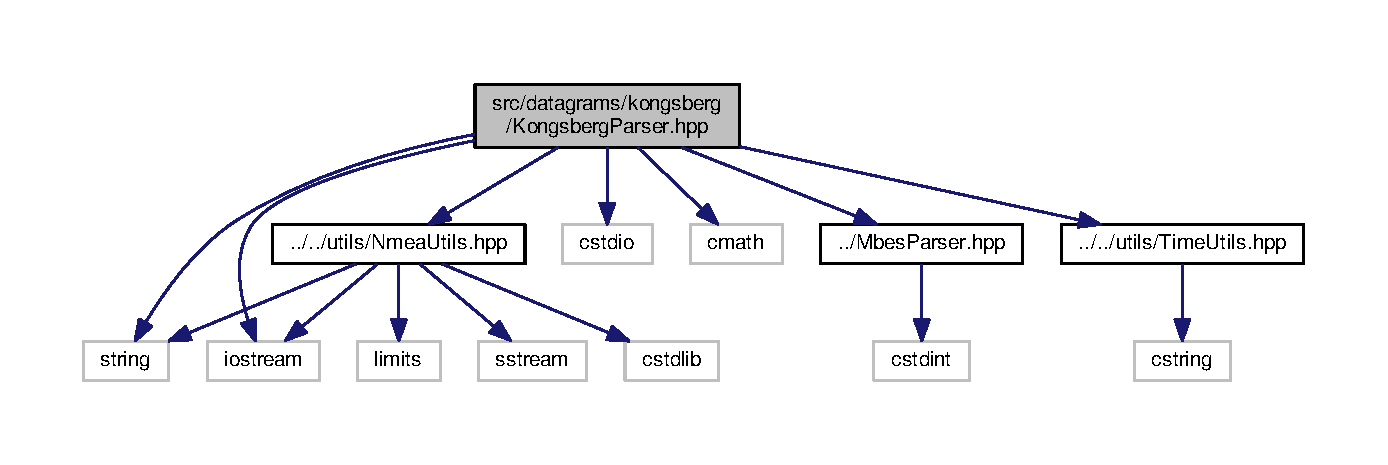
\includegraphics[width=350pt]{KongsbergParser_8hpp__incl}
\end{center}
\end{figure}
Ce graphe montre quels fichiers incluent directement ou indirectement ce fichier \+:
\nopagebreak
\begin{figure}[H]
\begin{center}
\leavevmode
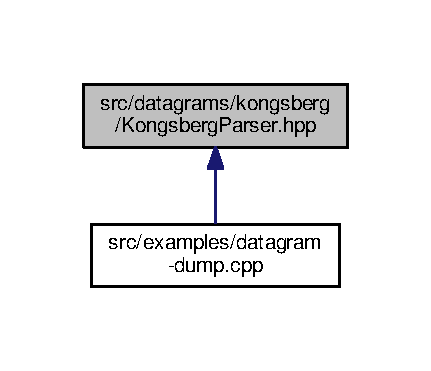
\includegraphics[width=207pt]{KongsbergParser_8hpp__dep__incl}
\end{center}
\end{figure}
\subsection*{Classes}
\begin{DoxyCompactItemize}
\item 
struct \hyperlink{structKongsbergHeader}{Kongsberg\+Header}
\item 
struct \hyperlink{structKongsbergAttitudeEntry}{Kongsberg\+Attitude\+Entry}
\item 
struct \hyperlink{structKongsbergPositionDatagram}{Kongsberg\+Position\+Datagram}
\item 
class \hyperlink{classKongsbergParser}{Kongsberg\+Parser}
\end{DoxyCompactItemize}
\subsection*{Macros}
\begin{DoxyCompactItemize}
\item 
\#define \hyperlink{KongsbergParser_8hpp_aacd744a917e61146ec8b7175b4761683}{S\+TX}~0x02
\item 
\#define \hyperlink{KongsbergParser_8hpp_af02558e983dd26832a852bf186ed6726}{E\+TX}~0x03https\+:
\end{DoxyCompactItemize}


\subsection{Documentation des macros}
\mbox{\Hypertarget{KongsbergParser_8hpp_af02558e983dd26832a852bf186ed6726}\label{KongsbergParser_8hpp_af02558e983dd26832a852bf186ed6726}} 
\index{Kongsberg\+Parser.\+hpp@{Kongsberg\+Parser.\+hpp}!E\+TX@{E\+TX}}
\index{E\+TX@{E\+TX}!Kongsberg\+Parser.\+hpp@{Kongsberg\+Parser.\+hpp}}
\subsubsection{\texorpdfstring{E\+TX}{ETX}}
{\footnotesize\ttfamily \#define E\+TX~0x03https\+:}

\mbox{\Hypertarget{KongsbergParser_8hpp_aacd744a917e61146ec8b7175b4761683}\label{KongsbergParser_8hpp_aacd744a917e61146ec8b7175b4761683}} 
\index{Kongsberg\+Parser.\+hpp@{Kongsberg\+Parser.\+hpp}!S\+TX@{S\+TX}}
\index{S\+TX@{S\+TX}!Kongsberg\+Parser.\+hpp@{Kongsberg\+Parser.\+hpp}}
\subsubsection{\texorpdfstring{S\+TX}{STX}}
{\footnotesize\ttfamily \#define S\+TX~0x02}


\hypertarget{KongsbergTypes_8hpp}{}\section{Référence du fichier src/datagrams/kongsberg/\+Kongsberg\+Types.hpp}
\label{KongsbergTypes_8hpp}\index{src/datagrams/kongsberg/\+Kongsberg\+Types.\+hpp@{src/datagrams/kongsberg/\+Kongsberg\+Types.\+hpp}}

\hypertarget{MbesParser_8hpp}{}\section{Référence du fichier src/datagrams/\+Mbes\+Parser.hpp}
\label{MbesParser_8hpp}\index{src/datagrams/\+Mbes\+Parser.\+hpp@{src/datagrams/\+Mbes\+Parser.\+hpp}}
{\ttfamily \#include $<$cstdint$>$}\newline
Graphe des dépendances par inclusion de Mbes\+Parser.\+hpp\+:
\nopagebreak
\begin{figure}[H]
\begin{center}
\leavevmode
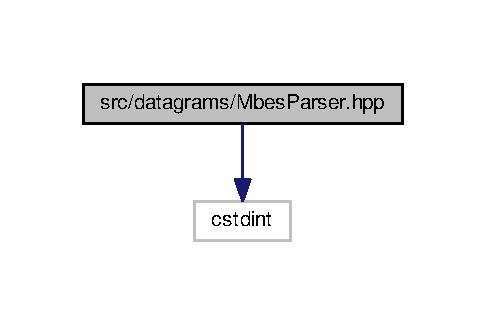
\includegraphics[width=233pt]{MbesParser_8hpp__incl}
\end{center}
\end{figure}
Ce graphe montre quels fichiers incluent directement ou indirectement ce fichier \+:
\nopagebreak
\begin{figure}[H]
\begin{center}
\leavevmode
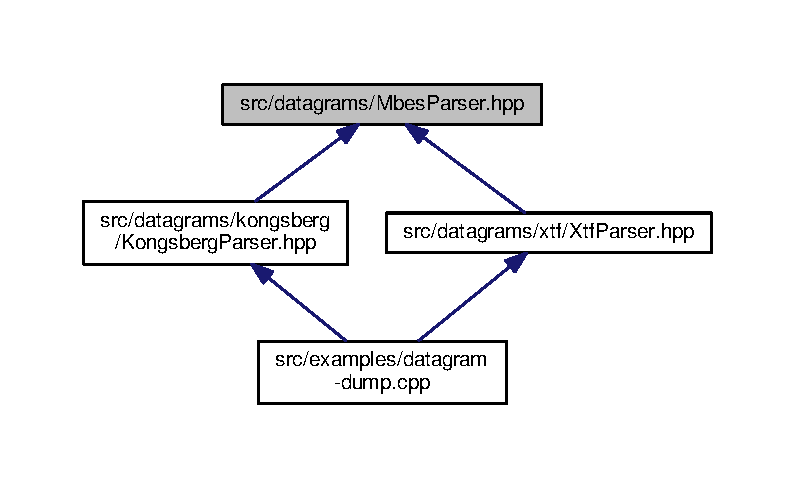
\includegraphics[width=350pt]{MbesParser_8hpp__dep__incl}
\end{center}
\end{figure}
\subsection*{Classes}
\begin{DoxyCompactItemize}
\item 
class \hyperlink{classMbesParser}{Mbes\+Parser}
\end{DoxyCompactItemize}

\hypertarget{XtfParser_8hpp}{}\section{Référence du fichier src/datagrams/xtf/\+Xtf\+Parser.hpp}
\label{XtfParser_8hpp}\index{src/datagrams/xtf/\+Xtf\+Parser.\+hpp@{src/datagrams/xtf/\+Xtf\+Parser.\+hpp}}
{\ttfamily \#include $<$string$>$}\newline
{\ttfamily \#include $<$stdio.\+h$>$}\newline
{\ttfamily \#include $<$string.\+h$>$}\newline
{\ttfamily \#include $<$cstdio$>$}\newline
{\ttfamily \#include \char`\"{}Xtf\+Types.\+hpp\char`\"{}}\newline
{\ttfamily \#include \char`\"{}../\+Mbes\+Parser.\+hpp\char`\"{}}\newline
{\ttfamily \#include \char`\"{}../../utils/\+Time\+Utils.\+hpp\char`\"{}}\newline
Graphe des dépendances par inclusion de Xtf\+Parser.\+hpp\+:
\nopagebreak
\begin{figure}[H]
\begin{center}
\leavevmode
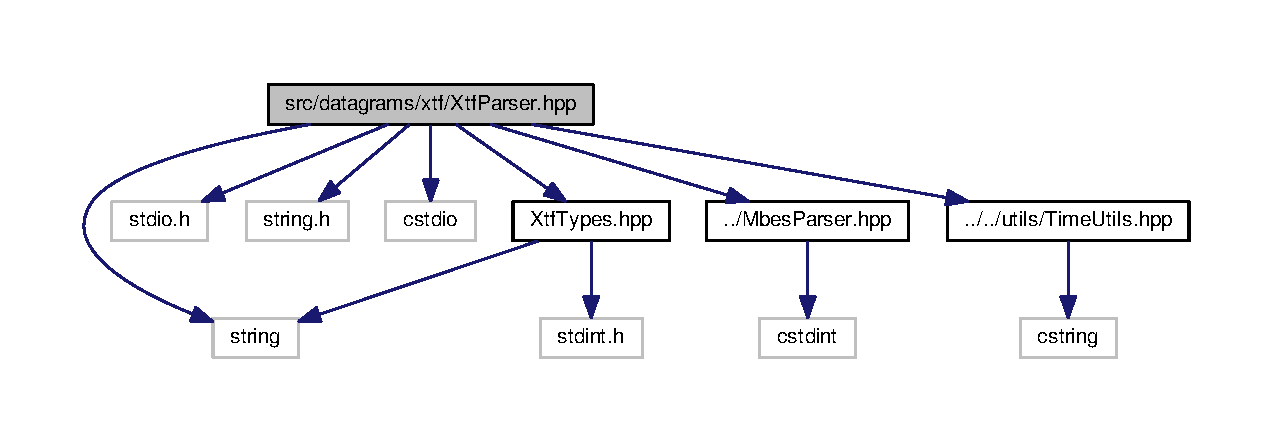
\includegraphics[width=350pt]{XtfParser_8hpp__incl}
\end{center}
\end{figure}
Ce graphe montre quels fichiers incluent directement ou indirectement ce fichier \+:
\nopagebreak
\begin{figure}[H]
\begin{center}
\leavevmode
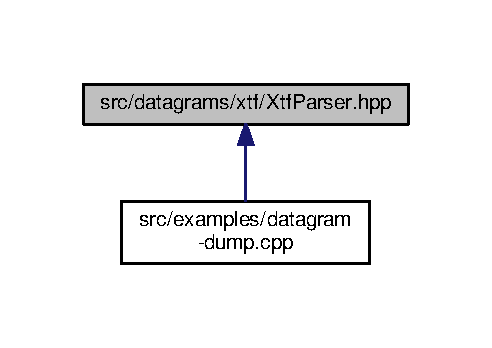
\includegraphics[width=236pt]{XtfParser_8hpp__dep__incl}
\end{center}
\end{figure}
\subsection*{Classes}
\begin{DoxyCompactItemize}
\item 
class \hyperlink{classXtfParser}{Xtf\+Parser}
\end{DoxyCompactItemize}
\subsection*{Macros}
\begin{DoxyCompactItemize}
\item 
\#define \hyperlink{XtfParser_8hpp_a54061e5993a5517320d425f44408cc86}{M\+A\+G\+I\+C\+\_\+\+N\+U\+M\+B\+ER}~123
\item 
\#define \hyperlink{XtfParser_8hpp_a9693ff683f2626abb6f01050d2a83704}{P\+A\+C\+K\+E\+T\+\_\+\+M\+A\+G\+I\+C\+\_\+\+N\+U\+M\+B\+ER}~0x\+F\+A\+CE
\end{DoxyCompactItemize}


\subsection{Documentation des macros}
\mbox{\Hypertarget{XtfParser_8hpp_a54061e5993a5517320d425f44408cc86}\label{XtfParser_8hpp_a54061e5993a5517320d425f44408cc86}} 
\index{Xtf\+Parser.\+hpp@{Xtf\+Parser.\+hpp}!M\+A\+G\+I\+C\+\_\+\+N\+U\+M\+B\+ER@{M\+A\+G\+I\+C\+\_\+\+N\+U\+M\+B\+ER}}
\index{M\+A\+G\+I\+C\+\_\+\+N\+U\+M\+B\+ER@{M\+A\+G\+I\+C\+\_\+\+N\+U\+M\+B\+ER}!Xtf\+Parser.\+hpp@{Xtf\+Parser.\+hpp}}
\subsubsection{\texorpdfstring{M\+A\+G\+I\+C\+\_\+\+N\+U\+M\+B\+ER}{MAGIC\_NUMBER}}
{\footnotesize\ttfamily \#define M\+A\+G\+I\+C\+\_\+\+N\+U\+M\+B\+ER~123}

\mbox{\Hypertarget{XtfParser_8hpp_a9693ff683f2626abb6f01050d2a83704}\label{XtfParser_8hpp_a9693ff683f2626abb6f01050d2a83704}} 
\index{Xtf\+Parser.\+hpp@{Xtf\+Parser.\+hpp}!P\+A\+C\+K\+E\+T\+\_\+\+M\+A\+G\+I\+C\+\_\+\+N\+U\+M\+B\+ER@{P\+A\+C\+K\+E\+T\+\_\+\+M\+A\+G\+I\+C\+\_\+\+N\+U\+M\+B\+ER}}
\index{P\+A\+C\+K\+E\+T\+\_\+\+M\+A\+G\+I\+C\+\_\+\+N\+U\+M\+B\+ER@{P\+A\+C\+K\+E\+T\+\_\+\+M\+A\+G\+I\+C\+\_\+\+N\+U\+M\+B\+ER}!Xtf\+Parser.\+hpp@{Xtf\+Parser.\+hpp}}
\subsubsection{\texorpdfstring{P\+A\+C\+K\+E\+T\+\_\+\+M\+A\+G\+I\+C\+\_\+\+N\+U\+M\+B\+ER}{PACKET\_MAGIC\_NUMBER}}
{\footnotesize\ttfamily \#define P\+A\+C\+K\+E\+T\+\_\+\+M\+A\+G\+I\+C\+\_\+\+N\+U\+M\+B\+ER~0x\+F\+A\+CE}


\hypertarget{XtfTypes_8hpp}{}\section{Référence du fichier src/datagrams/xtf/\+Xtf\+Types.hpp}
\label{XtfTypes_8hpp}\index{src/datagrams/xtf/\+Xtf\+Types.\+hpp@{src/datagrams/xtf/\+Xtf\+Types.\+hpp}}
{\ttfamily \#include $<$stdint.\+h$>$}\newline
{\ttfamily \#include $<$string$>$}\newline
Graphe des dépendances par inclusion de Xtf\+Types.\+hpp\+:
\nopagebreak
\begin{figure}[H]
\begin{center}
\leavevmode
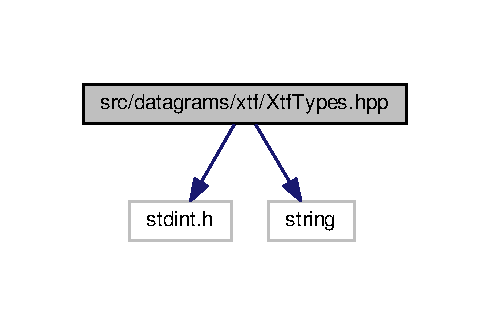
\includegraphics[width=235pt]{XtfTypes_8hpp__incl}
\end{center}
\end{figure}
Ce graphe montre quels fichiers incluent directement ou indirectement ce fichier \+:
\nopagebreak
\begin{figure}[H]
\begin{center}
\leavevmode
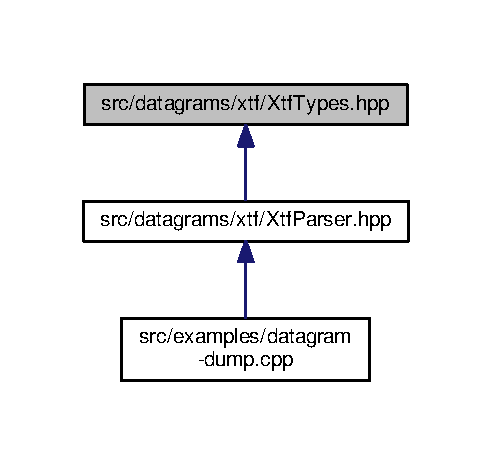
\includegraphics[width=236pt]{XtfTypes_8hpp__dep__incl}
\end{center}
\end{figure}
\subsection*{Classes}
\begin{DoxyCompactItemize}
\item 
struct \hyperlink{structXtfChanInfo}{Xtf\+Chan\+Info}
\begin{DoxyCompactList}\small\item\em Description des datagrammes pour le format X\+TF Référence\+: Triton Imaging, Inc. \end{DoxyCompactList}\item 
struct \hyperlink{structXtfFileHeader}{Xtf\+File\+Header}
\item 
struct \hyperlink{structXtfPacketHeader}{Xtf\+Packet\+Header}
\item 
struct \hyperlink{structXtfPingHeader}{Xtf\+Ping\+Header}
\item 
struct \hyperlink{structXtfPingChanHeader}{Xtf\+Ping\+Chan\+Header}
\item 
struct \hyperlink{structXtfNotesHeader}{Xtf\+Notes\+Header}
\item 
struct \hyperlink{structXtfAttitudeData}{Xtf\+Attitude\+Data}
\item 
struct \hyperlink{structXtfRawSerialHeader}{Xtf\+Raw\+Serial\+Header}
\item 
struct \hyperlink{structXtfHighSpeedSensor}{Xtf\+High\+Speed\+Sensor}
\item 
struct \hyperlink{structXtfBeamXYZA}{Xtf\+Beam\+X\+Y\+ZA}
\item 
struct \hyperlink{structSNP0}{S\+N\+P0}
\item 
struct \hyperlink{structSNP1}{S\+N\+P1}
\item 
struct \hyperlink{structXtfPosRawNavigation}{Xtf\+Pos\+Raw\+Navigation}
\item 
struct \hyperlink{structXtfQpsSingleBeam}{Xtf\+Qps\+Single\+Beam}
\item 
struct \hyperlink{structXtfQpsMultiTxEntry}{Xtf\+Qps\+Multi\+Tx\+Entry}
\item 
struct \hyperlink{structXtfQpsMbEntry}{Xtf\+Qps\+Mb\+Entry}
\item 
struct \hyperlink{structXtfRawCustomHeader}{Xtf\+Raw\+Custom\+Header}
\item 
struct \hyperlink{structXtfHeaderNavigation__type42}{Xtf\+Header\+Navigation\+\_\+type42}
\item 
struct \hyperlink{structXtfHeaderNavigation__type84}{Xtf\+Header\+Navigation\+\_\+type84}
\item 
struct \hyperlink{structXtfHeaderGyro}{Xtf\+Header\+Gyro}
\end{DoxyCompactItemize}
\subsection*{Macros}
\begin{DoxyCompactItemize}
\item 
\#define \hyperlink{XtfTypes_8hpp_ac90689fcd3e08e86710f1c6002620a2d}{X\+T\+F\+\_\+\+H\+E\+A\+D\+E\+R\+\_\+\+A\+T\+T\+I\+T\+U\+DE}~3
\item 
\#define \hyperlink{XtfTypes_8hpp_ab238b1c2675a55903e206d64ca19248e}{X\+T\+F\+\_\+\+H\+E\+A\+D\+E\+R\+\_\+\+Q\+\_\+\+M\+U\+L\+T\+I\+B\+E\+AM}~28
\item 
\#define \hyperlink{XtfTypes_8hpp_a1025438728e34895363a2340fe84a10e}{X\+T\+F\+\_\+\+H\+E\+A\+D\+E\+R\+\_\+\+P\+O\+S\+I\+T\+I\+ON}~107
\end{DoxyCompactItemize}
\subsection*{Variables}
\begin{DoxyCompactItemize}
\item 
const std\+::string \hyperlink{XtfTypes_8hpp_a5e9899f20b840e345e65ee8115f029d7}{Sonar\+Types} \mbox{[}$\,$\mbox{]}
\end{DoxyCompactItemize}


\subsection{Documentation des macros}
\mbox{\Hypertarget{XtfTypes_8hpp_ac90689fcd3e08e86710f1c6002620a2d}\label{XtfTypes_8hpp_ac90689fcd3e08e86710f1c6002620a2d}} 
\index{Xtf\+Types.\+hpp@{Xtf\+Types.\+hpp}!X\+T\+F\+\_\+\+H\+E\+A\+D\+E\+R\+\_\+\+A\+T\+T\+I\+T\+U\+DE@{X\+T\+F\+\_\+\+H\+E\+A\+D\+E\+R\+\_\+\+A\+T\+T\+I\+T\+U\+DE}}
\index{X\+T\+F\+\_\+\+H\+E\+A\+D\+E\+R\+\_\+\+A\+T\+T\+I\+T\+U\+DE@{X\+T\+F\+\_\+\+H\+E\+A\+D\+E\+R\+\_\+\+A\+T\+T\+I\+T\+U\+DE}!Xtf\+Types.\+hpp@{Xtf\+Types.\+hpp}}
\subsubsection{\texorpdfstring{X\+T\+F\+\_\+\+H\+E\+A\+D\+E\+R\+\_\+\+A\+T\+T\+I\+T\+U\+DE}{XTF\_HEADER\_ATTITUDE}}
{\footnotesize\ttfamily \#define X\+T\+F\+\_\+\+H\+E\+A\+D\+E\+R\+\_\+\+A\+T\+T\+I\+T\+U\+DE~3}

\mbox{\Hypertarget{XtfTypes_8hpp_a1025438728e34895363a2340fe84a10e}\label{XtfTypes_8hpp_a1025438728e34895363a2340fe84a10e}} 
\index{Xtf\+Types.\+hpp@{Xtf\+Types.\+hpp}!X\+T\+F\+\_\+\+H\+E\+A\+D\+E\+R\+\_\+\+P\+O\+S\+I\+T\+I\+ON@{X\+T\+F\+\_\+\+H\+E\+A\+D\+E\+R\+\_\+\+P\+O\+S\+I\+T\+I\+ON}}
\index{X\+T\+F\+\_\+\+H\+E\+A\+D\+E\+R\+\_\+\+P\+O\+S\+I\+T\+I\+ON@{X\+T\+F\+\_\+\+H\+E\+A\+D\+E\+R\+\_\+\+P\+O\+S\+I\+T\+I\+ON}!Xtf\+Types.\+hpp@{Xtf\+Types.\+hpp}}
\subsubsection{\texorpdfstring{X\+T\+F\+\_\+\+H\+E\+A\+D\+E\+R\+\_\+\+P\+O\+S\+I\+T\+I\+ON}{XTF\_HEADER\_POSITION}}
{\footnotesize\ttfamily \#define X\+T\+F\+\_\+\+H\+E\+A\+D\+E\+R\+\_\+\+P\+O\+S\+I\+T\+I\+ON~107}

\mbox{\Hypertarget{XtfTypes_8hpp_ab238b1c2675a55903e206d64ca19248e}\label{XtfTypes_8hpp_ab238b1c2675a55903e206d64ca19248e}} 
\index{Xtf\+Types.\+hpp@{Xtf\+Types.\+hpp}!X\+T\+F\+\_\+\+H\+E\+A\+D\+E\+R\+\_\+\+Q\+\_\+\+M\+U\+L\+T\+I\+B\+E\+AM@{X\+T\+F\+\_\+\+H\+E\+A\+D\+E\+R\+\_\+\+Q\+\_\+\+M\+U\+L\+T\+I\+B\+E\+AM}}
\index{X\+T\+F\+\_\+\+H\+E\+A\+D\+E\+R\+\_\+\+Q\+\_\+\+M\+U\+L\+T\+I\+B\+E\+AM@{X\+T\+F\+\_\+\+H\+E\+A\+D\+E\+R\+\_\+\+Q\+\_\+\+M\+U\+L\+T\+I\+B\+E\+AM}!Xtf\+Types.\+hpp@{Xtf\+Types.\+hpp}}
\subsubsection{\texorpdfstring{X\+T\+F\+\_\+\+H\+E\+A\+D\+E\+R\+\_\+\+Q\+\_\+\+M\+U\+L\+T\+I\+B\+E\+AM}{XTF\_HEADER\_Q\_MULTIBEAM}}
{\footnotesize\ttfamily \#define X\+T\+F\+\_\+\+H\+E\+A\+D\+E\+R\+\_\+\+Q\+\_\+\+M\+U\+L\+T\+I\+B\+E\+AM~28}



\subsection{Documentation des variables}
\mbox{\Hypertarget{XtfTypes_8hpp_a5e9899f20b840e345e65ee8115f029d7}\label{XtfTypes_8hpp_a5e9899f20b840e345e65ee8115f029d7}} 
\index{Xtf\+Types.\+hpp@{Xtf\+Types.\+hpp}!Sonar\+Types@{Sonar\+Types}}
\index{Sonar\+Types@{Sonar\+Types}!Xtf\+Types.\+hpp@{Xtf\+Types.\+hpp}}
\subsubsection{\texorpdfstring{Sonar\+Types}{SonarTypes}}
{\footnotesize\ttfamily const std\+::string Sonar\+Types\mbox{[}$\,$\mbox{]}}


\hypertarget{datagram-dump_8cpp}{}\section{Référence du fichier src/examples/datagram-\/dump.cpp}
\label{datagram-dump_8cpp}\index{src/examples/datagram-\/dump.\+cpp@{src/examples/datagram-\/dump.\+cpp}}
{\ttfamily \#include $<$getopt.\+h$>$}\newline
{\ttfamily \#include \char`\"{}../datagrams/kongsberg/\+Kongsberg\+Parser.\+hpp\char`\"{}}\newline
{\ttfamily \#include \char`\"{}../datagrams/xtf/\+Xtf\+Parser.\+hpp\char`\"{}}\newline
{\ttfamily \#include $<$iostream$>$}\newline
{\ttfamily \#include $<$string$>$}\newline
{\ttfamily \#include \char`\"{}../utils/\+String\+Utils.\+hpp\char`\"{}}\newline
Graphe des dépendances par inclusion de datagram-\/dump.cpp\+:
\nopagebreak
\begin{figure}[H]
\begin{center}
\leavevmode
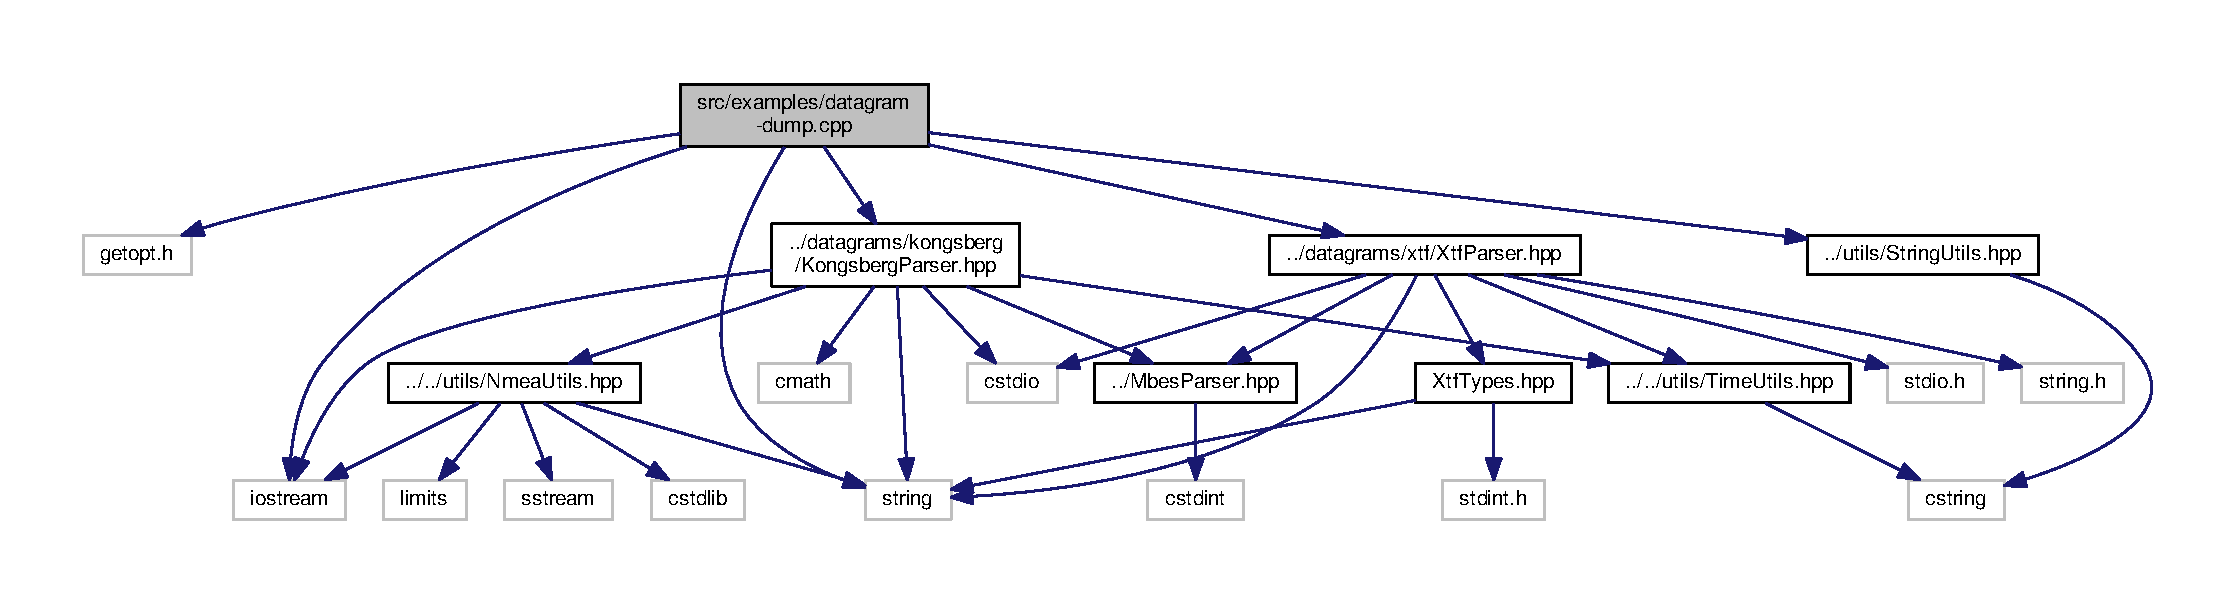
\includegraphics[width=350pt]{datagram-dump_8cpp__incl}
\end{center}
\end{figure}
\subsection*{Macros}
\begin{DoxyCompactItemize}
\item 
\#define \hyperlink{datagram-dump_8cpp_af6b0b7a8cf49a8aafda02b6d9c6085d6}{M\+A\+I\+N\+\_\+\+C\+PP}
\end{DoxyCompactItemize}
\subsection*{Fonctions}
\begin{DoxyCompactItemize}
\item 
void \hyperlink{datagram-dump_8cpp_aead97c99e70c0da7036fbbe230ef68b6}{print\+Usage} ()
\item 
int \hyperlink{datagram-dump_8cpp_a3c04138a5bfe5d72780bb7e82a18e627}{main} (int argc, char $\ast$$\ast$argv)
\end{DoxyCompactItemize}


\subsection{Documentation des macros}
\mbox{\Hypertarget{datagram-dump_8cpp_af6b0b7a8cf49a8aafda02b6d9c6085d6}\label{datagram-dump_8cpp_af6b0b7a8cf49a8aafda02b6d9c6085d6}} 
\index{datagram-\/dump.\+cpp@{datagram-\/dump.\+cpp}!M\+A\+I\+N\+\_\+\+C\+PP@{M\+A\+I\+N\+\_\+\+C\+PP}}
\index{M\+A\+I\+N\+\_\+\+C\+PP@{M\+A\+I\+N\+\_\+\+C\+PP}!datagram-\/dump.\+cpp@{datagram-\/dump.\+cpp}}
\subsubsection{\texorpdfstring{M\+A\+I\+N\+\_\+\+C\+PP}{MAIN\_CPP}}
{\footnotesize\ttfamily \#define M\+A\+I\+N\+\_\+\+C\+PP}



\subsection{Documentation des fonctions}
\mbox{\Hypertarget{datagram-dump_8cpp_a3c04138a5bfe5d72780bb7e82a18e627}\label{datagram-dump_8cpp_a3c04138a5bfe5d72780bb7e82a18e627}} 
\index{datagram-\/dump.\+cpp@{datagram-\/dump.\+cpp}!main@{main}}
\index{main@{main}!datagram-\/dump.\+cpp@{datagram-\/dump.\+cpp}}
\subsubsection{\texorpdfstring{main()}{main()}}
{\footnotesize\ttfamily int main (\begin{DoxyParamCaption}\item[{int}]{argc,  }\item[{char $\ast$$\ast$}]{argv }\end{DoxyParamCaption})}

\mbox{\Hypertarget{datagram-dump_8cpp_aead97c99e70c0da7036fbbe230ef68b6}\label{datagram-dump_8cpp_aead97c99e70c0da7036fbbe230ef68b6}} 
\index{datagram-\/dump.\+cpp@{datagram-\/dump.\+cpp}!print\+Usage@{print\+Usage}}
\index{print\+Usage@{print\+Usage}!datagram-\/dump.\+cpp@{datagram-\/dump.\+cpp}}
\subsubsection{\texorpdfstring{print\+Usage()}{printUsage()}}
{\footnotesize\ttfamily void print\+Usage (\begin{DoxyParamCaption}{ }\end{DoxyParamCaption})}


\hypertarget{NmeaUtils_8hpp}{}\section{Référence du fichier src/utils/\+Nmea\+Utils.hpp}
\label{NmeaUtils_8hpp}\index{src/utils/\+Nmea\+Utils.\+hpp@{src/utils/\+Nmea\+Utils.\+hpp}}
{\ttfamily \#include $<$limits$>$}\newline
{\ttfamily \#include $<$string$>$}\newline
{\ttfamily \#include $<$sstream$>$}\newline
{\ttfamily \#include $<$iostream$>$}\newline
{\ttfamily \#include $<$cstdlib$>$}\newline
Graphe des dépendances par inclusion de Nmea\+Utils.\+hpp\+:
\nopagebreak
\begin{figure}[H]
\begin{center}
\leavevmode
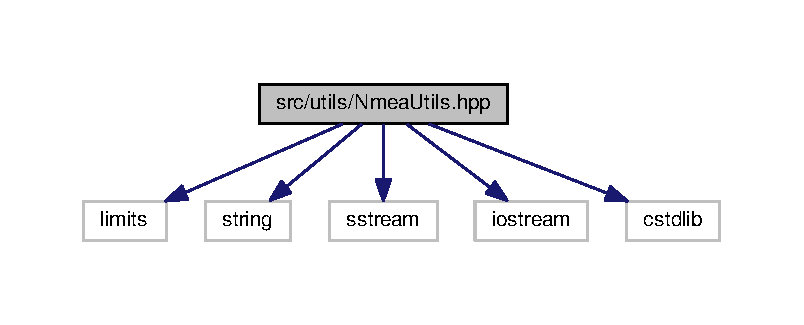
\includegraphics[width=350pt]{NmeaUtils_8hpp__incl}
\end{center}
\end{figure}
Ce graphe montre quels fichiers incluent directement ou indirectement ce fichier \+:
\nopagebreak
\begin{figure}[H]
\begin{center}
\leavevmode
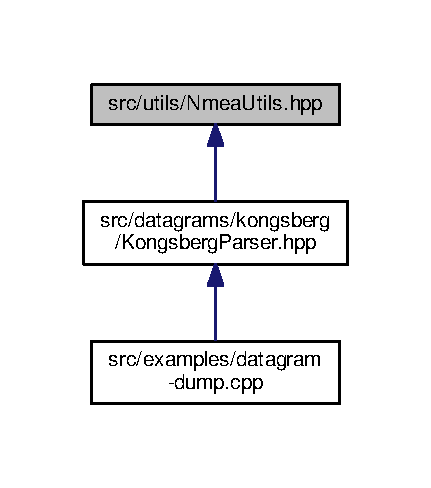
\includegraphics[width=207pt]{NmeaUtils_8hpp__dep__incl}
\end{center}
\end{figure}
\subsection*{Classes}
\begin{DoxyCompactItemize}
\item 
class \hyperlink{classNmeaUtils}{Nmea\+Utils}
\end{DoxyCompactItemize}

\hypertarget{StringUtils_8hpp}{}\section{Référence du fichier src/utils/\+String\+Utils.hpp}
\label{StringUtils_8hpp}\index{src/utils/\+String\+Utils.\+hpp@{src/utils/\+String\+Utils.\+hpp}}
{\ttfamily \#include $<$cstring$>$}\newline
Graphe des dépendances par inclusion de String\+Utils.\+hpp\+:
\nopagebreak
\begin{figure}[H]
\begin{center}
\leavevmode
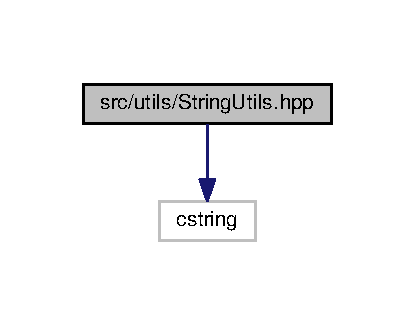
\includegraphics[width=199pt]{StringUtils_8hpp__incl}
\end{center}
\end{figure}
Ce graphe montre quels fichiers incluent directement ou indirectement ce fichier \+:
\nopagebreak
\begin{figure}[H]
\begin{center}
\leavevmode
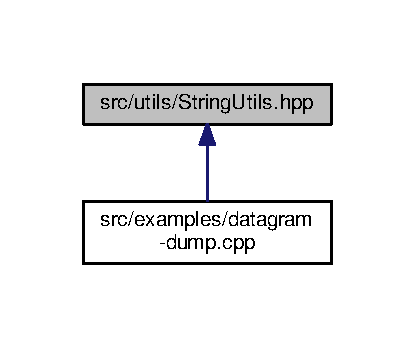
\includegraphics[width=199pt]{StringUtils_8hpp__dep__incl}
\end{center}
\end{figure}
\subsection*{Fonctions}
\begin{DoxyCompactItemize}
\item 
int \hyperlink{StringUtils_8hpp_a138015330cc0ee5dcb0c6504c3166754}{ends\+\_\+with} (const char $\ast$str, const char $\ast$suffix)
\end{DoxyCompactItemize}


\subsection{Documentation des fonctions}
\mbox{\Hypertarget{StringUtils_8hpp_a138015330cc0ee5dcb0c6504c3166754}\label{StringUtils_8hpp_a138015330cc0ee5dcb0c6504c3166754}} 
\index{String\+Utils.\+hpp@{String\+Utils.\+hpp}!ends\+\_\+with@{ends\+\_\+with}}
\index{ends\+\_\+with@{ends\+\_\+with}!String\+Utils.\+hpp@{String\+Utils.\+hpp}}
\subsubsection{\texorpdfstring{ends\+\_\+with()}{ends\_with()}}
{\footnotesize\ttfamily int ends\+\_\+with (\begin{DoxyParamCaption}\item[{const char $\ast$}]{str,  }\item[{const char $\ast$}]{suffix }\end{DoxyParamCaption})}


\hypertarget{TimeUtils_8hpp}{}\section{Référence du fichier src/utils/\+Time\+Utils.hpp}
\label{TimeUtils_8hpp}\index{src/utils/\+Time\+Utils.\+hpp@{src/utils/\+Time\+Utils.\+hpp}}
{\ttfamily \#include $<$cstring$>$}\newline
Graphe des dépendances par inclusion de Time\+Utils.\+hpp\+:
\nopagebreak
\begin{figure}[H]
\begin{center}
\leavevmode
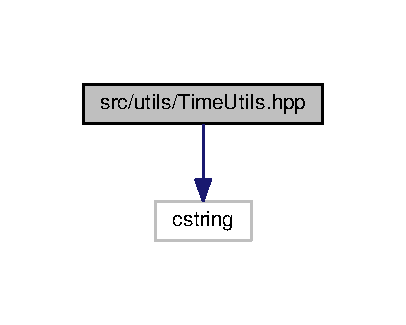
\includegraphics[width=195pt]{TimeUtils_8hpp__incl}
\end{center}
\end{figure}
Ce graphe montre quels fichiers incluent directement ou indirectement ce fichier \+:
\nopagebreak
\begin{figure}[H]
\begin{center}
\leavevmode
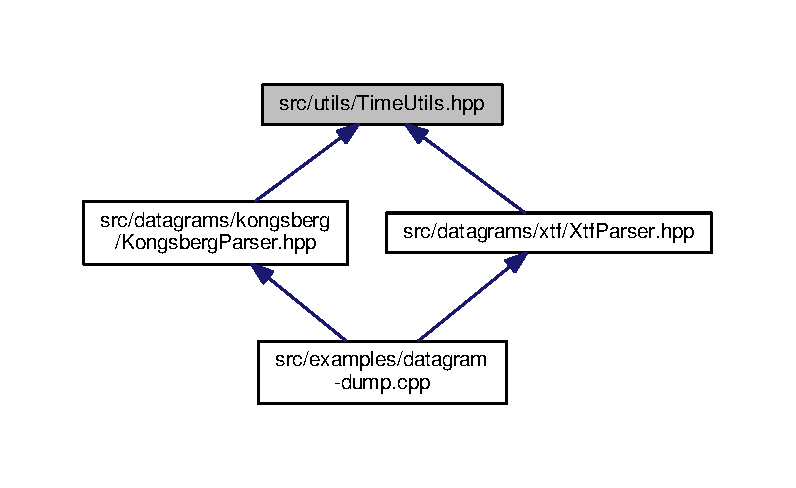
\includegraphics[width=350pt]{TimeUtils_8hpp__dep__incl}
\end{center}
\end{figure}
\subsection*{Fonctions}
\begin{DoxyCompactItemize}
\item 
uint64\+\_\+t \hyperlink{TimeUtils_8hpp_ae48dd25c99eca9438609cb0ecea0e31d}{build\+\_\+time} (int year, int month, int day, int hour, int minutes, int seconds, int millis, int microseconds)
\begin{DoxyCompactList}\small\item\em Returns epoch in microseconds since Jan 1 1970. \end{DoxyCompactList}\item 
uint64\+\_\+t \hyperlink{TimeUtils_8hpp_ad67f5318180ce6451c07bc757881b67a}{build\+\_\+time} (int year, int month, int day, long time\+In\+Milliseconds)
\begin{DoxyCompactList}\small\item\em Returns epoch in microseconds since Jan 1 1970. \end{DoxyCompactList}\end{DoxyCompactItemize}


\subsection{Documentation des fonctions}
\mbox{\Hypertarget{TimeUtils_8hpp_ae48dd25c99eca9438609cb0ecea0e31d}\label{TimeUtils_8hpp_ae48dd25c99eca9438609cb0ecea0e31d}} 
\index{Time\+Utils.\+hpp@{Time\+Utils.\+hpp}!build\+\_\+time@{build\+\_\+time}}
\index{build\+\_\+time@{build\+\_\+time}!Time\+Utils.\+hpp@{Time\+Utils.\+hpp}}
\subsubsection{\texorpdfstring{build\+\_\+time()}{build\_time()}\hspace{0.1cm}{\footnotesize\ttfamily [1/2]}}
{\footnotesize\ttfamily uint64\+\_\+t build\+\_\+time (\begin{DoxyParamCaption}\item[{int}]{year,  }\item[{int}]{month,  }\item[{int}]{day,  }\item[{int}]{hour,  }\item[{int}]{minutes,  }\item[{int}]{seconds,  }\item[{int}]{millis,  }\item[{int}]{microseconds }\end{DoxyParamCaption})}



Returns epoch in microseconds since Jan 1 1970. 

\mbox{\Hypertarget{TimeUtils_8hpp_ad67f5318180ce6451c07bc757881b67a}\label{TimeUtils_8hpp_ad67f5318180ce6451c07bc757881b67a}} 
\index{Time\+Utils.\+hpp@{Time\+Utils.\+hpp}!build\+\_\+time@{build\+\_\+time}}
\index{build\+\_\+time@{build\+\_\+time}!Time\+Utils.\+hpp@{Time\+Utils.\+hpp}}
\subsubsection{\texorpdfstring{build\+\_\+time()}{build\_time()}\hspace{0.1cm}{\footnotesize\ttfamily [2/2]}}
{\footnotesize\ttfamily uint64\+\_\+t build\+\_\+time (\begin{DoxyParamCaption}\item[{int}]{year,  }\item[{int}]{month,  }\item[{int}]{day,  }\item[{long}]{time\+In\+Milliseconds }\end{DoxyParamCaption})}



Returns epoch in microseconds since Jan 1 1970. 

Time includes hours and minutes since midnight 
%--- End generated contents ---

% Index
\backmatter
\newpage
\phantomsection
\clearemptydoublepage
\addcontentsline{toc}{chapter}{Index}
\printindex

\end{document}
